\documentclass[a4paper]{book}
\usepackage{a4wide}
\usepackage{makeidx}
\usepackage{graphicx}
\usepackage{multicol}
\usepackage{float}
\usepackage{listings}
\usepackage{color}
\usepackage{textcomp}
\usepackage{alltt}
\usepackage{times}
\usepackage{ifpdf}
\ifpdf
\usepackage[pdftex,
            pagebackref=true,
            colorlinks=true,
            linkcolor=blue,
            unicode
           ]{hyperref}
\else
\usepackage[ps2pdf,
            pagebackref=true,
            colorlinks=true,
            linkcolor=blue,
            unicode
           ]{hyperref}
\usepackage{pspicture}
\fi
\usepackage[utf8]{inputenc}
\usepackage{doxygen}
\lstset{language=C++,inputencoding=utf8,basicstyle=\footnotesize,breaklines=true,breakatwhitespace=true,tabsize=8,numbers=left }
\makeindex
\setcounter{tocdepth}{3}
\renewcommand{\footrulewidth}{0.4pt}
\begin{document}
\hypersetup{pageanchor=false}
\begin{titlepage}
\vspace*{7cm}
\begin{center}
{\Large EvoDeMo }\\
\vspace*{1cm}
{\large Generated by Doxygen 1.6.1}\\
\vspace*{0.5cm}
{\small Fri May 14 00:51:03 2010}\\
\end{center}
\end{titlepage}
\clearemptydoublepage
\pagenumbering{roman}
\tableofcontents
\clearemptydoublepage
\pagenumbering{arabic}
\hypersetup{pageanchor=true}
\chapter{Class Index}
\section{Class Hierarchy}
This inheritance list is sorted roughly, but not completely, alphabetically:\begin{DoxyCompactList}
\item \contentsline{section}{CArray2d}{\pageref{classCArray2d}}{}
\begin{DoxyCompactList}
\item \contentsline{section}{CSpace}{\pageref{classCSpace}}{}
\end{DoxyCompactList}
\item \contentsline{section}{CCellularAutomata}{\pageref{classCCellularAutomata}}{}
\item \contentsline{section}{CConfigCore}{\pageref{classCConfigCore}}{}
\item \contentsline{section}{CCore}{\pageref{classCCore}}{}
\item \contentsline{section}{CCrossover}{\pageref{classCCrossover}}{}
\item \contentsline{section}{CExportCA}{\pageref{classCExportCA}}{}
\item \contentsline{section}{CExportConfig}{\pageref{classCExportConfig}}{}
\item \contentsline{section}{CExportGA}{\pageref{classCExportGA}}{}
\item \contentsline{section}{CExportLog}{\pageref{classCExportLog}}{}
\item \contentsline{section}{CFitness}{\pageref{classCFitness}}{}
\item \contentsline{section}{CGeneticAlgorithm}{\pageref{classCGeneticAlgorithm}}{}
\item \contentsline{section}{CGenome}{\pageref{classCGenome}}{}
\item \contentsline{section}{CGenomeType2}{\pageref{classCGenomeType2}}{}
\item \contentsline{section}{CGenomeType2\_\-Ins}{\pageref{classCGenomeType2__Ins}}{}
\item \contentsline{section}{CGenomeType2\_\-Nbh5}{\pageref{classCGenomeType2__Nbh5}}{}
\item \contentsline{section}{CGenomeType3}{\pageref{classCGenomeType3}}{}
\item \contentsline{section}{CGenomeType3\_\-Nbh5}{\pageref{classCGenomeType3__Nbh5}}{}
\item \contentsline{section}{CGenomeType4}{\pageref{classCGenomeType4}}{}
\item \contentsline{section}{CGenomeType4\_\-Nbh5}{\pageref{classCGenomeType4__Nbh5}}{}
\item \contentsline{section}{CGraphicsItem}{\pageref{classCGraphicsItem}}{}
\item \contentsline{section}{CGraphicsItemConfig}{\pageref{classCGraphicsItemConfig}}{}
\item \contentsline{section}{CGraphicsScene}{\pageref{classCGraphicsScene}}{}
\item \contentsline{section}{CGraphicsView}{\pageref{classCGraphicsView}}{}
\item \contentsline{section}{CImportConfig}{\pageref{classCImportConfig}}{}
\item \contentsline{section}{CImportGA}{\pageref{classCImportGA}}{}
\item \contentsline{section}{CInputCA}{\pageref{classCInputCA}}{}
\item \contentsline{section}{CMutation}{\pageref{classCMutation}}{}
\item \contentsline{section}{CRandom}{\pageref{classCRandom}}{}
\item \contentsline{section}{CRulesTable}{\pageref{classCRulesTable}}{}
\item \contentsline{section}{CSelection}{\pageref{classCSelection}}{}
\item \contentsline{section}{CTFunction}{\pageref{classCTFunction}}{}
\item \contentsline{section}{CThreadCore}{\pageref{classCThreadCore}}{}
\item \contentsline{section}{CWidgetEvolution}{\pageref{classCWidgetEvolution}}{}
\item \contentsline{section}{CWidgetExport}{\pageref{classCWidgetExport}}{}
\item \contentsline{section}{CWidgetInput}{\pageref{classCWidgetInput}}{}
\item \contentsline{section}{CWidgetOutput}{\pageref{classCWidgetOutput}}{}
\item \contentsline{section}{CWidgetRunCA}{\pageref{classCWidgetRunCA}}{}
\item \contentsline{section}{CWidgetRunEvo}{\pageref{classCWidgetRunEvo}}{}
\item \contentsline{section}{CWindowMain}{\pageref{classCWindowMain}}{}
\item \contentsline{section}{stArray}{\pageref{structstArray}}{}
\item \contentsline{section}{stGeneInstruction}{\pageref{structstGeneInstruction}}{}
\item \contentsline{section}{stThreadCoreDataGA}{\pageref{structstThreadCoreDataGA}}{}
\end{DoxyCompactList}

\chapter{Class Index}
\section{Class List}
Here are the classes, structs, unions and interfaces with brief descriptions:\begin{DoxyCompactList}
\item\contentsline{section}{\hyperlink{classCArray2d}{CArray2d} }{\pageref{classCArray2d}}{}
\item\contentsline{section}{\hyperlink{classCCellularAutomata}{CCellularAutomata} }{\pageref{classCCellularAutomata}}{}
\item\contentsline{section}{\hyperlink{classCConfigCore}{CConfigCore} }{\pageref{classCConfigCore}}{}
\item\contentsline{section}{\hyperlink{classCCore}{CCore} }{\pageref{classCCore}}{}
\item\contentsline{section}{\hyperlink{classCCrossover}{CCrossover} }{\pageref{classCCrossover}}{}
\item\contentsline{section}{\hyperlink{classCExportCA}{CExportCA} }{\pageref{classCExportCA}}{}
\item\contentsline{section}{\hyperlink{classCExportConfig}{CExportConfig} }{\pageref{classCExportConfig}}{}
\item\contentsline{section}{\hyperlink{classCExportGA}{CExportGA} }{\pageref{classCExportGA}}{}
\item\contentsline{section}{\hyperlink{classCExportLog}{CExportLog} }{\pageref{classCExportLog}}{}
\item\contentsline{section}{\hyperlink{classCFitness}{CFitness} }{\pageref{classCFitness}}{}
\item\contentsline{section}{\hyperlink{classCGeneticAlgorithm}{CGeneticAlgorithm} }{\pageref{classCGeneticAlgorithm}}{}
\item\contentsline{section}{\hyperlink{classCGenome}{CGenome} }{\pageref{classCGenome}}{}
\item\contentsline{section}{\hyperlink{classCGenomeType2}{CGenomeType2} }{\pageref{classCGenomeType2}}{}
\item\contentsline{section}{\hyperlink{classCGenomeType2__Ins}{CGenomeType2\_\-Ins} }{\pageref{classCGenomeType2__Ins}}{}
\item\contentsline{section}{\hyperlink{classCGenomeType2__Nbh5}{CGenomeType2\_\-Nbh5} }{\pageref{classCGenomeType2__Nbh5}}{}
\item\contentsline{section}{\hyperlink{classCGenomeType3}{CGenomeType3} }{\pageref{classCGenomeType3}}{}
\item\contentsline{section}{\hyperlink{classCGenomeType3__Nbh5}{CGenomeType3\_\-Nbh5} }{\pageref{classCGenomeType3__Nbh5}}{}
\item\contentsline{section}{\hyperlink{classCGenomeType4}{CGenomeType4} }{\pageref{classCGenomeType4}}{}
\item\contentsline{section}{\hyperlink{classCGenomeType4__Nbh5}{CGenomeType4\_\-Nbh5} }{\pageref{classCGenomeType4__Nbh5}}{}
\item\contentsline{section}{\hyperlink{classCGraphicsItem}{CGraphicsItem} }{\pageref{classCGraphicsItem}}{}
\item\contentsline{section}{\hyperlink{classCGraphicsItemConfig}{CGraphicsItemConfig} }{\pageref{classCGraphicsItemConfig}}{}
\item\contentsline{section}{\hyperlink{classCGraphicsScene}{CGraphicsScene} }{\pageref{classCGraphicsScene}}{}
\item\contentsline{section}{\hyperlink{classCGraphicsView}{CGraphicsView} }{\pageref{classCGraphicsView}}{}
\item\contentsline{section}{\hyperlink{classCImportConfig}{CImportConfig} }{\pageref{classCImportConfig}}{}
\item\contentsline{section}{\hyperlink{classCImportGA}{CImportGA} }{\pageref{classCImportGA}}{}
\item\contentsline{section}{\hyperlink{classCInputCA}{CInputCA} }{\pageref{classCInputCA}}{}
\item\contentsline{section}{\hyperlink{classCMutation}{CMutation} }{\pageref{classCMutation}}{}
\item\contentsline{section}{\hyperlink{classCRandom}{CRandom} }{\pageref{classCRandom}}{}
\item\contentsline{section}{\hyperlink{classCRulesTable}{CRulesTable} }{\pageref{classCRulesTable}}{}
\item\contentsline{section}{\hyperlink{classCSelection}{CSelection} }{\pageref{classCSelection}}{}
\item\contentsline{section}{\hyperlink{classCSpace}{CSpace} }{\pageref{classCSpace}}{}
\item\contentsline{section}{\hyperlink{classCTFunction}{CTFunction} }{\pageref{classCTFunction}}{}
\item\contentsline{section}{\hyperlink{classCThreadCore}{CThreadCore} }{\pageref{classCThreadCore}}{}
\item\contentsline{section}{\hyperlink{classCWidgetEvolution}{CWidgetEvolution} }{\pageref{classCWidgetEvolution}}{}
\item\contentsline{section}{\hyperlink{classCWidgetExport}{CWidgetExport} }{\pageref{classCWidgetExport}}{}
\item\contentsline{section}{\hyperlink{classCWidgetInput}{CWidgetInput} }{\pageref{classCWidgetInput}}{}
\item\contentsline{section}{\hyperlink{classCWidgetOutput}{CWidgetOutput} }{\pageref{classCWidgetOutput}}{}
\item\contentsline{section}{\hyperlink{classCWidgetRunCA}{CWidgetRunCA} }{\pageref{classCWidgetRunCA}}{}
\item\contentsline{section}{\hyperlink{classCWidgetRunEvo}{CWidgetRunEvo} }{\pageref{classCWidgetRunEvo}}{}
\item\contentsline{section}{\hyperlink{classCWindowMain}{CWindowMain} }{\pageref{classCWindowMain}}{}
\item\contentsline{section}{\hyperlink{structstArray}{stArray} }{\pageref{structstArray}}{}
\item\contentsline{section}{\hyperlink{structstGeneInstruction}{stGeneInstruction} }{\pageref{structstGeneInstruction}}{}
\item\contentsline{section}{\hyperlink{structstThreadCoreDataGA}{stThreadCoreDataGA} }{\pageref{structstThreadCoreDataGA}}{}
\end{DoxyCompactList}

\chapter{Class Documentation}
\hypertarget{classCArray2d}{
\section{CArray2d Class Reference}
\label{classCArray2d}\index{CArray2d@{CArray2d}}
}


{\ttfamily \#include $<$Array2d.h$>$}Inheritance diagram for CArray2d::\begin{figure}[H]
\begin{center}
\leavevmode
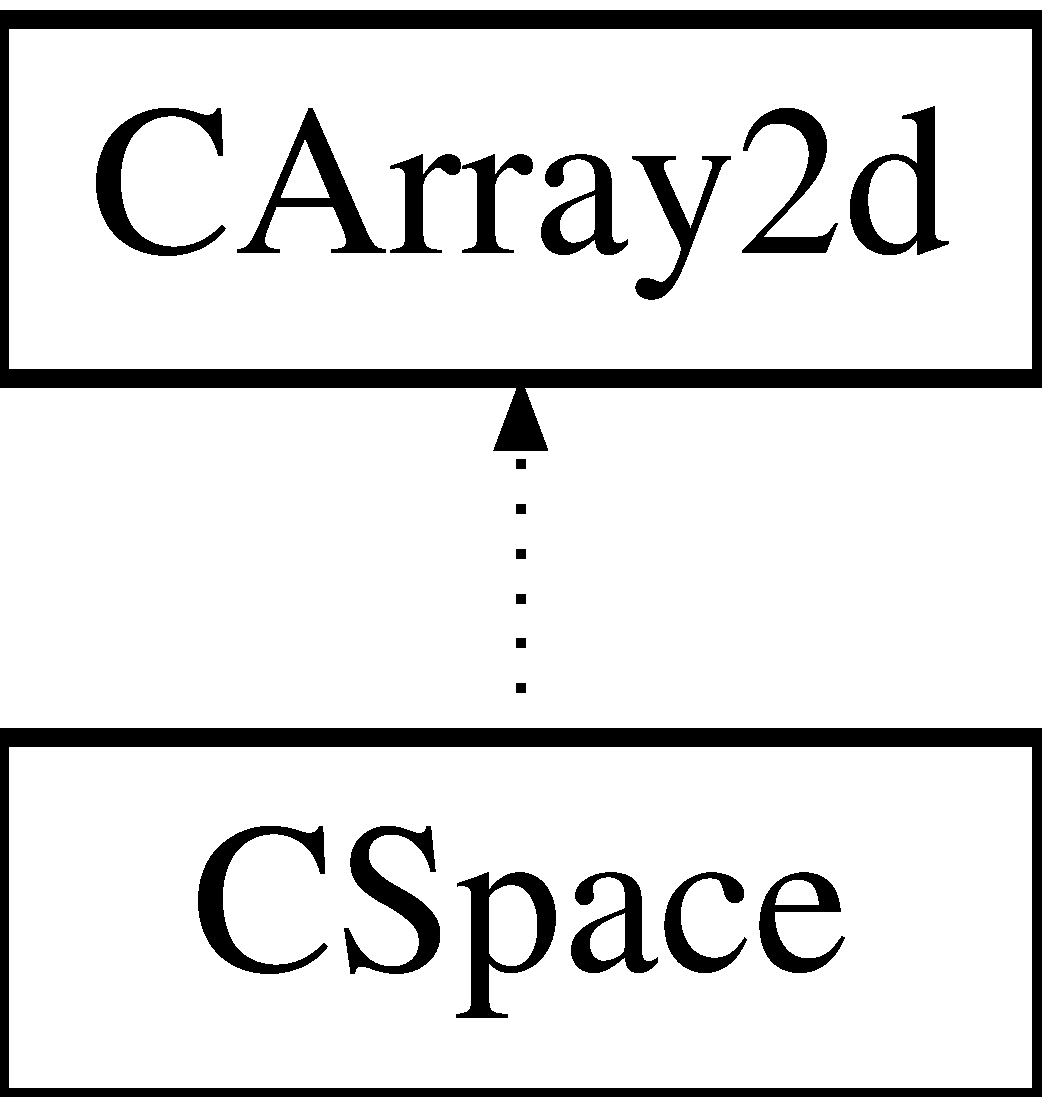
\includegraphics[height=2cm]{classCArray2d}
\end{center}
\end{figure}
\subsection*{Public Member Functions}
\begin{DoxyCompactItemize}
\item 
\hyperlink{classCArray2d_a89adc38a3b0859b819fee52cc054f519}{CArray2d} (int sizeX=SPACE\_\-SIZE\_\-X\_\-DEFAULT, int sizeY=SPACE\_\-SIZE\_\-Y\_\-DEFAULT, BYTE stateDef=CELL\_\-STATE\_\-EMPTY, \hyperlink{classCConfigCore}{CConfigCore} $\ast$pCC=NULL)
\item 
\hyperlink{classCArray2d_a166233a87063ef3ae7d510c8f055df56}{$\sim$CArray2d} ()
\item 
BYTE \hyperlink{classCArray2d_a4d823e1efbdf408cf6960ccd9a40f651}{operator()} (int posX, int posY) const 
\item 
BYTE \& \hyperlink{classCArray2d_aa2e06bfd438eff2979d51c87b561343b}{operator()} (int posX, int posY)
\item 
\hyperlink{classCArray2d}{CArray2d} \& \hyperlink{classCArray2d_aed5c505b790e7b4ea06bf46ef67065f8}{operator=} (const \hyperlink{classCArray2d}{CArray2d} \&rSide)
\item 
int \hyperlink{classCArray2d_a7cfeb98b3112d1e147464a7ec2374579}{GetWidth} ()
\item 
int \hyperlink{classCArray2d_ae019e1beca716a4ea7d368e342fe23a1}{GetHeight} ()
\item 
int \hyperlink{classCArray2d_a021336ae61eb605e5d534722259d3c62}{GetWidth} () const 
\item 
int \hyperlink{classCArray2d_afbfa71015584fcb399c6fde2fa9be1b0}{GetHeight} () const 
\item 
void \hyperlink{classCArray2d_a3b4fc6d5c1536af5e6aead66ee7259eb}{ClearArray} ()
\item 
void \hyperlink{classCArray2d_a7171786b38896bf4bc52261daae3dde0}{ClearArray} (BYTE newDefState)
\item 
int \hyperlink{classCArray2d_afee234adb0190a1d8f3841f75a295e26}{GetErrorFlag} ()
\end{DoxyCompactItemize}
\subsection*{Private Member Functions}
\begin{DoxyCompactItemize}
\item 
int \hyperlink{classCArray2d_ad7566b350c9840af12641ca9385aa352}{AllocMemory} ()
\item 
int \hyperlink{classCArray2d_a83f5fbefa605a6f1875d084f4f2a3600}{DeleteMemory} ()
\item 
int \hyperlink{classCArray2d_aa568ff144541b03023e1afc3c8fe9cba}{InitArray} (int sizeX, int sizeY)
\end{DoxyCompactItemize}
\subsection*{Private Attributes}
\begin{DoxyCompactItemize}
\item 
\hypertarget{classCArray2d_ab93193625b5110ea20017f82c3a1d426}{
int \hyperlink{classCArray2d_ab93193625b5110ea20017f82c3a1d426}{iSizeX}}
\label{classCArray2d_ab93193625b5110ea20017f82c3a1d426}

\begin{DoxyCompactList}\small\item\em array width \item\end{DoxyCompactList}\item 
\hypertarget{classCArray2d_acdb219b4bf58bc1fbc0ca992ae3c49a9}{
int \hyperlink{classCArray2d_acdb219b4bf58bc1fbc0ca992ae3c49a9}{iSizeY}}
\label{classCArray2d_acdb219b4bf58bc1fbc0ca992ae3c49a9}

\begin{DoxyCompactList}\small\item\em array height \item\end{DoxyCompactList}\item 
\hypertarget{classCArray2d_a46b3e446b7a34e04474589a31bd32ff3}{
BYTE \hyperlink{classCArray2d_a46b3e446b7a34e04474589a31bd32ff3}{byDefCellState}}
\label{classCArray2d_a46b3e446b7a34e04474589a31bd32ff3}

\begin{DoxyCompactList}\small\item\em cell's default state \item\end{DoxyCompactList}\item 
\hypertarget{classCArray2d_a29b47cb2b01eb6e235d316ec4926955b}{
BYTE \hyperlink{classCArray2d_a29b47cb2b01eb6e235d316ec4926955b}{byErrCellState}}
\label{classCArray2d_a29b47cb2b01eb6e235d316ec4926955b}

\begin{DoxyCompactList}\small\item\em error state \item\end{DoxyCompactList}\item 
\hypertarget{classCArray2d_ac318244ed315c07a5fd3bb470a4e6e6f}{
struct \hyperlink{structstArray}{stArray} $\ast$ \hyperlink{classCArray2d_ac318244ed315c07a5fd3bb470a4e6e6f}{array}}
\label{classCArray2d_ac318244ed315c07a5fd3bb470a4e6e6f}

\begin{DoxyCompactList}\small\item\em pointer to dyn.allocated 2d array \item\end{DoxyCompactList}\item 
\hypertarget{classCArray2d_ae645314b8bd552e6dde20366307e8218}{
\hyperlink{classCConfigCore}{CConfigCore} $\ast$ \hyperlink{classCArray2d_ae645314b8bd552e6dde20366307e8218}{pConfigCoreArray}}
\label{classCArray2d_ae645314b8bd552e6dde20366307e8218}

\begin{DoxyCompactList}\small\item\em pointer to config class \item\end{DoxyCompactList}\item 
\hypertarget{classCArray2d_a3650a21ae3734efd20a575caa28feeda}{
int \hyperlink{classCArray2d_a3650a21ae3734efd20a575caa28feeda}{iErrFlag}}
\label{classCArray2d_a3650a21ae3734efd20a575caa28feeda}

\begin{DoxyCompactList}\small\item\em error flag \item\end{DoxyCompactList}\end{DoxyCompactItemize}


\subsection{Detailed Description}
contains 2d array, which is used as cellular space for CA 

\subsection{Constructor \& Destructor Documentation}
\hypertarget{classCArray2d_a89adc38a3b0859b819fee52cc054f519}{
\index{CArray2d@{CArray2d}!CArray2d@{CArray2d}}
\index{CArray2d@{CArray2d}!CArray2d@{CArray2d}}
\subsubsection[{CArray2d}]{\setlength{\rightskip}{0pt plus 5cm}CArray2d::CArray2d (int {\em sizeX} = {\ttfamily SPACE\_\-SIZE\_\-X\_\-DEFAULT}, \/  int {\em sizeY} = {\ttfamily SPACE\_\-SIZE\_\-Y\_\-DEFAULT}, \/  BYTE {\em stateDef} = {\ttfamily CELL\_\-STATE\_\-EMPTY}, \/  {\bf CConfigCore} $\ast$ {\em pCC} = {\ttfamily NULL})}}
\label{classCArray2d_a89adc38a3b0859b819fee52cc054f519}
class constructor


\begin{DoxyParams}{Parameters}
\item[{\em sizeX}]x-\/dimension of array \item[{\em sizeY}]y-\/dimension of array \item[{\em stateDef}]default state of cell \item[{\em $\ast$pCC}]pointer to config class \end{DoxyParams}
\hypertarget{classCArray2d_a166233a87063ef3ae7d510c8f055df56}{
\index{CArray2d@{CArray2d}!$\sim$CArray2d@{$\sim$CArray2d}}
\index{$\sim$CArray2d@{$\sim$CArray2d}!CArray2d@{CArray2d}}
\subsubsection[{$\sim$CArray2d}]{\setlength{\rightskip}{0pt plus 5cm}CArray2d::$\sim$CArray2d ()}}
\label{classCArray2d_a166233a87063ef3ae7d510c8f055df56}
class destructor 

\subsection{Member Function Documentation}
\hypertarget{classCArray2d_ad7566b350c9840af12641ca9385aa352}{
\index{CArray2d@{CArray2d}!AllocMemory@{AllocMemory}}
\index{AllocMemory@{AllocMemory}!CArray2d@{CArray2d}}
\subsubsection[{AllocMemory}]{\setlength{\rightskip}{0pt plus 5cm}int CArray2d::AllocMemory ()\hspace{0.3cm}{\ttfamily  \mbox{[}private\mbox{]}}}}
\label{classCArray2d_ad7566b350c9840af12641ca9385aa352}
allocates memory for 2d array \hypertarget{classCArray2d_a7171786b38896bf4bc52261daae3dde0}{
\index{CArray2d@{CArray2d}!ClearArray@{ClearArray}}
\index{ClearArray@{ClearArray}!CArray2d@{CArray2d}}
\subsubsection[{ClearArray}]{\setlength{\rightskip}{0pt plus 5cm}void CArray2d::ClearArray (BYTE {\em newDefState})}}
\label{classCArray2d_a7171786b38896bf4bc52261daae3dde0}
clears array -\/ sets all cell to given value


\begin{DoxyParams}{Parameters}
\item[{\em newDefState}]new default state of cells \end{DoxyParams}
\hypertarget{classCArray2d_a3b4fc6d5c1536af5e6aead66ee7259eb}{
\index{CArray2d@{CArray2d}!ClearArray@{ClearArray}}
\index{ClearArray@{ClearArray}!CArray2d@{CArray2d}}
\subsubsection[{ClearArray}]{\setlength{\rightskip}{0pt plus 5cm}void CArray2d::ClearArray ()}}
\label{classCArray2d_a3b4fc6d5c1536af5e6aead66ee7259eb}
clears array -\/ sets all cell to default value \hypertarget{classCArray2d_a83f5fbefa605a6f1875d084f4f2a3600}{
\index{CArray2d@{CArray2d}!DeleteMemory@{DeleteMemory}}
\index{DeleteMemory@{DeleteMemory}!CArray2d@{CArray2d}}
\subsubsection[{DeleteMemory}]{\setlength{\rightskip}{0pt plus 5cm}int CArray2d::DeleteMemory ()\hspace{0.3cm}{\ttfamily  \mbox{[}private\mbox{]}}}}
\label{classCArray2d_a83f5fbefa605a6f1875d084f4f2a3600}
deletes memory of 2d array \hypertarget{classCArray2d_afee234adb0190a1d8f3841f75a295e26}{
\index{CArray2d@{CArray2d}!GetErrorFlag@{GetErrorFlag}}
\index{GetErrorFlag@{GetErrorFlag}!CArray2d@{CArray2d}}
\subsubsection[{GetErrorFlag}]{\setlength{\rightskip}{0pt plus 5cm}int CArray2d::GetErrorFlag ()}}
\label{classCArray2d_afee234adb0190a1d8f3841f75a295e26}
returns error flag 

Reimplemented in \hyperlink{classCSpace_afe1840ea70f14055a39090ceaec9778e}{CSpace}.\hypertarget{classCArray2d_afbfa71015584fcb399c6fde2fa9be1b0}{
\index{CArray2d@{CArray2d}!GetHeight@{GetHeight}}
\index{GetHeight@{GetHeight}!CArray2d@{CArray2d}}
\subsubsection[{GetHeight}]{\setlength{\rightskip}{0pt plus 5cm}int CArray2d::GetHeight () const}}
\label{classCArray2d_afbfa71015584fcb399c6fde2fa9be1b0}
returns height of array \hypertarget{classCArray2d_ae019e1beca716a4ea7d368e342fe23a1}{
\index{CArray2d@{CArray2d}!GetHeight@{GetHeight}}
\index{GetHeight@{GetHeight}!CArray2d@{CArray2d}}
\subsubsection[{GetHeight}]{\setlength{\rightskip}{0pt plus 5cm}int CArray2d::GetHeight ()}}
\label{classCArray2d_ae019e1beca716a4ea7d368e342fe23a1}
returns height of array 

Reimplemented in \hyperlink{classCSpace_a00b9bce5ca8303b7bae59e2ab6ce98be}{CSpace}.\hypertarget{classCArray2d_a021336ae61eb605e5d534722259d3c62}{
\index{CArray2d@{CArray2d}!GetWidth@{GetWidth}}
\index{GetWidth@{GetWidth}!CArray2d@{CArray2d}}
\subsubsection[{GetWidth}]{\setlength{\rightskip}{0pt plus 5cm}int CArray2d::GetWidth () const}}
\label{classCArray2d_a021336ae61eb605e5d534722259d3c62}
returns width of array \hypertarget{classCArray2d_a7cfeb98b3112d1e147464a7ec2374579}{
\index{CArray2d@{CArray2d}!GetWidth@{GetWidth}}
\index{GetWidth@{GetWidth}!CArray2d@{CArray2d}}
\subsubsection[{GetWidth}]{\setlength{\rightskip}{0pt plus 5cm}int CArray2d::GetWidth ()}}
\label{classCArray2d_a7cfeb98b3112d1e147464a7ec2374579}
returns width of array 

Reimplemented in \hyperlink{classCSpace_a0358e524cecae683cfbcf526ea99d818}{CSpace}.\hypertarget{classCArray2d_aa568ff144541b03023e1afc3c8fe9cba}{
\index{CArray2d@{CArray2d}!InitArray@{InitArray}}
\index{InitArray@{InitArray}!CArray2d@{CArray2d}}
\subsubsection[{InitArray}]{\setlength{\rightskip}{0pt plus 5cm}int CArray2d::InitArray (int {\em sizeX}, \/  int {\em sizeY})\hspace{0.3cm}{\ttfamily  \mbox{[}private\mbox{]}}}}
\label{classCArray2d_aa568ff144541b03023e1afc3c8fe9cba}
array init -\/ checking sizes of axes \hypertarget{classCArray2d_aa2e06bfd438eff2979d51c87b561343b}{
\index{CArray2d@{CArray2d}!operator()@{operator()}}
\index{operator()@{operator()}!CArray2d@{CArray2d}}
\subsubsection[{operator()}]{\setlength{\rightskip}{0pt plus 5cm}BYTE \& CArray2d::operator() (int {\em posX}, \/  int {\em posY})}}
\label{classCArray2d_aa2e06bfd438eff2979d51c87b561343b}
returns reference to element at given coordinates


\begin{DoxyParams}{Parameters}
\item[{\em posX}]position on x-\/axes \item[{\em posY}]position on y-\/axes \end{DoxyParams}
\hypertarget{classCArray2d_a4d823e1efbdf408cf6960ccd9a40f651}{
\index{CArray2d@{CArray2d}!operator()@{operator()}}
\index{operator()@{operator()}!CArray2d@{CArray2d}}
\subsubsection[{operator()}]{\setlength{\rightskip}{0pt plus 5cm}BYTE CArray2d::operator() (int {\em posX}, \/  int {\em posY}) const}}
\label{classCArray2d_a4d823e1efbdf408cf6960ccd9a40f651}
returns element from given coordinates


\begin{DoxyParams}{Parameters}
\item[{\em posX}]position on x-\/axes \item[{\em posY}]position on y-\/axes \end{DoxyParams}
\hypertarget{classCArray2d_aed5c505b790e7b4ea06bf46ef67065f8}{
\index{CArray2d@{CArray2d}!operator=@{operator=}}
\index{operator=@{operator=}!CArray2d@{CArray2d}}
\subsubsection[{operator=}]{\setlength{\rightskip}{0pt plus 5cm}{\bf CArray2d} \& CArray2d::operator= (const {\bf CArray2d} \& {\em rSide})}}
\label{classCArray2d_aed5c505b790e7b4ea06bf46ef67065f8}
copies one array into another


\begin{DoxyParams}{Parameters}
\item[{\em \&rSide}]reference to class on right side of '=' \end{DoxyParams}


The documentation for this class was generated from the following files:\begin{DoxyCompactItemize}
\item 
Array2d.h\item 
Array2d.cpp\end{DoxyCompactItemize}

\hypertarget{classCCellularAutomata}{
\section{CCellularAutomata Class Reference}
\label{classCCellularAutomata}\index{CCellularAutomata@{CCellularAutomata}}
}


{\ttfamily \#include $<$CellularAutomata.h$>$}\subsection*{Public Member Functions}
\begin{DoxyCompactItemize}
\item 
\hyperlink{classCCellularAutomata_a655184244b0dfb0fc760c8456c37544e}{CCellularAutomata} (\hyperlink{classCConfigCore}{CConfigCore} $\ast$configCore)
\item 
\hyperlink{classCCellularAutomata_aea01c28581d9683737ce36f38c1ac7f5}{$\sim$CCellularAutomata} ()
\item 
void \hyperlink{classCCellularAutomata_af5cdf03c18ba644e345daab376d210f9}{Step} ()
\item 
void \hyperlink{classCCellularAutomata_a5ec2f3241ecacde9250f140b4d93470c}{StepGoL} ()
\item 
void \hyperlink{classCCellularAutomata_ade214ca0b4f554561de04ad477ae37c7}{InitMemory} ()
\item 
void \hyperlink{classCCellularAutomata_ab1df4fc7a5d32eed82d62e99aaec3f1f}{InitSpace} ()
\item 
void \hyperlink{classCCellularAutomata_ade3b43b44d2e2cc448d5c896ae389957}{ReInit} ()
\item 
\hyperlink{classCRulesTable}{CRulesTable} $\ast$ \hyperlink{classCCellularAutomata_a4bdd830043f0e68a762e5da35d0a092a}{GetRulesTable} ()
\begin{DoxyCompactList}\small\item\em ============================================================== \item\end{DoxyCompactList}\item 
void \hyperlink{classCCellularAutomata_a0ba78441e4834407637d70e5ccf98e79}{SetConfigCore} (\hyperlink{classCConfigCore}{CConfigCore} $\ast$ccc)
\item 
\hyperlink{classCSpace}{CSpace} $\ast$ \hyperlink{classCCellularAutomata_a811ef34c9aac8e7c9d9dffc1cf69b959}{GetSpace} ()
\item 
\hyperlink{classCSpace}{CSpace} $\ast$ \hyperlink{classCCellularAutomata_ab11e05819885f5ce5450d5ea10d073d8}{GetInitSpace} ()
\item 
int \hyperlink{classCCellularAutomata_a4de26e7af894bb68740fb88e5e84bde7}{GetStepsDone} ()
\item 
int \hyperlink{classCCellularAutomata_ad0e09d8cc86ac519ccb237c77d4a88cc}{GetErrorFlag} ()
\item 
bool \hyperlink{classCCellularAutomata_a1818fe798c2bbcd3028b6dbe6f671965}{IsInitDone} ()
\end{DoxyCompactItemize}
\subsection*{Private Member Functions}
\begin{DoxyCompactItemize}
\item 
void \hyperlink{classCCellularAutomata_a41cd53509e1fa773fd6a5ea08b08a2c1}{DeleteSpace} ()
\item 
void \hyperlink{classCCellularAutomata_a8b1286ff6ab0aa60b2e407cb09389cd8}{DeleteSpaceInit} ()
\item 
void \hyperlink{classCCellularAutomata_a02b47aed358ce08d72171ef555bbe2d3}{GoL} ()
\end{DoxyCompactItemize}
\subsection*{Private Attributes}
\begin{DoxyCompactItemize}
\item 
\hypertarget{classCCellularAutomata_a856d50a387aaa5b24b0f982c59704534}{
\hyperlink{classCRulesTable}{CRulesTable} \hyperlink{classCCellularAutomata_a856d50a387aaa5b24b0f982c59704534}{rules}}
\label{classCCellularAutomata_a856d50a387aaa5b24b0f982c59704534}

\begin{DoxyCompactList}\small\item\em instance of rules table \item\end{DoxyCompactList}\item 
\hypertarget{classCCellularAutomata_ae38dbd5f4ff0a7ccef1befc45a8fc8d2}{
\hyperlink{classCTFunction}{CTFunction} \hyperlink{classCCellularAutomata_ae38dbd5f4ff0a7ccef1befc45a8fc8d2}{tfunction}}
\label{classCCellularAutomata_ae38dbd5f4ff0a7ccef1befc45a8fc8d2}

\begin{DoxyCompactList}\small\item\em instance of transition function \item\end{DoxyCompactList}\item 
\hypertarget{classCCellularAutomata_ac5ad3726d78ae250825ae79eb6c226fc}{
\hyperlink{classCConfigCore}{CConfigCore} $\ast$ \hyperlink{classCCellularAutomata_ac5ad3726d78ae250825ae79eb6c226fc}{pConfigCore}}
\label{classCCellularAutomata_ac5ad3726d78ae250825ae79eb6c226fc}

\begin{DoxyCompactList}\small\item\em pointer to config class \item\end{DoxyCompactList}\item 
\hypertarget{classCCellularAutomata_abe77b69b74343937505dfc8baf7573f4}{
\hyperlink{classCSpace}{CSpace} $\ast$ \hyperlink{classCCellularAutomata_abe77b69b74343937505dfc8baf7573f4}{spaceInit}}
\label{classCCellularAutomata_abe77b69b74343937505dfc8baf7573f4}

\begin{DoxyCompactList}\small\item\em init space -\/ this class containes init ca space definated by user \item\end{DoxyCompactList}\item 
\hypertarget{classCCellularAutomata_a8d83846d9887075192d5f1d78a55e6d5}{
\hyperlink{classCSpace}{CSpace} $\ast$ \hyperlink{classCCellularAutomata_a8d83846d9887075192d5f1d78a55e6d5}{spaceAct}}
\label{classCCellularAutomata_a8d83846d9887075192d5f1d78a55e6d5}

\begin{DoxyCompactList}\small\item\em sa space in actual step of computation \item\end{DoxyCompactList}\item 
\hypertarget{classCCellularAutomata_ad47abe7b72446b455913196ef3ad7b55}{
\hyperlink{classCSpace}{CSpace} $\ast$ \hyperlink{classCCellularAutomata_ad47abe7b72446b455913196ef3ad7b55}{spaceTmp}}
\label{classCCellularAutomata_ad47abe7b72446b455913196ef3ad7b55}

\begin{DoxyCompactList}\small\item\em tmp space is used for saving next step result \item\end{DoxyCompactList}\item 
\hypertarget{classCCellularAutomata_af5d63ae730ccbe73cce038562f9a73aa}{
\hyperlink{classCSpace}{CSpace} $\ast$ \hyperlink{classCCellularAutomata_af5d63ae730ccbe73cce038562f9a73aa}{spaceTmpX}}
\label{classCCellularAutomata_af5d63ae730ccbe73cce038562f9a73aa}

\begin{DoxyCompactList}\small\item\em pointer used for switching pointers between act and tmp instances \item\end{DoxyCompactList}\item 
\hypertarget{classCCellularAutomata_ac218781cb45b36af4d7de0ea4676c0f3}{
unsigned int \hyperlink{classCCellularAutomata_ac218781cb45b36af4d7de0ea4676c0f3}{iStepsDone}}
\label{classCCellularAutomata_ac218781cb45b36af4d7de0ea4676c0f3}

\begin{DoxyCompactList}\small\item\em number of steps done \item\end{DoxyCompactList}\item 
\hypertarget{classCCellularAutomata_a14ce0fe077d51a9e7234d9dfc02bda14}{
bool \hyperlink{classCCellularAutomata_a14ce0fe077d51a9e7234d9dfc02bda14}{bInitDone}}
\label{classCCellularAutomata_a14ce0fe077d51a9e7234d9dfc02bda14}

\begin{DoxyCompactList}\small\item\em is init done? \item\end{DoxyCompactList}\item 
\hypertarget{classCCellularAutomata_a3c86a7f73e2c54eb2ee34076948602e9}{
int \hyperlink{classCCellularAutomata_a3c86a7f73e2c54eb2ee34076948602e9}{iErrFlag}}
\label{classCCellularAutomata_a3c86a7f73e2c54eb2ee34076948602e9}

\begin{DoxyCompactList}\small\item\em error flag \item\end{DoxyCompactList}\end{DoxyCompactItemize}


\subsection{Detailed Description}
main class of cellular automaton this class creates instances of ca space and manages ca computations for computations themself is used class \hyperlink{classCTFunction}{CTFunction}, which calculates index to genome (at this index is gene of BYTE data type which represents value of cell in next step), genome itself is mapped into instance of TRulesTable 

\subsection{Constructor \& Destructor Documentation}
\hypertarget{classCCellularAutomata_a655184244b0dfb0fc760c8456c37544e}{
\index{CCellularAutomata@{CCellularAutomata}!CCellularAutomata@{CCellularAutomata}}
\index{CCellularAutomata@{CCellularAutomata}!CCellularAutomata@{CCellularAutomata}}
\subsubsection[{CCellularAutomata}]{\setlength{\rightskip}{0pt plus 5cm}CCellularAutomata::CCellularAutomata ({\bf CConfigCore} $\ast$ {\em configCore})}}
\label{classCCellularAutomata_a655184244b0dfb0fc760c8456c37544e}
class constructor


\begin{DoxyParams}{Parameters}
\item[{\em $\ast$configCore}]pointer to config class \end{DoxyParams}
\hypertarget{classCCellularAutomata_aea01c28581d9683737ce36f38c1ac7f5}{
\index{CCellularAutomata@{CCellularAutomata}!$\sim$CCellularAutomata@{$\sim$CCellularAutomata}}
\index{$\sim$CCellularAutomata@{$\sim$CCellularAutomata}!CCellularAutomata@{CCellularAutomata}}
\subsubsection[{$\sim$CCellularAutomata}]{\setlength{\rightskip}{0pt plus 5cm}CCellularAutomata::$\sim$CCellularAutomata ()}}
\label{classCCellularAutomata_aea01c28581d9683737ce36f38c1ac7f5}
class destructor 

\subsection{Member Function Documentation}
\hypertarget{classCCellularAutomata_a41cd53509e1fa773fd6a5ea08b08a2c1}{
\index{CCellularAutomata@{CCellularAutomata}!DeleteSpace@{DeleteSpace}}
\index{DeleteSpace@{DeleteSpace}!CCellularAutomata@{CCellularAutomata}}
\subsubsection[{DeleteSpace}]{\setlength{\rightskip}{0pt plus 5cm}void CCellularAutomata::DeleteSpace ()\hspace{0.3cm}{\ttfamily  \mbox{[}private\mbox{]}}}}
\label{classCCellularAutomata_a41cd53509e1fa773fd6a5ea08b08a2c1}
deletes actual and tmp ca spaces \hypertarget{classCCellularAutomata_a8b1286ff6ab0aa60b2e407cb09389cd8}{
\index{CCellularAutomata@{CCellularAutomata}!DeleteSpaceInit@{DeleteSpaceInit}}
\index{DeleteSpaceInit@{DeleteSpaceInit}!CCellularAutomata@{CCellularAutomata}}
\subsubsection[{DeleteSpaceInit}]{\setlength{\rightskip}{0pt plus 5cm}void CCellularAutomata::DeleteSpaceInit ()\hspace{0.3cm}{\ttfamily  \mbox{[}private\mbox{]}}}}
\label{classCCellularAutomata_a8b1286ff6ab0aa60b2e407cb09389cd8}
deletes init ca space \hypertarget{classCCellularAutomata_ad0e09d8cc86ac519ccb237c77d4a88cc}{
\index{CCellularAutomata@{CCellularAutomata}!GetErrorFlag@{GetErrorFlag}}
\index{GetErrorFlag@{GetErrorFlag}!CCellularAutomata@{CCellularAutomata}}
\subsubsection[{GetErrorFlag}]{\setlength{\rightskip}{0pt plus 5cm}int CCellularAutomata::GetErrorFlag ()}}
\label{classCCellularAutomata_ad0e09d8cc86ac519ccb237c77d4a88cc}
return error flag \hypertarget{classCCellularAutomata_ab11e05819885f5ce5450d5ea10d073d8}{
\index{CCellularAutomata@{CCellularAutomata}!GetInitSpace@{GetInitSpace}}
\index{GetInitSpace@{GetInitSpace}!CCellularAutomata@{CCellularAutomata}}
\subsubsection[{GetInitSpace}]{\setlength{\rightskip}{0pt plus 5cm}{\bf CSpace} $\ast$ CCellularAutomata::GetInitSpace ()}}
\label{classCCellularAutomata_ab11e05819885f5ce5450d5ea10d073d8}
returns pointer to init ca space \hypertarget{classCCellularAutomata_a4bdd830043f0e68a762e5da35d0a092a}{
\index{CCellularAutomata@{CCellularAutomata}!GetRulesTable@{GetRulesTable}}
\index{GetRulesTable@{GetRulesTable}!CCellularAutomata@{CCellularAutomata}}
\subsubsection[{GetRulesTable}]{\setlength{\rightskip}{0pt plus 5cm}{\bf CRulesTable} $\ast$ CCellularAutomata::GetRulesTable ()}}
\label{classCCellularAutomata_a4bdd830043f0e68a762e5da35d0a092a}


============================================================== returns pointer to rules table function \hypertarget{classCCellularAutomata_a811ef34c9aac8e7c9d9dffc1cf69b959}{
\index{CCellularAutomata@{CCellularAutomata}!GetSpace@{GetSpace}}
\index{GetSpace@{GetSpace}!CCellularAutomata@{CCellularAutomata}}
\subsubsection[{GetSpace}]{\setlength{\rightskip}{0pt plus 5cm}{\bf CSpace} $\ast$ CCellularAutomata::GetSpace ()}}
\label{classCCellularAutomata_a811ef34c9aac8e7c9d9dffc1cf69b959}
returns pointer to actual CA space \hypertarget{classCCellularAutomata_a4de26e7af894bb68740fb88e5e84bde7}{
\index{CCellularAutomata@{CCellularAutomata}!GetStepsDone@{GetStepsDone}}
\index{GetStepsDone@{GetStepsDone}!CCellularAutomata@{CCellularAutomata}}
\subsubsection[{GetStepsDone}]{\setlength{\rightskip}{0pt plus 5cm}int CCellularAutomata::GetStepsDone ()}}
\label{classCCellularAutomata_a4de26e7af894bb68740fb88e5e84bde7}
return number of done steps \hypertarget{classCCellularAutomata_a02b47aed358ce08d72171ef555bbe2d3}{
\index{CCellularAutomata@{CCellularAutomata}!GoL@{GoL}}
\index{GoL@{GoL}!CCellularAutomata@{CCellularAutomata}}
\subsubsection[{GoL}]{\setlength{\rightskip}{0pt plus 5cm}void CCellularAutomata::GoL ()\hspace{0.3cm}{\ttfamily  \mbox{[}private\mbox{]}}}}
\label{classCCellularAutomata_a02b47aed358ce08d72171ef555bbe2d3}
special funtion for \char`\"{}Game of Life\char`\"{} computations this function does not using chromosomes mapped into transition function \hypertarget{classCCellularAutomata_ade214ca0b4f554561de04ad477ae37c7}{
\index{CCellularAutomata@{CCellularAutomata}!InitMemory@{InitMemory}}
\index{InitMemory@{InitMemory}!CCellularAutomata@{CCellularAutomata}}
\subsubsection[{InitMemory}]{\setlength{\rightskip}{0pt plus 5cm}void CCellularAutomata::InitMemory ()}}
\label{classCCellularAutomata_ade214ca0b4f554561de04ad477ae37c7}
inits memory needed for computation \hypertarget{classCCellularAutomata_ab1df4fc7a5d32eed82d62e99aaec3f1f}{
\index{CCellularAutomata@{CCellularAutomata}!InitSpace@{InitSpace}}
\index{InitSpace@{InitSpace}!CCellularAutomata@{CCellularAutomata}}
\subsubsection[{InitSpace}]{\setlength{\rightskip}{0pt plus 5cm}void CCellularAutomata::InitSpace ()}}
\label{classCCellularAutomata_ab1df4fc7a5d32eed82d62e99aaec3f1f}
init spaces -\/ copies init space into actual space \hypertarget{classCCellularAutomata_a1818fe798c2bbcd3028b6dbe6f671965}{
\index{CCellularAutomata@{CCellularAutomata}!IsInitDone@{IsInitDone}}
\index{IsInitDone@{IsInitDone}!CCellularAutomata@{CCellularAutomata}}
\subsubsection[{IsInitDone}]{\setlength{\rightskip}{0pt plus 5cm}bool CCellularAutomata::IsInitDone ()}}
\label{classCCellularAutomata_a1818fe798c2bbcd3028b6dbe6f671965}
checking if initialization is done \hypertarget{classCCellularAutomata_ade3b43b44d2e2cc448d5c896ae389957}{
\index{CCellularAutomata@{CCellularAutomata}!ReInit@{ReInit}}
\index{ReInit@{ReInit}!CCellularAutomata@{CCellularAutomata}}
\subsubsection[{ReInit}]{\setlength{\rightskip}{0pt plus 5cm}void CCellularAutomata::ReInit ()}}
\label{classCCellularAutomata_ade3b43b44d2e2cc448d5c896ae389957}
reinitialization of CA \hypertarget{classCCellularAutomata_a0ba78441e4834407637d70e5ccf98e79}{
\index{CCellularAutomata@{CCellularAutomata}!SetConfigCore@{SetConfigCore}}
\index{SetConfigCore@{SetConfigCore}!CCellularAutomata@{CCellularAutomata}}
\subsubsection[{SetConfigCore}]{\setlength{\rightskip}{0pt plus 5cm}void CCellularAutomata::SetConfigCore ({\bf CConfigCore} $\ast$ {\em ccc})}}
\label{classCCellularAutomata_a0ba78441e4834407637d70e5ccf98e79}
sets pointer to config class into this class and transition function class


\begin{DoxyParams}{Parameters}
\item[{\em $\ast$ccc}]pointer to config core class \end{DoxyParams}
\hypertarget{classCCellularAutomata_af5cdf03c18ba644e345daab376d210f9}{
\index{CCellularAutomata@{CCellularAutomata}!Step@{Step}}
\index{Step@{Step}!CCellularAutomata@{CCellularAutomata}}
\subsubsection[{Step}]{\setlength{\rightskip}{0pt plus 5cm}void CCellularAutomata::Step ()}}
\label{classCCellularAutomata_af5cdf03c18ba644e345daab376d210f9}
makes one step of ca computation \hypertarget{classCCellularAutomata_a5ec2f3241ecacde9250f140b4d93470c}{
\index{CCellularAutomata@{CCellularAutomata}!StepGoL@{StepGoL}}
\index{StepGoL@{StepGoL}!CCellularAutomata@{CCellularAutomata}}
\subsubsection[{StepGoL}]{\setlength{\rightskip}{0pt plus 5cm}void CCellularAutomata::StepGoL ()}}
\label{classCCellularAutomata_a5ec2f3241ecacde9250f140b4d93470c}
makes one step with special function \hyperlink{classCCellularAutomata_a02b47aed358ce08d72171ef555bbe2d3}{GoL()}, which does not using transition function class 

The documentation for this class was generated from the following files:\begin{DoxyCompactItemize}
\item 
CellularAutomata.h\item 
CellularAutomata.cpp\end{DoxyCompactItemize}

\hypertarget{classCConfigCore}{
\section{CConfigCore Class Reference}
\label{classCConfigCore}\index{CConfigCore@{CConfigCore}}
}
\subsection*{Public Member Functions}
\begin{DoxyCompactItemize}
\item 
\hyperlink{classCConfigCore_a09fdbc421e962fcd0b5ade4db4b21f81}{CConfigCore} ()
\item 
void \hyperlink{classCConfigCore_a698e21d3cc2db7224c8941e3a1505e2a}{SetSpaceType} (int st)
\item 
int \hyperlink{classCConfigCore_a8b06869bfd0a1af47fdd3afc517518d1}{GetSpaceType} ()
\item 
void \hyperlink{classCConfigCore_aed690b7f40faa31694167d5e136e0b54}{SetSpaceSizeX} (int x)
\item 
int \hyperlink{classCConfigCore_aaef0d960846dbe913d073c7aa4634693}{GetSpaceSizeX} ()
\item 
void \hyperlink{classCConfigCore_aada43aac83e4c9ea617f19dd5facc143}{SetSpaceSizeY} (int y)
\item 
int \hyperlink{classCConfigCore_a0a6cce7f05b9c29afa2986059dc0ecaf}{GetSpaceSizeY} ()
\item 
void \hyperlink{classCConfigCore_ac9c465fc1a620c5be2556b02d562b245}{SetStatesCount} (int sc)
\item 
int \hyperlink{classCConfigCore_aff904b7ad2955b6ac7632a967ce73058}{GetStatesCount} ()
\item 
void \hyperlink{classCConfigCore_afde874d899af969cfd1a3cd08dba4234}{SetDefaultState} (int ds)
\item 
BYTE \hyperlink{classCConfigCore_a7623630f4d5737b312f729d312586133}{GetDefaultState} ()
\item 
void \hyperlink{classCConfigCore_ad9e4114043065f44391aa83e73670777}{SetEvolutionRepetitionsCount} (int rc)
\item 
int \hyperlink{classCConfigCore_a44d31a6c355762c899b740c69114d47a}{GetEvolutionRepetitionsCount} ()
\item 
void \hyperlink{classCConfigCore_a80569c4ff831e863896ba20e8847d931}{SetGenerationsCount} (int gc)
\item 
int \hyperlink{classCConfigCore_ae4dbc2fe07b0c5efa776a2e4ccfb47e4}{GetGenerationsCount} ()
\item 
void \hyperlink{classCConfigCore_a5d50ba80b386aa335876254b488911d9}{SetPopulationSize} (int ips)
\item 
int \hyperlink{classCConfigCore_af9e336726122526a8e8e84e45e21ad34}{GetPopulationSize} ()
\item 
void \hyperlink{classCConfigCore_a88d67351c9c94a3a8c95b38163958989}{SetMoveDirection} (int md)
\item 
int \hyperlink{classCConfigCore_add488b09f744e3aa3123099cb6fc0a7f}{GetMoveDirection} ()
\item 
void \hyperlink{classCConfigCore_a58e039e27357b357be539aab708c892e}{SetStepsCountCA} (int sc)
\item 
int \hyperlink{classCConfigCore_a70950ba2f607bbc8e31518f07e831aa5}{GetStepsCountCA} ()
\item 
void \hyperlink{classCConfigCore_a5d89f16000290f977b9bf33cb9f5f0ca}{SetMoveDistance} (int md)
\item 
int \hyperlink{classCConfigCore_abd32b0a6c99afe26029efe8a27590010}{GetMoveDistance} ()
\item 
void \hyperlink{classCConfigCore_aabac109d139d6511fa16e16d768af087}{SetCrossoverProbability} (int cp)
\item 
int \hyperlink{classCConfigCore_a6d6c069032db9af483f3a8c3c32fb0be}{GetCrossoverProbability} ()
\item 
void \hyperlink{classCConfigCore_ab7838b68ad921f40c57528bd1a8f62be}{SetCrossoverCount} (int cc)
\item 
int \hyperlink{classCConfigCore_a655427dab1a00f887346059ad49f4b68}{GetCrossoverCount} ()
\item 
void \hyperlink{classCConfigCore_ab71c04aaf5d5ac97aaa95dde5979e554}{SetMutationProbability} (int mp)
\item 
int \hyperlink{classCConfigCore_a0afa9032f44f906530344f1f92906567}{GetMutationProbability} ()
\item 
void \hyperlink{classCConfigCore_affbb49b26e110a803d9a2a51e14e2a92}{SetMutationCount} (int mc)
\item 
int \hyperlink{classCConfigCore_a8d88cdf520f235a366e4d7f2a5b07e8d}{GetMutationCount} ()
\item 
void \hyperlink{classCConfigCore_abcf39df8c0577d64cd2c447584e26734}{SetGenomeType} (int gt)
\item 
int \hyperlink{classCConfigCore_a10b590690cbe05c9ffd785a82937a657}{GetGenomeType} ()
\item 
void \hyperlink{classCConfigCore_aad6d7e889c24a31f738357c5bb6c11f3}{SetGuiDisplayModeCA} (int dm)
\item 
int \hyperlink{classCConfigCore_af95425d2bb138a4daa6343ab3d8e0389}{GetGuiDisplayModeCA} ()
\item 
void \hyperlink{classCConfigCore_abf0b1f19353a1f0e205b1508754b6582}{SetGuiDisplayModeCATimeout} (int to)
\item 
int \hyperlink{classCConfigCore_ac7b29595aba0f65949b9dd6a4a069c92}{GetGuiDisplayModeCATimeout} ()
\item 
void \hyperlink{classCConfigCore_a22b33872f031fcd3e84c4b085dc5a70c}{SetExportFilePath} (std::string path)
\item 
std::string \hyperlink{classCConfigCore_a37d7199706fa48c52c534a96c9c33591}{GetExportFilePath} ()
\item 
void \hyperlink{classCConfigCore_ab7fb77f1f7774749c04e7d38eb67dbc3}{SetExportFileModeCa} (int mode)
\item 
int \hyperlink{classCConfigCore_a6f7e26303227176cb4a7204104e4a1cb}{GetExportFileModeCa} ()
\item 
void \hyperlink{classCConfigCore_a3f1c3a2faf6edc0f4e77c27d3c8326f3}{SetExportFileModeGa} (int mode)
\item 
int \hyperlink{classCConfigCore_a1537d3260c6d823348ab0edadb780f29}{GetExportFileModeGa} ()
\item 
void \hyperlink{classCConfigCore_a1a7590056fad40d5a2f0cdd2c241ae54}{SetImportGenomeFile} (std::string file)
\item 
std::string \hyperlink{classCConfigCore_a701fd27f77ab5e83d5e050a5bbaadc80}{GetImportGenomeFile} ()
\item 
void \hyperlink{classCConfigCore_a8b868c4f18c8d14fc6132dedce0de6dd}{SetImportGenomeEnabledSimulation} (bool e)
\item 
bool \hyperlink{classCConfigCore_ab5a548edaa135b5a3da90268f9473a9b}{IsImportGenomeEnabledSimulation} ()
\item 
void \hyperlink{classCConfigCore_ac73c74f5e53acd83f7b4272991abfe5e}{SetImportGenomeEnabledReevolve} (bool e)
\item 
bool \hyperlink{classCConfigCore_aac380fe0789216e072fc4cb33b8f0397}{IsImportGenomeEnabledReevolve} ()
\item 
void \hyperlink{classCConfigCore_ae001e63023359519bff27ff78ce4b5b1}{SetExportLogCore} (\hyperlink{classCExportLog}{CExportLog} $\ast$ex)
\item 
\hyperlink{classCExportLog}{CExportLog} $\ast$ \hyperlink{classCConfigCore_acefc129bafcc6fb8a22c901b74d0c65a}{GetExportLogCore} ()
\end{DoxyCompactItemize}
\subsection*{Private Attributes}
\begin{DoxyCompactItemize}
\item 
\hypertarget{classCConfigCore_af74296b7a3c402f0f16b4df8138822b7}{
unsigned int \hyperlink{classCConfigCore_af74296b7a3c402f0f16b4df8138822b7}{iSpaceType}}
\label{classCConfigCore_af74296b7a3c402f0f16b4df8138822b7}

\begin{DoxyCompactList}\small\item\em ca space type -\/ lattice or torus \item\end{DoxyCompactList}\item 
\hypertarget{classCConfigCore_a53b19f7ced02fef8a1e9d6e9feb01f89}{
unsigned int \hyperlink{classCConfigCore_a53b19f7ced02fef8a1e9d6e9feb01f89}{iSizeRunArrayX}}
\label{classCConfigCore_a53b19f7ced02fef8a1e9d6e9feb01f89}

\begin{DoxyCompactList}\small\item\em ca space width \item\end{DoxyCompactList}\item 
\hypertarget{classCConfigCore_a7791749b37cb3aa72b87ac8b3039a1f9}{
unsigned int \hyperlink{classCConfigCore_a7791749b37cb3aa72b87ac8b3039a1f9}{iSizeRunArrayY}}
\label{classCConfigCore_a7791749b37cb3aa72b87ac8b3039a1f9}

\begin{DoxyCompactList}\small\item\em ca space height \item\end{DoxyCompactList}\item 
\hypertarget{classCConfigCore_a2c926a1a68840a45d07477ceba2b1462}{
unsigned int \hyperlink{classCConfigCore_a2c926a1a68840a45d07477ceba2b1462}{iStatesCount}}
\label{classCConfigCore_a2c926a1a68840a45d07477ceba2b1462}

\begin{DoxyCompactList}\small\item\em number of states in ca \item\end{DoxyCompactList}\item 
\hypertarget{classCConfigCore_aa7e6429ff16f44030a6d4a8f83c751e2}{
BYTE \hyperlink{classCConfigCore_aa7e6429ff16f44030a6d4a8f83c751e2}{byDefCellState}}
\label{classCConfigCore_aa7e6429ff16f44030a6d4a8f83c751e2}

\begin{DoxyCompactList}\small\item\em default cell state \item\end{DoxyCompactList}\item 
\hypertarget{classCConfigCore_af67c2f947f1532f70db2283cd7f7b414}{
unsigned int \hyperlink{classCConfigCore_af67c2f947f1532f70db2283cd7f7b414}{iRepetitions}}
\label{classCConfigCore_af67c2f947f1532f70db2283cd7f7b414}

\begin{DoxyCompactList}\small\item\em number of independet runs of evolution \item\end{DoxyCompactList}\item 
\hypertarget{classCConfigCore_a0e296dc7801be8e538abd1cf12234f90}{
unsigned int \hyperlink{classCConfigCore_a0e296dc7801be8e538abd1cf12234f90}{iGenCount}}
\label{classCConfigCore_a0e296dc7801be8e538abd1cf12234f90}

\begin{DoxyCompactList}\small\item\em generations count \item\end{DoxyCompactList}\item 
\hypertarget{classCConfigCore_a13b09746af465cac96357a39ada4a4c2}{
unsigned int \hyperlink{classCConfigCore_a13b09746af465cac96357a39ada4a4c2}{iPopulationSize}}
\label{classCConfigCore_a13b09746af465cac96357a39ada4a4c2}

\begin{DoxyCompactList}\small\item\em population size \item\end{DoxyCompactList}\item 
\hypertarget{classCConfigCore_a337aeaa424dac9c70e59762a33983112}{
unsigned int \hyperlink{classCConfigCore_a337aeaa424dac9c70e59762a33983112}{iMoveDir}}
\label{classCConfigCore_a337aeaa424dac9c70e59762a33983112}

\begin{DoxyCompactList}\small\item\em direction of movement \item\end{DoxyCompactList}\item 
\hypertarget{classCConfigCore_a0edd9af2e1964e28191f82c959ff7c50}{
unsigned int \hyperlink{classCConfigCore_a0edd9af2e1964e28191f82c959ff7c50}{iStepsCountCA}}
\label{classCConfigCore_a0edd9af2e1964e28191f82c959ff7c50}

\begin{DoxyCompactList}\small\item\em steps needed to move at distance \item\end{DoxyCompactList}\item 
\hypertarget{classCConfigCore_abb6e00b76d8eeca29fb3fee5f789a708}{
unsigned int \hyperlink{classCConfigCore_abb6e00b76d8eeca29fb3fee5f789a708}{iDistance}}
\label{classCConfigCore_abb6e00b76d8eeca29fb3fee5f789a708}

\begin{DoxyCompactList}\small\item\em distance of movement \item\end{DoxyCompactList}\item 
\hypertarget{classCConfigCore_a9af624f91c1e1a28cc3ef9de7b536fc6}{
unsigned int \hyperlink{classCConfigCore_a9af624f91c1e1a28cc3ef9de7b536fc6}{iCrossoverProb}}
\label{classCConfigCore_a9af624f91c1e1a28cc3ef9de7b536fc6}

\begin{DoxyCompactList}\small\item\em crossover probability \item\end{DoxyCompactList}\item 
\hypertarget{classCConfigCore_a48f46c2cc8781340f3ad6bd9af867538}{
unsigned int \hyperlink{classCConfigCore_a48f46c2cc8781340f3ad6bd9af867538}{iCrossoverCount}}
\label{classCConfigCore_a48f46c2cc8781340f3ad6bd9af867538}

\begin{DoxyCompactList}\small\item\em number of crossovers \item\end{DoxyCompactList}\item 
\hypertarget{classCConfigCore_a29ec5828def8a122ea8503d11d5e7abb}{
unsigned int \hyperlink{classCConfigCore_a29ec5828def8a122ea8503d11d5e7abb}{iMutProb}}
\label{classCConfigCore_a29ec5828def8a122ea8503d11d5e7abb}

\begin{DoxyCompactList}\small\item\em mutation probability \item\end{DoxyCompactList}\item 
\hypertarget{classCConfigCore_ae6f38bed7575cc052a353ef24d317eea}{
unsigned int \hyperlink{classCConfigCore_ae6f38bed7575cc052a353ef24d317eea}{iMutCount}}
\label{classCConfigCore_ae6f38bed7575cc052a353ef24d317eea}

\begin{DoxyCompactList}\small\item\em number of genes which should be mutated \item\end{DoxyCompactList}\item 
\hypertarget{classCConfigCore_a1d25c6b8e6967bcff9264ae2d9d26332}{
unsigned int \hyperlink{classCConfigCore_a1d25c6b8e6967bcff9264ae2d9d26332}{iGenomeType}}
\label{classCConfigCore_a1d25c6b8e6967bcff9264ae2d9d26332}

\begin{DoxyCompactList}\small\item\em genome type: 9-\/neighborhood + 2 states, etc. \item\end{DoxyCompactList}\item 
\hypertarget{classCConfigCore_a0498757f8539176bbe6f98c33f2df285}{
unsigned int \hyperlink{classCConfigCore_a0498757f8539176bbe6f98c33f2df285}{iGuiDisplayModeCa}}
\label{classCConfigCore_a0498757f8539176bbe6f98c33f2df285}

\begin{DoxyCompactList}\small\item\em gui diaplay mode \item\end{DoxyCompactList}\item 
\hypertarget{classCConfigCore_a99d279d84fedd22e1244885779de4cdf}{
unsigned int \hyperlink{classCConfigCore_a99d279d84fedd22e1244885779de4cdf}{iGuiDisplayModeCaTimeout}}
\label{classCConfigCore_a99d279d84fedd22e1244885779de4cdf}

\begin{DoxyCompactList}\small\item\em gui ca animation timeout (between two steps of ca in \char`\"{}Run\char`\"{} mode) \item\end{DoxyCompactList}\item 
\hypertarget{classCConfigCore_a0b84dcc6083a6d1f56245b6e847c5b8d}{
std::string \hyperlink{classCConfigCore_a0b84dcc6083a6d1f56245b6e847c5b8d}{sgExportFilePath}}
\label{classCConfigCore_a0b84dcc6083a6d1f56245b6e847c5b8d}

\begin{DoxyCompactList}\small\item\em path for files for exported \item\end{DoxyCompactList}\item 
\hypertarget{classCConfigCore_ae94d0e50bb1d83b930d5a23be3bb73c8}{
int \hyperlink{classCConfigCore_ae94d0e50bb1d83b930d5a23be3bb73c8}{iExportFileModeCa}}
\label{classCConfigCore_ae94d0e50bb1d83b930d5a23be3bb73c8}

\begin{DoxyCompactList}\small\item\em mode for exporting ca spaces \item\end{DoxyCompactList}\item 
\hypertarget{classCConfigCore_abb8b60e7b7a3b288ec22a7966e3fc1aa}{
int \hyperlink{classCConfigCore_abb8b60e7b7a3b288ec22a7966e3fc1aa}{iExportFileModeGa}}
\label{classCConfigCore_abb8b60e7b7a3b288ec22a7966e3fc1aa}

\begin{DoxyCompactList}\small\item\em mode for exporting ga genomes \item\end{DoxyCompactList}\item 
\hypertarget{classCConfigCore_abb1f2a7e873eafd18da24a3c285f96f2}{
std::string \hyperlink{classCConfigCore_abb1f2a7e873eafd18da24a3c285f96f2}{sgImportFileGenome}}
\label{classCConfigCore_abb1f2a7e873eafd18da24a3c285f96f2}

\begin{DoxyCompactList}\small\item\em imported genome file path/name \item\end{DoxyCompactList}\item 
\hypertarget{classCConfigCore_a19e42569fbdaf37b78051b9b6f4c2090}{
bool \hyperlink{classCConfigCore_a19e42569fbdaf37b78051b9b6f4c2090}{bImportFileEnabledSimulation}}
\label{classCConfigCore_a19e42569fbdaf37b78051b9b6f4c2090}

\begin{DoxyCompactList}\small\item\em use imported genome just for ca simulation running \item\end{DoxyCompactList}\item 
\hypertarget{classCConfigCore_a6040713bcfc41a177139ddd0c3ba17d5}{
bool \hyperlink{classCConfigCore_a6040713bcfc41a177139ddd0c3ba17d5}{bImportFileEnabledReevolve}}
\label{classCConfigCore_a6040713bcfc41a177139ddd0c3ba17d5}

\begin{DoxyCompactList}\small\item\em re-\/evolve imported genome \item\end{DoxyCompactList}\item 
\hypertarget{classCConfigCore_ab5dc25bcfe91941e290a2c9537d3e585}{
\hyperlink{classCExportLog}{CExportLog} $\ast$ \hyperlink{classCConfigCore_ab5dc25bcfe91941e290a2c9537d3e585}{pExportLogCore}}
\label{classCConfigCore_ab5dc25bcfe91941e290a2c9537d3e585}

\begin{DoxyCompactList}\small\item\em pointer to instance of export log file class created in \hyperlink{classCThreadCore}{CThreadCore} \item\end{DoxyCompactList}\end{DoxyCompactItemize}


\subsection{Constructor \& Destructor Documentation}
\hypertarget{classCConfigCore_a09fdbc421e962fcd0b5ade4db4b21f81}{
\index{CConfigCore@{CConfigCore}!CConfigCore@{CConfigCore}}
\index{CConfigCore@{CConfigCore}!CConfigCore@{CConfigCore}}
\subsubsection[{CConfigCore}]{\setlength{\rightskip}{0pt plus 5cm}CConfigCore::CConfigCore ()}}
\label{classCConfigCore_a09fdbc421e962fcd0b5ade4db4b21f81}
class constructor initializes vars to default values 

\subsection{Member Function Documentation}
\hypertarget{classCConfigCore_a655427dab1a00f887346059ad49f4b68}{
\index{CConfigCore@{CConfigCore}!GetCrossoverCount@{GetCrossoverCount}}
\index{GetCrossoverCount@{GetCrossoverCount}!CConfigCore@{CConfigCore}}
\subsubsection[{GetCrossoverCount}]{\setlength{\rightskip}{0pt plus 5cm}int CConfigCore::GetCrossoverCount ()}}
\label{classCConfigCore_a655427dab1a00f887346059ad49f4b68}
returns count of crossovers between two genomes \hypertarget{classCConfigCore_a6d6c069032db9af483f3a8c3c32fb0be}{
\index{CConfigCore@{CConfigCore}!GetCrossoverProbability@{GetCrossoverProbability}}
\index{GetCrossoverProbability@{GetCrossoverProbability}!CConfigCore@{CConfigCore}}
\subsubsection[{GetCrossoverProbability}]{\setlength{\rightskip}{0pt plus 5cm}int CConfigCore::GetCrossoverProbability ()}}
\label{classCConfigCore_a6d6c069032db9af483f3a8c3c32fb0be}
returns crossover probability \hypertarget{classCConfigCore_a7623630f4d5737b312f729d312586133}{
\index{CConfigCore@{CConfigCore}!GetDefaultState@{GetDefaultState}}
\index{GetDefaultState@{GetDefaultState}!CConfigCore@{CConfigCore}}
\subsubsection[{GetDefaultState}]{\setlength{\rightskip}{0pt plus 5cm}BYTE CConfigCore::GetDefaultState ()}}
\label{classCConfigCore_a7623630f4d5737b312f729d312586133}
returns ca default state \hypertarget{classCConfigCore_a44d31a6c355762c899b740c69114d47a}{
\index{CConfigCore@{CConfigCore}!GetEvolutionRepetitionsCount@{GetEvolutionRepetitionsCount}}
\index{GetEvolutionRepetitionsCount@{GetEvolutionRepetitionsCount}!CConfigCore@{CConfigCore}}
\subsubsection[{GetEvolutionRepetitionsCount}]{\setlength{\rightskip}{0pt plus 5cm}int CConfigCore::GetEvolutionRepetitionsCount ()}}
\label{classCConfigCore_a44d31a6c355762c899b740c69114d47a}
returns count of independent runs of ca \hypertarget{classCConfigCore_a6f7e26303227176cb4a7204104e4a1cb}{
\index{CConfigCore@{CConfigCore}!GetExportFileModeCa@{GetExportFileModeCa}}
\index{GetExportFileModeCa@{GetExportFileModeCa}!CConfigCore@{CConfigCore}}
\subsubsection[{GetExportFileModeCa}]{\setlength{\rightskip}{0pt plus 5cm}int CConfigCore::GetExportFileModeCa ()}}
\label{classCConfigCore_a6f7e26303227176cb4a7204104e4a1cb}
returns ca export mode \hypertarget{classCConfigCore_a1537d3260c6d823348ab0edadb780f29}{
\index{CConfigCore@{CConfigCore}!GetExportFileModeGa@{GetExportFileModeGa}}
\index{GetExportFileModeGa@{GetExportFileModeGa}!CConfigCore@{CConfigCore}}
\subsubsection[{GetExportFileModeGa}]{\setlength{\rightskip}{0pt plus 5cm}int CConfigCore::GetExportFileModeGa ()}}
\label{classCConfigCore_a1537d3260c6d823348ab0edadb780f29}
returns ga export mode \hypertarget{classCConfigCore_a37d7199706fa48c52c534a96c9c33591}{
\index{CConfigCore@{CConfigCore}!GetExportFilePath@{GetExportFilePath}}
\index{GetExportFilePath@{GetExportFilePath}!CConfigCore@{CConfigCore}}
\subsubsection[{GetExportFilePath}]{\setlength{\rightskip}{0pt plus 5cm}std::string CConfigCore::GetExportFilePath ()}}
\label{classCConfigCore_a37d7199706fa48c52c534a96c9c33591}
returns path to export folder \hypertarget{classCConfigCore_acefc129bafcc6fb8a22c901b74d0c65a}{
\index{CConfigCore@{CConfigCore}!GetExportLogCore@{GetExportLogCore}}
\index{GetExportLogCore@{GetExportLogCore}!CConfigCore@{CConfigCore}}
\subsubsection[{GetExportLogCore}]{\setlength{\rightskip}{0pt plus 5cm}{\bf CExportLog} $\ast$ CConfigCore::GetExportLogCore ()}}
\label{classCConfigCore_acefc129bafcc6fb8a22c901b74d0c65a}
returns pointer to one and only instance of error log export class \hypertarget{classCConfigCore_ae4dbc2fe07b0c5efa776a2e4ccfb47e4}{
\index{CConfigCore@{CConfigCore}!GetGenerationsCount@{GetGenerationsCount}}
\index{GetGenerationsCount@{GetGenerationsCount}!CConfigCore@{CConfigCore}}
\subsubsection[{GetGenerationsCount}]{\setlength{\rightskip}{0pt plus 5cm}int CConfigCore::GetGenerationsCount ()}}
\label{classCConfigCore_ae4dbc2fe07b0c5efa776a2e4ccfb47e4}
returns generations count \hypertarget{classCConfigCore_a10b590690cbe05c9ffd785a82937a657}{
\index{CConfigCore@{CConfigCore}!GetGenomeType@{GetGenomeType}}
\index{GetGenomeType@{GetGenomeType}!CConfigCore@{CConfigCore}}
\subsubsection[{GetGenomeType}]{\setlength{\rightskip}{0pt plus 5cm}int CConfigCore::GetGenomeType ()}}
\label{classCConfigCore_a10b590690cbe05c9ffd785a82937a657}
returns genome tupe \hypertarget{classCConfigCore_af95425d2bb138a4daa6343ab3d8e0389}{
\index{CConfigCore@{CConfigCore}!GetGuiDisplayModeCA@{GetGuiDisplayModeCA}}
\index{GetGuiDisplayModeCA@{GetGuiDisplayModeCA}!CConfigCore@{CConfigCore}}
\subsubsection[{GetGuiDisplayModeCA}]{\setlength{\rightskip}{0pt plus 5cm}int CConfigCore::GetGuiDisplayModeCA ()}}
\label{classCConfigCore_af95425d2bb138a4daa6343ab3d8e0389}
returns gui display mode for ca \hypertarget{classCConfigCore_ac7b29595aba0f65949b9dd6a4a069c92}{
\index{CConfigCore@{CConfigCore}!GetGuiDisplayModeCATimeout@{GetGuiDisplayModeCATimeout}}
\index{GetGuiDisplayModeCATimeout@{GetGuiDisplayModeCATimeout}!CConfigCore@{CConfigCore}}
\subsubsection[{GetGuiDisplayModeCATimeout}]{\setlength{\rightskip}{0pt plus 5cm}int CConfigCore::GetGuiDisplayModeCATimeout ()}}
\label{classCConfigCore_ac7b29595aba0f65949b9dd6a4a069c92}
returns gui ca animation timeout (between two steps of ca in \char`\"{}Run\char`\"{} mode) \hypertarget{classCConfigCore_a701fd27f77ab5e83d5e050a5bbaadc80}{
\index{CConfigCore@{CConfigCore}!GetImportGenomeFile@{GetImportGenomeFile}}
\index{GetImportGenomeFile@{GetImportGenomeFile}!CConfigCore@{CConfigCore}}
\subsubsection[{GetImportGenomeFile}]{\setlength{\rightskip}{0pt plus 5cm}std::string CConfigCore::GetImportGenomeFile ()}}
\label{classCConfigCore_a701fd27f77ab5e83d5e050a5bbaadc80}
returns imported genome file path/name \hypertarget{classCConfigCore_add488b09f744e3aa3123099cb6fc0a7f}{
\index{CConfigCore@{CConfigCore}!GetMoveDirection@{GetMoveDirection}}
\index{GetMoveDirection@{GetMoveDirection}!CConfigCore@{CConfigCore}}
\subsubsection[{GetMoveDirection}]{\setlength{\rightskip}{0pt plus 5cm}int CConfigCore::GetMoveDirection ()}}
\label{classCConfigCore_add488b09f744e3aa3123099cb6fc0a7f}
returns movement direction \hypertarget{classCConfigCore_abd32b0a6c99afe26029efe8a27590010}{
\index{CConfigCore@{CConfigCore}!GetMoveDistance@{GetMoveDistance}}
\index{GetMoveDistance@{GetMoveDistance}!CConfigCore@{CConfigCore}}
\subsubsection[{GetMoveDistance}]{\setlength{\rightskip}{0pt plus 5cm}int CConfigCore::GetMoveDistance ()}}
\label{classCConfigCore_abd32b0a6c99afe26029efe8a27590010}
returns distance (in cells) to which object should be moved \hypertarget{classCConfigCore_a8d88cdf520f235a366e4d7f2a5b07e8d}{
\index{CConfigCore@{CConfigCore}!GetMutationCount@{GetMutationCount}}
\index{GetMutationCount@{GetMutationCount}!CConfigCore@{CConfigCore}}
\subsubsection[{GetMutationCount}]{\setlength{\rightskip}{0pt plus 5cm}int CConfigCore::GetMutationCount ()}}
\label{classCConfigCore_a8d88cdf520f235a366e4d7f2a5b07e8d}
returns number of genes which should be mutated \hypertarget{classCConfigCore_a0afa9032f44f906530344f1f92906567}{
\index{CConfigCore@{CConfigCore}!GetMutationProbability@{GetMutationProbability}}
\index{GetMutationProbability@{GetMutationProbability}!CConfigCore@{CConfigCore}}
\subsubsection[{GetMutationProbability}]{\setlength{\rightskip}{0pt plus 5cm}int CConfigCore::GetMutationProbability ()}}
\label{classCConfigCore_a0afa9032f44f906530344f1f92906567}
returns mutation probability \hypertarget{classCConfigCore_af9e336726122526a8e8e84e45e21ad34}{
\index{CConfigCore@{CConfigCore}!GetPopulationSize@{GetPopulationSize}}
\index{GetPopulationSize@{GetPopulationSize}!CConfigCore@{CConfigCore}}
\subsubsection[{GetPopulationSize}]{\setlength{\rightskip}{0pt plus 5cm}int CConfigCore::GetPopulationSize ()}}
\label{classCConfigCore_af9e336726122526a8e8e84e45e21ad34}
returns population size \hypertarget{classCConfigCore_aaef0d960846dbe913d073c7aa4634693}{
\index{CConfigCore@{CConfigCore}!GetSpaceSizeX@{GetSpaceSizeX}}
\index{GetSpaceSizeX@{GetSpaceSizeX}!CConfigCore@{CConfigCore}}
\subsubsection[{GetSpaceSizeX}]{\setlength{\rightskip}{0pt plus 5cm}int CConfigCore::GetSpaceSizeX ()}}
\label{classCConfigCore_aaef0d960846dbe913d073c7aa4634693}
returns ca space width \hypertarget{classCConfigCore_a0a6cce7f05b9c29afa2986059dc0ecaf}{
\index{CConfigCore@{CConfigCore}!GetSpaceSizeY@{GetSpaceSizeY}}
\index{GetSpaceSizeY@{GetSpaceSizeY}!CConfigCore@{CConfigCore}}
\subsubsection[{GetSpaceSizeY}]{\setlength{\rightskip}{0pt plus 5cm}int CConfigCore::GetSpaceSizeY ()}}
\label{classCConfigCore_a0a6cce7f05b9c29afa2986059dc0ecaf}
returns ca space height \hypertarget{classCConfigCore_a8b06869bfd0a1af47fdd3afc517518d1}{
\index{CConfigCore@{CConfigCore}!GetSpaceType@{GetSpaceType}}
\index{GetSpaceType@{GetSpaceType}!CConfigCore@{CConfigCore}}
\subsubsection[{GetSpaceType}]{\setlength{\rightskip}{0pt plus 5cm}int CConfigCore::GetSpaceType ()}}
\label{classCConfigCore_a8b06869bfd0a1af47fdd3afc517518d1}
returns ca space type \hypertarget{classCConfigCore_aff904b7ad2955b6ac7632a967ce73058}{
\index{CConfigCore@{CConfigCore}!GetStatesCount@{GetStatesCount}}
\index{GetStatesCount@{GetStatesCount}!CConfigCore@{CConfigCore}}
\subsubsection[{GetStatesCount}]{\setlength{\rightskip}{0pt plus 5cm}int CConfigCore::GetStatesCount ()}}
\label{classCConfigCore_aff904b7ad2955b6ac7632a967ce73058}
returns ca states count \hypertarget{classCConfigCore_a70950ba2f607bbc8e31518f07e831aa5}{
\index{CConfigCore@{CConfigCore}!GetStepsCountCA@{GetStepsCountCA}}
\index{GetStepsCountCA@{GetStepsCountCA}!CConfigCore@{CConfigCore}}
\subsubsection[{GetStepsCountCA}]{\setlength{\rightskip}{0pt plus 5cm}int CConfigCore::GetStepsCountCA ()}}
\label{classCConfigCore_a70950ba2f607bbc8e31518f07e831aa5}
returns number of ca steps needed to move object on given distance \hypertarget{classCConfigCore_aac380fe0789216e072fc4cb33b8f0397}{
\index{CConfigCore@{CConfigCore}!IsImportGenomeEnabledReevolve@{IsImportGenomeEnabledReevolve}}
\index{IsImportGenomeEnabledReevolve@{IsImportGenomeEnabledReevolve}!CConfigCore@{CConfigCore}}
\subsubsection[{IsImportGenomeEnabledReevolve}]{\setlength{\rightskip}{0pt plus 5cm}bool CConfigCore::IsImportGenomeEnabledReevolve ()}}
\label{classCConfigCore_aac380fe0789216e072fc4cb33b8f0397}
returns if imported genome should be re-\/evolved \hypertarget{classCConfigCore_ab5a548edaa135b5a3da90268f9473a9b}{
\index{CConfigCore@{CConfigCore}!IsImportGenomeEnabledSimulation@{IsImportGenomeEnabledSimulation}}
\index{IsImportGenomeEnabledSimulation@{IsImportGenomeEnabledSimulation}!CConfigCore@{CConfigCore}}
\subsubsection[{IsImportGenomeEnabledSimulation}]{\setlength{\rightskip}{0pt plus 5cm}bool CConfigCore::IsImportGenomeEnabledSimulation ()}}
\label{classCConfigCore_ab5a548edaa135b5a3da90268f9473a9b}
returns if genome should be used in ca simulator \hypertarget{classCConfigCore_ab7838b68ad921f40c57528bd1a8f62be}{
\index{CConfigCore@{CConfigCore}!SetCrossoverCount@{SetCrossoverCount}}
\index{SetCrossoverCount@{SetCrossoverCount}!CConfigCore@{CConfigCore}}
\subsubsection[{SetCrossoverCount}]{\setlength{\rightskip}{0pt plus 5cm}void CConfigCore::SetCrossoverCount (int {\em cc})}}
\label{classCConfigCore_ab7838b68ad921f40c57528bd1a8f62be}
sets count of crossovers between two genomes


\begin{DoxyParams}{Parameters}
\item[{\em cc}]crossovers count \end{DoxyParams}
\hypertarget{classCConfigCore_aabac109d139d6511fa16e16d768af087}{
\index{CConfigCore@{CConfigCore}!SetCrossoverProbability@{SetCrossoverProbability}}
\index{SetCrossoverProbability@{SetCrossoverProbability}!CConfigCore@{CConfigCore}}
\subsubsection[{SetCrossoverProbability}]{\setlength{\rightskip}{0pt plus 5cm}void CConfigCore::SetCrossoverProbability (int {\em cp})}}
\label{classCConfigCore_aabac109d139d6511fa16e16d768af087}
sets crossover probability


\begin{DoxyParams}{Parameters}
\item[{\em cp}]crossover probability \end{DoxyParams}
\hypertarget{classCConfigCore_afde874d899af969cfd1a3cd08dba4234}{
\index{CConfigCore@{CConfigCore}!SetDefaultState@{SetDefaultState}}
\index{SetDefaultState@{SetDefaultState}!CConfigCore@{CConfigCore}}
\subsubsection[{SetDefaultState}]{\setlength{\rightskip}{0pt plus 5cm}void CConfigCore::SetDefaultState (int {\em ds})}}
\label{classCConfigCore_afde874d899af969cfd1a3cd08dba4234}
sets ca default state


\begin{DoxyParams}{Parameters}
\item[{\em ds}]ca default state \end{DoxyParams}
\hypertarget{classCConfigCore_ad9e4114043065f44391aa83e73670777}{
\index{CConfigCore@{CConfigCore}!SetEvolutionRepetitionsCount@{SetEvolutionRepetitionsCount}}
\index{SetEvolutionRepetitionsCount@{SetEvolutionRepetitionsCount}!CConfigCore@{CConfigCore}}
\subsubsection[{SetEvolutionRepetitionsCount}]{\setlength{\rightskip}{0pt plus 5cm}void CConfigCore::SetEvolutionRepetitionsCount (int {\em rc})}}
\label{classCConfigCore_ad9e4114043065f44391aa83e73670777}
sets independent runs of evolution


\begin{DoxyParams}{Parameters}
\item[{\em rc}]independent runs count \end{DoxyParams}
\hypertarget{classCConfigCore_ab7fb77f1f7774749c04e7d38eb67dbc3}{
\index{CConfigCore@{CConfigCore}!SetExportFileModeCa@{SetExportFileModeCa}}
\index{SetExportFileModeCa@{SetExportFileModeCa}!CConfigCore@{CConfigCore}}
\subsubsection[{SetExportFileModeCa}]{\setlength{\rightskip}{0pt plus 5cm}void CConfigCore::SetExportFileModeCa (int {\em mode})}}
\label{classCConfigCore_ab7fb77f1f7774749c04e7d38eb67dbc3}
sets ca export mode


\begin{DoxyParams}{Parameters}
\item[{\em mode}]ca export mode \end{DoxyParams}
\hypertarget{classCConfigCore_a3f1c3a2faf6edc0f4e77c27d3c8326f3}{
\index{CConfigCore@{CConfigCore}!SetExportFileModeGa@{SetExportFileModeGa}}
\index{SetExportFileModeGa@{SetExportFileModeGa}!CConfigCore@{CConfigCore}}
\subsubsection[{SetExportFileModeGa}]{\setlength{\rightskip}{0pt plus 5cm}void CConfigCore::SetExportFileModeGa (int {\em mode})}}
\label{classCConfigCore_a3f1c3a2faf6edc0f4e77c27d3c8326f3}
sets ga export mode


\begin{DoxyParams}{Parameters}
\item[{\em mode}]ga export mode \end{DoxyParams}
\hypertarget{classCConfigCore_a22b33872f031fcd3e84c4b085dc5a70c}{
\index{CConfigCore@{CConfigCore}!SetExportFilePath@{SetExportFilePath}}
\index{SetExportFilePath@{SetExportFilePath}!CConfigCore@{CConfigCore}}
\subsubsection[{SetExportFilePath}]{\setlength{\rightskip}{0pt plus 5cm}void CConfigCore::SetExportFilePath (std::string {\em path})}}
\label{classCConfigCore_a22b33872f031fcd3e84c4b085dc5a70c}
sets path to export folder


\begin{DoxyParams}{Parameters}
\item[{\em path}]path to export folder \end{DoxyParams}
\hypertarget{classCConfigCore_ae001e63023359519bff27ff78ce4b5b1}{
\index{CConfigCore@{CConfigCore}!SetExportLogCore@{SetExportLogCore}}
\index{SetExportLogCore@{SetExportLogCore}!CConfigCore@{CConfigCore}}
\subsubsection[{SetExportLogCore}]{\setlength{\rightskip}{0pt plus 5cm}void CConfigCore::SetExportLogCore ({\bf CExportLog} $\ast$ {\em ex})}}
\label{classCConfigCore_ae001e63023359519bff27ff78ce4b5b1}
sets pointer to one and only instance of error log export class


\begin{DoxyParams}{Parameters}
\item[{\em $\ast$ex}]pointer to log class \end{DoxyParams}
\hypertarget{classCConfigCore_a80569c4ff831e863896ba20e8847d931}{
\index{CConfigCore@{CConfigCore}!SetGenerationsCount@{SetGenerationsCount}}
\index{SetGenerationsCount@{SetGenerationsCount}!CConfigCore@{CConfigCore}}
\subsubsection[{SetGenerationsCount}]{\setlength{\rightskip}{0pt plus 5cm}void CConfigCore::SetGenerationsCount (int {\em gc})}}
\label{classCConfigCore_a80569c4ff831e863896ba20e8847d931}
sets generations count


\begin{DoxyParams}{Parameters}
\item[{\em gc}]generations count \end{DoxyParams}
\hypertarget{classCConfigCore_abcf39df8c0577d64cd2c447584e26734}{
\index{CConfigCore@{CConfigCore}!SetGenomeType@{SetGenomeType}}
\index{SetGenomeType@{SetGenomeType}!CConfigCore@{CConfigCore}}
\subsubsection[{SetGenomeType}]{\setlength{\rightskip}{0pt plus 5cm}void CConfigCore::SetGenomeType (int {\em gt})}}
\label{classCConfigCore_abcf39df8c0577d64cd2c447584e26734}
sets genome type


\begin{DoxyParams}{Parameters}
\item[{\em gt}]genome type \end{DoxyParams}
\hypertarget{classCConfigCore_aad6d7e889c24a31f738357c5bb6c11f3}{
\index{CConfigCore@{CConfigCore}!SetGuiDisplayModeCA@{SetGuiDisplayModeCA}}
\index{SetGuiDisplayModeCA@{SetGuiDisplayModeCA}!CConfigCore@{CConfigCore}}
\subsubsection[{SetGuiDisplayModeCA}]{\setlength{\rightskip}{0pt plus 5cm}void CConfigCore::SetGuiDisplayModeCA (int {\em dm})}}
\label{classCConfigCore_aad6d7e889c24a31f738357c5bb6c11f3}
sets gui display mode for ca


\begin{DoxyParams}{Parameters}
\item[{\em dm}]display mode \end{DoxyParams}
\hypertarget{classCConfigCore_abf0b1f19353a1f0e205b1508754b6582}{
\index{CConfigCore@{CConfigCore}!SetGuiDisplayModeCATimeout@{SetGuiDisplayModeCATimeout}}
\index{SetGuiDisplayModeCATimeout@{SetGuiDisplayModeCATimeout}!CConfigCore@{CConfigCore}}
\subsubsection[{SetGuiDisplayModeCATimeout}]{\setlength{\rightskip}{0pt plus 5cm}void CConfigCore::SetGuiDisplayModeCATimeout (int {\em to})}}
\label{classCConfigCore_abf0b1f19353a1f0e205b1508754b6582}
sets gui ca animation timeout (between two steps of ca in \char`\"{}Run\char`\"{} mode)


\begin{DoxyParams}{Parameters}
\item[{\em to}]timeout \end{DoxyParams}
\hypertarget{classCConfigCore_ac73c74f5e53acd83f7b4272991abfe5e}{
\index{CConfigCore@{CConfigCore}!SetImportGenomeEnabledReevolve@{SetImportGenomeEnabledReevolve}}
\index{SetImportGenomeEnabledReevolve@{SetImportGenomeEnabledReevolve}!CConfigCore@{CConfigCore}}
\subsubsection[{SetImportGenomeEnabledReevolve}]{\setlength{\rightskip}{0pt plus 5cm}void CConfigCore::SetImportGenomeEnabledReevolve (bool {\em e})}}
\label{classCConfigCore_ac73c74f5e53acd83f7b4272991abfe5e}
sets if imported genome should be re-\/evolved


\begin{DoxyParams}{Parameters}
\item[{\em e}]enable re-\/evolution \end{DoxyParams}
\hypertarget{classCConfigCore_a8b868c4f18c8d14fc6132dedce0de6dd}{
\index{CConfigCore@{CConfigCore}!SetImportGenomeEnabledSimulation@{SetImportGenomeEnabledSimulation}}
\index{SetImportGenomeEnabledSimulation@{SetImportGenomeEnabledSimulation}!CConfigCore@{CConfigCore}}
\subsubsection[{SetImportGenomeEnabledSimulation}]{\setlength{\rightskip}{0pt plus 5cm}void CConfigCore::SetImportGenomeEnabledSimulation (bool {\em e})}}
\label{classCConfigCore_a8b868c4f18c8d14fc6132dedce0de6dd}
sets if genome should be used in ca simulator


\begin{DoxyParams}{Parameters}
\item[{\em e}]enable usage in ca simulator \end{DoxyParams}
\hypertarget{classCConfigCore_a1a7590056fad40d5a2f0cdd2c241ae54}{
\index{CConfigCore@{CConfigCore}!SetImportGenomeFile@{SetImportGenomeFile}}
\index{SetImportGenomeFile@{SetImportGenomeFile}!CConfigCore@{CConfigCore}}
\subsubsection[{SetImportGenomeFile}]{\setlength{\rightskip}{0pt plus 5cm}void CConfigCore::SetImportGenomeFile (std::string {\em file})}}
\label{classCConfigCore_a1a7590056fad40d5a2f0cdd2c241ae54}
sets imported genome file path/name


\begin{DoxyParams}{Parameters}
\item[{\em file}]imported genome path/name \end{DoxyParams}
\hypertarget{classCConfigCore_a88d67351c9c94a3a8c95b38163958989}{
\index{CConfigCore@{CConfigCore}!SetMoveDirection@{SetMoveDirection}}
\index{SetMoveDirection@{SetMoveDirection}!CConfigCore@{CConfigCore}}
\subsubsection[{SetMoveDirection}]{\setlength{\rightskip}{0pt plus 5cm}void CConfigCore::SetMoveDirection (int {\em md})}}
\label{classCConfigCore_a88d67351c9c94a3a8c95b38163958989}
sets direction of movement


\begin{DoxyParams}{Parameters}
\item[{\em md}]movement direction \end{DoxyParams}
\hypertarget{classCConfigCore_a5d89f16000290f977b9bf33cb9f5f0ca}{
\index{CConfigCore@{CConfigCore}!SetMoveDistance@{SetMoveDistance}}
\index{SetMoveDistance@{SetMoveDistance}!CConfigCore@{CConfigCore}}
\subsubsection[{SetMoveDistance}]{\setlength{\rightskip}{0pt plus 5cm}void CConfigCore::SetMoveDistance (int {\em md})}}
\label{classCConfigCore_a5d89f16000290f977b9bf33cb9f5f0ca}
sets distance (in cells) to which object should be moved


\begin{DoxyParams}{Parameters}
\item[{\em md}]movement distance \end{DoxyParams}
\hypertarget{classCConfigCore_affbb49b26e110a803d9a2a51e14e2a92}{
\index{CConfigCore@{CConfigCore}!SetMutationCount@{SetMutationCount}}
\index{SetMutationCount@{SetMutationCount}!CConfigCore@{CConfigCore}}
\subsubsection[{SetMutationCount}]{\setlength{\rightskip}{0pt plus 5cm}void CConfigCore::SetMutationCount (int {\em mc})}}
\label{classCConfigCore_affbb49b26e110a803d9a2a51e14e2a92}
sets number of genes which should be mutated


\begin{DoxyParams}{Parameters}
\item[{\em mc}]mutated genes count \end{DoxyParams}
\hypertarget{classCConfigCore_ab71c04aaf5d5ac97aaa95dde5979e554}{
\index{CConfigCore@{CConfigCore}!SetMutationProbability@{SetMutationProbability}}
\index{SetMutationProbability@{SetMutationProbability}!CConfigCore@{CConfigCore}}
\subsubsection[{SetMutationProbability}]{\setlength{\rightskip}{0pt plus 5cm}void CConfigCore::SetMutationProbability (int {\em mp})}}
\label{classCConfigCore_ab71c04aaf5d5ac97aaa95dde5979e554}
sets mutation probability


\begin{DoxyParams}{Parameters}
\item[{\em mp}]mutation probability \end{DoxyParams}
\hypertarget{classCConfigCore_a5d50ba80b386aa335876254b488911d9}{
\index{CConfigCore@{CConfigCore}!SetPopulationSize@{SetPopulationSize}}
\index{SetPopulationSize@{SetPopulationSize}!CConfigCore@{CConfigCore}}
\subsubsection[{SetPopulationSize}]{\setlength{\rightskip}{0pt plus 5cm}void CConfigCore::SetPopulationSize (int {\em ips})}}
\label{classCConfigCore_a5d50ba80b386aa335876254b488911d9}
sets population size


\begin{DoxyParams}{Parameters}
\item[{\em ips}]population size \end{DoxyParams}
\hypertarget{classCConfigCore_aed690b7f40faa31694167d5e136e0b54}{
\index{CConfigCore@{CConfigCore}!SetSpaceSizeX@{SetSpaceSizeX}}
\index{SetSpaceSizeX@{SetSpaceSizeX}!CConfigCore@{CConfigCore}}
\subsubsection[{SetSpaceSizeX}]{\setlength{\rightskip}{0pt plus 5cm}void CConfigCore::SetSpaceSizeX (int {\em x})}}
\label{classCConfigCore_aed690b7f40faa31694167d5e136e0b54}
sets ca space width


\begin{DoxyParams}{Parameters}
\item[{\em x}]ca space width \end{DoxyParams}
\hypertarget{classCConfigCore_aada43aac83e4c9ea617f19dd5facc143}{
\index{CConfigCore@{CConfigCore}!SetSpaceSizeY@{SetSpaceSizeY}}
\index{SetSpaceSizeY@{SetSpaceSizeY}!CConfigCore@{CConfigCore}}
\subsubsection[{SetSpaceSizeY}]{\setlength{\rightskip}{0pt plus 5cm}void CConfigCore::SetSpaceSizeY (int {\em y})}}
\label{classCConfigCore_aada43aac83e4c9ea617f19dd5facc143}
sets ca space height


\begin{DoxyParams}{Parameters}
\item[{\em y}]ca space height \end{DoxyParams}
\hypertarget{classCConfigCore_a698e21d3cc2db7224c8941e3a1505e2a}{
\index{CConfigCore@{CConfigCore}!SetSpaceType@{SetSpaceType}}
\index{SetSpaceType@{SetSpaceType}!CConfigCore@{CConfigCore}}
\subsubsection[{SetSpaceType}]{\setlength{\rightskip}{0pt plus 5cm}void CConfigCore::SetSpaceType (int {\em st})}}
\label{classCConfigCore_a698e21d3cc2db7224c8941e3a1505e2a}
sets ca space type


\begin{DoxyParams}{Parameters}
\item[{\em st}]space type \end{DoxyParams}
\hypertarget{classCConfigCore_ac9c465fc1a620c5be2556b02d562b245}{
\index{CConfigCore@{CConfigCore}!SetStatesCount@{SetStatesCount}}
\index{SetStatesCount@{SetStatesCount}!CConfigCore@{CConfigCore}}
\subsubsection[{SetStatesCount}]{\setlength{\rightskip}{0pt plus 5cm}void CConfigCore::SetStatesCount (int {\em sc})}}
\label{classCConfigCore_ac9c465fc1a620c5be2556b02d562b245}
sets ca states count


\begin{DoxyParams}{Parameters}
\item[{\em sc}]ca states count \end{DoxyParams}
\hypertarget{classCConfigCore_a58e039e27357b357be539aab708c892e}{
\index{CConfigCore@{CConfigCore}!SetStepsCountCA@{SetStepsCountCA}}
\index{SetStepsCountCA@{SetStepsCountCA}!CConfigCore@{CConfigCore}}
\subsubsection[{SetStepsCountCA}]{\setlength{\rightskip}{0pt plus 5cm}void CConfigCore::SetStepsCountCA (int {\em sc})}}
\label{classCConfigCore_a58e039e27357b357be539aab708c892e}
sets number of ca steps needed to move object on given distance


\begin{DoxyParams}{Parameters}
\item[{\em sc}]ca steps count \end{DoxyParams}


The documentation for this class was generated from the following files:\begin{DoxyCompactItemize}
\item 
ConfigCore.h\item 
ConfigCore.cpp\end{DoxyCompactItemize}

\hypertarget{classCCore}{
\section{CCore Class Reference}
\label{classCCore}\index{CCore@{CCore}}
}


{\ttfamily \#include $<$Core.h$>$}\subsection*{Signals}
\begin{DoxyCompactItemize}
\item 
\hypertarget{classCCore_a511dd9be6e5a240b61bcab23bc70b322}{
void {\bfseries SignalThreadCoreErr} (int)}
\label{classCCore_a511dd9be6e5a240b61bcab23bc70b322}

\item 
\hypertarget{classCCore_a03dfcdbafa0ec6fd8d608c9b8136dde9}{
void {\bfseries SignalThreadCoreState} (int)}
\label{classCCore_a03dfcdbafa0ec6fd8d608c9b8136dde9}

\item 
\hypertarget{classCCore_a963de9336a447139f8961ed4790d4d8f}{
void {\bfseries SignalNewDataAvailable} ()}
\label{classCCore_a963de9336a447139f8961ed4790d4d8f}

\end{DoxyCompactItemize}
\subsection*{Public Member Functions}
\begin{DoxyCompactItemize}
\item 
\hyperlink{classCCore_a4c7b83e9a0113f0d4eb0c1d86e6d6be7}{CCore} ()
\item 
\hyperlink{classCCore_ad0d1b93c70b1225137690ecb205d49bd}{$\sim$CCore} ()
\item 
void \hyperlink{classCCore_abf803abecd356eca5edff06f3ca6be33}{InitGuiCore} ()
\item 
void \hyperlink{classCCore_ae2e68df5908b34b15106820fde4d4de1}{SetCoreDataExpiration} (bool e)
\item 
void \hyperlink{classCCore_abe4809ea8ec654371e2a412ecbc057ee}{SetSimulationRunning} (bool sr)
\item 
void \hyperlink{classCCore_a799587561a1a236c5f62018fb9c7949e}{SetCaRunTermination} ()
\item 
void \hyperlink{classCCore_ab23cb1edf937f04342dfbbc7c2e1e45a}{StartThreadCore} ()
\item 
bool \hyperlink{classCCore_a9cc1459df131a2757809f13e2af2bf9e}{IsInitDone} ()
\item 
\hyperlink{classCConfigCore}{CConfigCore} $\ast$ \hyperlink{classCCore_a08ea111ccd738ddbc2d29ec3c9ac3443}{GetConfigCore} ()
\item 
\hyperlink{classCSpace}{CSpace} $\ast$ \hyperlink{classCCore_a3eebffde003b3ae3e724136521739e12}{GetSpace} ()
\item 
int \hyperlink{classCCore_a18ce09c76b45dd18a7932c4832f61300}{GetSimCoreGenerationID} ()
\item 
int \hyperlink{classCCore_acad2cd2c8de535f03515281b58c643a6}{GetSimCoreChromosomeID} ()
\item 
int \hyperlink{classCCore_ab1b7b2beb189d420eac4f2af40d883c2}{GetSimCoreAncestorsCount} ()
\item 
int \hyperlink{classCCore_a0de6196e934c38a12fd26875b5e020be}{GetSimCoreFitnessMax} ()
\item 
double \hyperlink{classCCore_a383218fe410dd8425ede9772277e708f}{GetSimCoreFitnessMaxNorm} ()
\item 
int \hyperlink{classCCore_a15daf074c713232f20f772b20098e716}{GetSimCoreDifferentionMin} ()
\item 
int \hyperlink{classCCore_a974f6f52d6cb6362718c7e1a06a767c9}{GetSimCoreFitMaxStepCA} ()
\item 
int \hyperlink{classCCore_a07b0206d4fc75b23bd8da7660d8efc1a}{GetSimCoreSameChromosomesCount} ()
\item 
double \hyperlink{classCCore_aa6634f29c320ed9110ce82eed156b05d}{GetSimCoreSameChromosomesGenerationAvarage} ()
\item 
struct \hyperlink{structstThreadCoreDataGA}{stThreadCoreDataGA} $\ast$ \hyperlink{classCCore_a4ddbbc5f50ff19b2d2b9095792b648a6}{GetSimCoreDataStruct} ()
\item 
int \hyperlink{classCCore_a86ddf9496601836d1dae7432279fd044}{GetErrorFlag} ()
\item 
void \hyperlink{classCCore_ae836cfc9a5b1d30a093cc92c7e0f825b}{ShowDebugConfigCore} ()
\end{DoxyCompactItemize}
\subsection*{Private Slots}
\begin{DoxyCompactItemize}
\item 
void \hyperlink{classCCore_a8da26ce21ea70fb3c31978e6d2fce17e}{ThreadCoreErrorSlot} (int err)
\item 
void \hyperlink{classCCore_a201541672b99640948959c4022f8cda4}{ThreadCoreCheckCoreInitDone} ()
\item 
void \hyperlink{classCCore_a05760021352ea7bdb7304d7d0f2a61eb}{ThreadCoreNewDataAvailable} ()
\item 
void \hyperlink{classCCore_a6b1594d8d1a21121d0db95c5e9a8fabd}{ThreadCoreState} (int s)
\end{DoxyCompactItemize}
\subsection*{Private Attributes}
\begin{DoxyCompactItemize}
\item 
\hypertarget{classCCore_a88cfee1f612c96f3bfede6a20ca5cabd}{
\hyperlink{classCConfigCore}{CConfigCore} \hyperlink{classCCore_a88cfee1f612c96f3bfede6a20ca5cabd}{configCore}}
\label{classCCore_a88cfee1f612c96f3bfede6a20ca5cabd}

\begin{DoxyCompactList}\small\item\em config class \item\end{DoxyCompactList}\item 
\hypertarget{classCCore_a6813b6f89b401a896381a19b04fc509a}{
bool \hyperlink{classCCore_a6813b6f89b401a896381a19b04fc509a}{bCoreDataExpired}}
\label{classCCore_a6813b6f89b401a896381a19b04fc509a}

\begin{DoxyCompactList}\small\item\em are data from this class already displayed in gui? \item\end{DoxyCompactList}\item 
\hypertarget{classCCore_ad0b15abbb2cfc189f6639b1e45041a6d}{
bool \hyperlink{classCCore_ad0b15abbb2cfc189f6639b1e45041a6d}{bSimRunning}}
\label{classCCore_ad0b15abbb2cfc189f6639b1e45041a6d}

\begin{DoxyCompactList}\small\item\em should be evolution running? \item\end{DoxyCompactList}\item 
\hypertarget{classCCore_ad6381478361c75e7be735b6003e45dbd}{
bool \hyperlink{classCCore_ad6381478361c75e7be735b6003e45dbd}{bInitDone}}
\label{classCCore_ad6381478361c75e7be735b6003e45dbd}

\begin{DoxyCompactList}\small\item\em is init done? \item\end{DoxyCompactList}\item 
\hypertarget{classCCore_ad744c98c0206358039db24d89a26e913}{
\hyperlink{classCSpace}{CSpace} $\ast$ \hyperlink{classCCore_ad744c98c0206358039db24d89a26e913}{space}}
\label{classCCore_ad744c98c0206358039db24d89a26e913}

\begin{DoxyCompactList}\small\item\em pointer to ca space class \item\end{DoxyCompactList}\item 
\hypertarget{classCCore_a20b827bf2dafe610e9a5228eb9c6e7ae}{
\hyperlink{classCGenome}{CGenome} $\ast$ \hyperlink{classCCore_a20b827bf2dafe610e9a5228eb9c6e7ae}{genome}}
\label{classCCore_a20b827bf2dafe610e9a5228eb9c6e7ae}

\begin{DoxyCompactList}\small\item\em pointer to genome class \item\end{DoxyCompactList}\item 
\hypertarget{classCCore_a2699b566011cda9d1f69f36c734811ea}{
struct \hyperlink{structstThreadCoreDataGA}{stThreadCoreDataGA} \hyperlink{classCCore_a2699b566011cda9d1f69f36c734811ea}{dataGa}}
\label{classCCore_a2699b566011cda9d1f69f36c734811ea}

\begin{DoxyCompactList}\small\item\em ga data struct used for propagating data from thread core into gui \item\end{DoxyCompactList}\item 
\hypertarget{classCCore_a36b1cf10df7c1d3bd036d69a109ae81b}{
QMutex \hyperlink{classCCore_a36b1cf10df7c1d3bd036d69a109ae81b}{mutexCore}}
\label{classCCore_a36b1cf10df7c1d3bd036d69a109ae81b}

\begin{DoxyCompactList}\small\item\em mutex used for sync gui thread (in which this class runs) with \hyperlink{classCThreadCore}{CThreadCore} thread \item\end{DoxyCompactList}\item 
\hypertarget{classCCore_abf4a4a3ebe49dc69c3c27dd545aa4606}{
QWaitCondition \hyperlink{classCCore_abf4a4a3ebe49dc69c3c27dd545aa4606}{waitCCore}}
\label{classCCore_abf4a4a3ebe49dc69c3c27dd545aa4606}

\begin{DoxyCompactList}\small\item\em wait cond used for sync gui thread (in which this class runs) with \hyperlink{classCThreadCore}{CThreadCore} thread \item\end{DoxyCompactList}\item 
\hypertarget{classCCore_a06fcd7735c831f7dcf1e855313dab8a5}{
\hyperlink{classCThreadCore}{CThreadCore} $\ast$ \hyperlink{classCCore_a06fcd7735c831f7dcf1e855313dab8a5}{threadCore}}
\label{classCCore_a06fcd7735c831f7dcf1e855313dab8a5}

\begin{DoxyCompactList}\small\item\em pointer to instance of thread core class \item\end{DoxyCompactList}\item 
\hypertarget{classCCore_a0d7dcc59aa4cde53f4edc7006e45a2c6}{
int \hyperlink{classCCore_a0d7dcc59aa4cde53f4edc7006e45a2c6}{iErrFlag}}
\label{classCCore_a0d7dcc59aa4cde53f4edc7006e45a2c6}

\begin{DoxyCompactList}\small\item\em error flag \item\end{DoxyCompactList}\end{DoxyCompactItemize}


\subsection{Detailed Description}
this is special class -\/ is used as mediator between gui classes and \hyperlink{classCThreadCore}{CThreadCore} -\/ computation class this class solves thread sync between gui and core core send data from ga and ca to this class, this class then tell gui, that new data arrived and gui then copy this data and displays them, last step is, that gui tells this class, that data are displayed, this class send this info to core, so core will know, that can send new data

this class is created when \char`\"{}Init\char`\"{} button is pressed and deleted when \char`\"{}Delete\char`\"{} button is pressed when init button is pressed, this class creates \hyperlink{classCThreadCore}{CThreadCore} and propagate sync pointers to it when delete is pressed this class kills compute core thread 

\subsection{Constructor \& Destructor Documentation}
\hypertarget{classCCore_a4c7b83e9a0113f0d4eb0c1d86e6d6be7}{
\index{CCore@{CCore}!CCore@{CCore}}
\index{CCore@{CCore}!CCore@{CCore}}
\subsubsection[{CCore}]{\setlength{\rightskip}{0pt plus 5cm}CCore::CCore ()}}
\label{classCCore_a4c7b83e9a0113f0d4eb0c1d86e6d6be7}
class constructor \hypertarget{classCCore_ad0d1b93c70b1225137690ecb205d49bd}{
\index{CCore@{CCore}!$\sim$CCore@{$\sim$CCore}}
\index{$\sim$CCore@{$\sim$CCore}!CCore@{CCore}}
\subsubsection[{$\sim$CCore}]{\setlength{\rightskip}{0pt plus 5cm}CCore::$\sim$CCore ()}}
\label{classCCore_ad0d1b93c70b1225137690ecb205d49bd}
class destructor 

\subsection{Member Function Documentation}
\hypertarget{classCCore_a08ea111ccd738ddbc2d29ec3c9ac3443}{
\index{CCore@{CCore}!GetConfigCore@{GetConfigCore}}
\index{GetConfigCore@{GetConfigCore}!CCore@{CCore}}
\subsubsection[{GetConfigCore}]{\setlength{\rightskip}{0pt plus 5cm}{\bf CConfigCore} $\ast$ CCore::GetConfigCore ()}}
\label{classCCore_a08ea111ccd738ddbc2d29ec3c9ac3443}
return pointer to config class \hypertarget{classCCore_a86ddf9496601836d1dae7432279fd044}{
\index{CCore@{CCore}!GetErrorFlag@{GetErrorFlag}}
\index{GetErrorFlag@{GetErrorFlag}!CCore@{CCore}}
\subsubsection[{GetErrorFlag}]{\setlength{\rightskip}{0pt plus 5cm}int CCore::GetErrorFlag ()}}
\label{classCCore_a86ddf9496601836d1dae7432279fd044}
returns erro flag \hypertarget{classCCore_ab1b7b2beb189d420eac4f2af40d883c2}{
\index{CCore@{CCore}!GetSimCoreAncestorsCount@{GetSimCoreAncestorsCount}}
\index{GetSimCoreAncestorsCount@{GetSimCoreAncestorsCount}!CCore@{CCore}}
\subsubsection[{GetSimCoreAncestorsCount}]{\setlength{\rightskip}{0pt plus 5cm}int CCore::GetSimCoreAncestorsCount ()}}
\label{classCCore_ab1b7b2beb189d420eac4f2af40d883c2}
return ga data -\/ genome's ancestor count \hypertarget{classCCore_acad2cd2c8de535f03515281b58c643a6}{
\index{CCore@{CCore}!GetSimCoreChromosomeID@{GetSimCoreChromosomeID}}
\index{GetSimCoreChromosomeID@{GetSimCoreChromosomeID}!CCore@{CCore}}
\subsubsection[{GetSimCoreChromosomeID}]{\setlength{\rightskip}{0pt plus 5cm}int CCore::GetSimCoreChromosomeID ()}}
\label{classCCore_acad2cd2c8de535f03515281b58c643a6}
return ga data -\/ genome's id \hypertarget{classCCore_a4ddbbc5f50ff19b2d2b9095792b648a6}{
\index{CCore@{CCore}!GetSimCoreDataStruct@{GetSimCoreDataStruct}}
\index{GetSimCoreDataStruct@{GetSimCoreDataStruct}!CCore@{CCore}}
\subsubsection[{GetSimCoreDataStruct}]{\setlength{\rightskip}{0pt plus 5cm}struct {\bf stThreadCoreDataGA} $\ast$ CCore::GetSimCoreDataStruct ()\hspace{0.3cm}{\ttfamily  \mbox{[}read\mbox{]}}}}
\label{classCCore_a4ddbbc5f50ff19b2d2b9095792b648a6}
returns pointer to ga data struct \hypertarget{classCCore_a15daf074c713232f20f772b20098e716}{
\index{CCore@{CCore}!GetSimCoreDifferentionMin@{GetSimCoreDifferentionMin}}
\index{GetSimCoreDifferentionMin@{GetSimCoreDifferentionMin}!CCore@{CCore}}
\subsubsection[{GetSimCoreDifferentionMin}]{\setlength{\rightskip}{0pt plus 5cm}int CCore::GetSimCoreDifferentionMin ()}}
\label{classCCore_a15daf074c713232f20f772b20098e716}
return ga data -\/ genome's minimum differention \hypertarget{classCCore_a974f6f52d6cb6362718c7e1a06a767c9}{
\index{CCore@{CCore}!GetSimCoreFitMaxStepCA@{GetSimCoreFitMaxStepCA}}
\index{GetSimCoreFitMaxStepCA@{GetSimCoreFitMaxStepCA}!CCore@{CCore}}
\subsubsection[{GetSimCoreFitMaxStepCA}]{\setlength{\rightskip}{0pt plus 5cm}int CCore::GetSimCoreFitMaxStepCA ()}}
\label{classCCore_a974f6f52d6cb6362718c7e1a06a767c9}
return ga data -\/ ca step with max fitness \hypertarget{classCCore_a0de6196e934c38a12fd26875b5e020be}{
\index{CCore@{CCore}!GetSimCoreFitnessMax@{GetSimCoreFitnessMax}}
\index{GetSimCoreFitnessMax@{GetSimCoreFitnessMax}!CCore@{CCore}}
\subsubsection[{GetSimCoreFitnessMax}]{\setlength{\rightskip}{0pt plus 5cm}int CCore::GetSimCoreFitnessMax ()}}
\label{classCCore_a0de6196e934c38a12fd26875b5e020be}
return ga data -\/ genome's maximum fitness \hypertarget{classCCore_a383218fe410dd8425ede9772277e708f}{
\index{CCore@{CCore}!GetSimCoreFitnessMaxNorm@{GetSimCoreFitnessMaxNorm}}
\index{GetSimCoreFitnessMaxNorm@{GetSimCoreFitnessMaxNorm}!CCore@{CCore}}
\subsubsection[{GetSimCoreFitnessMaxNorm}]{\setlength{\rightskip}{0pt plus 5cm}double CCore::GetSimCoreFitnessMaxNorm ()}}
\label{classCCore_a383218fe410dd8425ede9772277e708f}
return ga data -\/ genome's maximum fitness \hypertarget{classCCore_a18ce09c76b45dd18a7932c4832f61300}{
\index{CCore@{CCore}!GetSimCoreGenerationID@{GetSimCoreGenerationID}}
\index{GetSimCoreGenerationID@{GetSimCoreGenerationID}!CCore@{CCore}}
\subsubsection[{GetSimCoreGenerationID}]{\setlength{\rightskip}{0pt plus 5cm}int CCore::GetSimCoreGenerationID ()}}
\label{classCCore_a18ce09c76b45dd18a7932c4832f61300}
return ga data -\/ genome's generation id \hypertarget{classCCore_a07b0206d4fc75b23bd8da7660d8efc1a}{
\index{CCore@{CCore}!GetSimCoreSameChromosomesCount@{GetSimCoreSameChromosomesCount}}
\index{GetSimCoreSameChromosomesCount@{GetSimCoreSameChromosomesCount}!CCore@{CCore}}
\subsubsection[{GetSimCoreSameChromosomesCount}]{\setlength{\rightskip}{0pt plus 5cm}int CCore::GetSimCoreSameChromosomesCount ()}}
\label{classCCore_a07b0206d4fc75b23bd8da7660d8efc1a}
return ga data -\/ count of genomes with same fitness \hypertarget{classCCore_aa6634f29c320ed9110ce82eed156b05d}{
\index{CCore@{CCore}!GetSimCoreSameChromosomesGenerationAvarage@{GetSimCoreSameChromosomesGenerationAvarage}}
\index{GetSimCoreSameChromosomesGenerationAvarage@{GetSimCoreSameChromosomesGenerationAvarage}!CCore@{CCore}}
\subsubsection[{GetSimCoreSameChromosomesGenerationAvarage}]{\setlength{\rightskip}{0pt plus 5cm}double CCore::GetSimCoreSameChromosomesGenerationAvarage ()}}
\label{classCCore_aa6634f29c320ed9110ce82eed156b05d}
return ga data -\/ avarage generation of \char`\"{}same\char`\"{} genomes \hypertarget{classCCore_a3eebffde003b3ae3e724136521739e12}{
\index{CCore@{CCore}!GetSpace@{GetSpace}}
\index{GetSpace@{GetSpace}!CCore@{CCore}}
\subsubsection[{GetSpace}]{\setlength{\rightskip}{0pt plus 5cm}{\bf CSpace} $\ast$ CCore::GetSpace ()}}
\label{classCCore_a3eebffde003b3ae3e724136521739e12}
returns pointer to ca space class \hypertarget{classCCore_abf803abecd356eca5edff06f3ca6be33}{
\index{CCore@{CCore}!InitGuiCore@{InitGuiCore}}
\index{InitGuiCore@{InitGuiCore}!CCore@{CCore}}
\subsubsection[{InitGuiCore}]{\setlength{\rightskip}{0pt plus 5cm}void CCore::InitGuiCore ()}}
\label{classCCore_abf803abecd356eca5edff06f3ca6be33}
inits \hyperlink{classCCore}{CCore} and core thread \hyperlink{classCThreadCore}{CThreadCore} propagates dat from this class into \hyperlink{classCThreadCore}{CThreadCore} data from gui are propagated to this class from gui functions \hypertarget{classCCore_a9cc1459df131a2757809f13e2af2bf9e}{
\index{CCore@{CCore}!IsInitDone@{IsInitDone}}
\index{IsInitDone@{IsInitDone}!CCore@{CCore}}
\subsubsection[{IsInitDone}]{\setlength{\rightskip}{0pt plus 5cm}bool CCore::IsInitDone ()}}
\label{classCCore_a9cc1459df131a2757809f13e2af2bf9e}
returns if init is done and ok \hypertarget{classCCore_a799587561a1a236c5f62018fb9c7949e}{
\index{CCore@{CCore}!SetCaRunTermination@{SetCaRunTermination}}
\index{SetCaRunTermination@{SetCaRunTermination}!CCore@{CCore}}
\subsubsection[{SetCaRunTermination}]{\setlength{\rightskip}{0pt plus 5cm}void CCore::SetCaRunTermination ()}}
\label{classCCore_a799587561a1a236c5f62018fb9c7949e}
sets state var shich tells core, that user pressed button \char`\"{}Terminate\char`\"{} for terminating ca simulator \hypertarget{classCCore_ae2e68df5908b34b15106820fde4d4de1}{
\index{CCore@{CCore}!SetCoreDataExpiration@{SetCoreDataExpiration}}
\index{SetCoreDataExpiration@{SetCoreDataExpiration}!CCore@{CCore}}
\subsubsection[{SetCoreDataExpiration}]{\setlength{\rightskip}{0pt plus 5cm}void CCore::SetCoreDataExpiration (bool {\em e})}}
\label{classCCore_ae2e68df5908b34b15106820fde4d4de1}
sets state var, which tells core, that data from this class was already displayed in gui, so new data can be propagete to this class


\begin{DoxyParams}{Parameters}
\item[{\em e}]are core's data expered? (already showed in gui) \end{DoxyParams}
\hypertarget{classCCore_abe4809ea8ec654371e2a412ecbc057ee}{
\index{CCore@{CCore}!SetSimulationRunning@{SetSimulationRunning}}
\index{SetSimulationRunning@{SetSimulationRunning}!CCore@{CCore}}
\subsubsection[{SetSimulationRunning}]{\setlength{\rightskip}{0pt plus 5cm}void CCore::SetSimulationRunning (bool {\em sr})}}
\label{classCCore_abe4809ea8ec654371e2a412ecbc057ee}
sets state var which tells core, that user pressed button \char`\"{}Evolve\char`\"{} so evolution can start


\begin{DoxyParams}{Parameters}
\item[{\em sr}]set ThreadCore thread running state \end{DoxyParams}
\hypertarget{classCCore_ae836cfc9a5b1d30a093cc92c7e0f825b}{
\index{CCore@{CCore}!ShowDebugConfigCore@{ShowDebugConfigCore}}
\index{ShowDebugConfigCore@{ShowDebugConfigCore}!CCore@{CCore}}
\subsubsection[{ShowDebugConfigCore}]{\setlength{\rightskip}{0pt plus 5cm}void CCore::ShowDebugConfigCore ()}}
\label{classCCore_ae836cfc9a5b1d30a093cc92c7e0f825b}
debug INFO \hypertarget{classCCore_ab23cb1edf937f04342dfbbc7c2e1e45a}{
\index{CCore@{CCore}!StartThreadCore@{StartThreadCore}}
\index{StartThreadCore@{StartThreadCore}!CCore@{CCore}}
\subsubsection[{StartThreadCore}]{\setlength{\rightskip}{0pt plus 5cm}void CCore::StartThreadCore ()}}
\label{classCCore_ab23cb1edf937f04342dfbbc7c2e1e45a}
starts \hyperlink{classCThreadCore}{CThreadCore} thread, just init part is compute, then thread waits for \char`\"{}Evolve\char`\"{} button to be pressed \hypertarget{classCCore_a201541672b99640948959c4022f8cda4}{
\index{CCore@{CCore}!ThreadCoreCheckCoreInitDone@{ThreadCoreCheckCoreInitDone}}
\index{ThreadCoreCheckCoreInitDone@{ThreadCoreCheckCoreInitDone}!CCore@{CCore}}
\subsubsection[{ThreadCoreCheckCoreInitDone}]{\setlength{\rightskip}{0pt plus 5cm}void CCore::ThreadCoreCheckCoreInitDone ()\hspace{0.3cm}{\ttfamily  \mbox{[}private, slot\mbox{]}}}}
\label{classCCore_a201541672b99640948959c4022f8cda4}
propagates info about thread core init done into gui \hypertarget{classCCore_a8da26ce21ea70fb3c31978e6d2fce17e}{
\index{CCore@{CCore}!ThreadCoreErrorSlot@{ThreadCoreErrorSlot}}
\index{ThreadCoreErrorSlot@{ThreadCoreErrorSlot}!CCore@{CCore}}
\subsubsection[{ThreadCoreErrorSlot}]{\setlength{\rightskip}{0pt plus 5cm}void CCore::ThreadCoreErrorSlot (int {\em err})\hspace{0.3cm}{\ttfamily  \mbox{[}private, slot\mbox{]}}}}
\label{classCCore_a8da26ce21ea70fb3c31978e6d2fce17e}
propagates error from core thread into gui


\begin{DoxyParams}{Parameters}
\item[{\em err}]error code from signal from core thread \end{DoxyParams}
\hypertarget{classCCore_a05760021352ea7bdb7304d7d0f2a61eb}{
\index{CCore@{CCore}!ThreadCoreNewDataAvailable@{ThreadCoreNewDataAvailable}}
\index{ThreadCoreNewDataAvailable@{ThreadCoreNewDataAvailable}!CCore@{CCore}}
\subsubsection[{ThreadCoreNewDataAvailable}]{\setlength{\rightskip}{0pt plus 5cm}void CCore::ThreadCoreNewDataAvailable ()\hspace{0.3cm}{\ttfamily  \mbox{[}private, slot\mbox{]}}}}
\label{classCCore_a05760021352ea7bdb7304d7d0f2a61eb}
tells gui, that new data from thread core are in this class \hypertarget{classCCore_a6b1594d8d1a21121d0db95c5e9a8fabd}{
\index{CCore@{CCore}!ThreadCoreState@{ThreadCoreState}}
\index{ThreadCoreState@{ThreadCoreState}!CCore@{CCore}}
\subsubsection[{ThreadCoreState}]{\setlength{\rightskip}{0pt plus 5cm}void CCore::ThreadCoreState (int {\em s})\hspace{0.3cm}{\ttfamily  \mbox{[}private, slot\mbox{]}}}}
\label{classCCore_a6b1594d8d1a21121d0db95c5e9a8fabd}
propagates state of thread core into gui


\begin{DoxyParams}{Parameters}
\item[{\em s}]core thread state \end{DoxyParams}


The documentation for this class was generated from the following files:\begin{DoxyCompactItemize}
\item 
Core.h\item 
Core.cpp\end{DoxyCompactItemize}

\hypertarget{classCCrossover}{
\section{CCrossover Class Reference}
\label{classCCrossover}\index{CCrossover@{CCrossover}}
}


{\ttfamily \#include $<$Crossover.h$>$}\subsection*{Public Member Functions}
\begin{DoxyCompactItemize}
\item 
\hyperlink{classCCrossover_a9877d88681846a002372d26fb450a1b8}{CCrossover} ()
\item 
void \hyperlink{classCCrossover_a56c755fbc976d04f42b65a31bde58426}{Crossover} (\hyperlink{classCGenome}{CGenome} $\ast$g1, \hyperlink{classCGenome}{CGenome} $\ast$g2)
\item 
void \hyperlink{classCCrossover_a71aa63e27a38f97b8f2032b38fd2d1a2}{SetConfigCore} (\hyperlink{classCConfigCore}{CConfigCore} $\ast$cs)
\item 
int \hyperlink{classCCrossover_a21aa060801ac66d4437213992869c46d}{GetErrorFlag} ()
\end{DoxyCompactItemize}
\subsection*{Private Attributes}
\begin{DoxyCompactItemize}
\item 
\hypertarget{classCCrossover_aef34634bbba11d255a041f24f373e904}{
\hyperlink{classCConfigCore}{CConfigCore} $\ast$ \hyperlink{classCCrossover_aef34634bbba11d255a041f24f373e904}{pConfigCore}}
\label{classCCrossover_aef34634bbba11d255a041f24f373e904}

\begin{DoxyCompactList}\small\item\em pointer to config class \item\end{DoxyCompactList}\item 
\hypertarget{classCCrossover_ab88ffcc10435d5def6a1fcd7386c9955}{
\hyperlink{classCRandom}{CRandom} \hyperlink{classCCrossover_ab88ffcc10435d5def6a1fcd7386c9955}{random}}
\label{classCCrossover_ab88ffcc10435d5def6a1fcd7386c9955}

\begin{DoxyCompactList}\small\item\em instance of pseudo-\/random number generator class \item\end{DoxyCompactList}\item 
\hypertarget{classCCrossover_a73a6823eff615be84d341185cae0e2a1}{
int \hyperlink{classCCrossover_a73a6823eff615be84d341185cae0e2a1}{iErrFlag}}
\label{classCCrossover_a73a6823eff615be84d341185cae0e2a1}

\begin{DoxyCompactList}\small\item\em error flag \item\end{DoxyCompactList}\end{DoxyCompactItemize}


\subsection{Detailed Description}
crossover class for creating child genomes using crossover NOT IMPLEMENTED 

\subsection{Constructor \& Destructor Documentation}
\hypertarget{classCCrossover_a9877d88681846a002372d26fb450a1b8}{
\index{CCrossover@{CCrossover}!CCrossover@{CCrossover}}
\index{CCrossover@{CCrossover}!CCrossover@{CCrossover}}
\subsubsection[{CCrossover}]{\setlength{\rightskip}{0pt plus 5cm}CCrossover::CCrossover ()}}
\label{classCCrossover_a9877d88681846a002372d26fb450a1b8}
class constructor 

\subsection{Member Function Documentation}
\hypertarget{classCCrossover_a56c755fbc976d04f42b65a31bde58426}{
\index{CCrossover@{CCrossover}!Crossover@{Crossover}}
\index{Crossover@{Crossover}!CCrossover@{CCrossover}}
\subsubsection[{Crossover}]{\setlength{\rightskip}{0pt plus 5cm}void CCrossover::Crossover ({\bf CGenome} $\ast$ {\em g1}, \/  {\bf CGenome} $\ast$ {\em g2})}}
\label{classCCrossover_a56c755fbc976d04f42b65a31bde58426}
performs crossover of given genomes -\/ NOT IMPLEMENTED


\begin{DoxyParams}{Parameters}
\item[{\em $\ast$g1}]pointer to 1st genome \item[{\em $\ast$g2}]pointer to 2nd genome \end{DoxyParams}
\hypertarget{classCCrossover_a21aa060801ac66d4437213992869c46d}{
\index{CCrossover@{CCrossover}!GetErrorFlag@{GetErrorFlag}}
\index{GetErrorFlag@{GetErrorFlag}!CCrossover@{CCrossover}}
\subsubsection[{GetErrorFlag}]{\setlength{\rightskip}{0pt plus 5cm}int CCrossover::GetErrorFlag ()}}
\label{classCCrossover_a21aa060801ac66d4437213992869c46d}
returns error flag \hypertarget{classCCrossover_a71aa63e27a38f97b8f2032b38fd2d1a2}{
\index{CCrossover@{CCrossover}!SetConfigCore@{SetConfigCore}}
\index{SetConfigCore@{SetConfigCore}!CCrossover@{CCrossover}}
\subsubsection[{SetConfigCore}]{\setlength{\rightskip}{0pt plus 5cm}void CCrossover::SetConfigCore ({\bf CConfigCore} $\ast$ {\em cc})}}
\label{classCCrossover_a71aa63e27a38f97b8f2032b38fd2d1a2}
sets config class 

The documentation for this class was generated from the following files:\begin{DoxyCompactItemize}
\item 
Crossover.h\item 
Crossover.cpp\end{DoxyCompactItemize}

\hypertarget{classCExportCA}{
\section{CExportCA Class Reference}
\label{classCExportCA}\index{CExportCA@{CExportCA}}
}


{\ttfamily \#include $<$ExportCA.h$>$}\subsection*{Public Member Functions}
\begin{DoxyCompactItemize}
\item 
\hyperlink{classCExportCA_a53f333999ac0fbc58f80058d27518502}{CExportCA} ()
\item 
void \hyperlink{classCExportCA_a9bc0574ebc0672985fb7700c5a5d04a9}{ExportCellularAutomaton} (QString fileName, \hyperlink{classCSpace}{CSpace} $\ast$space)
\item 
void \hyperlink{classCExportCA_ad805bf09d9c72c60ba662d4d9d2fe117}{ExportCellularAutomatonInput} (QString fileName, \hyperlink{classCSpace}{CSpace} $\ast$space)
\item 
void \hyperlink{classCExportCA_a36ef474f274f8cb123073968d6e33a9d}{SetConfigCore} (\hyperlink{classCConfigCore}{CConfigCore} $\ast$cCore)
\item 
int \hyperlink{classCExportCA_a88c08f02b37ad712b7d924544ec6b15f}{GetErrorFlag} ()
\end{DoxyCompactItemize}
\subsection*{Private Attributes}
\begin{DoxyCompactItemize}
\item 
\hypertarget{classCExportCA_a211f03265e70aa2bcb25e5f4e56084ff}{
\hyperlink{classCConfigCore}{CConfigCore} $\ast$ \hyperlink{classCExportCA_a211f03265e70aa2bcb25e5f4e56084ff}{config}}
\label{classCExportCA_a211f03265e70aa2bcb25e5f4e56084ff}

\begin{DoxyCompactList}\small\item\em pointer to config class \item\end{DoxyCompactList}\item 
\hypertarget{classCExportCA_aec825a9dcb2001305918a8764ae311cf}{
int \hyperlink{classCExportCA_aec825a9dcb2001305918a8764ae311cf}{iErrFlag}}
\label{classCExportCA_aec825a9dcb2001305918a8764ae311cf}

\begin{DoxyCompactList}\small\item\em error flag \item\end{DoxyCompactList}\end{DoxyCompactItemize}


\subsection{Detailed Description}
this class exports ca space it has two modes -\/ standard, which makes 10x zoom on exported images and input, which is used for exporting input ca space from gui settings tab, this mode does not used zoom, because input png should be imported into app later 

\subsection{Constructor \& Destructor Documentation}
\hypertarget{classCExportCA_a53f333999ac0fbc58f80058d27518502}{
\index{CExportCA@{CExportCA}!CExportCA@{CExportCA}}
\index{CExportCA@{CExportCA}!CExportCA@{CExportCA}}
\subsubsection[{CExportCA}]{\setlength{\rightskip}{0pt plus 5cm}CExportCA::CExportCA ()}}
\label{classCExportCA_a53f333999ac0fbc58f80058d27518502}
class constructor 

\subsection{Member Function Documentation}
\hypertarget{classCExportCA_a9bc0574ebc0672985fb7700c5a5d04a9}{
\index{CExportCA@{CExportCA}!ExportCellularAutomaton@{ExportCellularAutomaton}}
\index{ExportCellularAutomaton@{ExportCellularAutomaton}!CExportCA@{CExportCA}}
\subsubsection[{ExportCellularAutomaton}]{\setlength{\rightskip}{0pt plus 5cm}void CExportCA::ExportCellularAutomaton (QString {\em fileName}, \/  {\bf CSpace} $\ast$ {\em space})}}
\label{classCExportCA_a9bc0574ebc0672985fb7700c5a5d04a9}
exports ca space, using 10x zoom effect, into png


\begin{DoxyParams}{Parameters}
\item[{\em fileName}]file path/name \item[{\em $\ast$space}]pointer to ca space class \end{DoxyParams}
\hypertarget{classCExportCA_ad805bf09d9c72c60ba662d4d9d2fe117}{
\index{CExportCA@{CExportCA}!ExportCellularAutomatonInput@{ExportCellularAutomatonInput}}
\index{ExportCellularAutomatonInput@{ExportCellularAutomatonInput}!CExportCA@{CExportCA}}
\subsubsection[{ExportCellularAutomatonInput}]{\setlength{\rightskip}{0pt plus 5cm}void CExportCA::ExportCellularAutomatonInput (QString {\em fileName}, \/  {\bf CSpace} $\ast$ {\em space})}}
\label{classCExportCA_ad805bf09d9c72c60ba662d4d9d2fe117}
this function is used for export input ca space from settings input ca tab does not using zoom effect, because these images can be later imported into app


\begin{DoxyParams}{Parameters}
\item[{\em fileName}]file path/name \item[{\em $\ast$space}]pointer to ca space class \end{DoxyParams}
\hypertarget{classCExportCA_a88c08f02b37ad712b7d924544ec6b15f}{
\index{CExportCA@{CExportCA}!GetErrorFlag@{GetErrorFlag}}
\index{GetErrorFlag@{GetErrorFlag}!CExportCA@{CExportCA}}
\subsubsection[{GetErrorFlag}]{\setlength{\rightskip}{0pt plus 5cm}int CExportCA::GetErrorFlag ()}}
\label{classCExportCA_a88c08f02b37ad712b7d924544ec6b15f}
returns erro flag \hypertarget{classCExportCA_a36ef474f274f8cb123073968d6e33a9d}{
\index{CExportCA@{CExportCA}!SetConfigCore@{SetConfigCore}}
\index{SetConfigCore@{SetConfigCore}!CExportCA@{CExportCA}}
\subsubsection[{SetConfigCore}]{\setlength{\rightskip}{0pt plus 5cm}void CExportCA::SetConfigCore ({\bf CConfigCore} $\ast$ {\em cCore})}}
\label{classCExportCA_a36ef474f274f8cb123073968d6e33a9d}
sets config class 

The documentation for this class was generated from the following files:\begin{DoxyCompactItemize}
\item 
ExportCA.h\item 
ExportCA.cpp\end{DoxyCompactItemize}

\hypertarget{classCExportConfig}{
\section{CExportConfig Class Reference}
\label{classCExportConfig}\index{CExportConfig@{CExportConfig}}
}


{\ttfamily \#include $<$ExportConfig.h$>$}\subsection*{Public Member Functions}
\begin{DoxyCompactItemize}
\item 
\hyperlink{classCExportConfig_a8165a6c6e0c15d1b63b059d10cde6d44}{CExportConfig} ()
\item 
\hyperlink{classCExportConfig_a8469245d21428fb2ceac04798ea14caa}{$\sim$CExportConfig} ()
\item 
bool \hyperlink{classCExportConfig_ace3fcad02cfbaa2bfe5bb9cb4610052a}{ExportConfig} (QString filePathName, \hyperlink{classCWidgetInput}{CWidgetInput} $\ast$widIn, \hyperlink{classCWidgetOutput}{CWidgetOutput} $\ast$widOut, \hyperlink{classCWidgetEvolution}{CWidgetEvolution} $\ast$widEvo, \hyperlink{classCWidgetExport}{CWidgetExport} $\ast$widExp)
\item 
int \hyperlink{classCExportConfig_a45d8601ab227c344d06c8f15d4afdc56}{GetErrorFlag} ()
\end{DoxyCompactItemize}
\subsection*{Private Member Functions}
\begin{DoxyCompactItemize}
\item 
void \hyperlink{classCExportConfig_a44d785a78a90004ce37fc78788ff22cf}{WriteDocStart} ()
\item 
void \hyperlink{classCExportConfig_af055c2f9bb0af94ef17b490bde396b57}{WriteDocEnd} ()
\item 
void \hyperlink{classCExportConfig_acfc482ab7655108db7236df00f98d5f3}{WriteSettingsInput} (\hyperlink{classCWidgetInput}{CWidgetInput} $\ast$widIn)
\item 
void \hyperlink{classCExportConfig_ac53bcad1b652575efb5ccc8b804e6fc0}{WriteSettingsOutput} (\hyperlink{classCWidgetOutput}{CWidgetOutput} $\ast$widOut)
\item 
void \hyperlink{classCExportConfig_aa345f949a1d6fba9c20704f5d977eccc}{WriteSettingsEvolution} (\hyperlink{classCWidgetEvolution}{CWidgetEvolution} $\ast$widEvo)
\item 
void \hyperlink{classCExportConfig_af54bae02599cec0d5fc28ab0f0f2f46d}{WriteSettingsExport} (\hyperlink{classCWidgetExport}{CWidgetExport} $\ast$widExp)
\item 
void \hyperlink{classCExportConfig_ad2d3b5c3a8e68084ed6c3b27b846ee55}{WriteSettingsInputCASpace} (\hyperlink{classCWidgetInput}{CWidgetInput} $\ast$widIn)
\item 
void \hyperlink{classCExportConfig_af5f2911f8d37299ad02027203c78d934}{SetIODevice} (QIODevice $\ast$\hyperlink{classCExportConfig_a638f31e665656264ef917946f0e384d8}{device})
\end{DoxyCompactItemize}
\subsection*{Private Attributes}
\begin{DoxyCompactItemize}
\item 
\hypertarget{classCExportConfig_a5606f27f07973ded8fa1e850eaf3f179}{
QXmlStreamWriter \hyperlink{classCExportConfig_a5606f27f07973ded8fa1e850eaf3f179}{xml}}
\label{classCExportConfig_a5606f27f07973ded8fa1e850eaf3f179}

\begin{DoxyCompactList}\small\item\em xml writer \item\end{DoxyCompactList}\item 
\hypertarget{classCExportConfig_a638f31e665656264ef917946f0e384d8}{
QIODevice $\ast$ \hyperlink{classCExportConfig_a638f31e665656264ef917946f0e384d8}{device}}
\label{classCExportConfig_a638f31e665656264ef917946f0e384d8}

\begin{DoxyCompactList}\small\item\em io device -\/ opened file descriptor -\/ for xml class \item\end{DoxyCompactList}\item 
\hypertarget{classCExportConfig_a095da6fe51ae3abff5bf9ef9bf6ef9d1}{
int \hyperlink{classCExportConfig_a095da6fe51ae3abff5bf9ef9bf6ef9d1}{iErrFlag}}
\label{classCExportConfig_a095da6fe51ae3abff5bf9ef9bf6ef9d1}

\begin{DoxyCompactList}\small\item\em error flag \item\end{DoxyCompactList}\end{DoxyCompactItemize}


\subsection{Detailed Description}
exports run config 

\subsection{Constructor \& Destructor Documentation}
\hypertarget{classCExportConfig_a8165a6c6e0c15d1b63b059d10cde6d44}{
\index{CExportConfig@{CExportConfig}!CExportConfig@{CExportConfig}}
\index{CExportConfig@{CExportConfig}!CExportConfig@{CExportConfig}}
\subsubsection[{CExportConfig}]{\setlength{\rightskip}{0pt plus 5cm}CExportConfig::CExportConfig ()}}
\label{classCExportConfig_a8165a6c6e0c15d1b63b059d10cde6d44}
class constructor \hypertarget{classCExportConfig_a8469245d21428fb2ceac04798ea14caa}{
\index{CExportConfig@{CExportConfig}!$\sim$CExportConfig@{$\sim$CExportConfig}}
\index{$\sim$CExportConfig@{$\sim$CExportConfig}!CExportConfig@{CExportConfig}}
\subsubsection[{$\sim$CExportConfig}]{\setlength{\rightskip}{0pt plus 5cm}CExportConfig::$\sim$CExportConfig ()}}
\label{classCExportConfig_a8469245d21428fb2ceac04798ea14caa}
class deconstructor 

\subsection{Member Function Documentation}
\hypertarget{classCExportConfig_ace3fcad02cfbaa2bfe5bb9cb4610052a}{
\index{CExportConfig@{CExportConfig}!ExportConfig@{ExportConfig}}
\index{ExportConfig@{ExportConfig}!CExportConfig@{CExportConfig}}
\subsubsection[{ExportConfig}]{\setlength{\rightskip}{0pt plus 5cm}bool CExportConfig::ExportConfig (QString {\em filePathName}, \/  {\bf CWidgetInput} $\ast$ {\em widIn}, \/  {\bf CWidgetOutput} $\ast$ {\em widOut}, \/  {\bf CWidgetEvolution} $\ast$ {\em widEvo}, \/  {\bf CWidgetExport} $\ast$ {\em widExp})}}
\label{classCExportConfig_ace3fcad02cfbaa2bfe5bb9cb4610052a}
exports actual app config


\begin{DoxyParams}{Parameters}
\item[{\em filePathName}]file's path/name \item[{\em $\ast$widIn}]pointer to settings widget input \item[{\em $\ast$widOut}]pointer to settings widget output \item[{\em $\ast$widEvo}]pointer to settings widget evolution \item[{\em $\ast$widExp}]pointer to settings widget export \end{DoxyParams}
\hypertarget{classCExportConfig_a45d8601ab227c344d06c8f15d4afdc56}{
\index{CExportConfig@{CExportConfig}!GetErrorFlag@{GetErrorFlag}}
\index{GetErrorFlag@{GetErrorFlag}!CExportConfig@{CExportConfig}}
\subsubsection[{GetErrorFlag}]{\setlength{\rightskip}{0pt plus 5cm}int CExportConfig::GetErrorFlag ()}}
\label{classCExportConfig_a45d8601ab227c344d06c8f15d4afdc56}
returns error flag \hypertarget{classCExportConfig_af5f2911f8d37299ad02027203c78d934}{
\index{CExportConfig@{CExportConfig}!SetIODevice@{SetIODevice}}
\index{SetIODevice@{SetIODevice}!CExportConfig@{CExportConfig}}
\subsubsection[{SetIODevice}]{\setlength{\rightskip}{0pt plus 5cm}void CExportConfig::SetIODevice (QIODevice $\ast$ {\em device})\hspace{0.3cm}{\ttfamily  \mbox{[}private\mbox{]}}}}
\label{classCExportConfig_af5f2911f8d37299ad02027203c78d934}
sets IO device (opened file descriptor) into xml class


\begin{DoxyParams}{Parameters}
\item[{\em $\ast$device}]opened file descriptor \end{DoxyParams}
\hypertarget{classCExportConfig_af055c2f9bb0af94ef17b490bde396b57}{
\index{CExportConfig@{CExportConfig}!WriteDocEnd@{WriteDocEnd}}
\index{WriteDocEnd@{WriteDocEnd}!CExportConfig@{CExportConfig}}
\subsubsection[{WriteDocEnd}]{\setlength{\rightskip}{0pt plus 5cm}void CExportConfig::WriteDocEnd ()\hspace{0.3cm}{\ttfamily  \mbox{[}private\mbox{]}}}}
\label{classCExportConfig_af055c2f9bb0af94ef17b490bde396b57}
writes doc end (closing elements) \hypertarget{classCExportConfig_a44d785a78a90004ce37fc78788ff22cf}{
\index{CExportConfig@{CExportConfig}!WriteDocStart@{WriteDocStart}}
\index{WriteDocStart@{WriteDocStart}!CExportConfig@{CExportConfig}}
\subsubsection[{WriteDocStart}]{\setlength{\rightskip}{0pt plus 5cm}void CExportConfig::WriteDocStart ()\hspace{0.3cm}{\ttfamily  \mbox{[}private\mbox{]}}}}
\label{classCExportConfig_a44d785a78a90004ce37fc78788ff22cf}
writes doc start doc type genome type \hypertarget{classCExportConfig_aa345f949a1d6fba9c20704f5d977eccc}{
\index{CExportConfig@{CExportConfig}!WriteSettingsEvolution@{WriteSettingsEvolution}}
\index{WriteSettingsEvolution@{WriteSettingsEvolution}!CExportConfig@{CExportConfig}}
\subsubsection[{WriteSettingsEvolution}]{\setlength{\rightskip}{0pt plus 5cm}void CExportConfig::WriteSettingsEvolution ({\bf CWidgetEvolution} $\ast$ {\em widEvo})\hspace{0.3cm}{\ttfamily  \mbox{[}private\mbox{]}}}}
\label{classCExportConfig_aa345f949a1d6fba9c20704f5d977eccc}
writes evolution settings


\begin{DoxyParams}{Parameters}
\item[{\em $\ast$widEvo}]pointer to evolution settings widget \end{DoxyParams}
\hypertarget{classCExportConfig_af54bae02599cec0d5fc28ab0f0f2f46d}{
\index{CExportConfig@{CExportConfig}!WriteSettingsExport@{WriteSettingsExport}}
\index{WriteSettingsExport@{WriteSettingsExport}!CExportConfig@{CExportConfig}}
\subsubsection[{WriteSettingsExport}]{\setlength{\rightskip}{0pt plus 5cm}void CExportConfig::WriteSettingsExport ({\bf CWidgetExport} $\ast$ {\em widExp})\hspace{0.3cm}{\ttfamily  \mbox{[}private\mbox{]}}}}
\label{classCExportConfig_af54bae02599cec0d5fc28ab0f0f2f46d}
writes export settings


\begin{DoxyParams}{Parameters}
\item[{\em $\ast$widExp}]pointer to export settings widget \end{DoxyParams}
\hypertarget{classCExportConfig_acfc482ab7655108db7236df00f98d5f3}{
\index{CExportConfig@{CExportConfig}!WriteSettingsInput@{WriteSettingsInput}}
\index{WriteSettingsInput@{WriteSettingsInput}!CExportConfig@{CExportConfig}}
\subsubsection[{WriteSettingsInput}]{\setlength{\rightskip}{0pt plus 5cm}void CExportConfig::WriteSettingsInput ({\bf CWidgetInput} $\ast$ {\em widIn})\hspace{0.3cm}{\ttfamily  \mbox{[}private\mbox{]}}}}
\label{classCExportConfig_acfc482ab7655108db7236df00f98d5f3}
writes input settings


\begin{DoxyParams}{Parameters}
\item[{\em $\ast$widIn}]pointer to input settings widget \end{DoxyParams}
\hypertarget{classCExportConfig_ad2d3b5c3a8e68084ed6c3b27b846ee55}{
\index{CExportConfig@{CExportConfig}!WriteSettingsInputCASpace@{WriteSettingsInputCASpace}}
\index{WriteSettingsInputCASpace@{WriteSettingsInputCASpace}!CExportConfig@{CExportConfig}}
\subsubsection[{WriteSettingsInputCASpace}]{\setlength{\rightskip}{0pt plus 5cm}void CExportConfig::WriteSettingsInputCASpace ({\bf CWidgetInput} $\ast$ {\em widIn})\hspace{0.3cm}{\ttfamily  \mbox{[}private\mbox{]}}}}
\label{classCExportConfig_ad2d3b5c3a8e68084ed6c3b27b846ee55}
writes input ca space settings \hypertarget{classCExportConfig_ac53bcad1b652575efb5ccc8b804e6fc0}{
\index{CExportConfig@{CExportConfig}!WriteSettingsOutput@{WriteSettingsOutput}}
\index{WriteSettingsOutput@{WriteSettingsOutput}!CExportConfig@{CExportConfig}}
\subsubsection[{WriteSettingsOutput}]{\setlength{\rightskip}{0pt plus 5cm}void CExportConfig::WriteSettingsOutput ({\bf CWidgetOutput} $\ast$ {\em widOut})\hspace{0.3cm}{\ttfamily  \mbox{[}private\mbox{]}}}}
\label{classCExportConfig_ac53bcad1b652575efb5ccc8b804e6fc0}
writes output settings


\begin{DoxyParams}{Parameters}
\item[{\em $\ast$widOut}]pointer to output settings widget \end{DoxyParams}


The documentation for this class was generated from the following files:\begin{DoxyCompactItemize}
\item 
ExportConfig.h\item 
ExportConfig.cpp\end{DoxyCompactItemize}

\hypertarget{classCExportGA}{
\section{CExportGA Class Reference}
\label{classCExportGA}\index{CExportGA@{CExportGA}}
}


{\ttfamily \#include $<$ExportGA.h$>$}\subsection*{Public Member Functions}
\begin{DoxyCompactItemize}
\item 
\hyperlink{classCExportGA_a309d0b41af0bc98a55137036dae666c0}{CExportGA} ()
\item 
void \hyperlink{classCExportGA_a31d3ac536a7ff74d7739208effef4bd7}{ExportGeneration} (QString fileName, std::vector$<$ \hyperlink{classCGenome}{CGenome} $\ast$ $>$ $\ast$gen)
\item 
void \hyperlink{classCExportGA_ac9f851d52b55ecca7a4b4d318d673f24}{ExportChromosome} (QString fileName, \hyperlink{classCGenome}{CGenome} $\ast$gen)
\item 
void \hyperlink{classCExportGA_a46317749555daaf7e405715075298a20}{SetConfigCore} (\hyperlink{classCConfigCore}{CConfigCore} $\ast$cCore)
\item 
int \hyperlink{classCExportGA_a9ada1a72c5eb021637f9356c7a85a661}{GetErrorFlag} ()
\end{DoxyCompactItemize}
\subsection*{Private Member Functions}
\begin{DoxyCompactItemize}
\item 
void \hyperlink{classCExportGA_acea05138092ae64ba357a4912a0bf439}{WriteDocStart} ()
\item 
void \hyperlink{classCExportGA_ad0fa22bd7fb670f980220e908009a9aa}{WriteDocEnd} ()
\item 
void \hyperlink{classCExportGA_a422e44e86f39b68cb9e3eaf72229068b}{WriteGenome} (\hyperlink{classCGenome}{CGenome} $\ast$genome)
\item 
void \hyperlink{classCExportGA_a8a285ef63836c0b454cbcfb08032746a}{SetIODevice} (QIODevice $\ast$\hyperlink{classCExportGA_a89a558515aefb9ca36180116bf76e04d}{device})
\end{DoxyCompactItemize}
\subsection*{Private Attributes}
\begin{DoxyCompactItemize}
\item 
\hypertarget{classCExportGA_a578c393d6e595413da10b0b1a6aff45d}{
QXmlStreamWriter \hyperlink{classCExportGA_a578c393d6e595413da10b0b1a6aff45d}{xml}}
\label{classCExportGA_a578c393d6e595413da10b0b1a6aff45d}

\begin{DoxyCompactList}\small\item\em xml writer \item\end{DoxyCompactList}\item 
\hypertarget{classCExportGA_a89a558515aefb9ca36180116bf76e04d}{
QIODevice $\ast$ \hyperlink{classCExportGA_a89a558515aefb9ca36180116bf76e04d}{device}}
\label{classCExportGA_a89a558515aefb9ca36180116bf76e04d}

\begin{DoxyCompactList}\small\item\em io device -\/ opened file descriptor -\/ for xml class \item\end{DoxyCompactList}\item 
\hypertarget{classCExportGA_aec9b1757260fd9c035b9f0f0ef311991}{
\hyperlink{classCConfigCore}{CConfigCore} $\ast$ \hyperlink{classCExportGA_aec9b1757260fd9c035b9f0f0ef311991}{config}}
\label{classCExportGA_aec9b1757260fd9c035b9f0f0ef311991}

\begin{DoxyCompactList}\small\item\em pointer to config class \item\end{DoxyCompactList}\item 
\hypertarget{classCExportGA_a8b1256553939c48d7d2251e4c7819571}{
int \hyperlink{classCExportGA_a8b1256553939c48d7d2251e4c7819571}{iErrFlag}}
\label{classCExportGA_a8b1256553939c48d7d2251e4c7819571}

\begin{DoxyCompactList}\small\item\em error flag \item\end{DoxyCompactList}\end{DoxyCompactItemize}


\subsection{Detailed Description}
this class exports ga genomes or whole population of genomes into xml files, which can be imported later into app by \hyperlink{classCImportGA}{CImportGA} class 

\subsection{Constructor \& Destructor Documentation}
\hypertarget{classCExportGA_a309d0b41af0bc98a55137036dae666c0}{
\index{CExportGA@{CExportGA}!CExportGA@{CExportGA}}
\index{CExportGA@{CExportGA}!CExportGA@{CExportGA}}
\subsubsection[{CExportGA}]{\setlength{\rightskip}{0pt plus 5cm}CExportGA::CExportGA ()}}
\label{classCExportGA_a309d0b41af0bc98a55137036dae666c0}
class constructor 

\subsection{Member Function Documentation}
\hypertarget{classCExportGA_ac9f851d52b55ecca7a4b4d318d673f24}{
\index{CExportGA@{CExportGA}!ExportChromosome@{ExportChromosome}}
\index{ExportChromosome@{ExportChromosome}!CExportGA@{CExportGA}}
\subsubsection[{ExportChromosome}]{\setlength{\rightskip}{0pt plus 5cm}void CExportGA::ExportChromosome (QString {\em fileName}, \/  {\bf CGenome} $\ast$ {\em gen})}}
\label{classCExportGA_ac9f851d52b55ecca7a4b4d318d673f24}
exports one genome


\begin{DoxyParams}{Parameters}
\item[{\em fileName}]file path/name \item[{\em $\ast$gen}]pointer to genome \end{DoxyParams}
\hypertarget{classCExportGA_a31d3ac536a7ff74d7739208effef4bd7}{
\index{CExportGA@{CExportGA}!ExportGeneration@{ExportGeneration}}
\index{ExportGeneration@{ExportGeneration}!CExportGA@{CExportGA}}
\subsubsection[{ExportGeneration}]{\setlength{\rightskip}{0pt plus 5cm}void CExportGA::ExportGeneration (QString {\em fileName}, \/  std::vector$<$ {\bf CGenome} $\ast$ $>$ $\ast$ {\em vecGen})}}
\label{classCExportGA_a31d3ac536a7ff74d7739208effef4bd7}
exports one generation of whole population


\begin{DoxyParams}{Parameters}
\item[{\em fileName}]file path/name \item[{\em $\ast$vecGen}]pointer to population of genomes \end{DoxyParams}
\hypertarget{classCExportGA_a9ada1a72c5eb021637f9356c7a85a661}{
\index{CExportGA@{CExportGA}!GetErrorFlag@{GetErrorFlag}}
\index{GetErrorFlag@{GetErrorFlag}!CExportGA@{CExportGA}}
\subsubsection[{GetErrorFlag}]{\setlength{\rightskip}{0pt plus 5cm}int CExportGA::GetErrorFlag ()}}
\label{classCExportGA_a9ada1a72c5eb021637f9356c7a85a661}
returns error flag \hypertarget{classCExportGA_a46317749555daaf7e405715075298a20}{
\index{CExportGA@{CExportGA}!SetConfigCore@{SetConfigCore}}
\index{SetConfigCore@{SetConfigCore}!CExportGA@{CExportGA}}
\subsubsection[{SetConfigCore}]{\setlength{\rightskip}{0pt plus 5cm}void CExportGA::SetConfigCore ({\bf CConfigCore} $\ast$ {\em cCore})}}
\label{classCExportGA_a46317749555daaf7e405715075298a20}
sets config class \hypertarget{classCExportGA_a8a285ef63836c0b454cbcfb08032746a}{
\index{CExportGA@{CExportGA}!SetIODevice@{SetIODevice}}
\index{SetIODevice@{SetIODevice}!CExportGA@{CExportGA}}
\subsubsection[{SetIODevice}]{\setlength{\rightskip}{0pt plus 5cm}void CExportGA::SetIODevice (QIODevice $\ast$ {\em device})\hspace{0.3cm}{\ttfamily  \mbox{[}private\mbox{]}}}}
\label{classCExportGA_a8a285ef63836c0b454cbcfb08032746a}
sets IO device (opened file descriptor) into xml class


\begin{DoxyParams}{Parameters}
\item[{\em $\ast$device}]opened file descriptor \end{DoxyParams}
\hypertarget{classCExportGA_ad0fa22bd7fb670f980220e908009a9aa}{
\index{CExportGA@{CExportGA}!WriteDocEnd@{WriteDocEnd}}
\index{WriteDocEnd@{WriteDocEnd}!CExportGA@{CExportGA}}
\subsubsection[{WriteDocEnd}]{\setlength{\rightskip}{0pt plus 5cm}void CExportGA::WriteDocEnd ()\hspace{0.3cm}{\ttfamily  \mbox{[}private\mbox{]}}}}
\label{classCExportGA_ad0fa22bd7fb670f980220e908009a9aa}
writes doc end (closing elements) \hypertarget{classCExportGA_acea05138092ae64ba357a4912a0bf439}{
\index{CExportGA@{CExportGA}!WriteDocStart@{WriteDocStart}}
\index{WriteDocStart@{WriteDocStart}!CExportGA@{CExportGA}}
\subsubsection[{WriteDocStart}]{\setlength{\rightskip}{0pt plus 5cm}void CExportGA::WriteDocStart ()\hspace{0.3cm}{\ttfamily  \mbox{[}private\mbox{]}}}}
\label{classCExportGA_acea05138092ae64ba357a4912a0bf439}
writes doc start doc type genome type \hypertarget{classCExportGA_a422e44e86f39b68cb9e3eaf72229068b}{
\index{CExportGA@{CExportGA}!WriteGenome@{WriteGenome}}
\index{WriteGenome@{WriteGenome}!CExportGA@{CExportGA}}
\subsubsection[{WriteGenome}]{\setlength{\rightskip}{0pt plus 5cm}void CExportGA::WriteGenome ({\bf CGenome} $\ast$ {\em genome})\hspace{0.3cm}{\ttfamily  \mbox{[}private\mbox{]}}}}
\label{classCExportGA_a422e44e86f39b68cb9e3eaf72229068b}
writes one genome into file


\begin{DoxyParams}{Parameters}
\item[{\em $\ast$genome}]pointer to genome class to be exported \end{DoxyParams}


The documentation for this class was generated from the following files:\begin{DoxyCompactItemize}
\item 
ExportGA.h\item 
ExportGA.cpp\end{DoxyCompactItemize}

\hypertarget{classCExportLog}{
\section{CExportLog Class Reference}
\label{classCExportLog}\index{CExportLog@{CExportLog}}
}


{\ttfamily \#include $<$ExportLog.h$>$}\subsection*{Public Member Functions}
\begin{DoxyCompactItemize}
\item 
\hyperlink{classCExportLog_a9025e661ea014b4e9b84ec7507d1fce1}{CExportLog} ()
\item 
\hyperlink{classCExportLog_a1dd4f328cf5efec31bf0a06e3d1ece0d}{$\sim$CExportLog} ()
\item 
void \hyperlink{classCExportLog_a72fbcc722def244634996c0a4c7ae7dd}{SetFilePath} (QString path)
\item 
void \hyperlink{classCExportLog_aeaa6ab60ed0b4cad6b465f309da5d6b2}{SetFileName} (QString name)
\item 
bool \hyperlink{classCExportLog_ac5b1e09dd67f6aaa199f6ff98c0e1138}{OpenLogFile} ()
\item 
void \hyperlink{classCExportLog_a693e8f83ac60f696f88358e8c907f316}{CloseLogFile} ()
\item 
void \hyperlink{classCExportLog_a98759c11a550a90692af1fc21fc58c64}{WriteInfoLog} (QString info)
\item 
void \hyperlink{classCExportLog_aedda889f4345c0fb94691fe20eee643f}{WriteErrorLog} (int errId)
\item 
void \hyperlink{classCExportLog_ad316dacdee3ef0fb2ee34e17b56743ca}{WriteErrorLog} (QString error)
\item 
void \hyperlink{classCExportLog_af21ab4e7ccfcc193bbb6cfe48afb8a44}{ShowMessageBox} (int errId)
\item 
void \hyperlink{classCExportLog_a3cab18e4b751b54e26ad62c60c71ec93}{ShowMessageBox} (QString error)
\end{DoxyCompactItemize}
\subsection*{Private Attributes}
\begin{DoxyCompactItemize}
\item 
\hypertarget{classCExportLog_ade9462b98bb1416be12d1029e236b9ab}{
QString \hyperlink{classCExportLog_ade9462b98bb1416be12d1029e236b9ab}{filePath}}
\label{classCExportLog_ade9462b98bb1416be12d1029e236b9ab}

\begin{DoxyCompactList}\small\item\em export path \item\end{DoxyCompactList}\item 
\hypertarget{classCExportLog_addfb74e678d534d63192d61c0fc16d4c}{
QString \hyperlink{classCExportLog_addfb74e678d534d63192d61c0fc16d4c}{fileName}}
\label{classCExportLog_addfb74e678d534d63192d61c0fc16d4c}

\begin{DoxyCompactList}\small\item\em export file name \item\end{DoxyCompactList}\item 
\hypertarget{classCExportLog_a6f2684e29d0971b28c4d939707d106b8}{
QString \hyperlink{classCExportLog_a6f2684e29d0971b28c4d939707d106b8}{filePathName}}
\label{classCExportLog_a6f2684e29d0971b28c4d939707d106b8}

\begin{DoxyCompactList}\small\item\em combination of previous two \item\end{DoxyCompactList}\item 
\hypertarget{classCExportLog_ae915dbdff1cdeb611845fe4dd4ddf1f5}{
QFile \hyperlink{classCExportLog_ae915dbdff1cdeb611845fe4dd4ddf1f5}{fileDevice}}
\label{classCExportLog_ae915dbdff1cdeb611845fe4dd4ddf1f5}

\begin{DoxyCompactList}\small\item\em file descriptor \item\end{DoxyCompactList}\item 
\hypertarget{classCExportLog_a02f7e9e4f931a53a93c183aff0180c70}{
QTextStream \hyperlink{classCExportLog_a02f7e9e4f931a53a93c183aff0180c70}{fileStream}}
\label{classCExportLog_a02f7e9e4f931a53a93c183aff0180c70}

\begin{DoxyCompactList}\small\item\em file writer \item\end{DoxyCompactList}\item 
\hypertarget{classCExportLog_a5b29ac68edcc8ea73cd7d642060ec7b0}{
bool \hyperlink{classCExportLog_a5b29ac68edcc8ea73cd7d642060ec7b0}{bFileOpened}}
\label{classCExportLog_a5b29ac68edcc8ea73cd7d642060ec7b0}

\begin{DoxyCompactList}\small\item\em is file opened? \item\end{DoxyCompactList}\end{DoxyCompactItemize}


\subsection{Detailed Description}
this class exports logs from CORE part of application into txt file it is used just as ONE instance, created in \hyperlink{classCThreadCore}{CThreadCore} (i hope there) and pointer to this instance is send to all core classes

is used for exporting error and warning strings into file or messagebox 

\subsection{Constructor \& Destructor Documentation}
\hypertarget{classCExportLog_a9025e661ea014b4e9b84ec7507d1fce1}{
\index{CExportLog@{CExportLog}!CExportLog@{CExportLog}}
\index{CExportLog@{CExportLog}!CExportLog@{CExportLog}}
\subsubsection[{CExportLog}]{\setlength{\rightskip}{0pt plus 5cm}CExportLog::CExportLog ()}}
\label{classCExportLog_a9025e661ea014b4e9b84ec7507d1fce1}
class constructor \hypertarget{classCExportLog_a1dd4f328cf5efec31bf0a06e3d1ece0d}{
\index{CExportLog@{CExportLog}!$\sim$CExportLog@{$\sim$CExportLog}}
\index{$\sim$CExportLog@{$\sim$CExportLog}!CExportLog@{CExportLog}}
\subsubsection[{$\sim$CExportLog}]{\setlength{\rightskip}{0pt plus 5cm}CExportLog::$\sim$CExportLog ()}}
\label{classCExportLog_a1dd4f328cf5efec31bf0a06e3d1ece0d}
class destructor 

\subsection{Member Function Documentation}
\hypertarget{classCExportLog_a693e8f83ac60f696f88358e8c907f316}{
\index{CExportLog@{CExportLog}!CloseLogFile@{CloseLogFile}}
\index{CloseLogFile@{CloseLogFile}!CExportLog@{CExportLog}}
\subsubsection[{CloseLogFile}]{\setlength{\rightskip}{0pt plus 5cm}void CExportLog::CloseLogFile ()}}
\label{classCExportLog_a693e8f83ac60f696f88358e8c907f316}
closes file \hypertarget{classCExportLog_ac5b1e09dd67f6aaa199f6ff98c0e1138}{
\index{CExportLog@{CExportLog}!OpenLogFile@{OpenLogFile}}
\index{OpenLogFile@{OpenLogFile}!CExportLog@{CExportLog}}
\subsubsection[{OpenLogFile}]{\setlength{\rightskip}{0pt plus 5cm}bool CExportLog::OpenLogFile ()}}
\label{classCExportLog_ac5b1e09dd67f6aaa199f6ff98c0e1138}
opens log file \hypertarget{classCExportLog_aeaa6ab60ed0b4cad6b465f309da5d6b2}{
\index{CExportLog@{CExportLog}!SetFileName@{SetFileName}}
\index{SetFileName@{SetFileName}!CExportLog@{CExportLog}}
\subsubsection[{SetFileName}]{\setlength{\rightskip}{0pt plus 5cm}void CExportLog::SetFileName (QString {\em name})}}
\label{classCExportLog_aeaa6ab60ed0b4cad6b465f309da5d6b2}
sets log file name


\begin{DoxyParams}{Parameters}
\item[{\em name}]log file name \end{DoxyParams}
\hypertarget{classCExportLog_a72fbcc722def244634996c0a4c7ae7dd}{
\index{CExportLog@{CExportLog}!SetFilePath@{SetFilePath}}
\index{SetFilePath@{SetFilePath}!CExportLog@{CExportLog}}
\subsubsection[{SetFilePath}]{\setlength{\rightskip}{0pt plus 5cm}void CExportLog::SetFilePath (QString {\em path})}}
\label{classCExportLog_a72fbcc722def244634996c0a4c7ae7dd}
sets path of log file


\begin{DoxyParams}{Parameters}
\item[{\em path}]relative or absolute path \end{DoxyParams}
\hypertarget{classCExportLog_a3cab18e4b751b54e26ad62c60c71ec93}{
\index{CExportLog@{CExportLog}!ShowMessageBox@{ShowMessageBox}}
\index{ShowMessageBox@{ShowMessageBox}!CExportLog@{CExportLog}}
\subsubsection[{ShowMessageBox}]{\setlength{\rightskip}{0pt plus 5cm}void CExportLog::ShowMessageBox (QString {\em error})}}
\label{classCExportLog_a3cab18e4b751b54e26ad62c60c71ec93}
shows message box with error


\begin{DoxyParams}{Parameters}
\item[{\em error}]string to be showed \end{DoxyParams}
\hypertarget{classCExportLog_af21ab4e7ccfcc193bbb6cfe48afb8a44}{
\index{CExportLog@{CExportLog}!ShowMessageBox@{ShowMessageBox}}
\index{ShowMessageBox@{ShowMessageBox}!CExportLog@{CExportLog}}
\subsubsection[{ShowMessageBox}]{\setlength{\rightskip}{0pt plus 5cm}void CExportLog::ShowMessageBox (int {\em errId})}}
\label{classCExportLog_af21ab4e7ccfcc193bbb6cfe48afb8a44}
shows message box with error


\begin{DoxyParams}{Parameters}
\item[{\em errId}]error id (described in \hyperlink{Defines_8h_source}{Defines.h}) \end{DoxyParams}
\hypertarget{classCExportLog_ad316dacdee3ef0fb2ee34e17b56743ca}{
\index{CExportLog@{CExportLog}!WriteErrorLog@{WriteErrorLog}}
\index{WriteErrorLog@{WriteErrorLog}!CExportLog@{CExportLog}}
\subsubsection[{WriteErrorLog}]{\setlength{\rightskip}{0pt plus 5cm}void CExportLog::WriteErrorLog (QString {\em error})}}
\label{classCExportLog_ad316dacdee3ef0fb2ee34e17b56743ca}
writes ERROR into log file


\begin{DoxyParams}{Parameters}
\item[{\em error}]string to be write \end{DoxyParams}
\hypertarget{classCExportLog_aedda889f4345c0fb94691fe20eee643f}{
\index{CExportLog@{CExportLog}!WriteErrorLog@{WriteErrorLog}}
\index{WriteErrorLog@{WriteErrorLog}!CExportLog@{CExportLog}}
\subsubsection[{WriteErrorLog}]{\setlength{\rightskip}{0pt plus 5cm}void CExportLog::WriteErrorLog (int {\em errId})}}
\label{classCExportLog_aedda889f4345c0fb94691fe20eee643f}
writes ERROR into log file


\begin{DoxyParams}{Parameters}
\item[{\em errId}]error id (described in \hyperlink{Defines_8h_source}{Defines.h}) \end{DoxyParams}
\hypertarget{classCExportLog_a98759c11a550a90692af1fc21fc58c64}{
\index{CExportLog@{CExportLog}!WriteInfoLog@{WriteInfoLog}}
\index{WriteInfoLog@{WriteInfoLog}!CExportLog@{CExportLog}}
\subsubsection[{WriteInfoLog}]{\setlength{\rightskip}{0pt plus 5cm}void CExportLog::WriteInfoLog (QString {\em info})}}
\label{classCExportLog_a98759c11a550a90692af1fc21fc58c64}
writes INFORMATION into log file


\begin{DoxyParams}{Parameters}
\item[{\em info}]string to be write \end{DoxyParams}


The documentation for this class was generated from the following files:\begin{DoxyCompactItemize}
\item 
ExportLog.h\item 
ExportLog.cpp\end{DoxyCompactItemize}

\hypertarget{classCFitness}{
\section{CFitness Class Reference}
\label{classCFitness}\index{CFitness@{CFitness}}
}


{\ttfamily \#include $<$Fitness.h$>$}\subsection*{Public Member Functions}
\begin{DoxyCompactItemize}
\item 
\hyperlink{classCFitness_a8d4721645167435856bb00ed4d5406e2}{CFitness} ()
\item 
int \hyperlink{classCFitness_a0f4e219fd31fab1f3a90baf4101ab133}{Fitness} (\hyperlink{classCSpace}{CSpace} $\ast$spaceInit, \hyperlink{classCSpace}{CSpace} $\ast$spaceAct)
\item 
bool \hyperlink{classCFitness_a73dc0cc2da0fdceaf0901ffcbf2c95ab}{IsLiveOrganismInSpace} (\hyperlink{classCSpace}{CSpace} $\ast$s)
\item 
void \hyperlink{classCFitness_ab47bde2acae9b2cf350b3f0f30c1848e}{IdentifyCorners} (\hyperlink{classCSpace}{CSpace} $\ast$s)
\item 
int \hyperlink{classCFitness_aad8f7c73a77d92e961675974d1547be1}{GetCornerPosX} (int corn)
\item 
int \hyperlink{classCFitness_af6cce0883c44254ff4f99ac82c657702}{GetCornerPosY} (int corn)
\item 
void \hyperlink{classCFitness_a6843fde3ca6128f399ed79fb222ff631}{SetConfigCore} (\hyperlink{classCConfigCore}{CConfigCore} $\ast$cc)
\item 
int \hyperlink{classCFitness_ae1b8b88c462be88750ee3ac66050f00d}{GetErrorFlag} ()
\end{DoxyCompactItemize}
\subsection*{Private Member Functions}
\begin{DoxyCompactItemize}
\item 
void \hyperlink{classCFitness_aa499673546171eaac6a42ddcfa59b808}{\_\-MoveA} (int dir, int distance, int $\ast$iMoveDir\_\-X, int $\ast$iMoveDir\_\-Y)
\item 
int \hyperlink{classCFitness_ac4244e0b5c5da3831630c7f8d77b80c4}{\_\-Fitness\_\-01} (\hyperlink{classCSpace}{CSpace} $\ast$spaceInit, \hyperlink{classCSpace}{CSpace} $\ast$spaceAct)
\item 
int \hyperlink{classCFitness_ad6e3f11b3b29abcc1f87b93ae0584777}{\_\-Fitness\_\-02} (\hyperlink{classCSpace}{CSpace} $\ast$spaceInit, \hyperlink{classCSpace}{CSpace} $\ast$spaceAct)
\end{DoxyCompactItemize}
\subsection*{Private Attributes}
\begin{DoxyCompactItemize}
\item 
\hypertarget{classCFitness_a310d2b868145aabcf214aae88461d13b}{
\hyperlink{classCConfigCore}{CConfigCore} $\ast$ \hyperlink{classCFitness_a310d2b868145aabcf214aae88461d13b}{pConfigCore}}
\label{classCFitness_a310d2b868145aabcf214aae88461d13b}

\begin{DoxyCompactList}\small\item\em pointer to config class \item\end{DoxyCompactList}\item 
\hypertarget{classCFitness_aaae8574bcd7930f2e5d327ba82652f18}{
int \hyperlink{classCFitness_aaae8574bcd7930f2e5d327ba82652f18}{iX\_\-1}}
\label{classCFitness_aaae8574bcd7930f2e5d327ba82652f18}

\begin{DoxyCompactList}\small\item\em x-\/coord upper left corner of object's rectangle envelope \item\end{DoxyCompactList}\item 
\hypertarget{classCFitness_a5d6782a2960931a4ee7533bc972ad598}{
int \hyperlink{classCFitness_a5d6782a2960931a4ee7533bc972ad598}{iY\_\-1}}
\label{classCFitness_a5d6782a2960931a4ee7533bc972ad598}

\begin{DoxyCompactList}\small\item\em y-\/coord upper left corner of object's rectangle envelope \item\end{DoxyCompactList}\item 
\hypertarget{classCFitness_a5ceb3a8ede00cd90aa53094a28f354d2}{
int \hyperlink{classCFitness_a5ceb3a8ede00cd90aa53094a28f354d2}{iX\_\-2}}
\label{classCFitness_a5ceb3a8ede00cd90aa53094a28f354d2}

\begin{DoxyCompactList}\small\item\em x-\/coord lower right corner of object's rectangle envelope \item\end{DoxyCompactList}\item 
\hypertarget{classCFitness_a7f616a3a284b09be4de131eb11ab6916}{
int \hyperlink{classCFitness_a7f616a3a284b09be4de131eb11ab6916}{iY\_\-2}}
\label{classCFitness_a7f616a3a284b09be4de131eb11ab6916}

\begin{DoxyCompactList}\small\item\em y-\/coord lower right corner of object's rectangle envelope \item\end{DoxyCompactList}\item 
\hypertarget{classCFitness_acf3167240f33b65d7e10bc98de56a9c2}{
bool \hyperlink{classCFitness_acf3167240f33b65d7e10bc98de56a9c2}{bNonEmptyCellExists}}
\label{classCFitness_acf3167240f33b65d7e10bc98de56a9c2}

\begin{DoxyCompactList}\small\item\em tmp var used for object corner detection \item\end{DoxyCompactList}\item 
\hypertarget{classCFitness_a444d921fb45192d764a5046a4432e61b}{
int \hyperlink{classCFitness_a444d921fb45192d764a5046a4432e61b}{iErrFlag}}
\label{classCFitness_a444d921fb45192d764a5046a4432e61b}

\begin{DoxyCompactList}\small\item\em error flag \item\end{DoxyCompactList}\end{DoxyCompactItemize}


\subsection{Detailed Description}
this class computes base of fitness value of genome which is actually used for ca computations fitness is maximalized in \hyperlink{classCGeneticAlgorithm}{CGeneticAlgorithm} class in function Fitness, see comment in GeneticAlgorithm.cpp on line 250 (this line in time, when i am writing this comment...)

fitness computation is simple: this class just looks to INIT space, shifts object in this space in (user definated) direction to (user definated) distances, then it looks to ACT space and checks, which cells have right value. if cell have right value, it will give fitness +1 point, else 0 

\subsection{Constructor \& Destructor Documentation}
\hypertarget{classCFitness_a8d4721645167435856bb00ed4d5406e2}{
\index{CFitness@{CFitness}!CFitness@{CFitness}}
\index{CFitness@{CFitness}!CFitness@{CFitness}}
\subsubsection[{CFitness}]{\setlength{\rightskip}{0pt plus 5cm}CFitness::CFitness ()}}
\label{classCFitness_a8d4721645167435856bb00ed4d5406e2}
class constructor 

\subsection{Member Function Documentation}
\hypertarget{classCFitness_ac4244e0b5c5da3831630c7f8d77b80c4}{
\index{CFitness@{CFitness}!\_\-Fitness\_\-01@{\_\-Fitness\_\-01}}
\index{\_\-Fitness\_\-01@{\_\-Fitness\_\-01}!CFitness@{CFitness}}
\subsubsection[{\_\-Fitness\_\-01}]{\setlength{\rightskip}{0pt plus 5cm}int CFitness::\_\-Fitness\_\-01 ({\bf CSpace} $\ast$ {\em spaceInit}, \/  {\bf CSpace} $\ast$ {\em spaceAct})\hspace{0.3cm}{\ttfamily  \mbox{[}private\mbox{]}}}}
\label{classCFitness_ac4244e0b5c5da3831630c7f8d77b80c4}
this function calculates fitness -\/ compares every cell in INIT space with ACT space of course, is expected that object from INIT is shifted in ACT in given direction to given distance (direction and distance given from GUI) function uses \_\-MoveA to determine position of object in ACT relative to INIT maximum fitness is returned, when all cells in ACT have expected values -\/ so, more cells have expected values, higher the fitness will be


\begin{DoxyParams}{Parameters}
\item[{\em $\ast$spaceInit}]pointer to init spce of ca \item[{\em $\ast$spaceAct}]pointer to actual space of ca \end{DoxyParams}
\hypertarget{classCFitness_ad6e3f11b3b29abcc1f87b93ae0584777}{
\index{CFitness@{CFitness}!\_\-Fitness\_\-02@{\_\-Fitness\_\-02}}
\index{\_\-Fitness\_\-02@{\_\-Fitness\_\-02}!CFitness@{CFitness}}
\subsubsection[{\_\-Fitness\_\-02}]{\setlength{\rightskip}{0pt plus 5cm}int CFitness::\_\-Fitness\_\-02 ({\bf CSpace} $\ast$ {\em spaceInit}, \/  {\bf CSpace} $\ast$ {\em spaceAct})\hspace{0.3cm}{\ttfamily  \mbox{[}private\mbox{]}}}}
\label{classCFitness_ad6e3f11b3b29abcc1f87b93ae0584777}
provides same functionality as \_\-Fitness\_\-01, but is able to cumpute with direction \char`\"{}ANY\char`\"{} and calculates with variable distances (from 1 to distance given as param in GUI)


\begin{DoxyParams}{Parameters}
\item[{\em $\ast$spaceInit}]pointer to init spce of ca \item[{\em $\ast$spaceAct}]pointer to actual space of ca \end{DoxyParams}
\hypertarget{classCFitness_aa499673546171eaac6a42ddcfa59b808}{
\index{CFitness@{CFitness}!\_\-MoveA@{\_\-MoveA}}
\index{\_\-MoveA@{\_\-MoveA}!CFitness@{CFitness}}
\subsubsection[{\_\-MoveA}]{\setlength{\rightskip}{0pt plus 5cm}void CFitness::\_\-MoveA (int {\em dir}, \/  int {\em distance}, \/  int $\ast$ {\em iMoveDir\_\-X}, \/  int $\ast$ {\em iMoveDir\_\-Y})\hspace{0.3cm}{\ttfamily  \mbox{[}private\mbox{]}}}}
\label{classCFitness_aa499673546171eaac6a42ddcfa59b808}
this function calculates relative position of cell, on which is cell expected to be, result is written into \char`\"{}pointer params\char`\"{} result is added to each cell position from INIT space, and then is checked, if cell in ACTUAL space aton newly computed position have expected value so, it calculates position in ACT relative to INIT


\begin{DoxyParams}{Parameters}
\item[{\em dir}]direction of movement \item[{\em distance}]distance in \char`\"{}cell units\char`\"{} which object should go through \item[{\em $\ast$iMoveDir\_\-X}]pointer to var which determines x coordinate, on which should cell be in actual step -\/ result of this fc \item[{\em $\ast$iMoveDir\_\-Y}]pointer to var which determines y coordinate, on which should cell be in actual step -\/ result of this fc \end{DoxyParams}
\hypertarget{classCFitness_a0f4e219fd31fab1f3a90baf4101ab133}{
\index{CFitness@{CFitness}!Fitness@{Fitness}}
\index{Fitness@{Fitness}!CFitness@{CFitness}}
\subsubsection[{Fitness}]{\setlength{\rightskip}{0pt plus 5cm}int CFitness::Fitness ({\bf CSpace} $\ast$ {\em spaceInit}, \/  {\bf CSpace} $\ast$ {\em spaceAct})}}
\label{classCFitness_a0f4e219fd31fab1f3a90baf4101ab133}
calculates fitness of actual step of ca


\begin{DoxyParams}{Parameters}
\item[{\em $\ast$spaceInit}]init ca space -\/ stores original ca config \item[{\em $\ast$spaceAct}]actual ca space \end{DoxyParams}
\hypertarget{classCFitness_aad8f7c73a77d92e961675974d1547be1}{
\index{CFitness@{CFitness}!GetCornerPosX@{GetCornerPosX}}
\index{GetCornerPosX@{GetCornerPosX}!CFitness@{CFitness}}
\subsubsection[{GetCornerPosX}]{\setlength{\rightskip}{0pt plus 5cm}int CFitness::GetCornerPosX (int {\em corn})}}
\label{classCFitness_aad8f7c73a77d92e961675974d1547be1}
returns coordinate of object corner on x-\/axes


\begin{DoxyParams}{Parameters}
\item[{\em corn}]specifies which corner should be returned \end{DoxyParams}
\hypertarget{classCFitness_af6cce0883c44254ff4f99ac82c657702}{
\index{CFitness@{CFitness}!GetCornerPosY@{GetCornerPosY}}
\index{GetCornerPosY@{GetCornerPosY}!CFitness@{CFitness}}
\subsubsection[{GetCornerPosY}]{\setlength{\rightskip}{0pt plus 5cm}int CFitness::GetCornerPosY (int {\em corn})}}
\label{classCFitness_af6cce0883c44254ff4f99ac82c657702}
returns coordinate of object corner on y-\/axes


\begin{DoxyParams}{Parameters}
\item[{\em corn}]specifies which corner should be returned \end{DoxyParams}
\hypertarget{classCFitness_ae1b8b88c462be88750ee3ac66050f00d}{
\index{CFitness@{CFitness}!GetErrorFlag@{GetErrorFlag}}
\index{GetErrorFlag@{GetErrorFlag}!CFitness@{CFitness}}
\subsubsection[{GetErrorFlag}]{\setlength{\rightskip}{0pt plus 5cm}int CFitness::GetErrorFlag ()}}
\label{classCFitness_ae1b8b88c462be88750ee3ac66050f00d}
return error flag \hypertarget{classCFitness_ab47bde2acae9b2cf350b3f0f30c1848e}{
\index{CFitness@{CFitness}!IdentifyCorners@{IdentifyCorners}}
\index{IdentifyCorners@{IdentifyCorners}!CFitness@{CFitness}}
\subsubsection[{IdentifyCorners}]{\setlength{\rightskip}{0pt plus 5cm}void CFitness::IdentifyCorners ({\bf CSpace} $\ast$ {\em s})}}
\label{classCFitness_ab47bde2acae9b2cf350b3f0f30c1848e}
identifies corners of envelope of object in ca space -\/ used for determinate if any object is in space object is covered by rectangle:

-\/-\/-\/$\ast$-\/-\/-\/ $|$ $\ast$$\ast$$\ast$ $|$ $|$$\ast$$\ast$ $\ast$$\ast$$|$ $\ast$$\ast$ $\ast$ $\ast$$\ast$ $|$$\ast$$\ast$ $\ast$$\ast$$|$ $|$ $\ast$$\ast$$\ast$ $|$ -\/-\/-\/$\ast$-\/-\/-\/

object is created from asterisks, white space are \char`\"{}dead cells\char`\"{}, rectangle is created from lines


\begin{DoxyParams}{Parameters}
\item[{\em $\ast$s}]pointer to ca space \end{DoxyParams}
\hypertarget{classCFitness_a73dc0cc2da0fdceaf0901ffcbf2c95ab}{
\index{CFitness@{CFitness}!IsLiveOrganismInSpace@{IsLiveOrganismInSpace}}
\index{IsLiveOrganismInSpace@{IsLiveOrganismInSpace}!CFitness@{CFitness}}
\subsubsection[{IsLiveOrganismInSpace}]{\setlength{\rightskip}{0pt plus 5cm}bool CFitness::IsLiveOrganismInSpace ({\bf CSpace} $\ast$ {\em s})}}
\label{classCFitness_a73dc0cc2da0fdceaf0901ffcbf2c95ab}
checks, if there is any live cell in ca space


\begin{DoxyParams}{Parameters}
\item[{\em $\ast$s}]pointer to ca space \end{DoxyParams}
\hypertarget{classCFitness_a6843fde3ca6128f399ed79fb222ff631}{
\index{CFitness@{CFitness}!SetConfigCore@{SetConfigCore}}
\index{SetConfigCore@{SetConfigCore}!CFitness@{CFitness}}
\subsubsection[{SetConfigCore}]{\setlength{\rightskip}{0pt plus 5cm}void CFitness::SetConfigCore ({\bf CConfigCore} $\ast$ {\em cc})}}
\label{classCFitness_a6843fde3ca6128f399ed79fb222ff631}
sets config class 

The documentation for this class was generated from the following files:\begin{DoxyCompactItemize}
\item 
Fitness.h\item 
Fitness.cpp\end{DoxyCompactItemize}

\hypertarget{classCGeneticAlgorithm}{
\section{CGeneticAlgorithm Class Reference}
\label{classCGeneticAlgorithm}\index{CGeneticAlgorithm@{CGeneticAlgorithm}}
}


{\ttfamily \#include $<$GeneticAlgorithm.h$>$}\subsection*{Public Member Functions}
\begin{DoxyCompactItemize}
\item 
\hyperlink{classCGeneticAlgorithm_a08e490f073f3f053004347361436a192}{CGeneticAlgorithm} (\hyperlink{classCConfigCore}{CConfigCore} $\ast$configCore)
\item 
\hyperlink{classCGeneticAlgorithm_a6d5d96bde33bb3b14795f100b01e08a9}{$\sim$CGeneticAlgorithm} ()
\item 
void \hyperlink{classCGeneticAlgorithm_a9632fcef92f6ec52112f971cb5119bc2}{InitGenotype} ()
\item 
void \hyperlink{classCGeneticAlgorithm_a239027b6bfc2af7443d73645479ec293}{InitGenotypeReevolve} (\hyperlink{classCGenome}{CGenome} $\ast$genomeInit)
\item 
void \hyperlink{classCGeneticAlgorithm_a0992c75f2578fa1aec75996805e463cb}{ImportGenomeToPopulation} (\hyperlink{classCGenome}{CGenome} $\ast$genomeImport)
\item 
void \hyperlink{classCGeneticAlgorithm_a354d08a200d57940cfabf5b935b2809c}{Fitness} (\hyperlink{classCGenome}{CGenome} $\ast$genome, \hyperlink{classCSpace}{CSpace} $\ast$spaceInit, \hyperlink{classCSpace}{CSpace} $\ast$spaceAct, int caStepAct)
\item 
void \hyperlink{classCGeneticAlgorithm_a6d5ea989deb69d8ee444db30d6e7fe67}{CreateNextGeneration} ()
\item 
void \hyperlink{classCGeneticAlgorithm_a790cc40ce38ec37681cf5f5a7c169915}{CreateNextGeneration} (int genID)
\item 
void \hyperlink{classCGeneticAlgorithm_a44c7a724b1af1370d1e669c84f30775f}{Selection} ()
\item 
void \hyperlink{classCGeneticAlgorithm_a8a74507a0e02509a46e31377772d0399}{Crossover} ()
\item 
void \hyperlink{classCGeneticAlgorithm_a032d168728e17a9ac47f81844a529410}{Mutation} ()
\item 
void \hyperlink{classCGeneticAlgorithm_ad11b5c30a2eb45b1a8526ef058b1c8d0}{IdentifyCorners} (\hyperlink{classCSpace}{CSpace} $\ast$s)
\item 
int \hyperlink{classCGeneticAlgorithm_a7ed37537336f7ba8c77b8944e0a9052a}{GetCornerPosX} (int corn)
\item 
int \hyperlink{classCGeneticAlgorithm_afff003459489277c5b3944677b589a2b}{GetCornerPosY} (int corn)
\item 
void \hyperlink{classCGeneticAlgorithm_aa3b7378230c783d13431d50eaf3600c9}{SetConfigCore} (\hyperlink{classCConfigCore}{CConfigCore} $\ast$ccc)
\item 
\hyperlink{classCGenome}{CGenome} $\ast$ \hyperlink{classCGeneticAlgorithm_a85a3227b126b529d21b503e48fcf30ef}{GetGenome} (int id)
\item 
\hyperlink{classCGenome}{CGenome} $\ast$ \hyperlink{classCGeneticAlgorithm_a3fe743e1c6ca8f2387410063ce42fb5c}{GetBestGenome} ()
\item 
std::vector$<$ \hyperlink{classCGenome}{CGenome} $\ast$ $>$ $\ast$ \hyperlink{classCGeneticAlgorithm_a4066729944a04f47bf4c38257d330cb3}{GetActualPopulation} ()
\item 
int \hyperlink{classCGeneticAlgorithm_ad320e9d2f781d4f503f4edf66b6abc07}{GetActualPopulationSize} ()
\item 
bool \hyperlink{classCGeneticAlgorithm_a443bd2417f915c0aeb8119ff86844ad4}{ExistsGenomeId} (int id)
\item 
int \hyperlink{classCGeneticAlgorithm_a73bfc748e3d504395e6180d363a24536}{GetErrorFlag} ()
\end{DoxyCompactItemize}
\subsection*{Private Member Functions}
\begin{DoxyCompactItemize}
\item 
void \hyperlink{classCGeneticAlgorithm_a8b027efefd585c7c3b0cdbffeebc2705}{ClearVectors} ()
\item 
void \hyperlink{classCGeneticAlgorithm_a5cf2e61a6b805e5575bc1db1552c5aa5}{RefillPopulation} ()
\item 
void \hyperlink{classCGeneticAlgorithm_ae889e36cf0759ac986590e8f2756c18c}{RenumberActualGeneration} ()
\item 
void \hyperlink{classCGeneticAlgorithm_a0354c0ccdc8b9ec809a0561767172165}{InitGenonetypeStandard} ()
\item 
void \hyperlink{classCGeneticAlgorithm_a9910ee23c78afc77e960320026439291}{InitGenotypeInstruction} ()
\end{DoxyCompactItemize}
\subsection*{Private Attributes}
\begin{DoxyCompactItemize}
\item 
\hypertarget{classCGeneticAlgorithm_ae345ac97020c5e359ca5a68b6d364556}{
\hyperlink{classCConfigCore}{CConfigCore} $\ast$ \hyperlink{classCGeneticAlgorithm_ae345ac97020c5e359ca5a68b6d364556}{pConfigCore}}
\label{classCGeneticAlgorithm_ae345ac97020c5e359ca5a68b6d364556}

\begin{DoxyCompactList}\small\item\em pointer to config class \item\end{DoxyCompactList}\item 
\hypertarget{classCGeneticAlgorithm_a4de255d9460110900eee396f4ca479a6}{
\hyperlink{classCFitness}{CFitness} \hyperlink{classCGeneticAlgorithm_a4de255d9460110900eee396f4ca479a6}{fitness}}
\label{classCGeneticAlgorithm_a4de255d9460110900eee396f4ca479a6}

\begin{DoxyCompactList}\small\item\em instance of fitness class \item\end{DoxyCompactList}\item 
\hypertarget{classCGeneticAlgorithm_afdf11b0f199c37267835fa58cf1d162f}{
\hyperlink{classCSelection}{CSelection} \hyperlink{classCGeneticAlgorithm_afdf11b0f199c37267835fa58cf1d162f}{select}}
\label{classCGeneticAlgorithm_afdf11b0f199c37267835fa58cf1d162f}

\begin{DoxyCompactList}\small\item\em instance of selection class \item\end{DoxyCompactList}\item 
\hypertarget{classCGeneticAlgorithm_a8e4aad4732a223d858383c4ce5844e4c}{
\hyperlink{classCCrossover}{CCrossover} \hyperlink{classCGeneticAlgorithm_a8e4aad4732a223d858383c4ce5844e4c}{crossover}}
\label{classCGeneticAlgorithm_a8e4aad4732a223d858383c4ce5844e4c}

\begin{DoxyCompactList}\small\item\em instance of crossover class \item\end{DoxyCompactList}\item 
\hypertarget{classCGeneticAlgorithm_aba2a017d23ec3f5e352185cc5e0e8606}{
\hyperlink{classCMutation}{CMutation} \hyperlink{classCGeneticAlgorithm_aba2a017d23ec3f5e352185cc5e0e8606}{mutate}}
\label{classCGeneticAlgorithm_aba2a017d23ec3f5e352185cc5e0e8606}

\begin{DoxyCompactList}\small\item\em instance of mutation class \item\end{DoxyCompactList}\item 
\hypertarget{classCGeneticAlgorithm_a642824db5c6141b2617bad71c62b4cb2}{
\hyperlink{classCRandom}{CRandom} \hyperlink{classCGeneticAlgorithm_a642824db5c6141b2617bad71c62b4cb2}{random}}
\label{classCGeneticAlgorithm_a642824db5c6141b2617bad71c62b4cb2}

\begin{DoxyCompactList}\small\item\em instance of pseudo-\/random number generator class \item\end{DoxyCompactList}\item 
\hypertarget{classCGeneticAlgorithm_a9d89011752d5b14444829c0c79089231}{
\hyperlink{classCGenome}{CGenome} $\ast$ \hyperlink{classCGeneticAlgorithm_a9d89011752d5b14444829c0c79089231}{genomeTmp}}
\label{classCGeneticAlgorithm_a9d89011752d5b14444829c0c79089231}

\begin{DoxyCompactList}\small\item\em tmp pointer used for creating new genomes \item\end{DoxyCompactList}\item 
\hypertarget{classCGeneticAlgorithm_a2824f10983a22a1c2a834120f7630594}{
\hyperlink{classCGenome}{CGenome} $\ast$ \hyperlink{classCGeneticAlgorithm_a2824f10983a22a1c2a834120f7630594}{bestGenome}}
\label{classCGeneticAlgorithm_a2824f10983a22a1c2a834120f7630594}

\begin{DoxyCompactList}\small\item\em pointer to best genome \item\end{DoxyCompactList}\item 
\hypertarget{classCGeneticAlgorithm_ac14e5b17ffe50ffcbfff89233b7c68d4}{
\hyperlink{classCGenome}{CGenome} $\ast$ \hyperlink{classCGeneticAlgorithm_ac14e5b17ffe50ffcbfff89233b7c68d4}{genomeErr}}
\label{classCGeneticAlgorithm_ac14e5b17ffe50ffcbfff89233b7c68d4}

\begin{DoxyCompactList}\small\item\em pointer to error genome \item\end{DoxyCompactList}\item 
\hypertarget{classCGeneticAlgorithm_aee066f02809d339e00de999880aeaf4a}{
std::vector$<$ \hyperlink{classCGenome}{CGenome} $\ast$ $>$ \hyperlink{classCGeneticAlgorithm_aee066f02809d339e00de999880aeaf4a}{vecGenerationX}}
\label{classCGeneticAlgorithm_aee066f02809d339e00de999880aeaf4a}

\begin{DoxyCompactList}\small\item\em vector which contains pointer for genomes \item\end{DoxyCompactList}\item 
\hypertarget{classCGeneticAlgorithm_a5afa004faf496ff623cfbfbf657af866}{
std::vector$<$ \hyperlink{classCGenome}{CGenome} $\ast$ $>$ \hyperlink{classCGeneticAlgorithm_a5afa004faf496ff623cfbfbf657af866}{vecGenerationY}}
\label{classCGeneticAlgorithm_a5afa004faf496ff623cfbfbf657af866}

\begin{DoxyCompactList}\small\item\em vector which contains pointer for genomes \item\end{DoxyCompactList}\item 
\hypertarget{classCGeneticAlgorithm_a5108f3537531d05dbac2163e1b3b0428}{
std::vector$<$ \hyperlink{classCGenome}{CGenome} $\ast$ $>$ $\ast$ \hyperlink{classCGeneticAlgorithm_a5108f3537531d05dbac2163e1b3b0428}{vecGenerationAct}}
\label{classCGeneticAlgorithm_a5108f3537531d05dbac2163e1b3b0428}

\begin{DoxyCompactList}\small\item\em act population vector -\/ contains pointers to genomes from act generation \item\end{DoxyCompactList}\item 
\hypertarget{classCGeneticAlgorithm_aa83ddd794f6b65a0d8207437a267792d}{
std::vector$<$ \hyperlink{classCGenome}{CGenome} $\ast$ $>$ $\ast$ \hyperlink{classCGeneticAlgorithm_aa83ddd794f6b65a0d8207437a267792d}{vecGenerationTmp}}
\label{classCGeneticAlgorithm_aa83ddd794f6b65a0d8207437a267792d}

\begin{DoxyCompactList}\small\item\em vector used for savig pointer of genomes for next gen \item\end{DoxyCompactList}\item 
\hypertarget{classCGeneticAlgorithm_ad6a2697a3a8c0b583e4f1c320045d901}{
std::vector$<$ \hyperlink{classCGenome}{CGenome} $\ast$ $>$ $\ast$ \hyperlink{classCGeneticAlgorithm_ad6a2697a3a8c0b583e4f1c320045d901}{vecGenerationTmpX}}
\label{classCGeneticAlgorithm_ad6a2697a3a8c0b583e4f1c320045d901}

\begin{DoxyCompactList}\small\item\em just tmp var using for exchange pointers between act and tmp vectors \item\end{DoxyCompactList}\item 
\hypertarget{classCGeneticAlgorithm_a18bc91f86647208718a7f238d4b1dad3}{
int \hyperlink{classCGeneticAlgorithm_a18bc91f86647208718a7f238d4b1dad3}{iGenerationActID}}
\label{classCGeneticAlgorithm_a18bc91f86647208718a7f238d4b1dad3}

\begin{DoxyCompactList}\small\item\em actual generation id \item\end{DoxyCompactList}\item 
\hypertarget{classCGeneticAlgorithm_a31bf79e643ef4ae9d2258a87cbf11fb4}{
int \hyperlink{classCGeneticAlgorithm_a31bf79e643ef4ae9d2258a87cbf11fb4}{iGenerationActSize}}
\label{classCGeneticAlgorithm_a31bf79e643ef4ae9d2258a87cbf11fb4}

\begin{DoxyCompactList}\small\item\em actual generation size \item\end{DoxyCompactList}\item 
\hypertarget{classCGeneticAlgorithm_a3e7f57114d0d0e51d7ba2bc053fb73a2}{
int \hyperlink{classCGeneticAlgorithm_a3e7f57114d0d0e51d7ba2bc053fb73a2}{iErrFlag}}
\label{classCGeneticAlgorithm_a3e7f57114d0d0e51d7ba2bc053fb73a2}

\begin{DoxyCompactList}\small\item\em error flag \item\end{DoxyCompactList}\end{DoxyCompactItemize}


\subsection{Detailed Description}
main class of genetic algorithm -\/ manages all ga computation using specialized classes for partial tasks -\/ \hyperlink{classCFitness}{CFitness}, \hyperlink{classCMutation}{CMutation}, \hyperlink{classCSelection}{CSelection}, \hyperlink{classCGenome}{CGenome} 

\subsection{Constructor \& Destructor Documentation}
\hypertarget{classCGeneticAlgorithm_a08e490f073f3f053004347361436a192}{
\index{CGeneticAlgorithm@{CGeneticAlgorithm}!CGeneticAlgorithm@{CGeneticAlgorithm}}
\index{CGeneticAlgorithm@{CGeneticAlgorithm}!CGeneticAlgorithm@{CGeneticAlgorithm}}
\subsubsection[{CGeneticAlgorithm}]{\setlength{\rightskip}{0pt plus 5cm}CGeneticAlgorithm::CGeneticAlgorithm ({\bf CConfigCore} $\ast$ {\em configCore})}}
\label{classCGeneticAlgorithm_a08e490f073f3f053004347361436a192}
class constructor


\begin{DoxyParams}{Parameters}
\item[{\em $\ast$configCore}]pointer config class \end{DoxyParams}
\hypertarget{classCGeneticAlgorithm_a6d5d96bde33bb3b14795f100b01e08a9}{
\index{CGeneticAlgorithm@{CGeneticAlgorithm}!$\sim$CGeneticAlgorithm@{$\sim$CGeneticAlgorithm}}
\index{$\sim$CGeneticAlgorithm@{$\sim$CGeneticAlgorithm}!CGeneticAlgorithm@{CGeneticAlgorithm}}
\subsubsection[{$\sim$CGeneticAlgorithm}]{\setlength{\rightskip}{0pt plus 5cm}CGeneticAlgorithm::$\sim$CGeneticAlgorithm ()}}
\label{classCGeneticAlgorithm_a6d5d96bde33bb3b14795f100b01e08a9}
class destructor 

\subsection{Member Function Documentation}
\hypertarget{classCGeneticAlgorithm_a8b027efefd585c7c3b0cdbffeebc2705}{
\index{CGeneticAlgorithm@{CGeneticAlgorithm}!ClearVectors@{ClearVectors}}
\index{ClearVectors@{ClearVectors}!CGeneticAlgorithm@{CGeneticAlgorithm}}
\subsubsection[{ClearVectors}]{\setlength{\rightskip}{0pt plus 5cm}void CGeneticAlgorithm::ClearVectors ()\hspace{0.3cm}{\ttfamily  \mbox{[}private\mbox{]}}}}
\label{classCGeneticAlgorithm_a8b027efefd585c7c3b0cdbffeebc2705}
clears vectors which carring actual generation and tmp (next) gen \hypertarget{classCGeneticAlgorithm_a790cc40ce38ec37681cf5f5a7c169915}{
\index{CGeneticAlgorithm@{CGeneticAlgorithm}!CreateNextGeneration@{CreateNextGeneration}}
\index{CreateNextGeneration@{CreateNextGeneration}!CGeneticAlgorithm@{CGeneticAlgorithm}}
\subsubsection[{CreateNextGeneration}]{\setlength{\rightskip}{0pt plus 5cm}void CGeneticAlgorithm::CreateNextGeneration (int {\em genID})}}
\label{classCGeneticAlgorithm_a790cc40ce38ec37681cf5f5a7c169915}
creates new generation of population of genomes SELECTs genomes to next gen RE-\/FILLs population from selected genomes MUTATE all genomes (with exception of best one, explained in Mutation fc) RE-\/NUMBER population -\/ sets new generation id and genome id

CROSSOVER is NOT USED


\begin{DoxyParams}{Parameters}
\item[{\em genID}]sets generation id to given value \end{DoxyParams}
\hypertarget{classCGeneticAlgorithm_a6d5ea989deb69d8ee444db30d6e7fe67}{
\index{CGeneticAlgorithm@{CGeneticAlgorithm}!CreateNextGeneration@{CreateNextGeneration}}
\index{CreateNextGeneration@{CreateNextGeneration}!CGeneticAlgorithm@{CGeneticAlgorithm}}
\subsubsection[{CreateNextGeneration}]{\setlength{\rightskip}{0pt plus 5cm}void CGeneticAlgorithm::CreateNextGeneration ()}}
\label{classCGeneticAlgorithm_a6d5ea989deb69d8ee444db30d6e7fe67}
same is previous fc \hypertarget{classCGeneticAlgorithm_a8a74507a0e02509a46e31377772d0399}{
\index{CGeneticAlgorithm@{CGeneticAlgorithm}!Crossover@{Crossover}}
\index{Crossover@{Crossover}!CGeneticAlgorithm@{CGeneticAlgorithm}}
\subsubsection[{Crossover}]{\setlength{\rightskip}{0pt plus 5cm}void CGeneticAlgorithm::Crossover ()}}
\label{classCGeneticAlgorithm_a8a74507a0e02509a46e31377772d0399}
performs crossover -\/ NOT IMPLEMENTED \hypertarget{classCGeneticAlgorithm_a443bd2417f915c0aeb8119ff86844ad4}{
\index{CGeneticAlgorithm@{CGeneticAlgorithm}!ExistsGenomeId@{ExistsGenomeId}}
\index{ExistsGenomeId@{ExistsGenomeId}!CGeneticAlgorithm@{CGeneticAlgorithm}}
\subsubsection[{ExistsGenomeId}]{\setlength{\rightskip}{0pt plus 5cm}bool CGeneticAlgorithm::ExistsGenomeId (int {\em id})}}
\label{classCGeneticAlgorithm_a443bd2417f915c0aeb8119ff86844ad4}
checks if genome with given id exists


\begin{DoxyParams}{Parameters}
\item[{\em id}]id of genome in actual population \end{DoxyParams}
\hypertarget{classCGeneticAlgorithm_a354d08a200d57940cfabf5b935b2809c}{
\index{CGeneticAlgorithm@{CGeneticAlgorithm}!Fitness@{Fitness}}
\index{Fitness@{Fitness}!CGeneticAlgorithm@{CGeneticAlgorithm}}
\subsubsection[{Fitness}]{\setlength{\rightskip}{0pt plus 5cm}void CGeneticAlgorithm::Fitness ({\bf CGenome} $\ast$ {\em genome}, \/  {\bf CSpace} $\ast$ {\em spaceInit}, \/  {\bf CSpace} $\ast$ {\em spaceAct}, \/  int {\em caStepAct})}}
\label{classCGeneticAlgorithm_a354d08a200d57940cfabf5b935b2809c}
computes fitness usig \hyperlink{classCFitness}{CFitness} class, this fc checking if actual step of ca is final step in which object shifting should be done if this is final step, this function maximalizes fitness of given genome in case, that this genome is \char`\"{}good\char`\"{} (has relative fitness higher that 0.9) if this is not final step, but fitness is \char`\"{}good\char`\"{}, it also maximalizes fitness but the maximalization is smaller in comparition to final step case


\begin{DoxyParams}{Parameters}
\item[{\em $\ast$genome}]pointer to actually used genome \item[{\em $\ast$spaceInit}]pointer to init space of ca needed be \hyperlink{classCFitness}{CFitness} class \item[{\em $\ast$spaceAct}]pointer to actual space of ca \item[{\em caStepAct}]actual step of ca \end{DoxyParams}
\hypertarget{classCGeneticAlgorithm_a4066729944a04f47bf4c38257d330cb3}{
\index{CGeneticAlgorithm@{CGeneticAlgorithm}!GetActualPopulation@{GetActualPopulation}}
\index{GetActualPopulation@{GetActualPopulation}!CGeneticAlgorithm@{CGeneticAlgorithm}}
\subsubsection[{GetActualPopulation}]{\setlength{\rightskip}{0pt plus 5cm}std::vector$<$ {\bf CGenome} $\ast$ $>$ $\ast$ CGeneticAlgorithm::GetActualPopulation ()}}
\label{classCGeneticAlgorithm_a4066729944a04f47bf4c38257d330cb3}
returns pointer to vector with actual generation \hypertarget{classCGeneticAlgorithm_ad320e9d2f781d4f503f4edf66b6abc07}{
\index{CGeneticAlgorithm@{CGeneticAlgorithm}!GetActualPopulationSize@{GetActualPopulationSize}}
\index{GetActualPopulationSize@{GetActualPopulationSize}!CGeneticAlgorithm@{CGeneticAlgorithm}}
\subsubsection[{GetActualPopulationSize}]{\setlength{\rightskip}{0pt plus 5cm}int CGeneticAlgorithm::GetActualPopulationSize ()}}
\label{classCGeneticAlgorithm_ad320e9d2f781d4f503f4edf66b6abc07}
returns size of actual generation \hypertarget{classCGeneticAlgorithm_a3fe743e1c6ca8f2387410063ce42fb5c}{
\index{CGeneticAlgorithm@{CGeneticAlgorithm}!GetBestGenome@{GetBestGenome}}
\index{GetBestGenome@{GetBestGenome}!CGeneticAlgorithm@{CGeneticAlgorithm}}
\subsubsection[{GetBestGenome}]{\setlength{\rightskip}{0pt plus 5cm}{\bf CGenome} $\ast$ CGeneticAlgorithm::GetBestGenome ()}}
\label{classCGeneticAlgorithm_a3fe743e1c6ca8f2387410063ce42fb5c}
returns pointer to best genome \hypertarget{classCGeneticAlgorithm_a7ed37537336f7ba8c77b8944e0a9052a}{
\index{CGeneticAlgorithm@{CGeneticAlgorithm}!GetCornerPosX@{GetCornerPosX}}
\index{GetCornerPosX@{GetCornerPosX}!CGeneticAlgorithm@{CGeneticAlgorithm}}
\subsubsection[{GetCornerPosX}]{\setlength{\rightskip}{0pt plus 5cm}int CGeneticAlgorithm::GetCornerPosX (int {\em corn})}}
\label{classCGeneticAlgorithm_a7ed37537336f7ba8c77b8944e0a9052a}
returns object's x-\/position of selected corner \hypertarget{classCGeneticAlgorithm_afff003459489277c5b3944677b589a2b}{
\index{CGeneticAlgorithm@{CGeneticAlgorithm}!GetCornerPosY@{GetCornerPosY}}
\index{GetCornerPosY@{GetCornerPosY}!CGeneticAlgorithm@{CGeneticAlgorithm}}
\subsubsection[{GetCornerPosY}]{\setlength{\rightskip}{0pt plus 5cm}int CGeneticAlgorithm::GetCornerPosY (int {\em corn})}}
\label{classCGeneticAlgorithm_afff003459489277c5b3944677b589a2b}
returns object's y-\/position of selected corner \hypertarget{classCGeneticAlgorithm_a73bfc748e3d504395e6180d363a24536}{
\index{CGeneticAlgorithm@{CGeneticAlgorithm}!GetErrorFlag@{GetErrorFlag}}
\index{GetErrorFlag@{GetErrorFlag}!CGeneticAlgorithm@{CGeneticAlgorithm}}
\subsubsection[{GetErrorFlag}]{\setlength{\rightskip}{0pt plus 5cm}int CGeneticAlgorithm::GetErrorFlag ()}}
\label{classCGeneticAlgorithm_a73bfc748e3d504395e6180d363a24536}
returns error flag \hypertarget{classCGeneticAlgorithm_a85a3227b126b529d21b503e48fcf30ef}{
\index{CGeneticAlgorithm@{CGeneticAlgorithm}!GetGenome@{GetGenome}}
\index{GetGenome@{GetGenome}!CGeneticAlgorithm@{CGeneticAlgorithm}}
\subsubsection[{GetGenome}]{\setlength{\rightskip}{0pt plus 5cm}{\bf CGenome} $\ast$ CGeneticAlgorithm::GetGenome (int {\em id})}}
\label{classCGeneticAlgorithm_a85a3227b126b529d21b503e48fcf30ef}
returns pointer to genome with given id


\begin{DoxyParams}{Parameters}
\item[{\em id}]id of genome from actual population \end{DoxyParams}
\hypertarget{classCGeneticAlgorithm_ad11b5c30a2eb45b1a8526ef058b1c8d0}{
\index{CGeneticAlgorithm@{CGeneticAlgorithm}!IdentifyCorners@{IdentifyCorners}}
\index{IdentifyCorners@{IdentifyCorners}!CGeneticAlgorithm@{CGeneticAlgorithm}}
\subsubsection[{IdentifyCorners}]{\setlength{\rightskip}{0pt plus 5cm}void CGeneticAlgorithm::IdentifyCorners ({\bf CSpace} $\ast$ {\em s})}}
\label{classCGeneticAlgorithm_ad11b5c30a2eb45b1a8526ef058b1c8d0}
founds corners of object in ca space using \hyperlink{classCFitness}{CFitness} class


\begin{DoxyParams}{Parameters}
\item[{\em $\ast$s}]pointer to ca space \end{DoxyParams}
\hypertarget{classCGeneticAlgorithm_a0992c75f2578fa1aec75996805e463cb}{
\index{CGeneticAlgorithm@{CGeneticAlgorithm}!ImportGenomeToPopulation@{ImportGenomeToPopulation}}
\index{ImportGenomeToPopulation@{ImportGenomeToPopulation}!CGeneticAlgorithm@{CGeneticAlgorithm}}
\subsubsection[{ImportGenomeToPopulation}]{\setlength{\rightskip}{0pt plus 5cm}void CGeneticAlgorithm::ImportGenomeToPopulation ({\bf CGenome} $\ast$ {\em genomeImport})}}
\label{classCGeneticAlgorithm_a0992c75f2578fa1aec75996805e463cb}
imports given genome in actual population


\begin{DoxyParams}{Parameters}
\item[{\em $\ast$genomeImport}]genome which will be imported into actual gen \end{DoxyParams}
\hypertarget{classCGeneticAlgorithm_a0354c0ccdc8b9ec809a0561767172165}{
\index{CGeneticAlgorithm@{CGeneticAlgorithm}!InitGenonetypeStandard@{InitGenonetypeStandard}}
\index{InitGenonetypeStandard@{InitGenonetypeStandard}!CGeneticAlgorithm@{CGeneticAlgorithm}}
\subsubsection[{InitGenonetypeStandard}]{\setlength{\rightskip}{0pt plus 5cm}void CGeneticAlgorithm::InitGenonetypeStandard ()\hspace{0.3cm}{\ttfamily  \mbox{[}private\mbox{]}}}}
\label{classCGeneticAlgorithm_a0354c0ccdc8b9ec809a0561767172165}
creates init population of genomes \hypertarget{classCGeneticAlgorithm_a9632fcef92f6ec52112f971cb5119bc2}{
\index{CGeneticAlgorithm@{CGeneticAlgorithm}!InitGenotype@{InitGenotype}}
\index{InitGenotype@{InitGenotype}!CGeneticAlgorithm@{CGeneticAlgorithm}}
\subsubsection[{InitGenotype}]{\setlength{\rightskip}{0pt plus 5cm}void CGeneticAlgorithm::InitGenotype ()}}
\label{classCGeneticAlgorithm_a9632fcef92f6ec52112f971cb5119bc2}
creates init population of genomes \hypertarget{classCGeneticAlgorithm_a9910ee23c78afc77e960320026439291}{
\index{CGeneticAlgorithm@{CGeneticAlgorithm}!InitGenotypeInstruction@{InitGenotypeInstruction}}
\index{InitGenotypeInstruction@{InitGenotypeInstruction}!CGeneticAlgorithm@{CGeneticAlgorithm}}
\subsubsection[{InitGenotypeInstruction}]{\setlength{\rightskip}{0pt plus 5cm}void CGeneticAlgorithm::InitGenotypeInstruction ()\hspace{0.3cm}{\ttfamily  \mbox{[}private\mbox{]}}}}
\label{classCGeneticAlgorithm_a9910ee23c78afc77e960320026439291}
inits population with instruction genomes -\/ NOT IMPLEMENTED \hypertarget{classCGeneticAlgorithm_a239027b6bfc2af7443d73645479ec293}{
\index{CGeneticAlgorithm@{CGeneticAlgorithm}!InitGenotypeReevolve@{InitGenotypeReevolve}}
\index{InitGenotypeReevolve@{InitGenotypeReevolve}!CGeneticAlgorithm@{CGeneticAlgorithm}}
\subsubsection[{InitGenotypeReevolve}]{\setlength{\rightskip}{0pt plus 5cm}void CGeneticAlgorithm::InitGenotypeReevolve ({\bf CGenome} $\ast$ {\em genomeInit})}}
\label{classCGeneticAlgorithm_a239027b6bfc2af7443d73645479ec293}
creates init population of genomes from given genome


\begin{DoxyParams}{Parameters}
\item[{\em $\ast$genomeInit}]init genome which should be re-\/evolved \end{DoxyParams}
\hypertarget{classCGeneticAlgorithm_a032d168728e17a9ac47f81844a529410}{
\index{CGeneticAlgorithm@{CGeneticAlgorithm}!Mutation@{Mutation}}
\index{Mutation@{Mutation}!CGeneticAlgorithm@{CGeneticAlgorithm}}
\subsubsection[{Mutation}]{\setlength{\rightskip}{0pt plus 5cm}void CGeneticAlgorithm::Mutation ()}}
\label{classCGeneticAlgorithm_a032d168728e17a9ac47f81844a529410}
performs mutation using CMutate class best genome from population is selected twice -\/ one copy which is on 1st position of population vector is NOT MUTATED -\/ ALGORITHM USING ELITISM !!! \hypertarget{classCGeneticAlgorithm_a5cf2e61a6b805e5575bc1db1552c5aa5}{
\index{CGeneticAlgorithm@{CGeneticAlgorithm}!RefillPopulation@{RefillPopulation}}
\index{RefillPopulation@{RefillPopulation}!CGeneticAlgorithm@{CGeneticAlgorithm}}
\subsubsection[{RefillPopulation}]{\setlength{\rightskip}{0pt plus 5cm}void CGeneticAlgorithm::RefillPopulation ()\hspace{0.3cm}{\ttfamily  \mbox{[}private\mbox{]}}}}
\label{classCGeneticAlgorithm_a5cf2e61a6b805e5575bc1db1552c5aa5}
refills population -\/ after selection is important to create new genomes for refilling population to init size, because no croosover to creation child genomes is used population is refilled from genomes selected into next gen \hypertarget{classCGeneticAlgorithm_ae889e36cf0759ac986590e8f2756c18c}{
\index{CGeneticAlgorithm@{CGeneticAlgorithm}!RenumberActualGeneration@{RenumberActualGeneration}}
\index{RenumberActualGeneration@{RenumberActualGeneration}!CGeneticAlgorithm@{CGeneticAlgorithm}}
\subsubsection[{RenumberActualGeneration}]{\setlength{\rightskip}{0pt plus 5cm}void CGeneticAlgorithm::RenumberActualGeneration ()\hspace{0.3cm}{\ttfamily  \mbox{[}private\mbox{]}}}}
\label{classCGeneticAlgorithm_ae889e36cf0759ac986590e8f2756c18c}
renumbers genomes in population -\/ sets actual generation id and genome id, which depends in index of genome in vector \hypertarget{classCGeneticAlgorithm_a44c7a724b1af1370d1e669c84f30775f}{
\index{CGeneticAlgorithm@{CGeneticAlgorithm}!Selection@{Selection}}
\index{Selection@{Selection}!CGeneticAlgorithm@{CGeneticAlgorithm}}
\subsubsection[{Selection}]{\setlength{\rightskip}{0pt plus 5cm}void CGeneticAlgorithm::Selection ()}}
\label{classCGeneticAlgorithm_a44c7a724b1af1370d1e669c84f30775f}
performs selection using \hyperlink{classCSelection}{CSelection} class \hypertarget{classCGeneticAlgorithm_aa3b7378230c783d13431d50eaf3600c9}{
\index{CGeneticAlgorithm@{CGeneticAlgorithm}!SetConfigCore@{SetConfigCore}}
\index{SetConfigCore@{SetConfigCore}!CGeneticAlgorithm@{CGeneticAlgorithm}}
\subsubsection[{SetConfigCore}]{\setlength{\rightskip}{0pt plus 5cm}void CGeneticAlgorithm::SetConfigCore ({\bf CConfigCore} $\ast$ {\em ccc})}}
\label{classCGeneticAlgorithm_aa3b7378230c783d13431d50eaf3600c9}
sets config class 

The documentation for this class was generated from the following files:\begin{DoxyCompactItemize}
\item 
GeneticAlgorithm.h\item 
GeneticAlgorithm.cpp\end{DoxyCompactItemize}

\hypertarget{classCGenome}{
\section{CGenome Class Reference}
\label{classCGenome}\index{CGenome@{CGenome}}
}


{\ttfamily \#include $<$Genome.h$>$}\subsection*{Public Member Functions}
\begin{DoxyCompactItemize}
\item 
\hyperlink{classCGenome_a457e2d373926103a835472d689e8e2e7}{CGenome} (int typeG=GENOME\_\-TYPE\_\-2\_\-9N, int initGenerationId=-\/1, int initGenomeId=-\/1, \hyperlink{classCConfigCore}{CConfigCore} $\ast$pCC=NULL)
\item 
\hyperlink{classCGenome_afe7e2e3d4f8d7640c72a3a392147b08a}{CGenome} (const \hyperlink{classCGenome}{CGenome} \&rSide, int mode=GENOME\_\-CONSTRUCT\_\-COPY\_\-MODE\_\-NEXT\_\-GEN, \hyperlink{classCConfigCore}{CConfigCore} $\ast$pCC=NULL)
\item 
\hyperlink{classCGenome_a6ed12f20c2ca1f53498046b584acb01b}{$\sim$CGenome} ()
\item 
void \hyperlink{classCGenome_ad657f8d74e59406cd4c204de9de7b521}{SetGene} (int index, BYTE gene)
\item 
BYTE \hyperlink{classCGenome_a63ed6158c66292bc3934b8b0321205a7}{GetGene} (int index)
\item 
\hyperlink{classCGenomeType2__Ins}{CGenomeType2\_\-Ins} $\ast$ \hyperlink{classCGenome_aa39c3fd7b912f6d3c9a6ea6b21f53e93}{GetInstructionGenome} ()
\item 
void \hyperlink{classCGenome_a55e277b9ac07a547125764452d9955e6}{SetFitness} (int f, int d, int caStep)
\item 
void \hyperlink{classCGenome_acd37f114e0f35ce1e9fc6aaeeb1e7906}{SetFitness} (int f)
\item 
int \hyperlink{classCGenome_ab377704570de61d40c5c35cbc4038b8f}{GetFitness} ()
\item 
int \hyperlink{classCGenome_a5ca3b39ec73b06b0bd2c6c15e058c692}{GetFitnessMax} ()
\item 
int \hyperlink{classCGenome_a7d7ddf14f33e67482827aac0a6dfe10c}{GetDifferentionMin} ()
\item 
int \hyperlink{classCGenome_add91fda87f3065245ca2cdf280272b60}{GetFitnessMaxStepCA} ()
\item 
void \hyperlink{classCGenome_a7c7e21d4d46a594aae09229a2aa5d814}{SetFitnessNorm} (double fn)
\item 
double \hyperlink{classCGenome_a268d2a8008c2c56460e6de1df644c0c5}{GetFitnessNorm} ()
\item 
double \hyperlink{classCGenome_a6feb7c58908885c43921300f80881852}{GetFitnessMaxNorm} ()
\item 
int \hyperlink{classCGenome_a47f359ecc2d00012b13042ae19a6e078}{GetGenomeType} ()
\item 
void \hyperlink{classCGenome_afe3b0fd006996c7cd4e004a64f148fa9}{SetAncestorsCount} (int anc)
\item 
int \hyperlink{classCGenome_a2d0d112a35ca90fdb715bc8fdc87a683}{GetAncestorsCount} ()
\item 
void \hyperlink{classCGenome_afae4fdef83e9dd66e700c10309396481}{SetMutatedGenes} (int mgc)
\item 
int \hyperlink{classCGenome_a5032f14a89999743b28c9b758efbcd63}{GetMutatedGenes} ()
\item 
void \hyperlink{classCGenome_a43880408eec620f379d23a7078b25c85}{SetMutatedGenesTotal} (int thisG, int ancestorG)
\item 
int \hyperlink{classCGenome_a06e87239b9570b6ece30d735218ad62e}{GetMutatedGenesTotal} ()
\item 
int \hyperlink{classCGenome_a38b0bff8dfc37da6ad24e546bcd09d21}{GetMutatedGenesAllAncestors} ()
\item 
void \hyperlink{classCGenome_a057453c23dcda0e7ce942c91c344f6df}{SetThisGenomeId} (int generationId, int genomeId)
\item 
int \hyperlink{classCGenome_a067c5f24d85af2dd94199a74b6bcc19a}{GetThisGenerationId} ()
\item 
int \hyperlink{classCGenome_a2db1857e39b167371d212f07a852a19e}{GetThisGenomeId} ()
\item 
void \hyperlink{classCGenome_af3df7338e44deb4a81dc6d7171b8aac4}{SetThisInitGenomeId} (int generationInitId, int genomeInitId)
\item 
int \hyperlink{classCGenome_a924b1fddb5b0941f38b1eb51da608c3c}{GetThisInitGenerationId} ()
\item 
int \hyperlink{classCGenome_a5dfa049008c6240a85fa18c99da636d0}{GetThisInitGenomeId} ()
\item 
void \hyperlink{classCGenome_a3029541a0ed7983360b47360e26b65d0}{SetParentGenomeId} (int generationId, int genomeId)
\item 
int \hyperlink{classCGenome_a2c422e43eeba639adac8819bda493840}{GetParentGenerationId} ()
\item 
int \hyperlink{classCGenome_a2d7df97b949060f67af3d459176d1579}{GetParentGenomeId} ()
\item 
int \hyperlink{classCGenome_a56f771356480c9c018e459187914ed8f}{GetErrorFlag} ()
\end{DoxyCompactItemize}
\subsection*{Private Attributes}
\begin{DoxyCompactItemize}
\item 
\hypertarget{classCGenome_a0185d3a35d45671def9b0c6cf4b99813}{
\hyperlink{classCGenomeType2}{CGenomeType2} $\ast$ \hyperlink{classCGenome_a0185d3a35d45671def9b0c6cf4b99813}{genomeT2}}
\label{classCGenome_a0185d3a35d45671def9b0c6cf4b99813}

\begin{DoxyCompactList}\small\item\em pointer to instance of 9-\/neighborhood 2 state genome class \item\end{DoxyCompactList}\item 
\hypertarget{classCGenome_a515fe0a4fc4791e9982d05b323140b6e}{
\hyperlink{classCGenomeType3}{CGenomeType3} $\ast$ \hyperlink{classCGenome_a515fe0a4fc4791e9982d05b323140b6e}{genomeT3}}
\label{classCGenome_a515fe0a4fc4791e9982d05b323140b6e}

\begin{DoxyCompactList}\small\item\em pointer to instance of 9-\/neighborhood 3 state genome class \item\end{DoxyCompactList}\item 
\hypertarget{classCGenome_acefb847048661a389759bd7494b60e46}{
\hyperlink{classCGenomeType4}{CGenomeType4} $\ast$ \hyperlink{classCGenome_acefb847048661a389759bd7494b60e46}{genomeT4}}
\label{classCGenome_acefb847048661a389759bd7494b60e46}

\begin{DoxyCompactList}\small\item\em pointer to instance of 9-\/neighborhood 4 state genome class \item\end{DoxyCompactList}\item 
\hypertarget{classCGenome_a28e880b3c82113751e368cbcd8aa9945}{
\hyperlink{classCGenomeType2__Nbh5}{CGenomeType2\_\-Nbh5} $\ast$ \hyperlink{classCGenome_a28e880b3c82113751e368cbcd8aa9945}{genomeT2\_\-N5}}
\label{classCGenome_a28e880b3c82113751e368cbcd8aa9945}

\begin{DoxyCompactList}\small\item\em pointer to instance of 5-\/neighborhood 2 state genome class \item\end{DoxyCompactList}\item 
\hypertarget{classCGenome_a93c7227190111298e57a94300c51caad}{
\hyperlink{classCGenomeType3__Nbh5}{CGenomeType3\_\-Nbh5} $\ast$ \hyperlink{classCGenome_a93c7227190111298e57a94300c51caad}{genomeT3\_\-N5}}
\label{classCGenome_a93c7227190111298e57a94300c51caad}

\begin{DoxyCompactList}\small\item\em pointer to instance of 5-\/neighborhood 3 state genome class \item\end{DoxyCompactList}\item 
\hypertarget{classCGenome_a0118c83be39b907d145b56fcda473516}{
\hyperlink{classCGenomeType4__Nbh5}{CGenomeType4\_\-Nbh5} $\ast$ \hyperlink{classCGenome_a0118c83be39b907d145b56fcda473516}{genomeT4\_\-N5}}
\label{classCGenome_a0118c83be39b907d145b56fcda473516}

\begin{DoxyCompactList}\small\item\em pointer to instance of 5-\/neighborhood 4 state genome class \item\end{DoxyCompactList}\item 
\hypertarget{classCGenome_a2e1b5934a61dee7931c3e469ce72d54e}{
\hyperlink{classCGenomeType2__Ins}{CGenomeType2\_\-Ins} $\ast$ \hyperlink{classCGenome_a2e1b5934a61dee7931c3e469ce72d54e}{genomeT2\_\-Ins}}
\label{classCGenome_a2e1b5934a61dee7931c3e469ce72d54e}

\begin{DoxyCompactList}\small\item\em pointer to instance of instruction 2 state genome class \item\end{DoxyCompactList}\item 
\hypertarget{classCGenome_afa9cc5e237f14127319f1d4a41152b15}{
\hyperlink{classCConfigCore}{CConfigCore} $\ast$ \hyperlink{classCGenome_afa9cc5e237f14127319f1d4a41152b15}{pConfigCore}}
\label{classCGenome_afa9cc5e237f14127319f1d4a41152b15}

\begin{DoxyCompactList}\small\item\em pointer to config class \item\end{DoxyCompactList}\item 
\hypertarget{classCGenome_a8646329916a00dbadf7939e8b0335150}{
int \hyperlink{classCGenome_a8646329916a00dbadf7939e8b0335150}{iGenomeType}}
\label{classCGenome_a8646329916a00dbadf7939e8b0335150}

\begin{DoxyCompactList}\small\item\em type of genome \item\end{DoxyCompactList}\item 
\hypertarget{classCGenome_a4c91db4e82ee7e08279ef3544531e932}{
int \hyperlink{classCGenome_a4c91db4e82ee7e08279ef3544531e932}{iFitness}}
\label{classCGenome_a4c91db4e82ee7e08279ef3544531e932}

\begin{DoxyCompactList}\small\item\em fitness in actual step of ca \item\end{DoxyCompactList}\item 
\hypertarget{classCGenome_aa036ea71601520763f319cbee9ac6d8b}{
int \hyperlink{classCGenome_aa036ea71601520763f319cbee9ac6d8b}{iDifferention}}
\label{classCGenome_aa036ea71601520763f319cbee9ac6d8b}

\begin{DoxyCompactList}\small\item\em difference between perfect solution and actual solution \item\end{DoxyCompactList}\item 
\hypertarget{classCGenome_af87802e7879dda9bf90fca9e6027313d}{
int \hyperlink{classCGenome_af87802e7879dda9bf90fca9e6027313d}{iFitnessMax}}
\label{classCGenome_af87802e7879dda9bf90fca9e6027313d}

\begin{DoxyCompactList}\small\item\em maximum fitness which this genome was able to obtain in act ga generation \item\end{DoxyCompactList}\item 
\hypertarget{classCGenome_ac1a6769e41ac64850d69b6e234d58515}{
int \hyperlink{classCGenome_ac1a6769e41ac64850d69b6e234d58515}{iDifferentionMin}}
\label{classCGenome_ac1a6769e41ac64850d69b6e234d58515}

\begin{DoxyCompactList}\small\item\em maximum fitness = minimum differention \item\end{DoxyCompactList}\item 
\hypertarget{classCGenome_a6acea4c0ed425208f2962c53b2698e08}{
int \hyperlink{classCGenome_a6acea4c0ed425208f2962c53b2698e08}{iFitMaxStepCA}}
\label{classCGenome_a6acea4c0ed425208f2962c53b2698e08}

\begin{DoxyCompactList}\small\item\em step of ca in which max fitness was obtained \item\end{DoxyCompactList}\item 
\hypertarget{classCGenome_a4024efbdde869c1eec9400d97fcb81c7}{
double \hyperlink{classCGenome_a4024efbdde869c1eec9400d97fcb81c7}{dFitnessNormalized}}
\label{classCGenome_a4024efbdde869c1eec9400d97fcb81c7}

\begin{DoxyCompactList}\small\item\em normalized fitness \item\end{DoxyCompactList}\item 
\hypertarget{classCGenome_ad7aa4f19b6c908bade8de233f9080390}{
double \hyperlink{classCGenome_ad7aa4f19b6c908bade8de233f9080390}{dFitnessMaxNormalized}}
\label{classCGenome_ad7aa4f19b6c908bade8de233f9080390}

\begin{DoxyCompactList}\small\item\em normalized max fitness \item\end{DoxyCompactList}\item 
\hypertarget{classCGenome_a762f920595d3aa46c2ffa42da39b0771}{
int \hyperlink{classCGenome_a762f920595d3aa46c2ffa42da39b0771}{iGenesMutated}}
\label{classCGenome_a762f920595d3aa46c2ffa42da39b0771}

\begin{DoxyCompactList}\small\item\em mutated genes of this genome in act generation \item\end{DoxyCompactList}\item 
\hypertarget{classCGenome_ac2c7add5ee1ba58d6ac8fd2996d86aa2}{
int \hyperlink{classCGenome_ac2c7add5ee1ba58d6ac8fd2996d86aa2}{iGenesMutatedTotal}}
\label{classCGenome_ac2c7add5ee1ba58d6ac8fd2996d86aa2}

\begin{DoxyCompactList}\small\item\em mutated genes of this genome during it's life time \item\end{DoxyCompactList}\item 
\hypertarget{classCGenome_a733ad690a9bea7a454fd66815727ecae}{
int \hyperlink{classCGenome_a733ad690a9bea7a454fd66815727ecae}{iGenesMutatedAllAncestors}}
\label{classCGenome_a733ad690a9bea7a454fd66815727ecae}

\begin{DoxyCompactList}\small\item\em mutated genes of all ancestors of this genome \item\end{DoxyCompactList}\item 
\hypertarget{classCGenome_ab58a779d5c4cf3c01bda8d5398fdf662}{
int \hyperlink{classCGenome_ab58a779d5c4cf3c01bda8d5398fdf662}{iAncestorsCount}}
\label{classCGenome_ab58a779d5c4cf3c01bda8d5398fdf662}

\begin{DoxyCompactList}\small\item\em ancestor count \item\end{DoxyCompactList}\item 
\hypertarget{classCGenome_abc89d9f084ef0ebe2a4a61b6edd87573}{
int \hyperlink{classCGenome_abc89d9f084ef0ebe2a4a61b6edd87573}{iThisGenerationId}}
\label{classCGenome_abc89d9f084ef0ebe2a4a61b6edd87573}

\begin{DoxyCompactList}\small\item\em id of actual generation \item\end{DoxyCompactList}\item 
\hypertarget{classCGenome_ab1c7fb7723c614f069f1857eb730033e}{
int \hyperlink{classCGenome_ab1c7fb7723c614f069f1857eb730033e}{iThisGenomeId}}
\label{classCGenome_ab1c7fb7723c614f069f1857eb730033e}

\begin{DoxyCompactList}\small\item\em id of this genome in actual generation \item\end{DoxyCompactList}\item 
\hypertarget{classCGenome_a46ec230bb97402ef89a0774d326c81e4}{
int \hyperlink{classCGenome_a46ec230bb97402ef89a0774d326c81e4}{iThisInitGenerationId}}
\label{classCGenome_a46ec230bb97402ef89a0774d326c81e4}

\begin{DoxyCompactList}\small\item\em id of generation in which this genome was created \item\end{DoxyCompactList}\item 
\hypertarget{classCGenome_a152f4e6e52eff010f95aff1304993ede}{
int \hyperlink{classCGenome_a152f4e6e52eff010f95aff1304993ede}{iThisInitGenomeId}}
\label{classCGenome_a152f4e6e52eff010f95aff1304993ede}

\begin{DoxyCompactList}\small\item\em id of this genome in it's init generation \item\end{DoxyCompactList}\item 
\hypertarget{classCGenome_a20c45f657e79b4ce4e0083fbf8b2b87d}{
int \hyperlink{classCGenome_a20c45f657e79b4ce4e0083fbf8b2b87d}{iParentGenerationId}}
\label{classCGenome_a20c45f657e79b4ce4e0083fbf8b2b87d}

\begin{DoxyCompactList}\small\item\em id of parent genome generation \item\end{DoxyCompactList}\item 
\hypertarget{classCGenome_a724262d508e6d5426fe62d1df6945d68}{
int \hyperlink{classCGenome_a724262d508e6d5426fe62d1df6945d68}{iParentGenomeId}}
\label{classCGenome_a724262d508e6d5426fe62d1df6945d68}

\begin{DoxyCompactList}\small\item\em id of parent genome in it's generation \item\end{DoxyCompactList}\item 
\hypertarget{classCGenome_a5420e4d9d8f04f42a93f6b4b8e2883b4}{
int {\bfseries iErrFlag}}
\label{classCGenome_a5420e4d9d8f04f42a93f6b4b8e2883b4}

\end{DoxyCompactItemize}


\subsection{Detailed Description}
this class contains genome of GA using classes from ./genome/ folder -\/ this classes contain genome itself, this class just make up-\/level iterface for them 

\subsection{Constructor \& Destructor Documentation}
\hypertarget{classCGenome_a457e2d373926103a835472d689e8e2e7}{
\index{CGenome@{CGenome}!CGenome@{CGenome}}
\index{CGenome@{CGenome}!CGenome@{CGenome}}
\subsubsection[{CGenome}]{\setlength{\rightskip}{0pt plus 5cm}CGenome::CGenome (int {\em typeG} = {\ttfamily GENOME\_\-TYPE\_\-2\_\-9N}, \/  int {\em initGenerationId} = {\ttfamily -\/1}, \/  int {\em initGenomeId} = {\ttfamily -\/1}, \/  {\bf CConfigCore} $\ast$ {\em pCC} = {\ttfamily NULL})}}
\label{classCGenome_a457e2d373926103a835472d689e8e2e7}
class constructor


\begin{DoxyParams}{Parameters}
\item[{\em typeG}]genome type \item[{\em initGenerationId}]id of generation, in which this genome was created \item[{\em initGenomeId}]id of genome \item[{\em $\ast$pCC}]pointer to config class \end{DoxyParams}
\hypertarget{classCGenome_afe7e2e3d4f8d7640c72a3a392147b08a}{
\index{CGenome@{CGenome}!CGenome@{CGenome}}
\index{CGenome@{CGenome}!CGenome@{CGenome}}
\subsubsection[{CGenome}]{\setlength{\rightskip}{0pt plus 5cm}CGenome::CGenome (const {\bf CGenome} \& {\em rSide}, \/  int {\em mode} = {\ttfamily GENOME\_\-CONSTRUCT\_\-COPY\_\-MODE\_\-NEXT\_\-GEN}, \/  {\bf CConfigCore} $\ast$ {\em pCC} = {\ttfamily NULL})}}
\label{classCGenome_afe7e2e3d4f8d7640c72a3a392147b08a}
class constructor


\begin{DoxyParams}{Parameters}
\item[{\em \&rSide}]reference to genome class at right side of \char`\"{}=\char`\"{} \item[{\em mode}]class copy mode -\/ DEEP or NEXT-\/GEN \item[{\em $\ast$pCC}]pointer to config class \end{DoxyParams}
\hypertarget{classCGenome_a6ed12f20c2ca1f53498046b584acb01b}{
\index{CGenome@{CGenome}!$\sim$CGenome@{$\sim$CGenome}}
\index{$\sim$CGenome@{$\sim$CGenome}!CGenome@{CGenome}}
\subsubsection[{$\sim$CGenome}]{\setlength{\rightskip}{0pt plus 5cm}CGenome::$\sim$CGenome ()}}
\label{classCGenome_a6ed12f20c2ca1f53498046b584acb01b}
class destructor 

\subsection{Member Function Documentation}
\hypertarget{classCGenome_a2d0d112a35ca90fdb715bc8fdc87a683}{
\index{CGenome@{CGenome}!GetAncestorsCount@{GetAncestorsCount}}
\index{GetAncestorsCount@{GetAncestorsCount}!CGenome@{CGenome}}
\subsubsection[{GetAncestorsCount}]{\setlength{\rightskip}{0pt plus 5cm}int CGenome::GetAncestorsCount ()}}
\label{classCGenome_a2d0d112a35ca90fdb715bc8fdc87a683}
return count of ancestor genomes \hypertarget{classCGenome_a7d7ddf14f33e67482827aac0a6dfe10c}{
\index{CGenome@{CGenome}!GetDifferentionMin@{GetDifferentionMin}}
\index{GetDifferentionMin@{GetDifferentionMin}!CGenome@{CGenome}}
\subsubsection[{GetDifferentionMin}]{\setlength{\rightskip}{0pt plus 5cm}int CGenome::GetDifferentionMin ()}}
\label{classCGenome_a7d7ddf14f33e67482827aac0a6dfe10c}
returns minimum differention, which was reached during all steps of ca \hypertarget{classCGenome_a56f771356480c9c018e459187914ed8f}{
\index{CGenome@{CGenome}!GetErrorFlag@{GetErrorFlag}}
\index{GetErrorFlag@{GetErrorFlag}!CGenome@{CGenome}}
\subsubsection[{GetErrorFlag}]{\setlength{\rightskip}{0pt plus 5cm}int CGenome::GetErrorFlag ()}}
\label{classCGenome_a56f771356480c9c018e459187914ed8f}
return error flag \hypertarget{classCGenome_ab377704570de61d40c5c35cbc4038b8f}{
\index{CGenome@{CGenome}!GetFitness@{GetFitness}}
\index{GetFitness@{GetFitness}!CGenome@{CGenome}}
\subsubsection[{GetFitness}]{\setlength{\rightskip}{0pt plus 5cm}int CGenome::GetFitness ()}}
\label{classCGenome_ab377704570de61d40c5c35cbc4038b8f}
return fitness of actual step of ca \hypertarget{classCGenome_a5ca3b39ec73b06b0bd2c6c15e058c692}{
\index{CGenome@{CGenome}!GetFitnessMax@{GetFitnessMax}}
\index{GetFitnessMax@{GetFitnessMax}!CGenome@{CGenome}}
\subsubsection[{GetFitnessMax}]{\setlength{\rightskip}{0pt plus 5cm}int CGenome::GetFitnessMax ()}}
\label{classCGenome_a5ca3b39ec73b06b0bd2c6c15e058c692}
return maximum fitness, which was reached during all steps of ca \hypertarget{classCGenome_a6feb7c58908885c43921300f80881852}{
\index{CGenome@{CGenome}!GetFitnessMaxNorm@{GetFitnessMaxNorm}}
\index{GetFitnessMaxNorm@{GetFitnessMaxNorm}!CGenome@{CGenome}}
\subsubsection[{GetFitnessMaxNorm}]{\setlength{\rightskip}{0pt plus 5cm}double CGenome::GetFitnessMaxNorm ()}}
\label{classCGenome_a6feb7c58908885c43921300f80881852}
returns maximum mormalized fitness which was reached during all steps of ca \hypertarget{classCGenome_add91fda87f3065245ca2cdf280272b60}{
\index{CGenome@{CGenome}!GetFitnessMaxStepCA@{GetFitnessMaxStepCA}}
\index{GetFitnessMaxStepCA@{GetFitnessMaxStepCA}!CGenome@{CGenome}}
\subsubsection[{GetFitnessMaxStepCA}]{\setlength{\rightskip}{0pt plus 5cm}int CGenome::GetFitnessMaxStepCA ()}}
\label{classCGenome_add91fda87f3065245ca2cdf280272b60}
return step of ca, in which max fitness was reached \hypertarget{classCGenome_a268d2a8008c2c56460e6de1df644c0c5}{
\index{CGenome@{CGenome}!GetFitnessNorm@{GetFitnessNorm}}
\index{GetFitnessNorm@{GetFitnessNorm}!CGenome@{CGenome}}
\subsubsection[{GetFitnessNorm}]{\setlength{\rightskip}{0pt plus 5cm}double CGenome::GetFitnessNorm ()}}
\label{classCGenome_a268d2a8008c2c56460e6de1df644c0c5}
returns formalized fitness \hypertarget{classCGenome_a63ed6158c66292bc3934b8b0321205a7}{
\index{CGenome@{CGenome}!GetGene@{GetGene}}
\index{GetGene@{GetGene}!CGenome@{CGenome}}
\subsubsection[{GetGene}]{\setlength{\rightskip}{0pt plus 5cm}BYTE CGenome::GetGene (int {\em index})}}
\label{classCGenome_a63ed6158c66292bc3934b8b0321205a7}
return value of gene at given index, if index is out of range default value will be returned


\begin{DoxyParams}{Parameters}
\item[{\em index}]index of gene \end{DoxyParams}
\hypertarget{classCGenome_a47f359ecc2d00012b13042ae19a6e078}{
\index{CGenome@{CGenome}!GetGenomeType@{GetGenomeType}}
\index{GetGenomeType@{GetGenomeType}!CGenome@{CGenome}}
\subsubsection[{GetGenomeType}]{\setlength{\rightskip}{0pt plus 5cm}int CGenome::GetGenomeType ()}}
\label{classCGenome_a47f359ecc2d00012b13042ae19a6e078}
return type of genome \hypertarget{classCGenome_aa39c3fd7b912f6d3c9a6ea6b21f53e93}{
\index{CGenome@{CGenome}!GetInstructionGenome@{GetInstructionGenome}}
\index{GetInstructionGenome@{GetInstructionGenome}!CGenome@{CGenome}}
\subsubsection[{GetInstructionGenome}]{\setlength{\rightskip}{0pt plus 5cm}{\bf CGenomeType2\_\-Ins} $\ast$ CGenome::GetInstructionGenome ()}}
\label{classCGenome_aa39c3fd7b912f6d3c9a6ea6b21f53e93}
returns whole instruction genome \hypertarget{classCGenome_a5032f14a89999743b28c9b758efbcd63}{
\index{CGenome@{CGenome}!GetMutatedGenes@{GetMutatedGenes}}
\index{GetMutatedGenes@{GetMutatedGenes}!CGenome@{CGenome}}
\subsubsection[{GetMutatedGenes}]{\setlength{\rightskip}{0pt plus 5cm}int CGenome::GetMutatedGenes ()}}
\label{classCGenome_a5032f14a89999743b28c9b758efbcd63}
return count of mutated genes from actual generation of ga \hypertarget{classCGenome_a38b0bff8dfc37da6ad24e546bcd09d21}{
\index{CGenome@{CGenome}!GetMutatedGenesAllAncestors@{GetMutatedGenesAllAncestors}}
\index{GetMutatedGenesAllAncestors@{GetMutatedGenesAllAncestors}!CGenome@{CGenome}}
\subsubsection[{GetMutatedGenesAllAncestors}]{\setlength{\rightskip}{0pt plus 5cm}int CGenome::GetMutatedGenesAllAncestors ()}}
\label{classCGenome_a38b0bff8dfc37da6ad24e546bcd09d21}
return total mutated genes of all ancestor genomes \hypertarget{classCGenome_a06e87239b9570b6ece30d735218ad62e}{
\index{CGenome@{CGenome}!GetMutatedGenesTotal@{GetMutatedGenesTotal}}
\index{GetMutatedGenesTotal@{GetMutatedGenesTotal}!CGenome@{CGenome}}
\subsubsection[{GetMutatedGenesTotal}]{\setlength{\rightskip}{0pt plus 5cm}int CGenome::GetMutatedGenesTotal ()}}
\label{classCGenome_a06e87239b9570b6ece30d735218ad62e}
returns total mutated genes of this genome \hypertarget{classCGenome_a2c422e43eeba639adac8819bda493840}{
\index{CGenome@{CGenome}!GetParentGenerationId@{GetParentGenerationId}}
\index{GetParentGenerationId@{GetParentGenerationId}!CGenome@{CGenome}}
\subsubsection[{GetParentGenerationId}]{\setlength{\rightskip}{0pt plus 5cm}int CGenome::GetParentGenerationId ()}}
\label{classCGenome_a2c422e43eeba639adac8819bda493840}
returns parent genome generation id \hypertarget{classCGenome_a2d7df97b949060f67af3d459176d1579}{
\index{CGenome@{CGenome}!GetParentGenomeId@{GetParentGenomeId}}
\index{GetParentGenomeId@{GetParentGenomeId}!CGenome@{CGenome}}
\subsubsection[{GetParentGenomeId}]{\setlength{\rightskip}{0pt plus 5cm}int CGenome::GetParentGenomeId ()}}
\label{classCGenome_a2d7df97b949060f67af3d459176d1579}
returns parent id \hypertarget{classCGenome_a067c5f24d85af2dd94199a74b6bcc19a}{
\index{CGenome@{CGenome}!GetThisGenerationId@{GetThisGenerationId}}
\index{GetThisGenerationId@{GetThisGenerationId}!CGenome@{CGenome}}
\subsubsection[{GetThisGenerationId}]{\setlength{\rightskip}{0pt plus 5cm}int CGenome::GetThisGenerationId ()}}
\label{classCGenome_a067c5f24d85af2dd94199a74b6bcc19a}
return this genome actual generation id \hypertarget{classCGenome_a2db1857e39b167371d212f07a852a19e}{
\index{CGenome@{CGenome}!GetThisGenomeId@{GetThisGenomeId}}
\index{GetThisGenomeId@{GetThisGenomeId}!CGenome@{CGenome}}
\subsubsection[{GetThisGenomeId}]{\setlength{\rightskip}{0pt plus 5cm}int CGenome::GetThisGenomeId ()}}
\label{classCGenome_a2db1857e39b167371d212f07a852a19e}
returns this genome id in actual generation \hypertarget{classCGenome_a924b1fddb5b0941f38b1eb51da608c3c}{
\index{CGenome@{CGenome}!GetThisInitGenerationId@{GetThisInitGenerationId}}
\index{GetThisInitGenerationId@{GetThisInitGenerationId}!CGenome@{CGenome}}
\subsubsection[{GetThisInitGenerationId}]{\setlength{\rightskip}{0pt plus 5cm}int CGenome::GetThisInitGenerationId ()}}
\label{classCGenome_a924b1fddb5b0941f38b1eb51da608c3c}
return this genome init generation id \hypertarget{classCGenome_a5dfa049008c6240a85fa18c99da636d0}{
\index{CGenome@{CGenome}!GetThisInitGenomeId@{GetThisInitGenomeId}}
\index{GetThisInitGenomeId@{GetThisInitGenomeId}!CGenome@{CGenome}}
\subsubsection[{GetThisInitGenomeId}]{\setlength{\rightskip}{0pt plus 5cm}int CGenome::GetThisInitGenomeId ()}}
\label{classCGenome_a5dfa049008c6240a85fa18c99da636d0}
returns this genome id in init generation \hypertarget{classCGenome_afe3b0fd006996c7cd4e004a64f148fa9}{
\index{CGenome@{CGenome}!SetAncestorsCount@{SetAncestorsCount}}
\index{SetAncestorsCount@{SetAncestorsCount}!CGenome@{CGenome}}
\subsubsection[{SetAncestorsCount}]{\setlength{\rightskip}{0pt plus 5cm}void CGenome::SetAncestorsCount (int {\em anc})}}
\label{classCGenome_afe3b0fd006996c7cd4e004a64f148fa9}
sets count of ancestor genomes


\begin{DoxyParams}{Parameters}
\item[{\em anc}]ancestors count \end{DoxyParams}
\hypertarget{classCGenome_acd37f114e0f35ce1e9fc6aaeeb1e7906}{
\index{CGenome@{CGenome}!SetFitness@{SetFitness}}
\index{SetFitness@{SetFitness}!CGenome@{CGenome}}
\subsubsection[{SetFitness}]{\setlength{\rightskip}{0pt plus 5cm}void CGenome::SetFitness (int {\em f})}}
\label{classCGenome_acd37f114e0f35ce1e9fc6aaeeb1e7906}
sets fitness


\begin{DoxyParams}{Parameters}
\item[{\em f}]fitness \end{DoxyParams}
\hypertarget{classCGenome_a55e277b9ac07a547125764452d9955e6}{
\index{CGenome@{CGenome}!SetFitness@{SetFitness}}
\index{SetFitness@{SetFitness}!CGenome@{CGenome}}
\subsubsection[{SetFitness}]{\setlength{\rightskip}{0pt plus 5cm}void CGenome::SetFitness (int {\em f}, \/  int {\em d}, \/  int {\em caStep})}}
\label{classCGenome_a55e277b9ac07a547125764452d9955e6}
sets fitness of this genome


\begin{DoxyParams}{Parameters}
\item[{\em f}]fitness \item[{\em caStep}]step of ca, in which this fitness was reached \end{DoxyParams}
\hypertarget{classCGenome_a7c7e21d4d46a594aae09229a2aa5d814}{
\index{CGenome@{CGenome}!SetFitnessNorm@{SetFitnessNorm}}
\index{SetFitnessNorm@{SetFitnessNorm}!CGenome@{CGenome}}
\subsubsection[{SetFitnessNorm}]{\setlength{\rightskip}{0pt plus 5cm}void CGenome::SetFitnessNorm (double {\em fn})}}
\label{classCGenome_a7c7e21d4d46a594aae09229a2aa5d814}
sets normalized fitness


\begin{DoxyParams}{Parameters}
\item[{\em fn}]normalized fitness \end{DoxyParams}
\hypertarget{classCGenome_ad657f8d74e59406cd4c204de9de7b521}{
\index{CGenome@{CGenome}!SetGene@{SetGene}}
\index{SetGene@{SetGene}!CGenome@{CGenome}}
\subsubsection[{SetGene}]{\setlength{\rightskip}{0pt plus 5cm}void CGenome::SetGene (int {\em index}, \/  BYTE {\em gene})}}
\label{classCGenome_ad657f8d74e59406cd4c204de9de7b521}
sets gene of genome to given value


\begin{DoxyParams}{Parameters}
\item[{\em index}]index of gene in genome \item[{\em gene}]value of gene \end{DoxyParams}
\hypertarget{classCGenome_afae4fdef83e9dd66e700c10309396481}{
\index{CGenome@{CGenome}!SetMutatedGenes@{SetMutatedGenes}}
\index{SetMutatedGenes@{SetMutatedGenes}!CGenome@{CGenome}}
\subsubsection[{SetMutatedGenes}]{\setlength{\rightskip}{0pt plus 5cm}void CGenome::SetMutatedGenes (int {\em mgc})}}
\label{classCGenome_afae4fdef83e9dd66e700c10309396481}
sets count of mutated genes in actual generation of ga


\begin{DoxyParams}{Parameters}
\item[{\em mgc}]mutated genes count \end{DoxyParams}
\hypertarget{classCGenome_a43880408eec620f379d23a7078b25c85}{
\index{CGenome@{CGenome}!SetMutatedGenesTotal@{SetMutatedGenesTotal}}
\index{SetMutatedGenesTotal@{SetMutatedGenesTotal}!CGenome@{CGenome}}
\subsubsection[{SetMutatedGenesTotal}]{\setlength{\rightskip}{0pt plus 5cm}void CGenome::SetMutatedGenesTotal (int {\em thisG}, \/  int {\em ancestorG})}}
\label{classCGenome_a43880408eec620f379d23a7078b25c85}
sets total count of mutated genes -\/ this genome + ancestors


\begin{DoxyParams}{Parameters}
\item[{\em thisG}]mutated genes of this genome \item[{\em ancestorsG}]mutated genes of all ancestors \end{DoxyParams}
\hypertarget{classCGenome_a3029541a0ed7983360b47360e26b65d0}{
\index{CGenome@{CGenome}!SetParentGenomeId@{SetParentGenomeId}}
\index{SetParentGenomeId@{SetParentGenomeId}!CGenome@{CGenome}}
\subsubsection[{SetParentGenomeId}]{\setlength{\rightskip}{0pt plus 5cm}void CGenome::SetParentGenomeId (int {\em generationId}, \/  int {\em genomeId})}}
\label{classCGenome_a3029541a0ed7983360b47360e26b65d0}
sets parent genome id and generation id -\/ generation in which parent of this genome was created


\begin{DoxyParams}{Parameters}
\item[{\em generationId}]id of PARENT generation \item[{\em genomeId}]id of genome in PARENT generation \end{DoxyParams}
\hypertarget{classCGenome_a057453c23dcda0e7ce942c91c344f6df}{
\index{CGenome@{CGenome}!SetThisGenomeId@{SetThisGenomeId}}
\index{SetThisGenomeId@{SetThisGenomeId}!CGenome@{CGenome}}
\subsubsection[{SetThisGenomeId}]{\setlength{\rightskip}{0pt plus 5cm}void CGenome::SetThisGenomeId (int {\em generationId}, \/  int {\em genomeId})}}
\label{classCGenome_a057453c23dcda0e7ce942c91c344f6df}
sets this genome actual id and actual generation id -\/ generation in which this genome was created


\begin{DoxyParams}{Parameters}
\item[{\em generationId}]id of ACTUAL generation \item[{\em genomeId}]id of genome in ACTUAL generation \end{DoxyParams}
\hypertarget{classCGenome_af3df7338e44deb4a81dc6d7171b8aac4}{
\index{CGenome@{CGenome}!SetThisInitGenomeId@{SetThisInitGenomeId}}
\index{SetThisInitGenomeId@{SetThisInitGenomeId}!CGenome@{CGenome}}
\subsubsection[{SetThisInitGenomeId}]{\setlength{\rightskip}{0pt plus 5cm}void CGenome::SetThisInitGenomeId (int {\em generationInitId}, \/  int {\em genomeInitId})}}
\label{classCGenome_af3df7338e44deb4a81dc6d7171b8aac4}
sets this genome init id and init generation id -\/ generation in which this genome was created


\begin{DoxyParams}{Parameters}
\item[{\em generationInitId}]id of INIT generation \item[{\em genomeInitId}]id of genome in INIT generation \end{DoxyParams}


The documentation for this class was generated from the following files:\begin{DoxyCompactItemize}
\item 
Genome.h\item 
Genome.cpp\end{DoxyCompactItemize}

\hypertarget{classCGenomeType2}{
\section{CGenomeType2 Class Reference}
\label{classCGenomeType2}\index{CGenomeType2@{CGenomeType2}}
}


{\ttfamily \#include $<$GenomeType2.h$>$}\subsection*{Public Member Functions}
\begin{DoxyCompactItemize}
\item 
\hyperlink{classCGenomeType2_a49dcf0302d8e83d51025c31fc07ee502}{CGenomeType2} ()
\item 
\hyperlink{classCGenomeType2_ac58b7ab43d29dac0816e25ccf4e7ccd4}{CGenomeType2} (const \hyperlink{classCGenomeType2}{CGenomeType2} \&rSide)
\item 
void \hyperlink{classCGenomeType2_ae1de66cbfe4425f371433caed2309eeb}{SetGene} (int index, BYTE gene)
\item 
BYTE \hyperlink{classCGenomeType2_adecff806abe734ca910115bc849046aa}{GetGene} (int index)
\item 
BYTE $\ast$ \hyperlink{classCGenomeType2_a2c6cbf1f56c6cbc5217c06f820712557}{GetGenome} ()
\end{DoxyCompactItemize}
\subsection*{Private Attributes}
\begin{DoxyCompactItemize}
\item 
\hypertarget{classCGenomeType2_a81d27bd3cd7ed600a89031ca5ef57b55}{
BYTE \hyperlink{classCGenomeType2_a81d27bd3cd7ed600a89031ca5ef57b55}{genome} \mbox{[}GENOME\_\-SIZE\_\-TYPE\_\-2\_\-9N\mbox{]}}
\label{classCGenomeType2_a81d27bd3cd7ed600a89031ca5ef57b55}

\begin{DoxyCompactList}\small\item\em linear chromosome \item\end{DoxyCompactList}\end{DoxyCompactItemize}


\subsection{Detailed Description}
this class contains genome for 9-\/neighborhood 2 states ca genome is linear array of BYTES, every element of array represents one gene index to genome is calculated from neighbor cells, see class \hyperlink{classCTFunction}{CTFunction}, function CalculateIndexTorus in ../../ca/TFunction.cpp file, line 280 when index to genome is calculated, gene from this index is returned to CA -\/ this gene represents new value of cell in next step of ca computation so this genome is built from values CELL\_\-EMPTY and CELL\_\-LIVE\_\-1, which are only allowed values of ca space 

\subsection{Constructor \& Destructor Documentation}
\hypertarget{classCGenomeType2_a49dcf0302d8e83d51025c31fc07ee502}{
\index{CGenomeType2@{CGenomeType2}!CGenomeType2@{CGenomeType2}}
\index{CGenomeType2@{CGenomeType2}!CGenomeType2@{CGenomeType2}}
\subsubsection[{CGenomeType2}]{\setlength{\rightskip}{0pt plus 5cm}CGenomeType2::CGenomeType2 ()}}
\label{classCGenomeType2_a49dcf0302d8e83d51025c31fc07ee502}
class constructor \hypertarget{classCGenomeType2_ac58b7ab43d29dac0816e25ccf4e7ccd4}{
\index{CGenomeType2@{CGenomeType2}!CGenomeType2@{CGenomeType2}}
\index{CGenomeType2@{CGenomeType2}!CGenomeType2@{CGenomeType2}}
\subsubsection[{CGenomeType2}]{\setlength{\rightskip}{0pt plus 5cm}CGenomeType2::CGenomeType2 (const {\bf CGenomeType2} \& {\em rSide})}}
\label{classCGenomeType2_ac58b7ab43d29dac0816e25ccf4e7ccd4}
class constructor


\begin{DoxyParams}{Parameters}
\item[{\em \&rSide}]reference to class on right side of \char`\"{}=\char`\"{} \end{DoxyParams}


\subsection{Member Function Documentation}
\hypertarget{classCGenomeType2_adecff806abe734ca910115bc849046aa}{
\index{CGenomeType2@{CGenomeType2}!GetGene@{GetGene}}
\index{GetGene@{GetGene}!CGenomeType2@{CGenomeType2}}
\subsubsection[{GetGene}]{\setlength{\rightskip}{0pt plus 5cm}BYTE CGenomeType2::GetGene (int {\em index})}}
\label{classCGenomeType2_adecff806abe734ca910115bc849046aa}
return value of gene from given index


\begin{DoxyParams}{Parameters}
\item[{\em index}]index to genome \end{DoxyParams}
\hypertarget{classCGenomeType2_a2c6cbf1f56c6cbc5217c06f820712557}{
\index{CGenomeType2@{CGenomeType2}!GetGenome@{GetGenome}}
\index{GetGenome@{GetGenome}!CGenomeType2@{CGenomeType2}}
\subsubsection[{GetGenome}]{\setlength{\rightskip}{0pt plus 5cm}BYTE $\ast$ CGenomeType2::GetGenome ()}}
\label{classCGenomeType2_a2c6cbf1f56c6cbc5217c06f820712557}
return pointer to whole genome \hypertarget{classCGenomeType2_ae1de66cbfe4425f371433caed2309eeb}{
\index{CGenomeType2@{CGenomeType2}!SetGene@{SetGene}}
\index{SetGene@{SetGene}!CGenomeType2@{CGenomeType2}}
\subsubsection[{SetGene}]{\setlength{\rightskip}{0pt plus 5cm}void CGenomeType2::SetGene (int {\em index}, \/  BYTE {\em gene})}}
\label{classCGenomeType2_ae1de66cbfe4425f371433caed2309eeb}
sets gene at given index of genome


\begin{DoxyParams}{Parameters}
\item[{\em index}]index to genome \item[{\em gene}]value of gene \end{DoxyParams}


The documentation for this class was generated from the following files:\begin{DoxyCompactItemize}
\item 
GenomeType2.h\item 
GenomeType2.cpp\end{DoxyCompactItemize}

\hypertarget{classCGenomeType2__Ins}{
\section{CGenomeType2\_\-Ins Class Reference}
\label{classCGenomeType2__Ins}\index{CGenomeType2\_\-Ins@{CGenomeType2\_\-Ins}}
}


{\ttfamily \#include $<$GenomeType2\_\-Ins.h$>$}\subsection*{Public Member Functions}
\begin{DoxyCompactItemize}
\item 
\hyperlink{classCGenomeType2__Ins_a048014721936129050d2f72c0b2ec950}{CGenomeType2\_\-Ins} ()
\item 
\hyperlink{classCGenomeType2__Ins_a0b7e8f1ad3282bfda4223de5b2cdc7d2}{CGenomeType2\_\-Ins} (const \hyperlink{classCGenomeType2__Ins}{CGenomeType2\_\-Ins} \&rSide)
\item 
struct \hyperlink{structstGeneInstruction}{stGeneInstruction} $\ast$ \hyperlink{classCGenomeType2__Ins_a07d84d4a76655fd529fabb16037d4304}{GetGene} (int index)
\item 
void \hyperlink{classCGenomeType2__Ins_a179553e578b127985d5526360616ac0c}{SetInstruction} (int index, BYTE instruction)
\item 
BYTE \hyperlink{classCGenomeType2__Ins_ab61bdf996674a2d443cc4a14d4b19f47}{GetInstruction} (int index)
\item 
void \hyperlink{classCGenomeType2__Ins_af983154bb5cb502effe57484e4d0cdd9}{SetPreCondition} (int index, BYTE preCon)
\item 
BYTE \hyperlink{classCGenomeType2__Ins_a9403187ee6f9a6095341f843e30d545d}{GetPreCondition} (int index)
\item 
void \hyperlink{classCGenomeType2__Ins_a109dc11d7cbfa8fd630729bdcbe35e58}{SetPreConditionBit} (int index, int bitIndex, bool preCon)
\item 
bool \hyperlink{classCGenomeType2__Ins_a9d93b1f193e5e7024e66a7ed396b1494}{GetPreConditionBit} (int index, int bitIndex)
\item 
void \hyperlink{classCGenomeType2__Ins_ac474201ad2ab18e57cba38950504518d}{SetPreConditionLogic} (int index, BYTE preConLog)
\item 
BYTE \hyperlink{classCGenomeType2__Ins_aed5cc6df352196cfaa6832a6992f2757}{GetPreConditionLogic} (int index)
\item 
void \hyperlink{classCGenomeType2__Ins_a397c59c680ddccdbec3b0fd8f6627f3d}{SetPreConditionLogicBit} (int index, int bitIndex, bool preConLog)
\item 
bool \hyperlink{classCGenomeType2__Ins_a27038563ce483ebfd7a7a0dd1b19e761}{GetPreConditionLogicBit} (int index, int bitIndex)
\item 
void \hyperlink{classCGenomeType2__Ins_a073bf5cc9b04d06d92d9a80c300c1238}{SetPostCondition} (int index, BYTE postCon)
\item 
BYTE \hyperlink{classCGenomeType2__Ins_acf4f290bc5866b175232d467664260ef}{GetPostCondition} (int index)
\end{DoxyCompactItemize}
\subsection*{Private Member Functions}
\begin{DoxyCompactItemize}
\item 
void \hyperlink{classCGenomeType2__Ins_a2a353438a53537345f463599284f7e9c}{SetBitValue} (BYTE $\ast$field, int index, bool value)
\item 
BYTE \hyperlink{classCGenomeType2__Ins_a1ec35ff3d5c9ff3902740d2a904c6fab}{GetBitValue} (BYTE field, int index)
\end{DoxyCompactItemize}
\subsection*{Private Attributes}
\begin{DoxyCompactItemize}
\item 
\hypertarget{classCGenomeType2__Ins_a20a94fa567ee4bbcf3b2b4160832b37f}{
struct \hyperlink{structstGeneInstruction}{stGeneInstruction} \hyperlink{classCGenomeType2__Ins_a20a94fa567ee4bbcf3b2b4160832b37f}{genome} \mbox{[}GENOME\_\-INS\_\-\_\-COUNT\mbox{]}}
\label{classCGenomeType2__Ins_a20a94fa567ee4bbcf3b2b4160832b37f}

\begin{DoxyCompactList}\small\item\em chromosome \item\end{DoxyCompactList}\item 
\hypertarget{classCGenomeType2__Ins_a131cc5e7367bead06f4367c97aba3939}{
struct \hyperlink{structstGeneInstruction}{stGeneInstruction} \hyperlink{classCGenomeType2__Ins_a131cc5e7367bead06f4367c97aba3939}{errGene}}
\label{classCGenomeType2__Ins_a131cc5e7367bead06f4367c97aba3939}

\begin{DoxyCompactList}\small\item\em error gene \item\end{DoxyCompactList}\end{DoxyCompactItemize}


\subsection{Detailed Description}
this class carry instruction-\/based genome for 2-\/state ca chromosome (genome) is created from 4-\/BYTE (char) structs struct contains instruction type (NOP or IF), precondition -\/ precondition defines combination of cells in neighborhood, which shoul be active, one precon bit can define more cells preConLogic defines clutchs (???) AND or OR between preCon bits postcon defines value of cell, if instruction (gene) can be implemented on this cell 

\subsection{Constructor \& Destructor Documentation}
\hypertarget{classCGenomeType2__Ins_a048014721936129050d2f72c0b2ec950}{
\index{CGenomeType2\_\-Ins@{CGenomeType2\_\-Ins}!CGenomeType2\_\-Ins@{CGenomeType2\_\-Ins}}
\index{CGenomeType2\_\-Ins@{CGenomeType2\_\-Ins}!CGenomeType2_Ins@{CGenomeType2\_\-Ins}}
\subsubsection[{CGenomeType2\_\-Ins}]{\setlength{\rightskip}{0pt plus 5cm}CGenomeType2\_\-Ins::CGenomeType2\_\-Ins ()}}
\label{classCGenomeType2__Ins_a048014721936129050d2f72c0b2ec950}
class constructor \hypertarget{classCGenomeType2__Ins_a0b7e8f1ad3282bfda4223de5b2cdc7d2}{
\index{CGenomeType2\_\-Ins@{CGenomeType2\_\-Ins}!CGenomeType2\_\-Ins@{CGenomeType2\_\-Ins}}
\index{CGenomeType2\_\-Ins@{CGenomeType2\_\-Ins}!CGenomeType2_Ins@{CGenomeType2\_\-Ins}}
\subsubsection[{CGenomeType2\_\-Ins}]{\setlength{\rightskip}{0pt plus 5cm}CGenomeType2\_\-Ins::CGenomeType2\_\-Ins (const {\bf CGenomeType2\_\-Ins} \& {\em rSide})}}
\label{classCGenomeType2__Ins_a0b7e8f1ad3282bfda4223de5b2cdc7d2}
class constructor


\begin{DoxyParams}{Parameters}
\item[{\em \&rSide}]reference to class on right side of \char`\"{}=\char`\"{} \end{DoxyParams}


\subsection{Member Function Documentation}
\hypertarget{classCGenomeType2__Ins_a1ec35ff3d5c9ff3902740d2a904c6fab}{
\index{CGenomeType2\_\-Ins@{CGenomeType2\_\-Ins}!GetBitValue@{GetBitValue}}
\index{GetBitValue@{GetBitValue}!CGenomeType2_Ins@{CGenomeType2\_\-Ins}}
\subsubsection[{GetBitValue}]{\setlength{\rightskip}{0pt plus 5cm}BYTE CGenomeType2\_\-Ins::GetBitValue (BYTE {\em field}, \/  int {\em index})\hspace{0.3cm}{\ttfamily  \mbox{[}private\mbox{]}}}}
\label{classCGenomeType2__Ins_a1ec35ff3d5c9ff3902740d2a904c6fab}
return bit of given BYTE field at given bitIndex


\begin{DoxyParams}{Parameters}
\item[{\em field}]BYTE field of some gene from genome \item[{\em index}]index to bit of field \end{DoxyParams}
\hypertarget{classCGenomeType2__Ins_a07d84d4a76655fd529fabb16037d4304}{
\index{CGenomeType2\_\-Ins@{CGenomeType2\_\-Ins}!GetGene@{GetGene}}
\index{GetGene@{GetGene}!CGenomeType2_Ins@{CGenomeType2\_\-Ins}}
\subsubsection[{GetGene}]{\setlength{\rightskip}{0pt plus 5cm}struct {\bf stGeneInstruction} $\ast$ CGenomeType2\_\-Ins::GetGene (int {\em index})\hspace{0.3cm}{\ttfamily  \mbox{[}read\mbox{]}}}}
\label{classCGenomeType2__Ins_a07d84d4a76655fd529fabb16037d4304}
returns gene from given position of genome


\begin{DoxyParams}{Parameters}
\item[{\em index}]index to gene from genome \end{DoxyParams}
\hypertarget{classCGenomeType2__Ins_ab61bdf996674a2d443cc4a14d4b19f47}{
\index{CGenomeType2\_\-Ins@{CGenomeType2\_\-Ins}!GetInstruction@{GetInstruction}}
\index{GetInstruction@{GetInstruction}!CGenomeType2_Ins@{CGenomeType2\_\-Ins}}
\subsubsection[{GetInstruction}]{\setlength{\rightskip}{0pt plus 5cm}BYTE CGenomeType2\_\-Ins::GetInstruction (int {\em index})}}
\label{classCGenomeType2__Ins_ab61bdf996674a2d443cc4a14d4b19f47}
returns instruction type of gene at given index of genome


\begin{DoxyParams}{Parameters}
\item[{\em index}]index to gene from genome \end{DoxyParams}
\hypertarget{classCGenomeType2__Ins_acf4f290bc5866b175232d467664260ef}{
\index{CGenomeType2\_\-Ins@{CGenomeType2\_\-Ins}!GetPostCondition@{GetPostCondition}}
\index{GetPostCondition@{GetPostCondition}!CGenomeType2_Ins@{CGenomeType2\_\-Ins}}
\subsubsection[{GetPostCondition}]{\setlength{\rightskip}{0pt plus 5cm}BYTE CGenomeType2\_\-Ins::GetPostCondition (int {\em index})}}
\label{classCGenomeType2__Ins_acf4f290bc5866b175232d467664260ef}
returns postcondition of gene at given index


\begin{DoxyParams}{Parameters}
\item[{\em index}]index to gene from genome \end{DoxyParams}
\hypertarget{classCGenomeType2__Ins_a9403187ee6f9a6095341f843e30d545d}{
\index{CGenomeType2\_\-Ins@{CGenomeType2\_\-Ins}!GetPreCondition@{GetPreCondition}}
\index{GetPreCondition@{GetPreCondition}!CGenomeType2_Ins@{CGenomeType2\_\-Ins}}
\subsubsection[{GetPreCondition}]{\setlength{\rightskip}{0pt plus 5cm}BYTE CGenomeType2\_\-Ins::GetPreCondition (int {\em index})}}
\label{classCGenomeType2__Ins_a9403187ee6f9a6095341f843e30d545d}
returns instruction type of gene at given index of genome


\begin{DoxyParams}{Parameters}
\item[{\em index}]index to gene from genome \end{DoxyParams}
\hypertarget{classCGenomeType2__Ins_a9d93b1f193e5e7024e66a7ed396b1494}{
\index{CGenomeType2\_\-Ins@{CGenomeType2\_\-Ins}!GetPreConditionBit@{GetPreConditionBit}}
\index{GetPreConditionBit@{GetPreConditionBit}!CGenomeType2_Ins@{CGenomeType2\_\-Ins}}
\subsubsection[{GetPreConditionBit}]{\setlength{\rightskip}{0pt plus 5cm}bool CGenomeType2\_\-Ins::GetPreConditionBit (int {\em index}, \/  int {\em bitIndex})}}
\label{classCGenomeType2__Ins_a9d93b1f193e5e7024e66a7ed396b1494}
returns one bit of precondition of gene at given index


\begin{DoxyParams}{Parameters}
\item[{\em index}]index to gene from genome \item[{\em bitIndex}]index of bit of precondition \end{DoxyParams}
\hypertarget{classCGenomeType2__Ins_aed5cc6df352196cfaa6832a6992f2757}{
\index{CGenomeType2\_\-Ins@{CGenomeType2\_\-Ins}!GetPreConditionLogic@{GetPreConditionLogic}}
\index{GetPreConditionLogic@{GetPreConditionLogic}!CGenomeType2_Ins@{CGenomeType2\_\-Ins}}
\subsubsection[{GetPreConditionLogic}]{\setlength{\rightskip}{0pt plus 5cm}BYTE CGenomeType2\_\-Ins::GetPreConditionLogic (int {\em index})}}
\label{classCGenomeType2__Ins_aed5cc6df352196cfaa6832a6992f2757}
returns precondition logic -\/ and OR or between bits of precondition


\begin{DoxyParams}{Parameters}
\item[{\em index}]index to gene from genome \end{DoxyParams}
\hypertarget{classCGenomeType2__Ins_a27038563ce483ebfd7a7a0dd1b19e761}{
\index{CGenomeType2\_\-Ins@{CGenomeType2\_\-Ins}!GetPreConditionLogicBit@{GetPreConditionLogicBit}}
\index{GetPreConditionLogicBit@{GetPreConditionLogicBit}!CGenomeType2_Ins@{CGenomeType2\_\-Ins}}
\subsubsection[{GetPreConditionLogicBit}]{\setlength{\rightskip}{0pt plus 5cm}bool CGenomeType2\_\-Ins::GetPreConditionLogicBit (int {\em index}, \/  int {\em bitIndex})}}
\label{classCGenomeType2__Ins_a27038563ce483ebfd7a7a0dd1b19e761}
returns one bit of precondition logic of gene at given index


\begin{DoxyParams}{Parameters}
\item[{\em index}]index to gene from genome \item[{\em bitIndex}]index of bit of precondition logic \end{DoxyParams}
\hypertarget{classCGenomeType2__Ins_a2a353438a53537345f463599284f7e9c}{
\index{CGenomeType2\_\-Ins@{CGenomeType2\_\-Ins}!SetBitValue@{SetBitValue}}
\index{SetBitValue@{SetBitValue}!CGenomeType2_Ins@{CGenomeType2\_\-Ins}}
\subsubsection[{SetBitValue}]{\setlength{\rightskip}{0pt plus 5cm}void CGenomeType2\_\-Ins::SetBitValue (BYTE $\ast$ {\em field}, \/  int {\em index}, \/  bool {\em value})\hspace{0.3cm}{\ttfamily  \mbox{[}private\mbox{]}}}}
\label{classCGenomeType2__Ins_a2a353438a53537345f463599284f7e9c}
sets bit of given BYTE field at given bitIndex to given value


\begin{DoxyParams}{Parameters}
\item[{\em $\ast$field}]pointer to BYTE field of some gene from genome \item[{\em index}]index to bit of field \item[{\em value}]value of bit \end{DoxyParams}
\hypertarget{classCGenomeType2__Ins_a179553e578b127985d5526360616ac0c}{
\index{CGenomeType2\_\-Ins@{CGenomeType2\_\-Ins}!SetInstruction@{SetInstruction}}
\index{SetInstruction@{SetInstruction}!CGenomeType2_Ins@{CGenomeType2\_\-Ins}}
\subsubsection[{SetInstruction}]{\setlength{\rightskip}{0pt plus 5cm}void CGenomeType2\_\-Ins::SetInstruction (int {\em index}, \/  BYTE {\em instruction})}}
\label{classCGenomeType2__Ins_a179553e578b127985d5526360616ac0c}
sets instruction type of gene at given index of genome


\begin{DoxyParams}{Parameters}
\item[{\em index}]index to gene from genome \item[{\em instruction}]intruction type \end{DoxyParams}
\hypertarget{classCGenomeType2__Ins_a073bf5cc9b04d06d92d9a80c300c1238}{
\index{CGenomeType2\_\-Ins@{CGenomeType2\_\-Ins}!SetPostCondition@{SetPostCondition}}
\index{SetPostCondition@{SetPostCondition}!CGenomeType2_Ins@{CGenomeType2\_\-Ins}}
\subsubsection[{SetPostCondition}]{\setlength{\rightskip}{0pt plus 5cm}void CGenomeType2\_\-Ins::SetPostCondition (int {\em index}, \/  BYTE {\em postCon})}}
\label{classCGenomeType2__Ins_a073bf5cc9b04d06d92d9a80c300c1238}
sets postcondition of gene at given index


\begin{DoxyParams}{Parameters}
\item[{\em index}]index to gene from genome \item[{\em postCon}]postcondition \end{DoxyParams}
\hypertarget{classCGenomeType2__Ins_af983154bb5cb502effe57484e4d0cdd9}{
\index{CGenomeType2\_\-Ins@{CGenomeType2\_\-Ins}!SetPreCondition@{SetPreCondition}}
\index{SetPreCondition@{SetPreCondition}!CGenomeType2_Ins@{CGenomeType2\_\-Ins}}
\subsubsection[{SetPreCondition}]{\setlength{\rightskip}{0pt plus 5cm}void CGenomeType2\_\-Ins::SetPreCondition (int {\em index}, \/  BYTE {\em preCon})}}
\label{classCGenomeType2__Ins_af983154bb5cb502effe57484e4d0cdd9}
sets precondition type of gene at given index of genome


\begin{DoxyParams}{Parameters}
\item[{\em index}]index to gene from genome \item[{\em preCon}]precondition \end{DoxyParams}
\hypertarget{classCGenomeType2__Ins_a109dc11d7cbfa8fd630729bdcbe35e58}{
\index{CGenomeType2\_\-Ins@{CGenomeType2\_\-Ins}!SetPreConditionBit@{SetPreConditionBit}}
\index{SetPreConditionBit@{SetPreConditionBit}!CGenomeType2_Ins@{CGenomeType2\_\-Ins}}
\subsubsection[{SetPreConditionBit}]{\setlength{\rightskip}{0pt plus 5cm}void CGenomeType2\_\-Ins::SetPreConditionBit (int {\em index}, \/  int {\em bitIndex}, \/  bool {\em preCon})}}
\label{classCGenomeType2__Ins_a109dc11d7cbfa8fd630729bdcbe35e58}
sets one bit of precondition of gene at given index


\begin{DoxyParams}{Parameters}
\item[{\em index}]index to gene from genome \item[{\em bitIndex}]index of bit of precondition \item[{\em preCon}]value of bit \end{DoxyParams}
\hypertarget{classCGenomeType2__Ins_ac474201ad2ab18e57cba38950504518d}{
\index{CGenomeType2\_\-Ins@{CGenomeType2\_\-Ins}!SetPreConditionLogic@{SetPreConditionLogic}}
\index{SetPreConditionLogic@{SetPreConditionLogic}!CGenomeType2_Ins@{CGenomeType2\_\-Ins}}
\subsubsection[{SetPreConditionLogic}]{\setlength{\rightskip}{0pt plus 5cm}void CGenomeType2\_\-Ins::SetPreConditionLogic (int {\em index}, \/  BYTE {\em preConLog})}}
\label{classCGenomeType2__Ins_ac474201ad2ab18e57cba38950504518d}
sets precondition logic -\/ and OR or between bits of precondition


\begin{DoxyParams}{Parameters}
\item[{\em index}]index to gene from genome \item[{\em preConLog}]precondition logic \end{DoxyParams}
\hypertarget{classCGenomeType2__Ins_a397c59c680ddccdbec3b0fd8f6627f3d}{
\index{CGenomeType2\_\-Ins@{CGenomeType2\_\-Ins}!SetPreConditionLogicBit@{SetPreConditionLogicBit}}
\index{SetPreConditionLogicBit@{SetPreConditionLogicBit}!CGenomeType2_Ins@{CGenomeType2\_\-Ins}}
\subsubsection[{SetPreConditionLogicBit}]{\setlength{\rightskip}{0pt plus 5cm}void CGenomeType2\_\-Ins::SetPreConditionLogicBit (int {\em index}, \/  int {\em bitIndex}, \/  bool {\em preConLog})}}
\label{classCGenomeType2__Ins_a397c59c680ddccdbec3b0fd8f6627f3d}
sets one bit of precondition logic of gene at given index


\begin{DoxyParams}{Parameters}
\item[{\em index}]index to gene from genome \item[{\em bitIndex}]index of bit of precondition logic \item[{\em preConLog}]value of bit \end{DoxyParams}


The documentation for this class was generated from the following files:\begin{DoxyCompactItemize}
\item 
GenomeType2\_\-Ins.h\item 
GenomeType2\_\-Ins.cpp\end{DoxyCompactItemize}

\hypertarget{classCGenomeType2__Nbh5}{
\section{CGenomeType2\_\-Nbh5 Class Reference}
\label{classCGenomeType2__Nbh5}\index{CGenomeType2\_\-Nbh5@{CGenomeType2\_\-Nbh5}}
}


{\ttfamily \#include $<$GenomeType2\_\-Nbh5.h$>$}\subsection*{Public Member Functions}
\begin{DoxyCompactItemize}
\item 
\hyperlink{classCGenomeType2__Nbh5_a0ccd012da09e8edaea35f9f3b94504c8}{CGenomeType2\_\-Nbh5} ()
\item 
\hyperlink{classCGenomeType2__Nbh5_a4d69266c619a26feddee962c8b4b637b}{CGenomeType2\_\-Nbh5} (const \hyperlink{classCGenomeType2__Nbh5}{CGenomeType2\_\-Nbh5} \&rSide)
\item 
void \hyperlink{classCGenomeType2__Nbh5_aa320d2a086b02a7a76f4701d344b5ddf}{SetGene} (int index, BYTE gene)
\item 
BYTE \hyperlink{classCGenomeType2__Nbh5_ad50ac399c0577cee5c0f128ad058a2b7}{GetGene} (int index)
\item 
BYTE $\ast$ \hyperlink{classCGenomeType2__Nbh5_af9293f1cd27a74195c9ceeaa8e212d7e}{GetGenome} ()
\end{DoxyCompactItemize}
\subsection*{Private Attributes}
\begin{DoxyCompactItemize}
\item 
\hypertarget{classCGenomeType2__Nbh5_aa4ac9085f95b891840d025804c9461dc}{
BYTE \hyperlink{classCGenomeType2__Nbh5_aa4ac9085f95b891840d025804c9461dc}{genome} \mbox{[}GENOME\_\-SIZE\_\-TYPE\_\-2\_\-5N\mbox{]}}
\label{classCGenomeType2__Nbh5_aa4ac9085f95b891840d025804c9461dc}

\begin{DoxyCompactList}\small\item\em linear chromosome \item\end{DoxyCompactList}\end{DoxyCompactItemize}


\subsection{Detailed Description}
this class contains genome for 5-\/neighborhood 2 states ca genome is linear array of BYTES, every element of array represents one gene index to genome is calculated from neighbor cells, see class \hyperlink{classCTFunction}{CTFunction}, function CalculateIndexTorus in ../../ca/TFunction.cpp file, line 280 when index to genome is calculated, gene from this index is returned to CA -\/ this gene represents new value of cell in next step of ca computation so this genome is built from values CELL\_\-EMPTY and CELL\_\-LIVE\_\-1, which are only allowed values of ca space 

\subsection{Constructor \& Destructor Documentation}
\hypertarget{classCGenomeType2__Nbh5_a0ccd012da09e8edaea35f9f3b94504c8}{
\index{CGenomeType2\_\-Nbh5@{CGenomeType2\_\-Nbh5}!CGenomeType2\_\-Nbh5@{CGenomeType2\_\-Nbh5}}
\index{CGenomeType2\_\-Nbh5@{CGenomeType2\_\-Nbh5}!CGenomeType2_Nbh5@{CGenomeType2\_\-Nbh5}}
\subsubsection[{CGenomeType2\_\-Nbh5}]{\setlength{\rightskip}{0pt plus 5cm}CGenomeType2\_\-Nbh5::CGenomeType2\_\-Nbh5 ()}}
\label{classCGenomeType2__Nbh5_a0ccd012da09e8edaea35f9f3b94504c8}
class constructor \hypertarget{classCGenomeType2__Nbh5_a4d69266c619a26feddee962c8b4b637b}{
\index{CGenomeType2\_\-Nbh5@{CGenomeType2\_\-Nbh5}!CGenomeType2\_\-Nbh5@{CGenomeType2\_\-Nbh5}}
\index{CGenomeType2\_\-Nbh5@{CGenomeType2\_\-Nbh5}!CGenomeType2_Nbh5@{CGenomeType2\_\-Nbh5}}
\subsubsection[{CGenomeType2\_\-Nbh5}]{\setlength{\rightskip}{0pt plus 5cm}CGenomeType2\_\-Nbh5::CGenomeType2\_\-Nbh5 (const {\bf CGenomeType2\_\-Nbh5} \& {\em rSide})}}
\label{classCGenomeType2__Nbh5_a4d69266c619a26feddee962c8b4b637b}
class constructor


\begin{DoxyParams}{Parameters}
\item[{\em \&rSide}]reference to class on right side of \char`\"{}=\char`\"{} \end{DoxyParams}


\subsection{Member Function Documentation}
\hypertarget{classCGenomeType2__Nbh5_ad50ac399c0577cee5c0f128ad058a2b7}{
\index{CGenomeType2\_\-Nbh5@{CGenomeType2\_\-Nbh5}!GetGene@{GetGene}}
\index{GetGene@{GetGene}!CGenomeType2_Nbh5@{CGenomeType2\_\-Nbh5}}
\subsubsection[{GetGene}]{\setlength{\rightskip}{0pt plus 5cm}BYTE CGenomeType2\_\-Nbh5::GetGene (int {\em index})}}
\label{classCGenomeType2__Nbh5_ad50ac399c0577cee5c0f128ad058a2b7}
return value of gene from given index


\begin{DoxyParams}{Parameters}
\item[{\em index}]index to genome \end{DoxyParams}
\hypertarget{classCGenomeType2__Nbh5_af9293f1cd27a74195c9ceeaa8e212d7e}{
\index{CGenomeType2\_\-Nbh5@{CGenomeType2\_\-Nbh5}!GetGenome@{GetGenome}}
\index{GetGenome@{GetGenome}!CGenomeType2_Nbh5@{CGenomeType2\_\-Nbh5}}
\subsubsection[{GetGenome}]{\setlength{\rightskip}{0pt plus 5cm}BYTE $\ast$ CGenomeType2\_\-Nbh5::GetGenome ()}}
\label{classCGenomeType2__Nbh5_af9293f1cd27a74195c9ceeaa8e212d7e}
return pointer to whole genome \hypertarget{classCGenomeType2__Nbh5_aa320d2a086b02a7a76f4701d344b5ddf}{
\index{CGenomeType2\_\-Nbh5@{CGenomeType2\_\-Nbh5}!SetGene@{SetGene}}
\index{SetGene@{SetGene}!CGenomeType2_Nbh5@{CGenomeType2\_\-Nbh5}}
\subsubsection[{SetGene}]{\setlength{\rightskip}{0pt plus 5cm}void CGenomeType2\_\-Nbh5::SetGene (int {\em index}, \/  BYTE {\em gene})}}
\label{classCGenomeType2__Nbh5_aa320d2a086b02a7a76f4701d344b5ddf}
sets gene at given index of genome


\begin{DoxyParams}{Parameters}
\item[{\em index}]index to genome \item[{\em gene}]value of gene \end{DoxyParams}


The documentation for this class was generated from the following files:\begin{DoxyCompactItemize}
\item 
GenomeType2\_\-Nbh5.h\item 
GenomeType2\_\-Nbh5.cpp\end{DoxyCompactItemize}

\hypertarget{classCGenomeType3}{
\section{CGenomeType3 Class Reference}
\label{classCGenomeType3}\index{CGenomeType3@{CGenomeType3}}
}


{\ttfamily \#include $<$GenomeType3.h$>$}\subsection*{Public Member Functions}
\begin{DoxyCompactItemize}
\item 
\hyperlink{classCGenomeType3_a4bf9f000ce756d3203a754f7eaf29634}{CGenomeType3} ()
\item 
\hyperlink{classCGenomeType3_a6175c7fcb882b942df799420b7b86f66}{CGenomeType3} (const \hyperlink{classCGenomeType3}{CGenomeType3} \&rSide)
\item 
void \hyperlink{classCGenomeType3_a3d0626b0e86222aa39563642530d7ab0}{SetGene} (int index, BYTE gene)
\item 
BYTE \hyperlink{classCGenomeType3_af6f7a0271f5b93dbf23f030b3cb7781f}{GetGene} (int index)
\end{DoxyCompactItemize}
\subsection*{Private Attributes}
\begin{DoxyCompactItemize}
\item 
\hypertarget{classCGenomeType3_a991ab79797ffedd41e87551b6e6036e0}{
std::bitset$<$ GENOME\_\-SIZE\_\-BITS\_\-TYPE\_\-3\_\-9N $>$ \hyperlink{classCGenomeType3_a991ab79797ffedd41e87551b6e6036e0}{genome}}
\label{classCGenomeType3_a991ab79797ffedd41e87551b6e6036e0}

\begin{DoxyCompactList}\small\item\em linear chromosome \item\end{DoxyCompactList}\end{DoxyCompactItemize}


\subsection{Detailed Description}
this class contains genome for 5-\/neighborhood 3 states ca genome is created from bitset template class, every 2 elements of bitset represents one gene (2 bits are needed for int value \char`\"{}2\char`\"{}) index to genome is calculated from neighbor cells, see class \hyperlink{classCTFunction}{CTFunction}, function CalculateIndexTorus in ../../ca/TFunction.cpp file, line 280 when index to genome is calculated, gene from this index is returned to CA -\/ this gene represents new value of cell in next step of ca computation so this genome is built from values CELL\_\-EMPTY and CELL\_\-LIVE\_\-1, CELL\_\-LIVE\_\-2 which are only allowed values of ca space 

\subsection{Constructor \& Destructor Documentation}
\hypertarget{classCGenomeType3_a4bf9f000ce756d3203a754f7eaf29634}{
\index{CGenomeType3@{CGenomeType3}!CGenomeType3@{CGenomeType3}}
\index{CGenomeType3@{CGenomeType3}!CGenomeType3@{CGenomeType3}}
\subsubsection[{CGenomeType3}]{\setlength{\rightskip}{0pt plus 5cm}CGenomeType3::CGenomeType3 ()}}
\label{classCGenomeType3_a4bf9f000ce756d3203a754f7eaf29634}
class constructor \hypertarget{classCGenomeType3_a6175c7fcb882b942df799420b7b86f66}{
\index{CGenomeType3@{CGenomeType3}!CGenomeType3@{CGenomeType3}}
\index{CGenomeType3@{CGenomeType3}!CGenomeType3@{CGenomeType3}}
\subsubsection[{CGenomeType3}]{\setlength{\rightskip}{0pt plus 5cm}CGenomeType3::CGenomeType3 (const {\bf CGenomeType3} \& {\em rSide})}}
\label{classCGenomeType3_a6175c7fcb882b942df799420b7b86f66}
class constructor


\begin{DoxyParams}{Parameters}
\item[{\em \&rSide}]reference to class on right side of \char`\"{}=\char`\"{} \end{DoxyParams}


\subsection{Member Function Documentation}
\hypertarget{classCGenomeType3_af6f7a0271f5b93dbf23f030b3cb7781f}{
\index{CGenomeType3@{CGenomeType3}!GetGene@{GetGene}}
\index{GetGene@{GetGene}!CGenomeType3@{CGenomeType3}}
\subsubsection[{GetGene}]{\setlength{\rightskip}{0pt plus 5cm}BYTE CGenomeType3::GetGene (int {\em index})}}
\label{classCGenomeType3_af6f7a0271f5b93dbf23f030b3cb7781f}
return value of gene from given index


\begin{DoxyParams}{Parameters}
\item[{\em index}]index to genome \end{DoxyParams}
\hypertarget{classCGenomeType3_a3d0626b0e86222aa39563642530d7ab0}{
\index{CGenomeType3@{CGenomeType3}!SetGene@{SetGene}}
\index{SetGene@{SetGene}!CGenomeType3@{CGenomeType3}}
\subsubsection[{SetGene}]{\setlength{\rightskip}{0pt plus 5cm}void CGenomeType3::SetGene (int {\em index}, \/  BYTE {\em gene})}}
\label{classCGenomeType3_a3d0626b0e86222aa39563642530d7ab0}
sets gene at given index of genome


\begin{DoxyParams}{Parameters}
\item[{\em index}]index to genome \item[{\em gene}]value of gene \end{DoxyParams}


The documentation for this class was generated from the following files:\begin{DoxyCompactItemize}
\item 
GenomeType3.h\item 
GenomeType3.cpp\end{DoxyCompactItemize}

\hypertarget{classCGenomeType3__Nbh5}{
\section{CGenomeType3\_\-Nbh5 Class Reference}
\label{classCGenomeType3__Nbh5}\index{CGenomeType3\_\-Nbh5@{CGenomeType3\_\-Nbh5}}
}


{\ttfamily \#include $<$GenomeType3\_\-Nbh5.h$>$}\subsection*{Public Member Functions}
\begin{DoxyCompactItemize}
\item 
\hyperlink{classCGenomeType3__Nbh5_aac066e1b9e6a449222640dcf05abe61e}{CGenomeType3\_\-Nbh5} ()
\item 
\hyperlink{classCGenomeType3__Nbh5_af9a34e8230071e6e96e3d8abc777126f}{CGenomeType3\_\-Nbh5} (const \hyperlink{classCGenomeType3__Nbh5}{CGenomeType3\_\-Nbh5} \&rSide)
\item 
void \hyperlink{classCGenomeType3__Nbh5_ab1f7ad4c4653cad4838444fc2a5d6da4}{SetGene} (int index, BYTE gene)
\item 
BYTE \hyperlink{classCGenomeType3__Nbh5_a10f62165a4fc1a9017c5ef10000f87f1}{GetGene} (int index)
\item 
BYTE $\ast$ \hyperlink{classCGenomeType3__Nbh5_a42a24d3581a7779622c0871a92a0f97e}{GetGenome} ()
\end{DoxyCompactItemize}
\subsection*{Private Attributes}
\begin{DoxyCompactItemize}
\item 
\hypertarget{classCGenomeType3__Nbh5_a65d125f2e98f131d61da0c52e750bf1e}{
BYTE \hyperlink{classCGenomeType3__Nbh5_a65d125f2e98f131d61da0c52e750bf1e}{genome} \mbox{[}GENOME\_\-SIZE\_\-TYPE\_\-3\_\-5N\mbox{]}}
\label{classCGenomeType3__Nbh5_a65d125f2e98f131d61da0c52e750bf1e}

\begin{DoxyCompactList}\small\item\em linear chromosome \item\end{DoxyCompactList}\end{DoxyCompactItemize}


\subsection{Detailed Description}
this class contains genome for 5-\/neighborhood 3 states ca genome is linear array of BYTES, every element of array represents one gene index to genome is calculated from neighbor cells, see class \hyperlink{classCTFunction}{CTFunction}, function CalculateIndexTorus in ../../ca/TFunction.cpp file, line 280 when index to genome is calculated, gene from this index is returned to CA -\/ this gene represents new value of cell in next step of ca computation so this genome is built from values CELL\_\-EMPTY and CELL\_\-LIVE\_\-1, CELL\_\-LIVE\_\-2 which are only allowed values of ca space 

\subsection{Constructor \& Destructor Documentation}
\hypertarget{classCGenomeType3__Nbh5_aac066e1b9e6a449222640dcf05abe61e}{
\index{CGenomeType3\_\-Nbh5@{CGenomeType3\_\-Nbh5}!CGenomeType3\_\-Nbh5@{CGenomeType3\_\-Nbh5}}
\index{CGenomeType3\_\-Nbh5@{CGenomeType3\_\-Nbh5}!CGenomeType3_Nbh5@{CGenomeType3\_\-Nbh5}}
\subsubsection[{CGenomeType3\_\-Nbh5}]{\setlength{\rightskip}{0pt plus 5cm}CGenomeType3\_\-Nbh5::CGenomeType3\_\-Nbh5 ()}}
\label{classCGenomeType3__Nbh5_aac066e1b9e6a449222640dcf05abe61e}
class constructor \hypertarget{classCGenomeType3__Nbh5_af9a34e8230071e6e96e3d8abc777126f}{
\index{CGenomeType3\_\-Nbh5@{CGenomeType3\_\-Nbh5}!CGenomeType3\_\-Nbh5@{CGenomeType3\_\-Nbh5}}
\index{CGenomeType3\_\-Nbh5@{CGenomeType3\_\-Nbh5}!CGenomeType3_Nbh5@{CGenomeType3\_\-Nbh5}}
\subsubsection[{CGenomeType3\_\-Nbh5}]{\setlength{\rightskip}{0pt plus 5cm}CGenomeType3\_\-Nbh5::CGenomeType3\_\-Nbh5 (const {\bf CGenomeType3\_\-Nbh5} \& {\em rSide})}}
\label{classCGenomeType3__Nbh5_af9a34e8230071e6e96e3d8abc777126f}
class constructor


\begin{DoxyParams}{Parameters}
\item[{\em \&rSide}]reference to class on right side of \char`\"{}=\char`\"{} \end{DoxyParams}


\subsection{Member Function Documentation}
\hypertarget{classCGenomeType3__Nbh5_a10f62165a4fc1a9017c5ef10000f87f1}{
\index{CGenomeType3\_\-Nbh5@{CGenomeType3\_\-Nbh5}!GetGene@{GetGene}}
\index{GetGene@{GetGene}!CGenomeType3_Nbh5@{CGenomeType3\_\-Nbh5}}
\subsubsection[{GetGene}]{\setlength{\rightskip}{0pt plus 5cm}BYTE CGenomeType3\_\-Nbh5::GetGene (int {\em index})}}
\label{classCGenomeType3__Nbh5_a10f62165a4fc1a9017c5ef10000f87f1}
return value of gene from given index


\begin{DoxyParams}{Parameters}
\item[{\em index}]index to genome \end{DoxyParams}
\hypertarget{classCGenomeType3__Nbh5_a42a24d3581a7779622c0871a92a0f97e}{
\index{CGenomeType3\_\-Nbh5@{CGenomeType3\_\-Nbh5}!GetGenome@{GetGenome}}
\index{GetGenome@{GetGenome}!CGenomeType3_Nbh5@{CGenomeType3\_\-Nbh5}}
\subsubsection[{GetGenome}]{\setlength{\rightskip}{0pt plus 5cm}BYTE $\ast$ CGenomeType3\_\-Nbh5::GetGenome ()}}
\label{classCGenomeType3__Nbh5_a42a24d3581a7779622c0871a92a0f97e}
return pointer to whole genome \hypertarget{classCGenomeType3__Nbh5_ab1f7ad4c4653cad4838444fc2a5d6da4}{
\index{CGenomeType3\_\-Nbh5@{CGenomeType3\_\-Nbh5}!SetGene@{SetGene}}
\index{SetGene@{SetGene}!CGenomeType3_Nbh5@{CGenomeType3\_\-Nbh5}}
\subsubsection[{SetGene}]{\setlength{\rightskip}{0pt plus 5cm}void CGenomeType3\_\-Nbh5::SetGene (int {\em index}, \/  BYTE {\em gene})}}
\label{classCGenomeType3__Nbh5_ab1f7ad4c4653cad4838444fc2a5d6da4}
sets gene at given index of genome


\begin{DoxyParams}{Parameters}
\item[{\em index}]index to genome \item[{\em gene}]value of gene \end{DoxyParams}


The documentation for this class was generated from the following files:\begin{DoxyCompactItemize}
\item 
GenomeType3\_\-Nbh5.h\item 
GenomeType3\_\-Nbh5.cpp\end{DoxyCompactItemize}

\hypertarget{classCGenomeType4}{
\section{CGenomeType4 Class Reference}
\label{classCGenomeType4}\index{CGenomeType4@{CGenomeType4}}
}


{\ttfamily \#include $<$GenomeType4.h$>$}\subsection*{Public Member Functions}
\begin{DoxyCompactItemize}
\item 
\hyperlink{classCGenomeType4_a48a81653decfdcd49be75fcefb8b9631}{CGenomeType4} ()
\item 
\hyperlink{classCGenomeType4_ace78f82cd5544971117f518012f34901}{CGenomeType4} (const \hyperlink{classCGenomeType4}{CGenomeType4} \&rSide)
\item 
void \hyperlink{classCGenomeType4_a1add0c5bed39e85a32e3a00ea2809032}{SetGene} (int index, BYTE gene)
\item 
BYTE \hyperlink{classCGenomeType4_a8d55be3eefbd0e6451d385b231c8c96a}{GetGene} (int index)
\end{DoxyCompactItemize}
\subsection*{Private Attributes}
\begin{DoxyCompactItemize}
\item 
\hypertarget{classCGenomeType4_afd4f07598a9a035fa1aa11716c66329a}{
std::bitset$<$ GENOME\_\-SIZE\_\-BITS\_\-TYPE\_\-4\_\-9N $>$ \hyperlink{classCGenomeType4_afd4f07598a9a035fa1aa11716c66329a}{genome}}
\label{classCGenomeType4_afd4f07598a9a035fa1aa11716c66329a}

\begin{DoxyCompactList}\small\item\em linear chromosome \item\end{DoxyCompactList}\end{DoxyCompactItemize}


\subsection{Detailed Description}
this class contains genome for 5-\/neighborhood 4 states ca genome is created from bitset template class, every 2 elements of bitset represents one gene (2 bits are needed for int value \char`\"{}2\char`\"{} and \char`\"{}3\char`\"{}) index to genome is calculated from neighbor cells, see class \hyperlink{classCTFunction}{CTFunction}, function CalculateIndexTorus in ../../ca/TFunction.cpp file, line 280 when index to genome is calculated, gene from this index is returned to CA -\/ this gene represents new value of cell in next step of ca computation so this genome is built from values CELL\_\-EMPTY and CELL\_\-LIVE\_\-1, CELL\_\-LIVE\_\-2 and CELL\_\-LIVE\_\-3 which are only allowed values of ca space 

\subsection{Constructor \& Destructor Documentation}
\hypertarget{classCGenomeType4_a48a81653decfdcd49be75fcefb8b9631}{
\index{CGenomeType4@{CGenomeType4}!CGenomeType4@{CGenomeType4}}
\index{CGenomeType4@{CGenomeType4}!CGenomeType4@{CGenomeType4}}
\subsubsection[{CGenomeType4}]{\setlength{\rightskip}{0pt plus 5cm}CGenomeType4::CGenomeType4 ()}}
\label{classCGenomeType4_a48a81653decfdcd49be75fcefb8b9631}
class constructor \hypertarget{classCGenomeType4_ace78f82cd5544971117f518012f34901}{
\index{CGenomeType4@{CGenomeType4}!CGenomeType4@{CGenomeType4}}
\index{CGenomeType4@{CGenomeType4}!CGenomeType4@{CGenomeType4}}
\subsubsection[{CGenomeType4}]{\setlength{\rightskip}{0pt plus 5cm}CGenomeType4::CGenomeType4 (const {\bf CGenomeType4} \& {\em rSide})}}
\label{classCGenomeType4_ace78f82cd5544971117f518012f34901}
class constructor


\begin{DoxyParams}{Parameters}
\item[{\em \&rSide}]reference to class on right side of \char`\"{}=\char`\"{} \end{DoxyParams}


\subsection{Member Function Documentation}
\hypertarget{classCGenomeType4_a8d55be3eefbd0e6451d385b231c8c96a}{
\index{CGenomeType4@{CGenomeType4}!GetGene@{GetGene}}
\index{GetGene@{GetGene}!CGenomeType4@{CGenomeType4}}
\subsubsection[{GetGene}]{\setlength{\rightskip}{0pt plus 5cm}BYTE CGenomeType4::GetGene (int {\em index})}}
\label{classCGenomeType4_a8d55be3eefbd0e6451d385b231c8c96a}
return value of gene from given index


\begin{DoxyParams}{Parameters}
\item[{\em index}]index to genome \end{DoxyParams}
\hypertarget{classCGenomeType4_a1add0c5bed39e85a32e3a00ea2809032}{
\index{CGenomeType4@{CGenomeType4}!SetGene@{SetGene}}
\index{SetGene@{SetGene}!CGenomeType4@{CGenomeType4}}
\subsubsection[{SetGene}]{\setlength{\rightskip}{0pt plus 5cm}void CGenomeType4::SetGene (int {\em index}, \/  BYTE {\em gene})}}
\label{classCGenomeType4_a1add0c5bed39e85a32e3a00ea2809032}
sets gene at given index of genome


\begin{DoxyParams}{Parameters}
\item[{\em index}]index to genome \item[{\em gene}]value of gene \end{DoxyParams}


The documentation for this class was generated from the following files:\begin{DoxyCompactItemize}
\item 
GenomeType4.h\item 
GenomeType4.cpp\end{DoxyCompactItemize}

\hypertarget{classCGenomeType4__Nbh5}{
\section{CGenomeType4\_\-Nbh5 Class Reference}
\label{classCGenomeType4__Nbh5}\index{CGenomeType4\_\-Nbh5@{CGenomeType4\_\-Nbh5}}
}


{\ttfamily \#include $<$GenomeType4\_\-Nbh5.h$>$}\subsection*{Public Member Functions}
\begin{DoxyCompactItemize}
\item 
\hyperlink{classCGenomeType4__Nbh5_a96f7aa0a4c39d5ee4ae0004665f07703}{CGenomeType4\_\-Nbh5} ()
\item 
\hyperlink{classCGenomeType4__Nbh5_a57c8c7a3a1b974aac79301a47099706f}{CGenomeType4\_\-Nbh5} (const \hyperlink{classCGenomeType4__Nbh5}{CGenomeType4\_\-Nbh5} \&rSide)
\item 
void \hyperlink{classCGenomeType4__Nbh5_a70b89c7c7cc3322542ce3f5893de6e5b}{SetGene} (int index, BYTE gene)
\item 
BYTE \hyperlink{classCGenomeType4__Nbh5_adc99401e56d98f872bd63187f5f72dea}{GetGene} (int index)
\item 
BYTE $\ast$ \hyperlink{classCGenomeType4__Nbh5_a537e675ab4f3d5d9455c0aa458975674}{GetGenome} ()
\end{DoxyCompactItemize}
\subsection*{Private Attributes}
\begin{DoxyCompactItemize}
\item 
\hypertarget{classCGenomeType4__Nbh5_ae61d34a7379a5725e760188c440191db}{
BYTE \hyperlink{classCGenomeType4__Nbh5_ae61d34a7379a5725e760188c440191db}{genome} \mbox{[}GENOME\_\-SIZE\_\-TYPE\_\-4\_\-5N\mbox{]}}
\label{classCGenomeType4__Nbh5_ae61d34a7379a5725e760188c440191db}

\begin{DoxyCompactList}\small\item\em linear chromosome \item\end{DoxyCompactList}\end{DoxyCompactItemize}


\subsection{Detailed Description}
this class contains genome for 5-\/neighborhood 4 states ca genome is linear array of BYTES, every element of array represents one gene index to genome is calculated from neighbor cells, see class \hyperlink{classCTFunction}{CTFunction}, function CalculateIndexTorus in ../../ca/TFunction.cpp file, line 280 when index to genome is calculated, gene from this index is returned to CA -\/ this gene represents new value of cell in next step of ca computation so this genome is built from values CELL\_\-EMPTY and CELL\_\-LIVE\_\-1, CELL\_\-LIVE\_\-2 and CELL\_\-LIVE\_\-3 which are only allowed values of ca space 

\subsection{Constructor \& Destructor Documentation}
\hypertarget{classCGenomeType4__Nbh5_a96f7aa0a4c39d5ee4ae0004665f07703}{
\index{CGenomeType4\_\-Nbh5@{CGenomeType4\_\-Nbh5}!CGenomeType4\_\-Nbh5@{CGenomeType4\_\-Nbh5}}
\index{CGenomeType4\_\-Nbh5@{CGenomeType4\_\-Nbh5}!CGenomeType4_Nbh5@{CGenomeType4\_\-Nbh5}}
\subsubsection[{CGenomeType4\_\-Nbh5}]{\setlength{\rightskip}{0pt plus 5cm}CGenomeType4\_\-Nbh5::CGenomeType4\_\-Nbh5 ()}}
\label{classCGenomeType4__Nbh5_a96f7aa0a4c39d5ee4ae0004665f07703}
class constructor \hypertarget{classCGenomeType4__Nbh5_a57c8c7a3a1b974aac79301a47099706f}{
\index{CGenomeType4\_\-Nbh5@{CGenomeType4\_\-Nbh5}!CGenomeType4\_\-Nbh5@{CGenomeType4\_\-Nbh5}}
\index{CGenomeType4\_\-Nbh5@{CGenomeType4\_\-Nbh5}!CGenomeType4_Nbh5@{CGenomeType4\_\-Nbh5}}
\subsubsection[{CGenomeType4\_\-Nbh5}]{\setlength{\rightskip}{0pt plus 5cm}CGenomeType4\_\-Nbh5::CGenomeType4\_\-Nbh5 (const {\bf CGenomeType4\_\-Nbh5} \& {\em rSide})}}
\label{classCGenomeType4__Nbh5_a57c8c7a3a1b974aac79301a47099706f}
class constructor


\begin{DoxyParams}{Parameters}
\item[{\em \&rSide}]reference to class on right side of \char`\"{}=\char`\"{} \end{DoxyParams}


\subsection{Member Function Documentation}
\hypertarget{classCGenomeType4__Nbh5_adc99401e56d98f872bd63187f5f72dea}{
\index{CGenomeType4\_\-Nbh5@{CGenomeType4\_\-Nbh5}!GetGene@{GetGene}}
\index{GetGene@{GetGene}!CGenomeType4_Nbh5@{CGenomeType4\_\-Nbh5}}
\subsubsection[{GetGene}]{\setlength{\rightskip}{0pt plus 5cm}BYTE CGenomeType4\_\-Nbh5::GetGene (int {\em index})}}
\label{classCGenomeType4__Nbh5_adc99401e56d98f872bd63187f5f72dea}
return value of gene from given index


\begin{DoxyParams}{Parameters}
\item[{\em index}]index to genome \end{DoxyParams}
\hypertarget{classCGenomeType4__Nbh5_a537e675ab4f3d5d9455c0aa458975674}{
\index{CGenomeType4\_\-Nbh5@{CGenomeType4\_\-Nbh5}!GetGenome@{GetGenome}}
\index{GetGenome@{GetGenome}!CGenomeType4_Nbh5@{CGenomeType4\_\-Nbh5}}
\subsubsection[{GetGenome}]{\setlength{\rightskip}{0pt plus 5cm}BYTE $\ast$ CGenomeType4\_\-Nbh5::GetGenome ()}}
\label{classCGenomeType4__Nbh5_a537e675ab4f3d5d9455c0aa458975674}
return pointer to whole genome \hypertarget{classCGenomeType4__Nbh5_a70b89c7c7cc3322542ce3f5893de6e5b}{
\index{CGenomeType4\_\-Nbh5@{CGenomeType4\_\-Nbh5}!SetGene@{SetGene}}
\index{SetGene@{SetGene}!CGenomeType4_Nbh5@{CGenomeType4\_\-Nbh5}}
\subsubsection[{SetGene}]{\setlength{\rightskip}{0pt plus 5cm}void CGenomeType4\_\-Nbh5::SetGene (int {\em index}, \/  BYTE {\em gene})}}
\label{classCGenomeType4__Nbh5_a70b89c7c7cc3322542ce3f5893de6e5b}
sets gene at given index of genome


\begin{DoxyParams}{Parameters}
\item[{\em index}]index to genome \item[{\em gene}]value of gene \end{DoxyParams}


The documentation for this class was generated from the following files:\begin{DoxyCompactItemize}
\item 
GenomeType4\_\-Nbh5.h\item 
GenomeType4\_\-Nbh5.cpp\end{DoxyCompactItemize}

\hypertarget{classCGraphicsItem}{
\section{CGraphicsItem Class Reference}
\label{classCGraphicsItem}\index{CGraphicsItem@{CGraphicsItem}}
}


{\ttfamily \#include $<$GraphicsItem.h$>$}\subsection*{Public Member Functions}
\begin{DoxyCompactItemize}
\item 
\hyperlink{classCGraphicsItem_ae1cfa0f541eadcf6a72d23c0386d80ac}{CGraphicsItem} ()
\item 
\hyperlink{classCGraphicsItem_ac6af1bfd1ec6e5d42ee0590dffcd920f}{CGraphicsItem} (int posX, int posY, int states, BYTE defState)
\item 
\hyperlink{classCGraphicsItem_aaf9e5d412117ffdbe047ab45ba4f32b4}{CGraphicsItem} (int posX, int posY, \hyperlink{classCGraphicsItemConfig}{CGraphicsItemConfig} $\ast$c)
\item 
QRectF \hyperlink{classCGraphicsItem_abe95249eb365a95ba48f98d716081d1c}{boundingRect} () const 
\item 
void \hyperlink{classCGraphicsItem_ad417dbdb6e271454a8e18cddde6867ea}{paint} (QPainter $\ast$painter, const QStyleOptionGraphicsItem $\ast$option, QWidget $\ast$widget)
\item 
void \hyperlink{classCGraphicsItem_a356ca18291bc9ef8ae5e764c9d8bfb1a}{SetState} (BYTE s)
\item 
BYTE \hyperlink{classCGraphicsItem_afdb90d7fa1103b248678df935c323078}{GetState} ()
\item 
void \hyperlink{classCGraphicsItem_a58c3123bfe6213f33e9fcb0f39984be4}{SetEditable} (bool b)
\item 
bool \hyperlink{classCGraphicsItem_aa116ef0415c22d54e9a56617184d7de8}{IsEditable} ()
\item 
int \hyperlink{classCGraphicsItem_a71cf5e1e005071bc98346dfd688bb5ae}{GetPosX} ()
\item 
int \hyperlink{classCGraphicsItem_a0027198ae4260474a36bbbb55d55184b}{GetPosY} ()
\item 
int \hyperlink{classCGraphicsItem_af302d0c5f3b0978e34a90b8540de2bc0}{GetStatesCount} ()
\item 
void \hyperlink{classCGraphicsItem_a4c3f6d8b84fad5e303f0fa29a4007aee}{SetStatesCount} (int sc)
\end{DoxyCompactItemize}
\subsection*{Protected Member Functions}
\begin{DoxyCompactItemize}
\item 
void \hyperlink{classCGraphicsItem_a670472b11f99123fd81cc1f0998405b8}{mouseMoveEvent} (QGraphicsSceneMouseEvent $\ast$event)
\item 
void \hyperlink{classCGraphicsItem_adbbe3716e050a386328c4c04af24eb22}{mousePressEvent} (QGraphicsSceneMouseEvent $\ast$event)
\item 
void \hyperlink{classCGraphicsItem_ac264e38927e3a97005305b544344b624}{mouseReleaseEvent} (QGraphicsSceneMouseEvent $\ast$event)
\end{DoxyCompactItemize}
\subsection*{Private Attributes}
\begin{DoxyCompactItemize}
\item 
\hypertarget{classCGraphicsItem_ac7a0a177a09d2a900ea90e92cbd08259}{
unsigned int \hyperlink{classCGraphicsItem_ac7a0a177a09d2a900ea90e92cbd08259}{iGridPosX}}
\label{classCGraphicsItem_ac7a0a177a09d2a900ea90e92cbd08259}

\begin{DoxyCompactList}\small\item\em x coord of cell in space \item\end{DoxyCompactList}\item 
\hypertarget{classCGraphicsItem_a578276df19732d088a7cec6f075ace8f}{
unsigned int \hyperlink{classCGraphicsItem_a578276df19732d088a7cec6f075ace8f}{iGridPosY}}
\label{classCGraphicsItem_a578276df19732d088a7cec6f075ace8f}

\begin{DoxyCompactList}\small\item\em y coord of cell in space \item\end{DoxyCompactList}\item 
\hypertarget{classCGraphicsItem_a94d5302cd3368e21a14a57678f1e652d}{
BYTE \hyperlink{classCGraphicsItem_a94d5302cd3368e21a14a57678f1e652d}{byState}}
\label{classCGraphicsItem_a94d5302cd3368e21a14a57678f1e652d}

\begin{DoxyCompactList}\small\item\em current state of cell \item\end{DoxyCompactList}\item 
\hypertarget{classCGraphicsItem_a74ad113a3ed87d22a6c99266400254be}{
bool \hyperlink{classCGraphicsItem_a74ad113a3ed87d22a6c99266400254be}{bEditable}}
\label{classCGraphicsItem_a74ad113a3ed87d22a6c99266400254be}

\begin{DoxyCompactList}\small\item\em is cell editable/clickable? \item\end{DoxyCompactList}\item 
\hypertarget{classCGraphicsItem_a8f8312a6e0b7f11e991a2dc9df806f32}{
int \hyperlink{classCGraphicsItem_a8f8312a6e0b7f11e991a2dc9df806f32}{iStatesCount}}
\label{classCGraphicsItem_a8f8312a6e0b7f11e991a2dc9df806f32}

\begin{DoxyCompactList}\small\item\em states count \item\end{DoxyCompactList}\item 
\hypertarget{classCGraphicsItem_ae2ff9685cc91a71dff820e4acf15a4d9}{
\hyperlink{classCGraphicsItemConfig}{CGraphicsItemConfig} $\ast$ \hyperlink{classCGraphicsItem_ae2ff9685cc91a71dff820e4acf15a4d9}{config}}
\label{classCGraphicsItem_ae2ff9685cc91a71dff820e4acf15a4d9}

\begin{DoxyCompactList}\small\item\em pointer to cells' config class \item\end{DoxyCompactList}\item 
\hypertarget{classCGraphicsItem_a64eee04ebeb713d942e59b209c8ad6c7}{
QColor \hyperlink{classCGraphicsItem_a64eee04ebeb713d942e59b209c8ad6c7}{color}}
\label{classCGraphicsItem_a64eee04ebeb713d942e59b209c8ad6c7}

\begin{DoxyCompactList}\small\item\em color of cell in gui \item\end{DoxyCompactList}\end{DoxyCompactItemize}


\subsection{Detailed Description}
class represents one cell in gui space 

\subsection{Constructor \& Destructor Documentation}
\hypertarget{classCGraphicsItem_ae1cfa0f541eadcf6a72d23c0386d80ac}{
\index{CGraphicsItem@{CGraphicsItem}!CGraphicsItem@{CGraphicsItem}}
\index{CGraphicsItem@{CGraphicsItem}!CGraphicsItem@{CGraphicsItem}}
\subsubsection[{CGraphicsItem}]{\setlength{\rightskip}{0pt plus 5cm}CGraphicsItem::CGraphicsItem ()}}
\label{classCGraphicsItem_ae1cfa0f541eadcf6a72d23c0386d80ac}
class constructor \hypertarget{classCGraphicsItem_ac6af1bfd1ec6e5d42ee0590dffcd920f}{
\index{CGraphicsItem@{CGraphicsItem}!CGraphicsItem@{CGraphicsItem}}
\index{CGraphicsItem@{CGraphicsItem}!CGraphicsItem@{CGraphicsItem}}
\subsubsection[{CGraphicsItem}]{\setlength{\rightskip}{0pt plus 5cm}CGraphicsItem::CGraphicsItem (int {\em posX}, \/  int {\em posY}, \/  int {\em states}, \/  BYTE {\em defState})}}
\label{classCGraphicsItem_ac6af1bfd1ec6e5d42ee0590dffcd920f}
class constructor


\begin{DoxyParams}{Parameters}
\item[{\em posX}]x coord of cell \item[{\em posY}]y coord of cell \item[{\em states}]states count \item[{\em defState}]default state \end{DoxyParams}
\hypertarget{classCGraphicsItem_aaf9e5d412117ffdbe047ab45ba4f32b4}{
\index{CGraphicsItem@{CGraphicsItem}!CGraphicsItem@{CGraphicsItem}}
\index{CGraphicsItem@{CGraphicsItem}!CGraphicsItem@{CGraphicsItem}}
\subsubsection[{CGraphicsItem}]{\setlength{\rightskip}{0pt plus 5cm}CGraphicsItem::CGraphicsItem (int {\em posX}, \/  int {\em posY}, \/  {\bf CGraphicsItemConfig} $\ast$ {\em c})}}
\label{classCGraphicsItem_aaf9e5d412117ffdbe047ab45ba4f32b4}
class constructor


\begin{DoxyParams}{Parameters}
\item[{\em posX}]x coord of cell \item[{\em posY}]y coord of cell \item[{\em $\ast$c}]pointer to \hyperlink{classCGraphicsItemConfig}{CGraphicsItemConfig} class \end{DoxyParams}


\subsection{Member Function Documentation}
\hypertarget{classCGraphicsItem_abe95249eb365a95ba48f98d716081d1c}{
\index{CGraphicsItem@{CGraphicsItem}!boundingRect@{boundingRect}}
\index{boundingRect@{boundingRect}!CGraphicsItem@{CGraphicsItem}}
\subsubsection[{boundingRect}]{\setlength{\rightskip}{0pt plus 5cm}QRectF CGraphicsItem::boundingRect () const}}
\label{classCGraphicsItem_abe95249eb365a95ba48f98d716081d1c}
returns rectangle which represets a cell \hypertarget{classCGraphicsItem_a71cf5e1e005071bc98346dfd688bb5ae}{
\index{CGraphicsItem@{CGraphicsItem}!GetPosX@{GetPosX}}
\index{GetPosX@{GetPosX}!CGraphicsItem@{CGraphicsItem}}
\subsubsection[{GetPosX}]{\setlength{\rightskip}{0pt plus 5cm}int CGraphicsItem::GetPosX ()}}
\label{classCGraphicsItem_a71cf5e1e005071bc98346dfd688bb5ae}
returns cell's x coord \hypertarget{classCGraphicsItem_a0027198ae4260474a36bbbb55d55184b}{
\index{CGraphicsItem@{CGraphicsItem}!GetPosY@{GetPosY}}
\index{GetPosY@{GetPosY}!CGraphicsItem@{CGraphicsItem}}
\subsubsection[{GetPosY}]{\setlength{\rightskip}{0pt plus 5cm}int CGraphicsItem::GetPosY ()}}
\label{classCGraphicsItem_a0027198ae4260474a36bbbb55d55184b}
returns cell's y coord \hypertarget{classCGraphicsItem_afdb90d7fa1103b248678df935c323078}{
\index{CGraphicsItem@{CGraphicsItem}!GetState@{GetState}}
\index{GetState@{GetState}!CGraphicsItem@{CGraphicsItem}}
\subsubsection[{GetState}]{\setlength{\rightskip}{0pt plus 5cm}BYTE CGraphicsItem::GetState ()}}
\label{classCGraphicsItem_afdb90d7fa1103b248678df935c323078}
returns cell state \hypertarget{classCGraphicsItem_af302d0c5f3b0978e34a90b8540de2bc0}{
\index{CGraphicsItem@{CGraphicsItem}!GetStatesCount@{GetStatesCount}}
\index{GetStatesCount@{GetStatesCount}!CGraphicsItem@{CGraphicsItem}}
\subsubsection[{GetStatesCount}]{\setlength{\rightskip}{0pt plus 5cm}int CGraphicsItem::GetStatesCount ()}}
\label{classCGraphicsItem_af302d0c5f3b0978e34a90b8540de2bc0}
returns states count \hypertarget{classCGraphicsItem_aa116ef0415c22d54e9a56617184d7de8}{
\index{CGraphicsItem@{CGraphicsItem}!IsEditable@{IsEditable}}
\index{IsEditable@{IsEditable}!CGraphicsItem@{CGraphicsItem}}
\subsubsection[{IsEditable}]{\setlength{\rightskip}{0pt plus 5cm}bool CGraphicsItem::IsEditable ()}}
\label{classCGraphicsItem_aa116ef0415c22d54e9a56617184d7de8}
returns if cell is editable \hypertarget{classCGraphicsItem_a670472b11f99123fd81cc1f0998405b8}{
\index{CGraphicsItem@{CGraphicsItem}!mouseMoveEvent@{mouseMoveEvent}}
\index{mouseMoveEvent@{mouseMoveEvent}!CGraphicsItem@{CGraphicsItem}}
\subsubsection[{mouseMoveEvent}]{\setlength{\rightskip}{0pt plus 5cm}void CGraphicsItem::mouseMoveEvent (QGraphicsSceneMouseEvent $\ast$ {\em event})\hspace{0.3cm}{\ttfamily  \mbox{[}protected\mbox{]}}}}
\label{classCGraphicsItem_a670472b11f99123fd81cc1f0998405b8}
reaction on mouse move


\begin{DoxyParams}{Parameters}
\item[{\em event}]mouse event \end{DoxyParams}
\hypertarget{classCGraphicsItem_adbbe3716e050a386328c4c04af24eb22}{
\index{CGraphicsItem@{CGraphicsItem}!mousePressEvent@{mousePressEvent}}
\index{mousePressEvent@{mousePressEvent}!CGraphicsItem@{CGraphicsItem}}
\subsubsection[{mousePressEvent}]{\setlength{\rightskip}{0pt plus 5cm}void CGraphicsItem::mousePressEvent (QGraphicsSceneMouseEvent $\ast$ {\em event})\hspace{0.3cm}{\ttfamily  \mbox{[}protected\mbox{]}}}}
\label{classCGraphicsItem_adbbe3716e050a386328c4c04af24eb22}
reaction on mouse button press event


\begin{DoxyParams}{Parameters}
\item[{\em event}]mouse event \end{DoxyParams}
\hypertarget{classCGraphicsItem_ac264e38927e3a97005305b544344b624}{
\index{CGraphicsItem@{CGraphicsItem}!mouseReleaseEvent@{mouseReleaseEvent}}
\index{mouseReleaseEvent@{mouseReleaseEvent}!CGraphicsItem@{CGraphicsItem}}
\subsubsection[{mouseReleaseEvent}]{\setlength{\rightskip}{0pt plus 5cm}void CGraphicsItem::mouseReleaseEvent (QGraphicsSceneMouseEvent $\ast$ {\em event})\hspace{0.3cm}{\ttfamily  \mbox{[}protected\mbox{]}}}}
\label{classCGraphicsItem_ac264e38927e3a97005305b544344b624}
reaction on mouse button release event


\begin{DoxyParams}{Parameters}
\item[{\em event}]mouse event \end{DoxyParams}
\hypertarget{classCGraphicsItem_ad417dbdb6e271454a8e18cddde6867ea}{
\index{CGraphicsItem@{CGraphicsItem}!paint@{paint}}
\index{paint@{paint}!CGraphicsItem@{CGraphicsItem}}
\subsubsection[{paint}]{\setlength{\rightskip}{0pt plus 5cm}void CGraphicsItem::paint (QPainter $\ast$ {\em painter}, \/  const QStyleOptionGraphicsItem $\ast$ {\em option}, \/  QWidget $\ast$ {\em widget})}}
\label{classCGraphicsItem_ad417dbdb6e271454a8e18cddde6867ea}
draws cell


\begin{DoxyParams}{Parameters}
\item[{\em $\ast$painter}]pointer to QPainter class \item[{\em $\ast$option}]pointet to QStyleOptionGraphicsItem class \item[{\em $\ast$widget}]pointer to parent widget class \end{DoxyParams}
\hypertarget{classCGraphicsItem_a58c3123bfe6213f33e9fcb0f39984be4}{
\index{CGraphicsItem@{CGraphicsItem}!SetEditable@{SetEditable}}
\index{SetEditable@{SetEditable}!CGraphicsItem@{CGraphicsItem}}
\subsubsection[{SetEditable}]{\setlength{\rightskip}{0pt plus 5cm}void CGraphicsItem::SetEditable (bool {\em b})}}
\label{classCGraphicsItem_a58c3123bfe6213f33e9fcb0f39984be4}
sets if cell is editable -\/ clickable


\begin{DoxyParams}{Parameters}
\item[{\em b}]is editable? \end{DoxyParams}
\hypertarget{classCGraphicsItem_a356ca18291bc9ef8ae5e764c9d8bfb1a}{
\index{CGraphicsItem@{CGraphicsItem}!SetState@{SetState}}
\index{SetState@{SetState}!CGraphicsItem@{CGraphicsItem}}
\subsubsection[{SetState}]{\setlength{\rightskip}{0pt plus 5cm}void CGraphicsItem::SetState (BYTE {\em s})}}
\label{classCGraphicsItem_a356ca18291bc9ef8ae5e764c9d8bfb1a}
sets cell state


\begin{DoxyParams}{Parameters}
\item[{\em s}]new state \end{DoxyParams}
\hypertarget{classCGraphicsItem_a4c3f6d8b84fad5e303f0fa29a4007aee}{
\index{CGraphicsItem@{CGraphicsItem}!SetStatesCount@{SetStatesCount}}
\index{SetStatesCount@{SetStatesCount}!CGraphicsItem@{CGraphicsItem}}
\subsubsection[{SetStatesCount}]{\setlength{\rightskip}{0pt plus 5cm}void CGraphicsItem::SetStatesCount (int {\em sc})}}
\label{classCGraphicsItem_a4c3f6d8b84fad5e303f0fa29a4007aee}
sets states count


\begin{DoxyParams}{Parameters}
\item[{\em sc}]states count \end{DoxyParams}


The documentation for this class was generated from the following files:\begin{DoxyCompactItemize}
\item 
GraphicsItem.h\item 
GraphicsItem.cpp\end{DoxyCompactItemize}

\hypertarget{classCGraphicsItemConfig}{
\section{CGraphicsItemConfig Class Reference}
\label{classCGraphicsItemConfig}\index{CGraphicsItemConfig@{CGraphicsItemConfig}}
}


{\ttfamily \#include $<$GraphicsItemConfig.h$>$}\subsection*{Public Member Functions}
\begin{DoxyCompactItemize}
\item 
\hyperlink{classCGraphicsItemConfig_a33b7af5ae08da16f731f51885fda91d3}{CGraphicsItemConfig} (int statesC=STATES\_\-COUNT\_\-DEFAULT, BYTE defState=CELL\_\-STATE\_\-EMPTY, bool edit=false)
\item 
void \hyperlink{classCGraphicsItemConfig_ae1a6fc47d35017d5ac76f328f323bce7}{SetStatesCount} (int sc)
\item 
int \hyperlink{classCGraphicsItemConfig_a63cb5e11443735539db0efe93090a5a5}{GetStatesCount} ()
\item 
void \hyperlink{classCGraphicsItemConfig_ace5b4e90b7f89113005c2b8340e40ddb}{SetDefState} (BYTE ds)
\item 
BYTE \hyperlink{classCGraphicsItemConfig_a3a7aac98e22bfdce17e0383a89913fbc}{GetDefState} ()
\item 
void \hyperlink{classCGraphicsItemConfig_a63436e6b3eb1e9ffe7ba7b43a9b89442}{SetEditable} (bool e)
\item 
bool \hyperlink{classCGraphicsItemConfig_a4948f7749819061051b596111969839a}{GetEditable} ()
\item 
void \hyperlink{classCGraphicsItemConfig_aa6207ae65027a39d7f6efefa665d4a30}{SetCellActState} (BYTE as)
\item 
BYTE \hyperlink{classCGraphicsItemConfig_abca82eef98adf65fe2511c1ad75faecd}{GetCellActState} ()
\end{DoxyCompactItemize}
\subsection*{Private Attributes}
\begin{DoxyCompactItemize}
\item 
\hypertarget{classCGraphicsItemConfig_af26b418b41f28c670cc72b355f2a02dd}{
unsigned int \hyperlink{classCGraphicsItemConfig_af26b418b41f28c670cc72b355f2a02dd}{iCellStatesCount}}
\label{classCGraphicsItemConfig_af26b418b41f28c670cc72b355f2a02dd}

\begin{DoxyCompactList}\small\item\em states count \item\end{DoxyCompactList}\item 
\hypertarget{classCGraphicsItemConfig_ae5e62556101a5b1dad97a01e37805a62}{
BYTE \hyperlink{classCGraphicsItemConfig_ae5e62556101a5b1dad97a01e37805a62}{byCellDefState}}
\label{classCGraphicsItemConfig_ae5e62556101a5b1dad97a01e37805a62}

\begin{DoxyCompactList}\small\item\em default stace \item\end{DoxyCompactList}\item 
\hypertarget{classCGraphicsItemConfig_a5f1dfa338fc7832b2ca0ee14d415258e}{
bool \hyperlink{classCGraphicsItemConfig_a5f1dfa338fc7832b2ca0ee14d415258e}{bCellEditable}}
\label{classCGraphicsItemConfig_a5f1dfa338fc7832b2ca0ee14d415258e}

\begin{DoxyCompactList}\small\item\em are cells ediable? \item\end{DoxyCompactList}\item 
\hypertarget{classCGraphicsItemConfig_a1c2bcb2d69814c90f508236748151a86}{
BYTE \hyperlink{classCGraphicsItemConfig_a1c2bcb2d69814c90f508236748151a86}{byCellActState}}
\label{classCGraphicsItemConfig_a1c2bcb2d69814c90f508236748151a86}

\begin{DoxyCompactList}\small\item\em actual state on which cell will be set after click \item\end{DoxyCompactList}\end{DoxyCompactItemize}


\subsection{Detailed Description}
contains some of cells' config settings 

\subsection{Constructor \& Destructor Documentation}
\hypertarget{classCGraphicsItemConfig_a33b7af5ae08da16f731f51885fda91d3}{
\index{CGraphicsItemConfig@{CGraphicsItemConfig}!CGraphicsItemConfig@{CGraphicsItemConfig}}
\index{CGraphicsItemConfig@{CGraphicsItemConfig}!CGraphicsItemConfig@{CGraphicsItemConfig}}
\subsubsection[{CGraphicsItemConfig}]{\setlength{\rightskip}{0pt plus 5cm}CGraphicsItemConfig::CGraphicsItemConfig (int {\em statesC} = {\ttfamily STATES\_\-COUNT\_\-DEFAULT}, \/  BYTE {\em defState} = {\ttfamily CELL\_\-STATE\_\-EMPTY}, \/  bool {\em edit} = {\ttfamily false})}}
\label{classCGraphicsItemConfig_a33b7af5ae08da16f731f51885fda91d3}
class constructor


\begin{DoxyParams}{Parameters}
\item[{\em statesC}]states count \item[{\em defState}]cell's default state \item[{\em edit}]is cell editable ? \end{DoxyParams}


\subsection{Member Function Documentation}
\hypertarget{classCGraphicsItemConfig_abca82eef98adf65fe2511c1ad75faecd}{
\index{CGraphicsItemConfig@{CGraphicsItemConfig}!GetCellActState@{GetCellActState}}
\index{GetCellActState@{GetCellActState}!CGraphicsItemConfig@{CGraphicsItemConfig}}
\subsubsection[{GetCellActState}]{\setlength{\rightskip}{0pt plus 5cm}BYTE CGraphicsItemConfig::GetCellActState ()}}
\label{classCGraphicsItemConfig_abca82eef98adf65fe2511c1ad75faecd}
returns actual state to set \hypertarget{classCGraphicsItemConfig_a3a7aac98e22bfdce17e0383a89913fbc}{
\index{CGraphicsItemConfig@{CGraphicsItemConfig}!GetDefState@{GetDefState}}
\index{GetDefState@{GetDefState}!CGraphicsItemConfig@{CGraphicsItemConfig}}
\subsubsection[{GetDefState}]{\setlength{\rightskip}{0pt plus 5cm}BYTE CGraphicsItemConfig::GetDefState ()}}
\label{classCGraphicsItemConfig_a3a7aac98e22bfdce17e0383a89913fbc}
returns cell's default state \hypertarget{classCGraphicsItemConfig_a4948f7749819061051b596111969839a}{
\index{CGraphicsItemConfig@{CGraphicsItemConfig}!GetEditable@{GetEditable}}
\index{GetEditable@{GetEditable}!CGraphicsItemConfig@{CGraphicsItemConfig}}
\subsubsection[{GetEditable}]{\setlength{\rightskip}{0pt plus 5cm}bool CGraphicsItemConfig::GetEditable ()}}
\label{classCGraphicsItemConfig_a4948f7749819061051b596111969839a}
returns if cell is editable \hypertarget{classCGraphicsItemConfig_a63cb5e11443735539db0efe93090a5a5}{
\index{CGraphicsItemConfig@{CGraphicsItemConfig}!GetStatesCount@{GetStatesCount}}
\index{GetStatesCount@{GetStatesCount}!CGraphicsItemConfig@{CGraphicsItemConfig}}
\subsubsection[{GetStatesCount}]{\setlength{\rightskip}{0pt plus 5cm}int CGraphicsItemConfig::GetStatesCount ()}}
\label{classCGraphicsItemConfig_a63cb5e11443735539db0efe93090a5a5}
returns states count \hypertarget{classCGraphicsItemConfig_aa6207ae65027a39d7f6efefa665d4a30}{
\index{CGraphicsItemConfig@{CGraphicsItemConfig}!SetCellActState@{SetCellActState}}
\index{SetCellActState@{SetCellActState}!CGraphicsItemConfig@{CGraphicsItemConfig}}
\subsubsection[{SetCellActState}]{\setlength{\rightskip}{0pt plus 5cm}void CGraphicsItemConfig::SetCellActState (BYTE {\em as})}}
\label{classCGraphicsItemConfig_aa6207ae65027a39d7f6efefa665d4a30}
sets cell's \char`\"{}actual\char`\"{} state fc is used to set concrate state to which is cell set after clicking


\begin{DoxyParams}{Parameters}
\item[{\em as}]actual state to set \end{DoxyParams}
\hypertarget{classCGraphicsItemConfig_ace5b4e90b7f89113005c2b8340e40ddb}{
\index{CGraphicsItemConfig@{CGraphicsItemConfig}!SetDefState@{SetDefState}}
\index{SetDefState@{SetDefState}!CGraphicsItemConfig@{CGraphicsItemConfig}}
\subsubsection[{SetDefState}]{\setlength{\rightskip}{0pt plus 5cm}void CGraphicsItemConfig::SetDefState (BYTE {\em ds})}}
\label{classCGraphicsItemConfig_ace5b4e90b7f89113005c2b8340e40ddb}
sets cell's default state


\begin{DoxyParams}{Parameters}
\item[{\em ds}]default state \end{DoxyParams}
\hypertarget{classCGraphicsItemConfig_a63436e6b3eb1e9ffe7ba7b43a9b89442}{
\index{CGraphicsItemConfig@{CGraphicsItemConfig}!SetEditable@{SetEditable}}
\index{SetEditable@{SetEditable}!CGraphicsItemConfig@{CGraphicsItemConfig}}
\subsubsection[{SetEditable}]{\setlength{\rightskip}{0pt plus 5cm}void CGraphicsItemConfig::SetEditable (bool {\em e})}}
\label{classCGraphicsItemConfig_a63436e6b3eb1e9ffe7ba7b43a9b89442}
sets if cell is editable


\begin{DoxyParams}{Parameters}
\item[{\em e}]is editable ? \end{DoxyParams}
\hypertarget{classCGraphicsItemConfig_ae1a6fc47d35017d5ac76f328f323bce7}{
\index{CGraphicsItemConfig@{CGraphicsItemConfig}!SetStatesCount@{SetStatesCount}}
\index{SetStatesCount@{SetStatesCount}!CGraphicsItemConfig@{CGraphicsItemConfig}}
\subsubsection[{SetStatesCount}]{\setlength{\rightskip}{0pt plus 5cm}void CGraphicsItemConfig::SetStatesCount (int {\em sc})}}
\label{classCGraphicsItemConfig_ae1a6fc47d35017d5ac76f328f323bce7}
sets cell's states count


\begin{DoxyParams}{Parameters}
\item[{\em sc}]states count \end{DoxyParams}


The documentation for this class was generated from the following files:\begin{DoxyCompactItemize}
\item 
GraphicsItemConfig.h\item 
GraphicsItemConfig.cpp\end{DoxyCompactItemize}

\hypertarget{classCGraphicsScene}{
\section{CGraphicsScene Class Reference}
\label{classCGraphicsScene}\index{CGraphicsScene@{CGraphicsScene}}
}


{\ttfamily \#include $<$GraphicsScene.h$>$}\subsection*{Public Member Functions}
\begin{DoxyCompactItemize}
\item 
\hyperlink{classCGraphicsScene_a41c5f62f60a2eb61d473d8cfa4455c36}{CGraphicsScene} (int sizeX=SPACE\_\-SIZE\_\-X\_\-DEFAULT, int sizeY=SPACE\_\-SIZE\_\-Y\_\-DEFAULT, int states=STATES\_\-COUNT\_\-DEFAULT, BYTE defState=STATE\_\-DEFAULT, bool edit=false)
\item 
\hyperlink{classCGraphicsScene_a738153c68b9a91316fe4ec3b2d659f59}{$\sim$CGraphicsScene} ()
\item 
QGraphicsScene $\ast$ \hyperlink{classCGraphicsScene_acee66ed8d6c2e4585bcb80a872bbc75c}{GetScene} ()
\item 
int \hyperlink{classCGraphicsScene_a446b3dd9434dbdee43bf303f4511c919}{GetWidth} ()
\item 
int \hyperlink{classCGraphicsScene_ad415c0259dffc4bd72fb59bc1ea23d36}{GetHeight} ()
\item 
\hyperlink{classCGraphicsItem}{CGraphicsItem} $\ast$ \hyperlink{classCGraphicsScene_a29048e6dda1ce0082b8499b5d2e48910}{GetCell} (int posX, int posY)
\item 
\hyperlink{classCGraphicsItemConfig}{CGraphicsItemConfig} $\ast$ \hyperlink{classCGraphicsScene_a97b82b2ded17f05c2cf3b3e110662ce4}{GetCellConfig} ()
\item 
void \hyperlink{classCGraphicsScene_a22e3319fb3557f244c7a8c6eca0bfb06}{SetConfigStatesCount} (int sc)
\item 
void \hyperlink{classCGraphicsScene_aa3507a9175e715ef27b7fb066a5c7bab}{SetConfigDefState} (BYTE s)
\item 
void \hyperlink{classCGraphicsScene_a371dfa6cc547d24db00756048fe065b9}{SetConfigEditable} (bool e)
\end{DoxyCompactItemize}
\subsection*{Private Member Functions}
\begin{DoxyCompactItemize}
\item 
void \hyperlink{classCGraphicsScene_a7589adb1bd0809ac71f68f034d32fa5b}{SetWidth} (int w)
\item 
void \hyperlink{classCGraphicsScene_ac8674f95fe4430eca696633f674ce965}{SetHeight} (int h)
\item 
void \hyperlink{classCGraphicsScene_ad609155f1d601db1dd39eb4c6fbfb3c8}{BuildScene} (int sizeX, int sizeY)
\item 
void \hyperlink{classCGraphicsScene_ad718ef16c3756aaa66eacd4686e45202}{DeleteScene} ()
\end{DoxyCompactItemize}
\subsection*{Private Attributes}
\begin{DoxyCompactItemize}
\item 
\hypertarget{classCGraphicsScene_a82fd51912344eb7a4ecd122c2f769f0e}{
QGraphicsScene $\ast$ \hyperlink{classCGraphicsScene_a82fd51912344eb7a4ecd122c2f769f0e}{scene}}
\label{classCGraphicsScene_a82fd51912344eb7a4ecd122c2f769f0e}

\begin{DoxyCompactList}\small\item\em pointer to scene \item\end{DoxyCompactList}\item 
\hypertarget{classCGraphicsScene_a0af26a9d7c12992b4c9799b74d5a4f80}{
std::vector$<$ \hyperlink{classCGraphicsItem}{CGraphicsItem} $\ast$ $>$ \hyperlink{classCGraphicsScene_a0af26a9d7c12992b4c9799b74d5a4f80}{vecItem}}
\label{classCGraphicsScene_a0af26a9d7c12992b4c9799b74d5a4f80}

\begin{DoxyCompactList}\small\item\em vector with pointers to cells \item\end{DoxyCompactList}\item 
\hypertarget{classCGraphicsScene_aa2cf045197a92c6fd9e92f2a83bae95f}{
\hyperlink{classCGraphicsItem}{CGraphicsItem} $\ast$ \hyperlink{classCGraphicsScene_aa2cf045197a92c6fd9e92f2a83bae95f}{errCell}}
\label{classCGraphicsScene_aa2cf045197a92c6fd9e92f2a83bae95f}

\begin{DoxyCompactList}\small\item\em error cell \item\end{DoxyCompactList}\item 
\hypertarget{classCGraphicsScene_a4e1432ac1c62f8ca0924ff678796b7d9}{
\hyperlink{classCGraphicsItemConfig}{CGraphicsItemConfig} \hyperlink{classCGraphicsScene_a4e1432ac1c62f8ca0924ff678796b7d9}{config}}
\label{classCGraphicsScene_a4e1432ac1c62f8ca0924ff678796b7d9}

\begin{DoxyCompactList}\small\item\em cells' config class \item\end{DoxyCompactList}\item 
\hypertarget{classCGraphicsScene_a1e51077925b34221ac1c77b5556ebcc2}{
unsigned int \hyperlink{classCGraphicsScene_a1e51077925b34221ac1c77b5556ebcc2}{iSizeX}}
\label{classCGraphicsScene_a1e51077925b34221ac1c77b5556ebcc2}

\begin{DoxyCompactList}\small\item\em scene's width \item\end{DoxyCompactList}\item 
\hypertarget{classCGraphicsScene_a006f5bf1ce6017e14ce20dfd3b670f47}{
unsigned int \hyperlink{classCGraphicsScene_a006f5bf1ce6017e14ce20dfd3b670f47}{iSizeY}}
\label{classCGraphicsScene_a006f5bf1ce6017e14ce20dfd3b670f47}

\begin{DoxyCompactList}\small\item\em scene's height \item\end{DoxyCompactList}\item 
\hypertarget{classCGraphicsScene_ae2c1909ad6c669a393db40e69b1f921d}{
unsigned int \hyperlink{classCGraphicsScene_ae2c1909ad6c669a393db40e69b1f921d}{iStatesCount}}
\label{classCGraphicsScene_ae2c1909ad6c669a393db40e69b1f921d}

\begin{DoxyCompactList}\small\item\em states count \item\end{DoxyCompactList}\item 
\hypertarget{classCGraphicsScene_ad3f40fdcd54d4471c3ba5b375ad9bc4d}{
BYTE \hyperlink{classCGraphicsScene_ad3f40fdcd54d4471c3ba5b375ad9bc4d}{byDefState}}
\label{classCGraphicsScene_ad3f40fdcd54d4471c3ba5b375ad9bc4d}

\begin{DoxyCompactList}\small\item\em default cell state \item\end{DoxyCompactList}\item 
\hypertarget{classCGraphicsScene_a6fad835e2dabc95986f9b8c899998445}{
bool \hyperlink{classCGraphicsScene_a6fad835e2dabc95986f9b8c899998445}{bEditable}}
\label{classCGraphicsScene_a6fad835e2dabc95986f9b8c899998445}

\begin{DoxyCompactList}\small\item\em are cells editable?s \item\end{DoxyCompactList}\end{DoxyCompactItemize}


\subsection{Detailed Description}
contains graphics scene -\/ scene with cells 

\subsection{Constructor \& Destructor Documentation}
\hypertarget{classCGraphicsScene_a41c5f62f60a2eb61d473d8cfa4455c36}{
\index{CGraphicsScene@{CGraphicsScene}!CGraphicsScene@{CGraphicsScene}}
\index{CGraphicsScene@{CGraphicsScene}!CGraphicsScene@{CGraphicsScene}}
\subsubsection[{CGraphicsScene}]{\setlength{\rightskip}{0pt plus 5cm}CGraphicsScene::CGraphicsScene (int {\em sizeX} = {\ttfamily SPACE\_\-SIZE\_\-X\_\-DEFAULT}, \/  int {\em sizeY} = {\ttfamily SPACE\_\-SIZE\_\-Y\_\-DEFAULT}, \/  int {\em states} = {\ttfamily STATES\_\-COUNT\_\-DEFAULT}, \/  BYTE {\em defState} = {\ttfamily STATE\_\-DEFAULT}, \/  bool {\em edit} = {\ttfamily false})}}
\label{classCGraphicsScene_a41c5f62f60a2eb61d473d8cfa4455c36}
class constructor


\begin{DoxyParams}{Parameters}
\item[{\em sizeX}]count of cells in x axes \item[{\em sizeY}]count of cells in y axes \item[{\em states}]count of states (for cell config class) \item[{\em defState}]default state of cell (for cell config class) \item[{\em edit}]cell editable (for cell config class) \end{DoxyParams}
\hypertarget{classCGraphicsScene_a738153c68b9a91316fe4ec3b2d659f59}{
\index{CGraphicsScene@{CGraphicsScene}!$\sim$CGraphicsScene@{$\sim$CGraphicsScene}}
\index{$\sim$CGraphicsScene@{$\sim$CGraphicsScene}!CGraphicsScene@{CGraphicsScene}}
\subsubsection[{$\sim$CGraphicsScene}]{\setlength{\rightskip}{0pt plus 5cm}CGraphicsScene::$\sim$CGraphicsScene ()}}
\label{classCGraphicsScene_a738153c68b9a91316fe4ec3b2d659f59}
class destructor 

\subsection{Member Function Documentation}
\hypertarget{classCGraphicsScene_ad609155f1d601db1dd39eb4c6fbfb3c8}{
\index{CGraphicsScene@{CGraphicsScene}!BuildScene@{BuildScene}}
\index{BuildScene@{BuildScene}!CGraphicsScene@{CGraphicsScene}}
\subsubsection[{BuildScene}]{\setlength{\rightskip}{0pt plus 5cm}void CGraphicsScene::BuildScene (int {\em sizeX}, \/  int {\em sizeY})\hspace{0.3cm}{\ttfamily  \mbox{[}private\mbox{]}}}}
\label{classCGraphicsScene_ad609155f1d601db1dd39eb4c6fbfb3c8}
builds scene with cells


\begin{DoxyParams}{Parameters}
\item[{\em sizeX}]count of cells in x axes \item[{\em sizeY}]count of cells in y axes \end{DoxyParams}
\hypertarget{classCGraphicsScene_ad718ef16c3756aaa66eacd4686e45202}{
\index{CGraphicsScene@{CGraphicsScene}!DeleteScene@{DeleteScene}}
\index{DeleteScene@{DeleteScene}!CGraphicsScene@{CGraphicsScene}}
\subsubsection[{DeleteScene}]{\setlength{\rightskip}{0pt plus 5cm}void CGraphicsScene::DeleteScene ()\hspace{0.3cm}{\ttfamily  \mbox{[}private\mbox{]}}}}
\label{classCGraphicsScene_ad718ef16c3756aaa66eacd4686e45202}
deletes scene with cells \hypertarget{classCGraphicsScene_a29048e6dda1ce0082b8499b5d2e48910}{
\index{CGraphicsScene@{CGraphicsScene}!GetCell@{GetCell}}
\index{GetCell@{GetCell}!CGraphicsScene@{CGraphicsScene}}
\subsubsection[{GetCell}]{\setlength{\rightskip}{0pt plus 5cm}{\bf CGraphicsItem} $\ast$ CGraphicsScene::GetCell (int {\em posX}, \/  int {\em posY})}}
\label{classCGraphicsScene_a29048e6dda1ce0082b8499b5d2e48910}
returns pointer to cell in given coords


\begin{DoxyParams}{Parameters}
\item[{\em posX}]x coord of cell \item[{\em posY}]y coord of cell \end{DoxyParams}
\hypertarget{classCGraphicsScene_a97b82b2ded17f05c2cf3b3e110662ce4}{
\index{CGraphicsScene@{CGraphicsScene}!GetCellConfig@{GetCellConfig}}
\index{GetCellConfig@{GetCellConfig}!CGraphicsScene@{CGraphicsScene}}
\subsubsection[{GetCellConfig}]{\setlength{\rightskip}{0pt plus 5cm}{\bf CGraphicsItemConfig} $\ast$ CGraphicsScene::GetCellConfig ()}}
\label{classCGraphicsScene_a97b82b2ded17f05c2cf3b3e110662ce4}
returns pointer to cell config class \hypertarget{classCGraphicsScene_ad415c0259dffc4bd72fb59bc1ea23d36}{
\index{CGraphicsScene@{CGraphicsScene}!GetHeight@{GetHeight}}
\index{GetHeight@{GetHeight}!CGraphicsScene@{CGraphicsScene}}
\subsubsection[{GetHeight}]{\setlength{\rightskip}{0pt plus 5cm}int CGraphicsScene::GetHeight ()}}
\label{classCGraphicsScene_ad415c0259dffc4bd72fb59bc1ea23d36}
returns scene \char`\"{}height\char`\"{} -\/ count of cells in y axes \hypertarget{classCGraphicsScene_acee66ed8d6c2e4585bcb80a872bbc75c}{
\index{CGraphicsScene@{CGraphicsScene}!GetScene@{GetScene}}
\index{GetScene@{GetScene}!CGraphicsScene@{CGraphicsScene}}
\subsubsection[{GetScene}]{\setlength{\rightskip}{0pt plus 5cm}QGraphicsScene $\ast$ CGraphicsScene::GetScene ()}}
\label{classCGraphicsScene_acee66ed8d6c2e4585bcb80a872bbc75c}
returns pointer to graphics scene which containes cells \hypertarget{classCGraphicsScene_a446b3dd9434dbdee43bf303f4511c919}{
\index{CGraphicsScene@{CGraphicsScene}!GetWidth@{GetWidth}}
\index{GetWidth@{GetWidth}!CGraphicsScene@{CGraphicsScene}}
\subsubsection[{GetWidth}]{\setlength{\rightskip}{0pt plus 5cm}int CGraphicsScene::GetWidth ()}}
\label{classCGraphicsScene_a446b3dd9434dbdee43bf303f4511c919}
returns scene \char`\"{}width\char`\"{} -\/ count of cells in x axes \hypertarget{classCGraphicsScene_aa3507a9175e715ef27b7fb066a5c7bab}{
\index{CGraphicsScene@{CGraphicsScene}!SetConfigDefState@{SetConfigDefState}}
\index{SetConfigDefState@{SetConfigDefState}!CGraphicsScene@{CGraphicsScene}}
\subsubsection[{SetConfigDefState}]{\setlength{\rightskip}{0pt plus 5cm}void CGraphicsScene::SetConfigDefState (BYTE {\em ds})}}
\label{classCGraphicsScene_aa3507a9175e715ef27b7fb066a5c7bab}
sets cell's default state


\begin{DoxyParams}{Parameters}
\item[{\em ds}]default state \end{DoxyParams}
\hypertarget{classCGraphicsScene_a371dfa6cc547d24db00756048fe065b9}{
\index{CGraphicsScene@{CGraphicsScene}!SetConfigEditable@{SetConfigEditable}}
\index{SetConfigEditable@{SetConfigEditable}!CGraphicsScene@{CGraphicsScene}}
\subsubsection[{SetConfigEditable}]{\setlength{\rightskip}{0pt plus 5cm}void CGraphicsScene::SetConfigEditable (bool {\em e})}}
\label{classCGraphicsScene_a371dfa6cc547d24db00756048fe065b9}
sets if cells are editable


\begin{DoxyParams}{Parameters}
\item[{\em e}]are editable? \end{DoxyParams}
\hypertarget{classCGraphicsScene_a22e3319fb3557f244c7a8c6eca0bfb06}{
\index{CGraphicsScene@{CGraphicsScene}!SetConfigStatesCount@{SetConfigStatesCount}}
\index{SetConfigStatesCount@{SetConfigStatesCount}!CGraphicsScene@{CGraphicsScene}}
\subsubsection[{SetConfigStatesCount}]{\setlength{\rightskip}{0pt plus 5cm}void CGraphicsScene::SetConfigStatesCount (int {\em sc})}}
\label{classCGraphicsScene_a22e3319fb3557f244c7a8c6eca0bfb06}
sets states cout


\begin{DoxyParams}{Parameters}
\item[{\em sc}]states count \end{DoxyParams}
\hypertarget{classCGraphicsScene_ac8674f95fe4430eca696633f674ce965}{
\index{CGraphicsScene@{CGraphicsScene}!SetHeight@{SetHeight}}
\index{SetHeight@{SetHeight}!CGraphicsScene@{CGraphicsScene}}
\subsubsection[{SetHeight}]{\setlength{\rightskip}{0pt plus 5cm}void CGraphicsScene::SetHeight (int {\em h})\hspace{0.3cm}{\ttfamily  \mbox{[}private\mbox{]}}}}
\label{classCGraphicsScene_ac8674f95fe4430eca696633f674ce965}
sets scene height


\begin{DoxyParams}{Parameters}
\item[{\em h}]count of cell's in y axes \end{DoxyParams}
\hypertarget{classCGraphicsScene_a7589adb1bd0809ac71f68f034d32fa5b}{
\index{CGraphicsScene@{CGraphicsScene}!SetWidth@{SetWidth}}
\index{SetWidth@{SetWidth}!CGraphicsScene@{CGraphicsScene}}
\subsubsection[{SetWidth}]{\setlength{\rightskip}{0pt plus 5cm}void CGraphicsScene::SetWidth (int {\em w})\hspace{0.3cm}{\ttfamily  \mbox{[}private\mbox{]}}}}
\label{classCGraphicsScene_a7589adb1bd0809ac71f68f034d32fa5b}
sets scene \char`\"{}width\char`\"{}


\begin{DoxyParams}{Parameters}
\item[{\em w}]count of cell's in x axes \end{DoxyParams}


The documentation for this class was generated from the following files:\begin{DoxyCompactItemize}
\item 
GraphicsScene.h\item 
GraphicsScene.cpp\end{DoxyCompactItemize}

\hypertarget{classCGraphicsView}{
\section{CGraphicsView Class Reference}
\label{classCGraphicsView}\index{CGraphicsView@{CGraphicsView}}
}


{\ttfamily \#include $<$GraphicsView.h$>$}\subsection*{Public Member Functions}
\begin{DoxyCompactItemize}
\item 
\hyperlink{classCGraphicsView_ab8f66777de03ec943fbaede5f59e36bf}{CGraphicsView} (QWidget $\ast$parent=0)
\item 
QGraphicsView $\ast$ \hyperlink{classCGraphicsView_a2e28f55c94a25ebf465754843469f666}{view} () const 
\item 
QSize \hyperlink{classCGraphicsView_a4dc4d8f6b2eb14f0e68c3760b29b0edb}{minimumSizeHint} () const 
\end{DoxyCompactItemize}
\subsection*{Private Slots}
\begin{DoxyCompactItemize}
\item 
void \hyperlink{classCGraphicsView_a9766abb87c894de2696673d8f4d59b00}{setupMatrix} ()
\item 
void \hyperlink{classCGraphicsView_a6ab7dc0ecdd75857df6853958de85e20}{zoomIn} ()
\item 
void \hyperlink{classCGraphicsView_a5f04c98ba128a24812106e080b0f6c44}{zoomOut} ()
\end{DoxyCompactItemize}
\subsection*{Private Attributes}
\begin{DoxyCompactItemize}
\item 
\hypertarget{classCGraphicsView_a02e70bfb3b16ef3f1909691eec372cf9}{
QGraphicsView $\ast$ \hyperlink{classCGraphicsView_a02e70bfb3b16ef3f1909691eec372cf9}{graphicsView}}
\label{classCGraphicsView_a02e70bfb3b16ef3f1909691eec372cf9}

\begin{DoxyCompactList}\small\item\em pointer to graphics view class \item\end{DoxyCompactList}\item 
\hypertarget{classCGraphicsView_aaa0a9b3d88bf8c6ebdb762187433534c}{
QSlider $\ast$ \hyperlink{classCGraphicsView_aaa0a9b3d88bf8c6ebdb762187433534c}{sliderZoom}}
\label{classCGraphicsView_aaa0a9b3d88bf8c6ebdb762187433534c}

\begin{DoxyCompactList}\small\item\em zoom slider \item\end{DoxyCompactList}\end{DoxyCompactItemize}


\subsection{Detailed Description}
class creates view to scene with cells 

\subsection{Constructor \& Destructor Documentation}
\hypertarget{classCGraphicsView_ab8f66777de03ec943fbaede5f59e36bf}{
\index{CGraphicsView@{CGraphicsView}!CGraphicsView@{CGraphicsView}}
\index{CGraphicsView@{CGraphicsView}!CGraphicsView@{CGraphicsView}}
\subsubsection[{CGraphicsView}]{\setlength{\rightskip}{0pt plus 5cm}CGraphicsView::CGraphicsView (QWidget $\ast$ {\em parent} = {\ttfamily 0})}}
\label{classCGraphicsView_ab8f66777de03ec943fbaede5f59e36bf}
class constructor


\begin{DoxyParams}{Parameters}
\item[{\em $\ast$parent}]parent widget \end{DoxyParams}


\subsection{Member Function Documentation}
\hypertarget{classCGraphicsView_a4dc4d8f6b2eb14f0e68c3760b29b0edb}{
\index{CGraphicsView@{CGraphicsView}!minimumSizeHint@{minimumSizeHint}}
\index{minimumSizeHint@{minimumSizeHint}!CGraphicsView@{CGraphicsView}}
\subsubsection[{minimumSizeHint}]{\setlength{\rightskip}{0pt plus 5cm}QSize CGraphicsView::minimumSizeHint () const}}
\label{classCGraphicsView_a4dc4d8f6b2eb14f0e68c3760b29b0edb}
sets minimum size of view widget \hypertarget{classCGraphicsView_a9766abb87c894de2696673d8f4d59b00}{
\index{CGraphicsView@{CGraphicsView}!setupMatrix@{setupMatrix}}
\index{setupMatrix@{setupMatrix}!CGraphicsView@{CGraphicsView}}
\subsubsection[{setupMatrix}]{\setlength{\rightskip}{0pt plus 5cm}void CGraphicsView::setupMatrix ()\hspace{0.3cm}{\ttfamily  \mbox{[}private, slot\mbox{]}}}}
\label{classCGraphicsView_a9766abb87c894de2696673d8f4d59b00}
scene zooming \hypertarget{classCGraphicsView_a2e28f55c94a25ebf465754843469f666}{
\index{CGraphicsView@{CGraphicsView}!view@{view}}
\index{view@{view}!CGraphicsView@{CGraphicsView}}
\subsubsection[{view}]{\setlength{\rightskip}{0pt plus 5cm}QGraphicsView $\ast$ CGraphicsView::view () const}}
\label{classCGraphicsView_a2e28f55c94a25ebf465754843469f666}
returns pointer to graphics view \hypertarget{classCGraphicsView_a6ab7dc0ecdd75857df6853958de85e20}{
\index{CGraphicsView@{CGraphicsView}!zoomIn@{zoomIn}}
\index{zoomIn@{zoomIn}!CGraphicsView@{CGraphicsView}}
\subsubsection[{zoomIn}]{\setlength{\rightskip}{0pt plus 5cm}void CGraphicsView::zoomIn ()\hspace{0.3cm}{\ttfamily  \mbox{[}private, slot\mbox{]}}}}
\label{classCGraphicsView_a6ab7dc0ecdd75857df6853958de85e20}
sets zoom slider when zoom in button is pressed \hypertarget{classCGraphicsView_a5f04c98ba128a24812106e080b0f6c44}{
\index{CGraphicsView@{CGraphicsView}!zoomOut@{zoomOut}}
\index{zoomOut@{zoomOut}!CGraphicsView@{CGraphicsView}}
\subsubsection[{zoomOut}]{\setlength{\rightskip}{0pt plus 5cm}void CGraphicsView::zoomOut ()\hspace{0.3cm}{\ttfamily  \mbox{[}private, slot\mbox{]}}}}
\label{classCGraphicsView_a5f04c98ba128a24812106e080b0f6c44}
sets zoom slider when zoom out button is pressed 

The documentation for this class was generated from the following files:\begin{DoxyCompactItemize}
\item 
GraphicsView.h\item 
GraphicsView.cpp\end{DoxyCompactItemize}

\hypertarget{classCImportConfig}{
\section{CImportConfig Class Reference}
\label{classCImportConfig}\index{CImportConfig@{CImportConfig}}
}


{\ttfamily \#include $<$ImportConfig.h$>$}\subsection*{Public Member Functions}
\begin{DoxyCompactItemize}
\item 
\hyperlink{classCImportConfig_a97be714a5a5005731dc6938243c26796}{CImportConfig} ()
\item 
void \hyperlink{classCImportConfig_af4d96bf6b02540218f0210c196361bb3}{ImportConfig} (QString fileName, \hyperlink{classCWidgetInput}{CWidgetInput} $\ast$widIn, \hyperlink{classCWidgetOutput}{CWidgetOutput} $\ast$widOut, \hyperlink{classCWidgetEvolution}{CWidgetEvolution} $\ast$widEvo, \hyperlink{classCWidgetExport}{CWidgetExport} $\ast$widExp)
\item 
int \hyperlink{classCImportConfig_a3a92df143f5a70a40e7c28cbea76b0bd}{GetErrorFlag} ()
\end{DoxyCompactItemize}
\subsection*{Private Member Functions}
\begin{DoxyCompactItemize}
\item 
bool \hyperlink{classCImportConfig_a0397bcf324cc2938b413bfb9670e05a4}{ReadDocStart} ()
\item 
void \hyperlink{classCImportConfig_a0b08262d21fcf9995846c599bac9357c}{ReadDocEnd} ()
\item 
void \hyperlink{classCImportConfig_ab1d9c03db12994e62f95195f7a280bb9}{ReadSettingsInput} (\hyperlink{classCWidgetInput}{CWidgetInput} $\ast$widIn)
\item 
void \hyperlink{classCImportConfig_a98422fe598b7ef8e64fd583133670566}{ReadSettingsOutput} (\hyperlink{classCWidgetOutput}{CWidgetOutput} $\ast$widOut)
\item 
void \hyperlink{classCImportConfig_abf7928fbebdd79cf6334fd0c9c2975bc}{ReadSettingsEvolution} (\hyperlink{classCWidgetEvolution}{CWidgetEvolution} $\ast$widEvo)
\item 
void \hyperlink{classCImportConfig_adeba1887e4095c43cc3ea4ada724a75a}{ReadSettingsExport} (\hyperlink{classCWidgetExport}{CWidgetExport} $\ast$widExp)
\item 
void \hyperlink{classCImportConfig_a90f26f48dd036015d6dbe9ca70c255df}{ReadSettingsInputCASpace} (\hyperlink{classCWidgetInput}{CWidgetInput} $\ast$widIn)
\item 
void \hyperlink{classCImportConfig_a725b2dfb494c97728b6b53ef8b4d92e9}{SetIODevice} (QIODevice $\ast$\hyperlink{classCImportConfig_ae3c7a8257039bee979ad0380a25986e4}{device})
\end{DoxyCompactItemize}
\subsection*{Private Attributes}
\begin{DoxyCompactItemize}
\item 
\hypertarget{classCImportConfig_ac2d7d78339efb455940399cbe19cef5f}{
QXmlStreamReader \hyperlink{classCImportConfig_ac2d7d78339efb455940399cbe19cef5f}{xml}}
\label{classCImportConfig_ac2d7d78339efb455940399cbe19cef5f}

\begin{DoxyCompactList}\small\item\em xml reader \item\end{DoxyCompactList}\item 
\hypertarget{classCImportConfig_ae3c7a8257039bee979ad0380a25986e4}{
QIODevice $\ast$ \hyperlink{classCImportConfig_ae3c7a8257039bee979ad0380a25986e4}{device}}
\label{classCImportConfig_ae3c7a8257039bee979ad0380a25986e4}

\begin{DoxyCompactList}\small\item\em io device -\/ opened file descriptor -\/ for xml class \item\end{DoxyCompactList}\item 
\hypertarget{classCImportConfig_aac8875dde79755767f78c55753c91e38}{
int \hyperlink{classCImportConfig_aac8875dde79755767f78c55753c91e38}{iErrFlag}}
\label{classCImportConfig_aac8875dde79755767f78c55753c91e38}

\begin{DoxyCompactList}\small\item\em error flag \item\end{DoxyCompactList}\end{DoxyCompactItemize}


\subsection{Detailed Description}
imports app's configuration from extern file 

\subsection{Constructor \& Destructor Documentation}
\hypertarget{classCImportConfig_a97be714a5a5005731dc6938243c26796}{
\index{CImportConfig@{CImportConfig}!CImportConfig@{CImportConfig}}
\index{CImportConfig@{CImportConfig}!CImportConfig@{CImportConfig}}
\subsubsection[{CImportConfig}]{\setlength{\rightskip}{0pt plus 5cm}CImportConfig::CImportConfig ()}}
\label{classCImportConfig_a97be714a5a5005731dc6938243c26796}
class constructor 

\subsection{Member Function Documentation}
\hypertarget{classCImportConfig_a3a92df143f5a70a40e7c28cbea76b0bd}{
\index{CImportConfig@{CImportConfig}!GetErrorFlag@{GetErrorFlag}}
\index{GetErrorFlag@{GetErrorFlag}!CImportConfig@{CImportConfig}}
\subsubsection[{GetErrorFlag}]{\setlength{\rightskip}{0pt plus 5cm}int CImportConfig::GetErrorFlag ()}}
\label{classCImportConfig_a3a92df143f5a70a40e7c28cbea76b0bd}
returns error flag \hypertarget{classCImportConfig_af4d96bf6b02540218f0210c196361bb3}{
\index{CImportConfig@{CImportConfig}!ImportConfig@{ImportConfig}}
\index{ImportConfig@{ImportConfig}!CImportConfig@{CImportConfig}}
\subsubsection[{ImportConfig}]{\setlength{\rightskip}{0pt plus 5cm}void CImportConfig::ImportConfig (QString {\em fileName}, \/  {\bf CWidgetInput} $\ast$ {\em widIn}, \/  {\bf CWidgetOutput} $\ast$ {\em widOut}, \/  {\bf CWidgetEvolution} $\ast$ {\em widEvo}, \/  {\bf CWidgetExport} $\ast$ {\em widExp})}}
\label{classCImportConfig_af4d96bf6b02540218f0210c196361bb3}
function for imprting genome from xml file created by \hyperlink{classCExportGA}{CExportGA} class


\begin{DoxyParams}{Parameters}
\item[{\em fileName}]path/name of file \item[{\em $\ast$gen}]pointer to genome class (must exists !!) into which data will be write \end{DoxyParams}
\hypertarget{classCImportConfig_a0b08262d21fcf9995846c599bac9357c}{
\index{CImportConfig@{CImportConfig}!ReadDocEnd@{ReadDocEnd}}
\index{ReadDocEnd@{ReadDocEnd}!CImportConfig@{CImportConfig}}
\subsubsection[{ReadDocEnd}]{\setlength{\rightskip}{0pt plus 5cm}void CImportConfig::ReadDocEnd ()\hspace{0.3cm}{\ttfamily  \mbox{[}private\mbox{]}}}}
\label{classCImportConfig_a0b08262d21fcf9995846c599bac9357c}
read document's last (closing) tags \hypertarget{classCImportConfig_a0397bcf324cc2938b413bfb9670e05a4}{
\index{CImportConfig@{CImportConfig}!ReadDocStart@{ReadDocStart}}
\index{ReadDocStart@{ReadDocStart}!CImportConfig@{CImportConfig}}
\subsubsection[{ReadDocStart}]{\setlength{\rightskip}{0pt plus 5cm}bool CImportConfig::ReadDocStart ()\hspace{0.3cm}{\ttfamily  \mbox{[}private\mbox{]}}}}
\label{classCImportConfig_a0397bcf324cc2938b413bfb9670e05a4}
read document header for determining if file is compatibile and if genome is compatibile with user settings \hypertarget{classCImportConfig_abf7928fbebdd79cf6334fd0c9c2975bc}{
\index{CImportConfig@{CImportConfig}!ReadSettingsEvolution@{ReadSettingsEvolution}}
\index{ReadSettingsEvolution@{ReadSettingsEvolution}!CImportConfig@{CImportConfig}}
\subsubsection[{ReadSettingsEvolution}]{\setlength{\rightskip}{0pt plus 5cm}void CImportConfig::ReadSettingsEvolution ({\bf CWidgetEvolution} $\ast$ {\em widEvo})\hspace{0.3cm}{\ttfamily  \mbox{[}private\mbox{]}}}}
\label{classCImportConfig_abf7928fbebdd79cf6334fd0c9c2975bc}
reads evolution settings


\begin{DoxyParams}{Parameters}
\item[{\em $\ast$widEvo}]pointer to widget with evolution settings \end{DoxyParams}
\hypertarget{classCImportConfig_adeba1887e4095c43cc3ea4ada724a75a}{
\index{CImportConfig@{CImportConfig}!ReadSettingsExport@{ReadSettingsExport}}
\index{ReadSettingsExport@{ReadSettingsExport}!CImportConfig@{CImportConfig}}
\subsubsection[{ReadSettingsExport}]{\setlength{\rightskip}{0pt plus 5cm}void CImportConfig::ReadSettingsExport ({\bf CWidgetExport} $\ast$ {\em widExp})\hspace{0.3cm}{\ttfamily  \mbox{[}private\mbox{]}}}}
\label{classCImportConfig_adeba1887e4095c43cc3ea4ada724a75a}
reads export settings


\begin{DoxyParams}{Parameters}
\item[{\em $\ast$widExp}]pointer to widget with export settings \end{DoxyParams}
\hypertarget{classCImportConfig_ab1d9c03db12994e62f95195f7a280bb9}{
\index{CImportConfig@{CImportConfig}!ReadSettingsInput@{ReadSettingsInput}}
\index{ReadSettingsInput@{ReadSettingsInput}!CImportConfig@{CImportConfig}}
\subsubsection[{ReadSettingsInput}]{\setlength{\rightskip}{0pt plus 5cm}void CImportConfig::ReadSettingsInput ({\bf CWidgetInput} $\ast$ {\em widIn})\hspace{0.3cm}{\ttfamily  \mbox{[}private\mbox{]}}}}
\label{classCImportConfig_ab1d9c03db12994e62f95195f7a280bb9}
reads input settings


\begin{DoxyParams}{Parameters}
\item[{\em $\ast$widIn}]pointer to widget with input settings \end{DoxyParams}
\hypertarget{classCImportConfig_a90f26f48dd036015d6dbe9ca70c255df}{
\index{CImportConfig@{CImportConfig}!ReadSettingsInputCASpace@{ReadSettingsInputCASpace}}
\index{ReadSettingsInputCASpace@{ReadSettingsInputCASpace}!CImportConfig@{CImportConfig}}
\subsubsection[{ReadSettingsInputCASpace}]{\setlength{\rightskip}{0pt plus 5cm}void CImportConfig::ReadSettingsInputCASpace ({\bf CWidgetInput} $\ast$ {\em widIn})\hspace{0.3cm}{\ttfamily  \mbox{[}private\mbox{]}}}}
\label{classCImportConfig_a90f26f48dd036015d6dbe9ca70c255df}
reads input ca space


\begin{DoxyParams}{Parameters}
\item[{\em $\ast$widIn}]pointer to widget with input settings \end{DoxyParams}
\hypertarget{classCImportConfig_a98422fe598b7ef8e64fd583133670566}{
\index{CImportConfig@{CImportConfig}!ReadSettingsOutput@{ReadSettingsOutput}}
\index{ReadSettingsOutput@{ReadSettingsOutput}!CImportConfig@{CImportConfig}}
\subsubsection[{ReadSettingsOutput}]{\setlength{\rightskip}{0pt plus 5cm}void CImportConfig::ReadSettingsOutput ({\bf CWidgetOutput} $\ast$ {\em widOut})\hspace{0.3cm}{\ttfamily  \mbox{[}private\mbox{]}}}}
\label{classCImportConfig_a98422fe598b7ef8e64fd583133670566}
reads output settings


\begin{DoxyParams}{Parameters}
\item[{\em $\ast$widIn}]pointer to widget with settings \end{DoxyParams}
\hypertarget{classCImportConfig_a725b2dfb494c97728b6b53ef8b4d92e9}{
\index{CImportConfig@{CImportConfig}!SetIODevice@{SetIODevice}}
\index{SetIODevice@{SetIODevice}!CImportConfig@{CImportConfig}}
\subsubsection[{SetIODevice}]{\setlength{\rightskip}{0pt plus 5cm}void CImportConfig::SetIODevice (QIODevice $\ast$ {\em device})\hspace{0.3cm}{\ttfamily  \mbox{[}private\mbox{]}}}}
\label{classCImportConfig_a725b2dfb494c97728b6b53ef8b4d92e9}
sets IO devide (opened file) in xml class


\begin{DoxyParams}{Parameters}
\item[{\em $\ast$device}]pointer to opened file descriptor \end{DoxyParams}


The documentation for this class was generated from the following files:\begin{DoxyCompactItemize}
\item 
ImportConfig.h\item 
ImportConfig.cpp\end{DoxyCompactItemize}

\hypertarget{classCImportGA}{
\section{CImportGA Class Reference}
\label{classCImportGA}\index{CImportGA@{CImportGA}}
}


{\ttfamily \#include $<$ImportGA.h$>$}\subsection*{Public Member Functions}
\begin{DoxyCompactItemize}
\item 
\hyperlink{classCImportGA_ae697ea4a3cee45b973e6331422dde4c0}{CImportGA} ()
\item 
void \hyperlink{classCImportGA_a384bf039491b76cac0d07225e479ce26}{ImportChromosome} (QString fileName, \hyperlink{classCGenome}{CGenome} $\ast$gen)
\item 
void \hyperlink{classCImportGA_a30c6e30805279b7e795895d64a05852d}{SetConfigCore} (\hyperlink{classCConfigCore}{CConfigCore} $\ast$cCore)
\item 
int \hyperlink{classCImportGA_aee42b056447a05412413fdad4f2d233b}{GetErrorFlag} ()
\end{DoxyCompactItemize}
\subsection*{Private Member Functions}
\begin{DoxyCompactItemize}
\item 
bool \hyperlink{classCImportGA_add157c36e5436ea5e433a5aa1eeca605}{ReadDocStart} ()
\item 
void \hyperlink{classCImportGA_a31342a1ba9bdae4a94575bf5733d1b45}{ReadGenome} (\hyperlink{classCGenome}{CGenome} $\ast$gen)
\item 
void \hyperlink{classCImportGA_a034ce47fefb46cc7e87f225909b2ab92}{WriteGenesIntoGenome} (QString $\ast$genes, \hyperlink{classCGenome}{CGenome} $\ast$gen)
\item 
void \hyperlink{classCImportGA_a1e777dd84da02e20b2dccb8e90423082}{SetIODevice} (QIODevice $\ast$\hyperlink{classCImportGA_a8b3d05f98d84a34529eaa25423606e3c}{device})
\end{DoxyCompactItemize}
\subsection*{Private Attributes}
\begin{DoxyCompactItemize}
\item 
\hypertarget{classCImportGA_a3e86a20acfc8c396e41dc2a37b9f6e55}{
QXmlStreamReader \hyperlink{classCImportGA_a3e86a20acfc8c396e41dc2a37b9f6e55}{xml}}
\label{classCImportGA_a3e86a20acfc8c396e41dc2a37b9f6e55}

\begin{DoxyCompactList}\small\item\em xml reader \item\end{DoxyCompactList}\item 
\hypertarget{classCImportGA_a8b3d05f98d84a34529eaa25423606e3c}{
QIODevice $\ast$ \hyperlink{classCImportGA_a8b3d05f98d84a34529eaa25423606e3c}{device}}
\label{classCImportGA_a8b3d05f98d84a34529eaa25423606e3c}

\begin{DoxyCompactList}\small\item\em io device -\/ opened file descriptor -\/ for xml class \item\end{DoxyCompactList}\item 
\hypertarget{classCImportGA_afa911e390870cfdaf6abf8351db3a95e}{
\hyperlink{classCConfigCore}{CConfigCore} $\ast$ \hyperlink{classCImportGA_afa911e390870cfdaf6abf8351db3a95e}{config}}
\label{classCImportGA_afa911e390870cfdaf6abf8351db3a95e}

\begin{DoxyCompactList}\small\item\em pointer to config class \item\end{DoxyCompactList}\item 
\hypertarget{classCImportGA_ad1893025f830c3b30ddfd1808fa21606}{
int \hyperlink{classCImportGA_ad1893025f830c3b30ddfd1808fa21606}{iErrFlag}}
\label{classCImportGA_ad1893025f830c3b30ddfd1808fa21606}

\begin{DoxyCompactList}\small\item\em error flag \item\end{DoxyCompactList}\end{DoxyCompactItemize}


\subsection{Detailed Description}
imports genome from xml file (created by \hyperlink{classCExportGA}{CExportGA} class) into genome (\hyperlink{classCGenome}{CGenome} class) 

\subsection{Constructor \& Destructor Documentation}
\hypertarget{classCImportGA_ae697ea4a3cee45b973e6331422dde4c0}{
\index{CImportGA@{CImportGA}!CImportGA@{CImportGA}}
\index{CImportGA@{CImportGA}!CImportGA@{CImportGA}}
\subsubsection[{CImportGA}]{\setlength{\rightskip}{0pt plus 5cm}CImportGA::CImportGA ()}}
\label{classCImportGA_ae697ea4a3cee45b973e6331422dde4c0}
class constructor 

\subsection{Member Function Documentation}
\hypertarget{classCImportGA_aee42b056447a05412413fdad4f2d233b}{
\index{CImportGA@{CImportGA}!GetErrorFlag@{GetErrorFlag}}
\index{GetErrorFlag@{GetErrorFlag}!CImportGA@{CImportGA}}
\subsubsection[{GetErrorFlag}]{\setlength{\rightskip}{0pt plus 5cm}int CImportGA::GetErrorFlag ()}}
\label{classCImportGA_aee42b056447a05412413fdad4f2d233b}
returns error flag \hypertarget{classCImportGA_a384bf039491b76cac0d07225e479ce26}{
\index{CImportGA@{CImportGA}!ImportChromosome@{ImportChromosome}}
\index{ImportChromosome@{ImportChromosome}!CImportGA@{CImportGA}}
\subsubsection[{ImportChromosome}]{\setlength{\rightskip}{0pt plus 5cm}void CImportGA::ImportChromosome (QString {\em fileName}, \/  {\bf CGenome} $\ast$ {\em gen})}}
\label{classCImportGA_a384bf039491b76cac0d07225e479ce26}
function for imprting genome from xml file created by \hyperlink{classCExportGA}{CExportGA} class


\begin{DoxyParams}{Parameters}
\item[{\em fileName}]path/name of file \item[{\em $\ast$gen}]pointer to genome class (must exists !!) into which data will be write \end{DoxyParams}
\hypertarget{classCImportGA_add157c36e5436ea5e433a5aa1eeca605}{
\index{CImportGA@{CImportGA}!ReadDocStart@{ReadDocStart}}
\index{ReadDocStart@{ReadDocStart}!CImportGA@{CImportGA}}
\subsubsection[{ReadDocStart}]{\setlength{\rightskip}{0pt plus 5cm}bool CImportGA::ReadDocStart ()\hspace{0.3cm}{\ttfamily  \mbox{[}private\mbox{]}}}}
\label{classCImportGA_add157c36e5436ea5e433a5aa1eeca605}
read document header for determining if file is compatibile and if genome is compatibile with user settings \hypertarget{classCImportGA_a31342a1ba9bdae4a94575bf5733d1b45}{
\index{CImportGA@{CImportGA}!ReadGenome@{ReadGenome}}
\index{ReadGenome@{ReadGenome}!CImportGA@{CImportGA}}
\subsubsection[{ReadGenome}]{\setlength{\rightskip}{0pt plus 5cm}void CImportGA::ReadGenome ({\bf CGenome} $\ast$ {\em gen})\hspace{0.3cm}{\ttfamily  \mbox{[}private\mbox{]}}}}
\label{classCImportGA_a31342a1ba9bdae4a94575bf5733d1b45}
this function reads genome data from xml


\begin{DoxyParams}{Parameters}
\item[{\em $\ast$gen}]pointer to genome class in which data will be stored \end{DoxyParams}
\hypertarget{classCImportGA_a30c6e30805279b7e795895d64a05852d}{
\index{CImportGA@{CImportGA}!SetConfigCore@{SetConfigCore}}
\index{SetConfigCore@{SetConfigCore}!CImportGA@{CImportGA}}
\subsubsection[{SetConfigCore}]{\setlength{\rightskip}{0pt plus 5cm}void CImportGA::SetConfigCore ({\bf CConfigCore} $\ast$ {\em cCore})}}
\label{classCImportGA_a30c6e30805279b7e795895d64a05852d}
sets config class


\begin{DoxyParams}{Parameters}
\item[{\em $\ast$cCore}]pointer to config class \end{DoxyParams}
\hypertarget{classCImportGA_a1e777dd84da02e20b2dccb8e90423082}{
\index{CImportGA@{CImportGA}!SetIODevice@{SetIODevice}}
\index{SetIODevice@{SetIODevice}!CImportGA@{CImportGA}}
\subsubsection[{SetIODevice}]{\setlength{\rightskip}{0pt plus 5cm}void CImportGA::SetIODevice (QIODevice $\ast$ {\em device})\hspace{0.3cm}{\ttfamily  \mbox{[}private\mbox{]}}}}
\label{classCImportGA_a1e777dd84da02e20b2dccb8e90423082}
sets IO devide (opened file) in xml class


\begin{DoxyParams}{Parameters}
\item[{\em $\ast$device}]pointer to opened file descriptor \end{DoxyParams}
\hypertarget{classCImportGA_a034ce47fefb46cc7e87f225909b2ab92}{
\index{CImportGA@{CImportGA}!WriteGenesIntoGenome@{WriteGenesIntoGenome}}
\index{WriteGenesIntoGenome@{WriteGenesIntoGenome}!CImportGA@{CImportGA}}
\subsubsection[{WriteGenesIntoGenome}]{\setlength{\rightskip}{0pt plus 5cm}void CImportGA::WriteGenesIntoGenome (QString $\ast$ {\em genes}, \/  {\bf CGenome} $\ast$ {\em genom})\hspace{0.3cm}{\ttfamily  \mbox{[}private\mbox{]}}}}
\label{classCImportGA_a034ce47fefb46cc7e87f225909b2ab92}
this function reads genome data -\/ genes -\/ from file and stores them into genome class


\begin{DoxyParams}{Parameters}
\item[{\em $\ast$genes}]string with genes read in previous function \item[{\em $\ast$genom}]pointer to genome class for writing data \end{DoxyParams}


The documentation for this class was generated from the following files:\begin{DoxyCompactItemize}
\item 
ImportGA.h\item 
ImportGA.cpp\end{DoxyCompactItemize}

\hypertarget{classCInputCA}{
\section{CInputCA Class Reference}
\label{classCInputCA}\index{CInputCA@{CInputCA}}
}


{\ttfamily \#include $<$InputCA.h$>$}\subsection*{Public Member Functions}
\begin{DoxyCompactItemize}
\item 
\hyperlink{classCInputCA_a8903f80fae371eeb71be05a80be11f8b}{CInputCA} ()
\item 
bool \hyperlink{classCInputCA_a42d417afadc4ff816c0555dc41e101bb}{ImportCA} (QString fileName)
\item 
bool \hyperlink{classCInputCA_a11c14c3a7eebd8513152cec4aeaee10d}{ExportCA} (QString fileName)
\item 
void \hyperlink{classCInputCA_ad951b8c0fedc1570d3155034c9bf0d89}{SetConfigCore} (\hyperlink{classCConfigCore}{CConfigCore} $\ast$cCore)
\item 
int \hyperlink{classCInputCA_a87c0ff3d984b033bbd1580b3fd6e4dff}{GetErrorFlag} ()
\end{DoxyCompactItemize}
\subsection*{Private Attributes}
\begin{DoxyCompactItemize}
\item 
\hypertarget{classCInputCA_ae2dee0e7b63f91a0b59e7046da822f00}{
QXmlStreamWriter \hyperlink{classCInputCA_ae2dee0e7b63f91a0b59e7046da822f00}{xmlW}}
\label{classCInputCA_ae2dee0e7b63f91a0b59e7046da822f00}

\begin{DoxyCompactList}\small\item\em instance of xml writer class \item\end{DoxyCompactList}\item 
\hypertarget{classCInputCA_a87d6b8ee4c79d3b123ae01fd2e89e7dc}{
QXmlStreamReader \hyperlink{classCInputCA_a87d6b8ee4c79d3b123ae01fd2e89e7dc}{xmlR}}
\label{classCInputCA_a87d6b8ee4c79d3b123ae01fd2e89e7dc}

\begin{DoxyCompactList}\small\item\em instance of xml reader class \item\end{DoxyCompactList}\item 
\hypertarget{classCInputCA_a4843f4b7db0265e6ed822774e9488f26}{
QIODevice $\ast$ \hyperlink{classCInputCA_a4843f4b7db0265e6ed822774e9488f26}{device}}
\label{classCInputCA_a4843f4b7db0265e6ed822774e9488f26}

\begin{DoxyCompactList}\small\item\em io device -\/ opened file descriptor -\/ for xml class \item\end{DoxyCompactList}\item 
\hypertarget{classCInputCA_a02734fb078a9585be8f16d9b1b16eca3}{
\hyperlink{classCConfigCore}{CConfigCore} $\ast$ \hyperlink{classCInputCA_a02734fb078a9585be8f16d9b1b16eca3}{config}}
\label{classCInputCA_a02734fb078a9585be8f16d9b1b16eca3}

\begin{DoxyCompactList}\small\item\em pointer to config class \item\end{DoxyCompactList}\item 
\hypertarget{classCInputCA_a14cc46d0856a6f462c622aac7498b3b9}{
int \hyperlink{classCInputCA_a14cc46d0856a6f462c622aac7498b3b9}{iErrFlag}}
\label{classCInputCA_a14cc46d0856a6f462c622aac7498b3b9}

\begin{DoxyCompactList}\small\item\em error flag \item\end{DoxyCompactList}\end{DoxyCompactItemize}


\subsection{Detailed Description}
class will be (maybe) used for export/import init CA space to xml file

this functionality is actually cover by \hyperlink{classCWindowMain}{CWindowMain} and png files 

\subsection{Constructor \& Destructor Documentation}
\hypertarget{classCInputCA_a8903f80fae371eeb71be05a80be11f8b}{
\index{CInputCA@{CInputCA}!CInputCA@{CInputCA}}
\index{CInputCA@{CInputCA}!CInputCA@{CInputCA}}
\subsubsection[{CInputCA}]{\setlength{\rightskip}{0pt plus 5cm}CInputCA::CInputCA ()}}
\label{classCInputCA_a8903f80fae371eeb71be05a80be11f8b}
class constructor 

\subsection{Member Function Documentation}
\hypertarget{classCInputCA_a11c14c3a7eebd8513152cec4aeaee10d}{
\index{CInputCA@{CInputCA}!ExportCA@{ExportCA}}
\index{ExportCA@{ExportCA}!CInputCA@{CInputCA}}
\subsubsection[{ExportCA}]{\setlength{\rightskip}{0pt plus 5cm}bool CInputCA::ExportCA (QString {\em fileName})}}
\label{classCInputCA_a11c14c3a7eebd8513152cec4aeaee10d}
export init CA space config to xml -\/ NOT IMPLEMENTED


\begin{DoxyParams}{Parameters}
\item[{\em fileName}]path/name of file \end{DoxyParams}
\hypertarget{classCInputCA_a87c0ff3d984b033bbd1580b3fd6e4dff}{
\index{CInputCA@{CInputCA}!GetErrorFlag@{GetErrorFlag}}
\index{GetErrorFlag@{GetErrorFlag}!CInputCA@{CInputCA}}
\subsubsection[{GetErrorFlag}]{\setlength{\rightskip}{0pt plus 5cm}int CInputCA::GetErrorFlag ()}}
\label{classCInputCA_a87c0ff3d984b033bbd1580b3fd6e4dff}
returns error flag \hypertarget{classCInputCA_a42d417afadc4ff816c0555dc41e101bb}{
\index{CInputCA@{CInputCA}!ImportCA@{ImportCA}}
\index{ImportCA@{ImportCA}!CInputCA@{CInputCA}}
\subsubsection[{ImportCA}]{\setlength{\rightskip}{0pt plus 5cm}bool CInputCA::ImportCA (QString {\em fileName})}}
\label{classCInputCA_a42d417afadc4ff816c0555dc41e101bb}
import init CA space config from xml -\/ NOT IMPLEMENTED


\begin{DoxyParams}{Parameters}
\item[{\em fileName}]path/name of file \end{DoxyParams}
\hypertarget{classCInputCA_ad951b8c0fedc1570d3155034c9bf0d89}{
\index{CInputCA@{CInputCA}!SetConfigCore@{SetConfigCore}}
\index{SetConfigCore@{SetConfigCore}!CInputCA@{CInputCA}}
\subsubsection[{SetConfigCore}]{\setlength{\rightskip}{0pt plus 5cm}void CInputCA::SetConfigCore ({\bf CConfigCore} $\ast$ {\em cCore})}}
\label{classCInputCA_ad951b8c0fedc1570d3155034c9bf0d89}
sets config class


\begin{DoxyParams}{Parameters}
\item[{\em $\ast$cCore}]pointer to config class \end{DoxyParams}


The documentation for this class was generated from the following files:\begin{DoxyCompactItemize}
\item 
InputCA.h\item 
InputCA.cpp\end{DoxyCompactItemize}

\hypertarget{classCMutation}{
\section{CMutation Class Reference}
\label{classCMutation}\index{CMutation@{CMutation}}
}


{\ttfamily \#include $<$Mutation.h$>$}\subsection*{Public Member Functions}
\begin{DoxyCompactItemize}
\item 
\hyperlink{classCMutation_ad52e2648f1e7a288706dfa1d429b74c4}{CMutation} ()
\item 
void \hyperlink{classCMutation_a011d0153e14d5551a0bb1993e029fa75}{Mutation} (\hyperlink{classCGenome}{CGenome} $\ast$g)
\item 
void \hyperlink{classCMutation_ae5d1555611f0c19de65c237d16ff3536}{SetConfigCore} (\hyperlink{classCConfigCore}{CConfigCore} $\ast$cc)
\item 
int \hyperlink{classCMutation_afa507d1edb86b5fdc33ec4e88b54ad71}{GetErrorFlag} ()
\end{DoxyCompactItemize}
\subsection*{Private Member Functions}
\begin{DoxyCompactItemize}
\item 
void \hyperlink{classCMutation_abaf0adf86b76dcce975cb6a10173730d}{\_\-Mutation\_\-01} (\hyperlink{classCGenome}{CGenome} $\ast$g)
\item 
void \hyperlink{classCMutation_a9ea86e30d04f615dca21f594f51ec491}{\_\-Mutation\_\-02} (\hyperlink{classCGenome}{CGenome} $\ast$g)
\item 
void \hyperlink{classCMutation_a1a38ef4c6a010eebddacc6eaf1b9e758}{\_\-Mutation\_\-Ins\_\-01} (\hyperlink{classCGenome}{CGenome} $\ast$g)
\end{DoxyCompactItemize}
\subsection*{Private Attributes}
\begin{DoxyCompactItemize}
\item 
\hypertarget{classCMutation_af548105d80999d51b7c4ed8b5ebe2175}{
\hyperlink{classCConfigCore}{CConfigCore} $\ast$ \hyperlink{classCMutation_af548105d80999d51b7c4ed8b5ebe2175}{pConfigCore}}
\label{classCMutation_af548105d80999d51b7c4ed8b5ebe2175}

\begin{DoxyCompactList}\small\item\em pointer to config class \item\end{DoxyCompactList}\item 
\hypertarget{classCMutation_afd64020d1eaf41e339ee5e03e353cfce}{
\hyperlink{classCRandom}{CRandom} \hyperlink{classCMutation_afd64020d1eaf41e339ee5e03e353cfce}{random}}
\label{classCMutation_afd64020d1eaf41e339ee5e03e353cfce}

\begin{DoxyCompactList}\small\item\em instance of pseudo-\/random numbers generator \item\end{DoxyCompactList}\item 
\hypertarget{classCMutation_a8cb735d26df38e977e032572bb2fdb23}{
int \hyperlink{classCMutation_a8cb735d26df38e977e032572bb2fdb23}{iErrFlag}}
\label{classCMutation_a8cb735d26df38e977e032572bb2fdb23}

\begin{DoxyCompactList}\small\item\em error flag \item\end{DoxyCompactList}\end{DoxyCompactItemize}


\subsection{Detailed Description}
this class performs mutation of genome 

\subsection{Constructor \& Destructor Documentation}
\hypertarget{classCMutation_ad52e2648f1e7a288706dfa1d429b74c4}{
\index{CMutation@{CMutation}!CMutation@{CMutation}}
\index{CMutation@{CMutation}!CMutation@{CMutation}}
\subsubsection[{CMutation}]{\setlength{\rightskip}{0pt plus 5cm}CMutation::CMutation ()}}
\label{classCMutation_ad52e2648f1e7a288706dfa1d429b74c4}
class constructor 

\subsection{Member Function Documentation}
\hypertarget{classCMutation_abaf0adf86b76dcce975cb6a10173730d}{
\index{CMutation@{CMutation}!\_\-Mutation\_\-01@{\_\-Mutation\_\-01}}
\index{\_\-Mutation\_\-01@{\_\-Mutation\_\-01}!CMutation@{CMutation}}
\subsubsection[{\_\-Mutation\_\-01}]{\setlength{\rightskip}{0pt plus 5cm}void CMutation::\_\-Mutation\_\-01 ({\bf CGenome} $\ast$ {\em g})\hspace{0.3cm}{\ttfamily  \mbox{[}private\mbox{]}}}}
\label{classCMutation_abaf0adf86b76dcce975cb6a10173730d}
performs mutation of given genome


\begin{DoxyParams}{Parameters}
\item[{\em $\ast$g}]pointer to genome which should be mutated \end{DoxyParams}
\hypertarget{classCMutation_a9ea86e30d04f615dca21f594f51ec491}{
\index{CMutation@{CMutation}!\_\-Mutation\_\-02@{\_\-Mutation\_\-02}}
\index{\_\-Mutation\_\-02@{\_\-Mutation\_\-02}!CMutation@{CMutation}}
\subsubsection[{\_\-Mutation\_\-02}]{\setlength{\rightskip}{0pt plus 5cm}void CMutation::\_\-Mutation\_\-02 ({\bf CGenome} $\ast$ {\em g})\hspace{0.3cm}{\ttfamily  \mbox{[}private\mbox{]}}}}
\label{classCMutation_a9ea86e30d04f615dca21f594f51ec491}
new mutation function -\/ NOT IMPLEMENTED


\begin{DoxyParams}{Parameters}
\item[{\em $\ast$g}]pointer to genome which should be mutated \end{DoxyParams}
\hypertarget{classCMutation_a1a38ef4c6a010eebddacc6eaf1b9e758}{
\index{CMutation@{CMutation}!\_\-Mutation\_\-Ins\_\-01@{\_\-Mutation\_\-Ins\_\-01}}
\index{\_\-Mutation\_\-Ins\_\-01@{\_\-Mutation\_\-Ins\_\-01}!CMutation@{CMutation}}
\subsubsection[{\_\-Mutation\_\-Ins\_\-01}]{\setlength{\rightskip}{0pt plus 5cm}void CMutation::\_\-Mutation\_\-Ins\_\-01 ({\bf CGenome} $\ast$ {\em g})\hspace{0.3cm}{\ttfamily  \mbox{[}private\mbox{]}}}}
\label{classCMutation_a1a38ef4c6a010eebddacc6eaf1b9e758}
performs mutation of instruction genome -\/ NOT IMPLEMENTED


\begin{DoxyParams}{Parameters}
\item[{\em $\ast$g}]pointer to genome which should be mutated \end{DoxyParams}
\hypertarget{classCMutation_afa507d1edb86b5fdc33ec4e88b54ad71}{
\index{CMutation@{CMutation}!GetErrorFlag@{GetErrorFlag}}
\index{GetErrorFlag@{GetErrorFlag}!CMutation@{CMutation}}
\subsubsection[{GetErrorFlag}]{\setlength{\rightskip}{0pt plus 5cm}int CMutation::GetErrorFlag ()}}
\label{classCMutation_afa507d1edb86b5fdc33ec4e88b54ad71}
return error flag \hypertarget{classCMutation_a011d0153e14d5551a0bb1993e029fa75}{
\index{CMutation@{CMutation}!Mutation@{Mutation}}
\index{Mutation@{Mutation}!CMutation@{CMutation}}
\subsubsection[{Mutation}]{\setlength{\rightskip}{0pt plus 5cm}void CMutation::Mutation ({\bf CGenome} $\ast$ {\em g})}}
\label{classCMutation_a011d0153e14d5551a0bb1993e029fa75}
performs mutation of given genome


\begin{DoxyParams}{Parameters}
\item[{\em $\ast$g}]pointer to genome which should be mutated \end{DoxyParams}
\hypertarget{classCMutation_ae5d1555611f0c19de65c237d16ff3536}{
\index{CMutation@{CMutation}!SetConfigCore@{SetConfigCore}}
\index{SetConfigCore@{SetConfigCore}!CMutation@{CMutation}}
\subsubsection[{SetConfigCore}]{\setlength{\rightskip}{0pt plus 5cm}void CMutation::SetConfigCore ({\bf CConfigCore} $\ast$ {\em cc})}}
\label{classCMutation_ae5d1555611f0c19de65c237d16ff3536}
sets config class 

The documentation for this class was generated from the following files:\begin{DoxyCompactItemize}
\item 
Mutation.h\item 
Mutation.cpp\end{DoxyCompactItemize}

\hypertarget{classCRandom}{
\section{CRandom Class Reference}
\label{classCRandom}\index{CRandom@{CRandom}}
}


{\ttfamily \#include $<$Random.h$>$}\subsection*{Public Member Functions}
\begin{DoxyCompactItemize}
\item 
\hyperlink{classCRandom_a5f9d8f408ffab0a25630e8d4f529294a}{CRandom} ()
\item 
double \hyperlink{classCRandom_ae63e58f1c95ebb7e9e80e5c5fe37eb34}{Random} ()
\item 
double \hyperlink{classCRandom_a9f7a991be94c453958411fb96bea1320}{Uniform} (double l, double h)
\item 
unsigned long \hyperlink{classCRandom_a12c39e3dbb6b13583cb320c56b1f29f5}{Uniform} (unsigned long l, unsigned long h)
\item 
int \hyperlink{classCRandom_a1dd4e0c3ac3dbe68549b8ce1f1c94f45}{UniformStdLib} (int low, int high)
\item 
int \hyperlink{classCRandom_a662c309ef5b0164bb5efb4d79b7813a0}{GetErrorFlag} ()
\end{DoxyCompactItemize}
\subsection*{Private Member Functions}
\begin{DoxyCompactItemize}
\item 
double \hyperlink{classCRandom_a029fd3f1f77bd26afd46efddedfc53b0}{LCG} ()
\end{DoxyCompactItemize}
\subsection*{Private Attributes}
\begin{DoxyCompactItemize}
\item 
\hypertarget{classCRandom_a7f0fa2c09ff5e3b61bde0290b789eaff}{
unsigned long \hyperlink{classCRandom_a7f0fa2c09ff5e3b61bde0290b789eaff}{seed}}
\label{classCRandom_a7f0fa2c09ff5e3b61bde0290b789eaff}

\begin{DoxyCompactList}\small\item\em seed for LCG \item\end{DoxyCompactList}\item 
\hypertarget{classCRandom_afb437854828457285f5b6ba5b9a7f8c9}{
unsigned long \hyperlink{classCRandom_afb437854828457285f5b6ba5b9a7f8c9}{ix}}
\label{classCRandom_afb437854828457285f5b6ba5b9a7f8c9}

\begin{DoxyCompactList}\small\item\em actually generated value \item\end{DoxyCompactList}\item 
\hypertarget{classCRandom_acb0b4ab77c79dc02cd2928be318a9b56}{
int \hyperlink{classCRandom_acb0b4ab77c79dc02cd2928be318a9b56}{iErrFlag}}
\label{classCRandom_acb0b4ab77c79dc02cd2928be318a9b56}

\begin{DoxyCompactList}\small\item\em error flag \item\end{DoxyCompactList}\end{DoxyCompactItemize}


\subsection{Detailed Description}
this class implements functions for pseudo-\/random number generation using own LCG 

\subsection{Constructor \& Destructor Documentation}
\hypertarget{classCRandom_a5f9d8f408ffab0a25630e8d4f529294a}{
\index{CRandom@{CRandom}!CRandom@{CRandom}}
\index{CRandom@{CRandom}!CRandom@{CRandom}}
\subsubsection[{CRandom}]{\setlength{\rightskip}{0pt plus 5cm}CRandom::CRandom ()}}
\label{classCRandom_a5f9d8f408ffab0a25630e8d4f529294a}
class constructor 

\subsection{Member Function Documentation}
\hypertarget{classCRandom_a662c309ef5b0164bb5efb4d79b7813a0}{
\index{CRandom@{CRandom}!GetErrorFlag@{GetErrorFlag}}
\index{GetErrorFlag@{GetErrorFlag}!CRandom@{CRandom}}
\subsubsection[{GetErrorFlag}]{\setlength{\rightskip}{0pt plus 5cm}int CRandom::GetErrorFlag ()}}
\label{classCRandom_a662c309ef5b0164bb5efb4d79b7813a0}
return error flag \hypertarget{classCRandom_a029fd3f1f77bd26afd46efddedfc53b0}{
\index{CRandom@{CRandom}!LCG@{LCG}}
\index{LCG@{LCG}!CRandom@{CRandom}}
\subsubsection[{LCG}]{\setlength{\rightskip}{0pt plus 5cm}double CRandom::LCG ()\hspace{0.3cm}{\ttfamily  \mbox{[}private\mbox{]}}}}
\label{classCRandom_a029fd3f1f77bd26afd46efddedfc53b0}
returns pseudo-\/random floating point number $<$0,1) using custom Linear Congruent Generator \hypertarget{classCRandom_ae63e58f1c95ebb7e9e80e5c5fe37eb34}{
\index{CRandom@{CRandom}!Random@{Random}}
\index{Random@{Random}!CRandom@{CRandom}}
\subsubsection[{Random}]{\setlength{\rightskip}{0pt plus 5cm}double CRandom::Random ()}}
\label{classCRandom_ae63e58f1c95ebb7e9e80e5c5fe37eb34}
returns pseudo-\/random number $<$0,1) \hypertarget{classCRandom_a12c39e3dbb6b13583cb320c56b1f29f5}{
\index{CRandom@{CRandom}!Uniform@{Uniform}}
\index{Uniform@{Uniform}!CRandom@{CRandom}}
\subsubsection[{Uniform}]{\setlength{\rightskip}{0pt plus 5cm}unsigned long CRandom::Uniform (unsigned long {\em l}, \/  unsigned long {\em h})}}
\label{classCRandom_a12c39e3dbb6b13583cb320c56b1f29f5}
returns pseudo-\/random int number $<$l,h) \hypertarget{classCRandom_a9f7a991be94c453958411fb96bea1320}{
\index{CRandom@{CRandom}!Uniform@{Uniform}}
\index{Uniform@{Uniform}!CRandom@{CRandom}}
\subsubsection[{Uniform}]{\setlength{\rightskip}{0pt plus 5cm}double CRandom::Uniform (double {\em l}, \/  double {\em h})}}
\label{classCRandom_a9f7a991be94c453958411fb96bea1320}
returns pseudo-\/random floating point number $<$l,h) \hypertarget{classCRandom_a1dd4e0c3ac3dbe68549b8ce1f1c94f45}{
\index{CRandom@{CRandom}!UniformStdLib@{UniformStdLib}}
\index{UniformStdLib@{UniformStdLib}!CRandom@{CRandom}}
\subsubsection[{UniformStdLib}]{\setlength{\rightskip}{0pt plus 5cm}int CRandom::UniformStdLib (int {\em low}, \/  int {\em high})}}
\label{classCRandom_a1dd4e0c3ac3dbe68549b8ce1f1c94f45}
returns pseudo-\/random int number $<$low,high) using standard generator 

The documentation for this class was generated from the following files:\begin{DoxyCompactItemize}
\item 
Random.h\item 
Random.cpp\end{DoxyCompactItemize}

\hypertarget{classCRulesTable}{
\section{CRulesTable Class Reference}
\label{classCRulesTable}\index{CRulesTable@{CRulesTable}}
}


{\ttfamily \#include $<$RulesTable.h$>$}\subsection*{Public Member Functions}
\begin{DoxyCompactItemize}
\item 
\hyperlink{classCRulesTable_a17239390129d5e8f517046633c9f1d87}{CRulesTable} (\hyperlink{classCGenome}{CGenome} $\ast$gen=0)
\item 
void \hyperlink{classCRulesTable_a5bb7c61954a40c04ded5010accf1cdb1}{SetGenome} (\hyperlink{classCGenome}{CGenome} $\ast$gen)
\item 
\hyperlink{classCGenome}{CGenome} $\ast$ \hyperlink{classCRulesTable_a738f12d423fa1b145f50131336ac0273}{GetGenome} ()
\item 
BYTE \hyperlink{classCRulesTable_abe2bf05bb6865422c3ff9fcc24838003}{at} (int index)
\item 
void \hyperlink{classCRulesTable_a8f4653c3a4b576ce88635d60f268e6ad}{SetConfigCore} (\hyperlink{classCConfigCore}{CConfigCore} $\ast$pCC)
\end{DoxyCompactItemize}
\subsection*{Private Attributes}
\begin{DoxyCompactItemize}
\item 
\hypertarget{classCRulesTable_aed1a5800eaf53c34771e9475d399c591}{
\hyperlink{classCGenome}{CGenome} $\ast$ \hyperlink{classCRulesTable_aed1a5800eaf53c34771e9475d399c591}{genome}}
\label{classCRulesTable_aed1a5800eaf53c34771e9475d399c591}

\begin{DoxyCompactList}\small\item\em pointer to genome \item\end{DoxyCompactList}\item 
\hypertarget{classCRulesTable_aa0927df0ca0a91db95fb698876d5c360}{
\hyperlink{classCConfigCore}{CConfigCore} $\ast$ \hyperlink{classCRulesTable_aa0927df0ca0a91db95fb698876d5c360}{pConfigCore}}
\label{classCRulesTable_aa0927df0ca0a91db95fb698876d5c360}

\begin{DoxyCompactList}\small\item\em pointer to config class \item\end{DoxyCompactList}\end{DoxyCompactItemize}


\subsection{Detailed Description}
rules table is touching point between CA and GA, contains pointer to genome and return genes from it 

\subsection{Constructor \& Destructor Documentation}
\hypertarget{classCRulesTable_a17239390129d5e8f517046633c9f1d87}{
\index{CRulesTable@{CRulesTable}!CRulesTable@{CRulesTable}}
\index{CRulesTable@{CRulesTable}!CRulesTable@{CRulesTable}}
\subsubsection[{CRulesTable}]{\setlength{\rightskip}{0pt plus 5cm}CRulesTable::CRulesTable ({\bf CGenome} $\ast$ {\em gen} = {\ttfamily 0})}}
\label{classCRulesTable_a17239390129d5e8f517046633c9f1d87}
class constructor


\begin{DoxyParams}{Parameters}
\item[{\em $\ast$gen}]pointer to genome from genetic algorithm \end{DoxyParams}


\subsection{Member Function Documentation}
\hypertarget{classCRulesTable_abe2bf05bb6865422c3ff9fcc24838003}{
\index{CRulesTable@{CRulesTable}!at@{at}}
\index{at@{at}!CRulesTable@{CRulesTable}}
\subsubsection[{at}]{\setlength{\rightskip}{0pt plus 5cm}BYTE CRulesTable::at (int {\em index})}}
\label{classCRulesTable_abe2bf05bb6865422c3ff9fcc24838003}
return gene from genome at given index


\begin{DoxyParams}{Parameters}
\item[{\em index}]index to genome \end{DoxyParams}
\hypertarget{classCRulesTable_a738f12d423fa1b145f50131336ac0273}{
\index{CRulesTable@{CRulesTable}!GetGenome@{GetGenome}}
\index{GetGenome@{GetGenome}!CRulesTable@{CRulesTable}}
\subsubsection[{GetGenome}]{\setlength{\rightskip}{0pt plus 5cm}{\bf CGenome} $\ast$ CRulesTable::GetGenome ()}}
\label{classCRulesTable_a738f12d423fa1b145f50131336ac0273}
returns pointer to actually used genome \hypertarget{classCRulesTable_a8f4653c3a4b576ce88635d60f268e6ad}{
\index{CRulesTable@{CRulesTable}!SetConfigCore@{SetConfigCore}}
\index{SetConfigCore@{SetConfigCore}!CRulesTable@{CRulesTable}}
\subsubsection[{SetConfigCore}]{\setlength{\rightskip}{0pt plus 5cm}void CRulesTable::SetConfigCore ({\bf CConfigCore} $\ast$ {\em pCC})}}
\label{classCRulesTable_a8f4653c3a4b576ce88635d60f268e6ad}
sets config class \hypertarget{classCRulesTable_a5bb7c61954a40c04ded5010accf1cdb1}{
\index{CRulesTable@{CRulesTable}!SetGenome@{SetGenome}}
\index{SetGenome@{SetGenome}!CRulesTable@{CRulesTable}}
\subsubsection[{SetGenome}]{\setlength{\rightskip}{0pt plus 5cm}void CRulesTable::SetGenome ({\bf CGenome} $\ast$ {\em gen})}}
\label{classCRulesTable_a5bb7c61954a40c04ded5010accf1cdb1}
sets given genome for ca computations


\begin{DoxyParams}{Parameters}
\item[{\em $\ast$gen}]pointer to genome from genetic algorithm \end{DoxyParams}


The documentation for this class was generated from the following files:\begin{DoxyCompactItemize}
\item 
RulesTable.h\item 
RulesTable.cpp\end{DoxyCompactItemize}

\hypertarget{classCSelection}{
\section{CSelection Class Reference}
\label{classCSelection}\index{CSelection@{CSelection}}
}


{\ttfamily \#include $<$Selection.h$>$}\subsection*{Public Member Functions}
\begin{DoxyCompactItemize}
\item 
\hyperlink{classCSelection_a13060ea1f1ec32b957acfaed41f2f8aa}{CSelection} ()
\item 
void \hyperlink{classCSelection_a1881ca413690f15e11e304f329f4fa4a}{Selection} (std::vector$<$ \hyperlink{classCGenome}{CGenome} $\ast$ $>$ $\ast$act, std::vector$<$ \hyperlink{classCGenome}{CGenome} $\ast$ $>$ $\ast$next)
\item 
void \hyperlink{classCSelection_a87662aebda82944ed7eb8702ca85107e}{SetConfigCore} (\hyperlink{classCConfigCore}{CConfigCore} $\ast$cc)
\end{DoxyCompactItemize}
\subsection*{Private Member Functions}
\begin{DoxyCompactItemize}
\item 
void \hyperlink{classCSelection_aad9d7729f69f7069f16d1e6d67fd95af}{\_\-Selection\_\-01} ()
\item 
void \hyperlink{classCSelection_a5f042b58f50bf7713fb9160fe3929c32}{\_\-Selection\_\-02} ()
\end{DoxyCompactItemize}
\subsection*{Private Attributes}
\begin{DoxyCompactItemize}
\item 
\hypertarget{classCSelection_a5e9545813cd295ece924bb1aa23bad44}{
\hyperlink{classCConfigCore}{CConfigCore} $\ast$ \hyperlink{classCSelection_a5e9545813cd295ece924bb1aa23bad44}{pConfigCore}}
\label{classCSelection_a5e9545813cd295ece924bb1aa23bad44}

\begin{DoxyCompactList}\small\item\em pointer to config class \item\end{DoxyCompactList}\item 
\hypertarget{classCSelection_ace8ab23fbb701b9b51f1e62811bd5c50}{
\hyperlink{classCGenome}{CGenome} $\ast$ \hyperlink{classCSelection_ace8ab23fbb701b9b51f1e62811bd5c50}{genome}}
\label{classCSelection_ace8ab23fbb701b9b51f1e62811bd5c50}

\begin{DoxyCompactList}\small\item\em pointer to actually used genome \item\end{DoxyCompactList}\item 
\hypertarget{classCSelection_a16f64d04954d473574c3242ed3d921d5}{
\hyperlink{classCRandom}{CRandom} \hyperlink{classCSelection_a16f64d04954d473574c3242ed3d921d5}{random}}
\label{classCSelection_a16f64d04954d473574c3242ed3d921d5}

\begin{DoxyCompactList}\small\item\em instance of number generating class \item\end{DoxyCompactList}\item 
\hypertarget{classCSelection_a6390c2640995d4af17dab0c03d889b6f}{
std::vector$<$ \hyperlink{classCGenome}{CGenome} $\ast$ $>$ $\ast$ \hyperlink{classCSelection_a6390c2640995d4af17dab0c03d889b6f}{vecGenerationAct}}
\label{classCSelection_a6390c2640995d4af17dab0c03d889b6f}

\begin{DoxyCompactList}\small\item\em pointer to vector which contains actual generation of population \item\end{DoxyCompactList}\item 
\hypertarget{classCSelection_aaa40edfb88f4dad0ebdc56931bef7e0c}{
std::vector$<$ \hyperlink{classCGenome}{CGenome} $\ast$ $>$ $\ast$ \hyperlink{classCSelection_aaa40edfb88f4dad0ebdc56931bef7e0c}{vecGenerationTmp}}
\label{classCSelection_aaa40edfb88f4dad0ebdc56931bef7e0c}

\begin{DoxyCompactList}\small\item\em pointer to vector for next generation \item\end{DoxyCompactList}\end{DoxyCompactItemize}


\subsection{Detailed Description}
performs selection, actually by using tournamen selection implements elitism 

\subsection{Constructor \& Destructor Documentation}
\hypertarget{classCSelection_a13060ea1f1ec32b957acfaed41f2f8aa}{
\index{CSelection@{CSelection}!CSelection@{CSelection}}
\index{CSelection@{CSelection}!CSelection@{CSelection}}
\subsubsection[{CSelection}]{\setlength{\rightskip}{0pt plus 5cm}CSelection::CSelection ()}}
\label{classCSelection_a13060ea1f1ec32b957acfaed41f2f8aa}
class constructor 

\subsection{Member Function Documentation}
\hypertarget{classCSelection_aad9d7729f69f7069f16d1e6d67fd95af}{
\index{CSelection@{CSelection}!\_\-Selection\_\-01@{\_\-Selection\_\-01}}
\index{\_\-Selection\_\-01@{\_\-Selection\_\-01}!CSelection@{CSelection}}
\subsubsection[{\_\-Selection\_\-01}]{\setlength{\rightskip}{0pt plus 5cm}void CSelection::\_\-Selection\_\-01 ()\hspace{0.3cm}{\ttfamily  \mbox{[}private\mbox{]}}}}
\label{classCSelection_aad9d7729f69f7069f16d1e6d67fd95af}
performs rulete selection -\/ OLD one, actually NOT USED \hypertarget{classCSelection_a5f042b58f50bf7713fb9160fe3929c32}{
\index{CSelection@{CSelection}!\_\-Selection\_\-02@{\_\-Selection\_\-02}}
\index{\_\-Selection\_\-02@{\_\-Selection\_\-02}!CSelection@{CSelection}}
\subsubsection[{\_\-Selection\_\-02}]{\setlength{\rightskip}{0pt plus 5cm}void CSelection::\_\-Selection\_\-02 ()\hspace{0.3cm}{\ttfamily  \mbox{[}private\mbox{]}}}}
\label{classCSelection_a5f042b58f50bf7713fb9160fe3929c32}
performs tournament selection of genomes ELITISM is used -\/ first of all, best genome from whole popualtion is found, then DEEP COPY of this one is performed, and this copy is inserted into population vector at 1st position best genome is then selected 2nd time, this 2nd copy will be later mutated, first copy wont be \hypertarget{classCSelection_a1881ca413690f15e11e304f329f4fa4a}{
\index{CSelection@{CSelection}!Selection@{Selection}}
\index{Selection@{Selection}!CSelection@{CSelection}}
\subsubsection[{Selection}]{\setlength{\rightskip}{0pt plus 5cm}void CSelection::Selection (std::vector$<$ {\bf CGenome} $\ast$ $>$ $\ast$ {\em act}, \/  std::vector$<$ {\bf CGenome} $\ast$ $>$ $\ast$ {\em next})}}
\label{classCSelection_a1881ca413690f15e11e304f329f4fa4a}
performs selection of genomes from actual generation into next


\begin{DoxyParams}{Parameters}
\item[{\em $\ast$act}]pointer to vector with pointers to genomes of actual generation \item[{\em $\ast$next}]pointer to vector with pointers to genomes of next generation \end{DoxyParams}
\hypertarget{classCSelection_a87662aebda82944ed7eb8702ca85107e}{
\index{CSelection@{CSelection}!SetConfigCore@{SetConfigCore}}
\index{SetConfigCore@{SetConfigCore}!CSelection@{CSelection}}
\subsubsection[{SetConfigCore}]{\setlength{\rightskip}{0pt plus 5cm}void CSelection::SetConfigCore ({\bf CConfigCore} $\ast$ {\em cc})}}
\label{classCSelection_a87662aebda82944ed7eb8702ca85107e}
set config class 

The documentation for this class was generated from the following files:\begin{DoxyCompactItemize}
\item 
Selection.h\item 
Selection.cpp\end{DoxyCompactItemize}

\hypertarget{classCSpace}{
\section{CSpace Class Reference}
\label{classCSpace}\index{CSpace@{CSpace}}
}


{\ttfamily \#include $<$Space.h$>$}Inheritance diagram for CSpace::\begin{figure}[H]
\begin{center}
\leavevmode
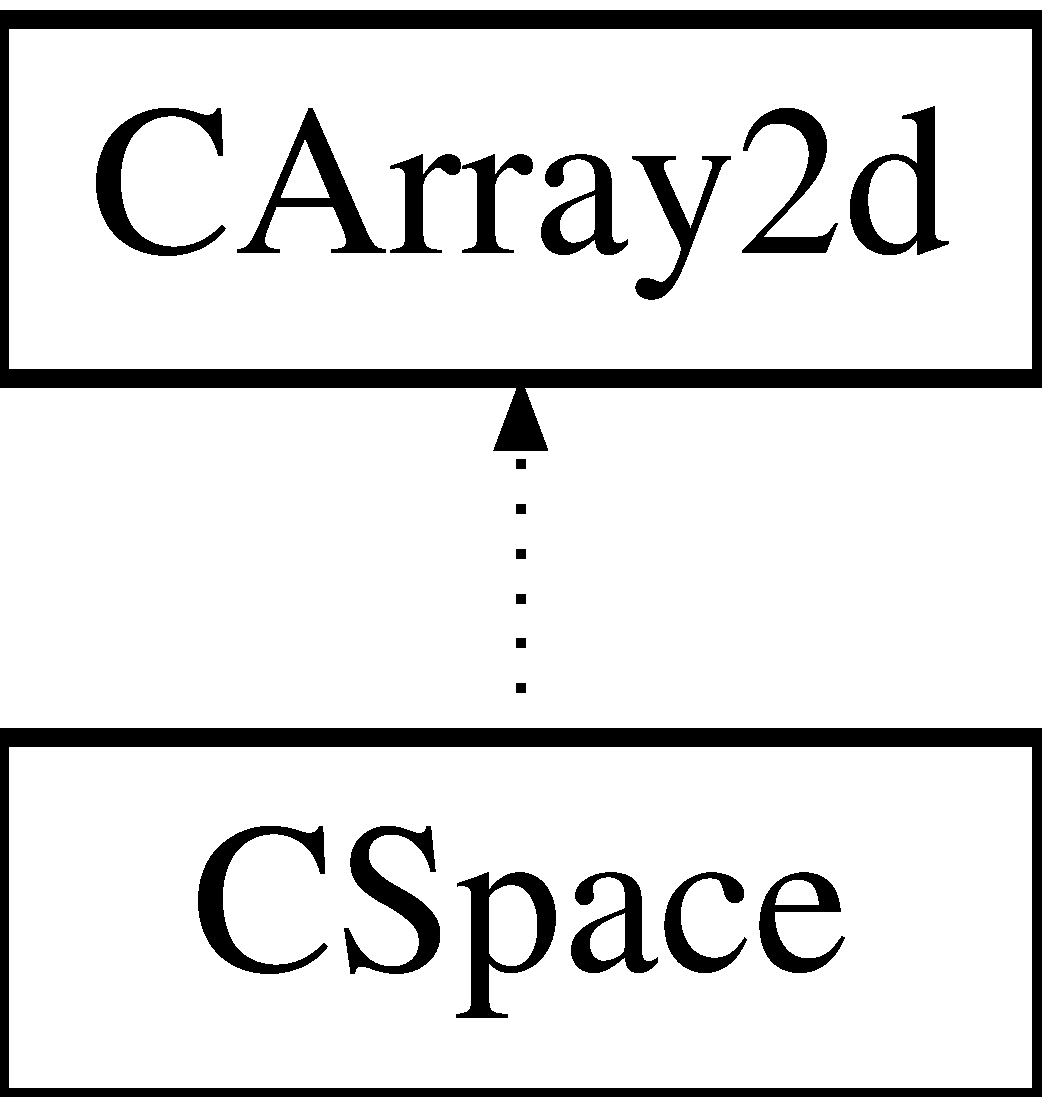
\includegraphics[height=2cm]{classCSpace}
\end{center}
\end{figure}
\subsection*{Public Member Functions}
\begin{DoxyCompactItemize}
\item 
\hyperlink{classCSpace_ab795395372f17e257fa72988e10b206f}{CSpace} (int type=SPACE\_\-TYPE\_\-GRID, int sizeX=SPACE\_\-SIZE\_\-X\_\-DEFAULT, int sizeY=SPACE\_\-SIZE\_\-Y\_\-DEFAULT, BYTE defState=CELL\_\-STATE\_\-EMPTY, \hyperlink{classCConfigCore}{CConfigCore} $\ast$pCC=NULL)
\item 
\hyperlink{classCSpace_a6315ca8443a78458dca1ba8f2b8cf60d}{$\sim$CSpace} ()
\item 
BYTE \hyperlink{classCSpace_a670a753794c1e851cc337f2f312c2538}{at} (int posX, int posY) const 
\item 
BYTE \& \hyperlink{classCSpace_abfac3ba5b7bf020e658b2a52ebcb7f36}{at} (int posX, int posY)
\item 
BYTE \hyperlink{classCSpace_a83689b4589c9f5c8d41931e830d302a1}{atGrid} (int posX, int posY) const 
\item 
BYTE \& \hyperlink{classCSpace_a2ad446a5bb454b65212430b71980a70e}{atGrid} (int posX, int posY)
\item 
BYTE \hyperlink{classCSpace_a7c0381e6e90fc56a8213fba4b047649e}{atTorus} (int posX, int posY) const 
\item 
BYTE \& \hyperlink{classCSpace_a1e2364f59e8dcacd46a5f96d878ca349}{atTorus} (int posX, int posY)
\item 
int \hyperlink{classCSpace_a0358e524cecae683cfbcf526ea99d818}{GetWidth} ()
\item 
int \hyperlink{classCSpace_a00b9bce5ca8303b7bae59e2ab6ce98be}{GetHeight} ()
\item 
int \hyperlink{classCSpace_ae700fc8fa63e62dd559245e832614c65}{GetSpaceType} ()
\item 
int \hyperlink{classCSpace_afe1840ea70f14055a39090ceaec9778e}{GetErrorFlag} ()
\end{DoxyCompactItemize}
\subsection*{Private Attributes}
\begin{DoxyCompactItemize}
\item 
\hypertarget{classCSpace_aedf34dc29d187ea531d730770c74ea5a}{
int \hyperlink{classCSpace_aedf34dc29d187ea531d730770c74ea5a}{iSpaceType}}
\label{classCSpace_aedf34dc29d187ea531d730770c74ea5a}

\begin{DoxyCompactList}\small\item\em space type \item\end{DoxyCompactList}\item 
\hypertarget{classCSpace_a963d2dc89ef63e9a33322561e79a9501}{
BYTE \hyperlink{classCSpace_a963d2dc89ef63e9a33322561e79a9501}{errCell}}
\label{classCSpace_a963d2dc89ef63e9a33322561e79a9501}

\begin{DoxyCompactList}\small\item\em error cell \item\end{DoxyCompactList}\item 
\hypertarget{classCSpace_a4373c80fe05795c2f18d3160d57315a8}{
BYTE \hyperlink{classCSpace_a4373c80fe05795c2f18d3160d57315a8}{byDefCell}}
\label{classCSpace_a4373c80fe05795c2f18d3160d57315a8}

\begin{DoxyCompactList}\small\item\em default value cell \item\end{DoxyCompactList}\end{DoxyCompactItemize}


\subsection{Detailed Description}
inherits \hyperlink{classCArray2d}{CArray2d}, which is carring 2d array, this class implements behaviour of ca space -\/ grid or torus 

\subsection{Constructor \& Destructor Documentation}
\hypertarget{classCSpace_ab795395372f17e257fa72988e10b206f}{
\index{CSpace@{CSpace}!CSpace@{CSpace}}
\index{CSpace@{CSpace}!CSpace@{CSpace}}
\subsubsection[{CSpace}]{\setlength{\rightskip}{0pt plus 5cm}CSpace::CSpace (int {\em type} = {\ttfamily SPACE\_\-TYPE\_\-GRID}, \/  int {\em sizeX} = {\ttfamily SPACE\_\-SIZE\_\-X\_\-DEFAULT}, \/  int {\em sizeY} = {\ttfamily SPACE\_\-SIZE\_\-Y\_\-DEFAULT}, \/  BYTE {\em defState} = {\ttfamily CELL\_\-STATE\_\-EMPTY}, \/  {\bf CConfigCore} $\ast$ {\em pConfigCore} = {\ttfamily NULL})}}
\label{classCSpace_ab795395372f17e257fa72988e10b206f}
class constructor


\begin{DoxyParams}{Parameters}
\item[{\em type}]torus or lattice \item[{\em sizeX}]array width \item[{\em sizeY}]array height \item[{\em defState}]default state \item[{\em $\ast$pConfigCore}]pointer to config class\item[{\em \hyperlink{classCArray2d}{CArray2d}}]\hyperlink{classCSpace}{CSpace} inherits this class \end{DoxyParams}
\hypertarget{classCSpace_a6315ca8443a78458dca1ba8f2b8cf60d}{
\index{CSpace@{CSpace}!$\sim$CSpace@{$\sim$CSpace}}
\index{$\sim$CSpace@{$\sim$CSpace}!CSpace@{CSpace}}
\subsubsection[{$\sim$CSpace}]{\setlength{\rightskip}{0pt plus 5cm}CSpace::$\sim$CSpace ()}}
\label{classCSpace_a6315ca8443a78458dca1ba8f2b8cf60d}
class destructor 

\subsection{Member Function Documentation}
\hypertarget{classCSpace_abfac3ba5b7bf020e658b2a52ebcb7f36}{
\index{CSpace@{CSpace}!at@{at}}
\index{at@{at}!CSpace@{CSpace}}
\subsubsection[{at}]{\setlength{\rightskip}{0pt plus 5cm}BYTE \& CSpace::at (int {\em posX}, \/  int {\em posY})}}
\label{classCSpace_abfac3ba5b7bf020e658b2a52ebcb7f36}
returns reference to element at given coorditates


\begin{DoxyParams}{Parameters}
\item[{\em posX}]position on x-\/axes \item[{\em posY}]position on y-\/axes \end{DoxyParams}
\hypertarget{classCSpace_a670a753794c1e851cc337f2f312c2538}{
\index{CSpace@{CSpace}!at@{at}}
\index{at@{at}!CSpace@{CSpace}}
\subsubsection[{at}]{\setlength{\rightskip}{0pt plus 5cm}BYTE CSpace::at (int {\em posX}, \/  int {\em posY}) const}}
\label{classCSpace_a670a753794c1e851cc337f2f312c2538}
returns element at given coorditates


\begin{DoxyParams}{Parameters}
\item[{\em posX}]position on x-\/axes \item[{\em posY}]position on y-\/axes \end{DoxyParams}
\hypertarget{classCSpace_a2ad446a5bb454b65212430b71980a70e}{
\index{CSpace@{CSpace}!atGrid@{atGrid}}
\index{atGrid@{atGrid}!CSpace@{CSpace}}
\subsubsection[{atGrid}]{\setlength{\rightskip}{0pt plus 5cm}BYTE \& CSpace::atGrid (int {\em posX}, \/  int {\em posY})}}
\label{classCSpace_a2ad446a5bb454b65212430b71980a70e}
returns reference to element at given coorditates with respect to cellular space type \char`\"{}grid\char`\"{}


\begin{DoxyParams}{Parameters}
\item[{\em posX}]position on x-\/axes \item[{\em posY}]position on y-\/axes \end{DoxyParams}
\hypertarget{classCSpace_a83689b4589c9f5c8d41931e830d302a1}{
\index{CSpace@{CSpace}!atGrid@{atGrid}}
\index{atGrid@{atGrid}!CSpace@{CSpace}}
\subsubsection[{atGrid}]{\setlength{\rightskip}{0pt plus 5cm}BYTE CSpace::atGrid (int {\em posX}, \/  int {\em posY}) const}}
\label{classCSpace_a83689b4589c9f5c8d41931e830d302a1}
returns element at given coorditates with respect to cellular space type \char`\"{}grid\char`\"{}


\begin{DoxyParams}{Parameters}
\item[{\em posX}]position on x-\/axes \item[{\em posY}]position on y-\/axes \end{DoxyParams}
\hypertarget{classCSpace_a1e2364f59e8dcacd46a5f96d878ca349}{
\index{CSpace@{CSpace}!atTorus@{atTorus}}
\index{atTorus@{atTorus}!CSpace@{CSpace}}
\subsubsection[{atTorus}]{\setlength{\rightskip}{0pt plus 5cm}BYTE \& CSpace::atTorus (int {\em posX}, \/  int {\em posY})}}
\label{classCSpace_a1e2364f59e8dcacd46a5f96d878ca349}
returns reference to element at given coorditates with respect to cellular space type \char`\"{}torus\char`\"{} -\/ quasi-\/infinate space


\begin{DoxyParams}{Parameters}
\item[{\em posX}]position on x-\/axes \item[{\em posY}]position on y-\/axes \end{DoxyParams}
\hypertarget{classCSpace_a7c0381e6e90fc56a8213fba4b047649e}{
\index{CSpace@{CSpace}!atTorus@{atTorus}}
\index{atTorus@{atTorus}!CSpace@{CSpace}}
\subsubsection[{atTorus}]{\setlength{\rightskip}{0pt plus 5cm}BYTE CSpace::atTorus (int {\em posX}, \/  int {\em posY}) const}}
\label{classCSpace_a7c0381e6e90fc56a8213fba4b047649e}
returns element at given coorditates with respect to cellular space type \char`\"{}torus\char`\"{} -\/ quasi-\/infinate space


\begin{DoxyParams}{Parameters}
\item[{\em posX}]position on x-\/axes \item[{\em posY}]position on y-\/axes \end{DoxyParams}
\hypertarget{classCSpace_afe1840ea70f14055a39090ceaec9778e}{
\index{CSpace@{CSpace}!GetErrorFlag@{GetErrorFlag}}
\index{GetErrorFlag@{GetErrorFlag}!CSpace@{CSpace}}
\subsubsection[{GetErrorFlag}]{\setlength{\rightskip}{0pt plus 5cm}int CSpace::GetErrorFlag ()}}
\label{classCSpace_afe1840ea70f14055a39090ceaec9778e}
return error flag 

Reimplemented from \hyperlink{classCArray2d_afee234adb0190a1d8f3841f75a295e26}{CArray2d}.\hypertarget{classCSpace_a00b9bce5ca8303b7bae59e2ab6ce98be}{
\index{CSpace@{CSpace}!GetHeight@{GetHeight}}
\index{GetHeight@{GetHeight}!CSpace@{CSpace}}
\subsubsection[{GetHeight}]{\setlength{\rightskip}{0pt plus 5cm}int CSpace::GetHeight ()}}
\label{classCSpace_a00b9bce5ca8303b7bae59e2ab6ce98be}
returns array height 

Reimplemented from \hyperlink{classCArray2d_ae019e1beca716a4ea7d368e342fe23a1}{CArray2d}.\hypertarget{classCSpace_ae700fc8fa63e62dd559245e832614c65}{
\index{CSpace@{CSpace}!GetSpaceType@{GetSpaceType}}
\index{GetSpaceType@{GetSpaceType}!CSpace@{CSpace}}
\subsubsection[{GetSpaceType}]{\setlength{\rightskip}{0pt plus 5cm}int CSpace::GetSpaceType ()}}
\label{classCSpace_ae700fc8fa63e62dd559245e832614c65}
returns space type \hypertarget{classCSpace_a0358e524cecae683cfbcf526ea99d818}{
\index{CSpace@{CSpace}!GetWidth@{GetWidth}}
\index{GetWidth@{GetWidth}!CSpace@{CSpace}}
\subsubsection[{GetWidth}]{\setlength{\rightskip}{0pt plus 5cm}int CSpace::GetWidth ()}}
\label{classCSpace_a0358e524cecae683cfbcf526ea99d818}
returns array width 

Reimplemented from \hyperlink{classCArray2d_a7cfeb98b3112d1e147464a7ec2374579}{CArray2d}.

The documentation for this class was generated from the following files:\begin{DoxyCompactItemize}
\item 
Space.h\item 
Space.cpp\end{DoxyCompactItemize}

\hypertarget{classCTFunction}{
\section{CTFunction Class Reference}
\label{classCTFunction}\index{CTFunction@{CTFunction}}
}


{\ttfamily \#include $<$TFunction.h$>$}\subsection*{Public Member Functions}
\begin{DoxyCompactItemize}
\item 
\hyperlink{classCTFunction_a85e48f0a80f493d3e6144f3ed4058ede}{CTFunction} ()
\item 
void \hyperlink{classCTFunction_ae1ba9e9f2baff1687236edc46b23d07f}{SetRulesTable} (\hyperlink{classCRulesTable}{CRulesTable} $\ast$rt)
\item 
void \hyperlink{classCTFunction_ab629990f0e797774b7389e8bd07394a2}{SetConfigCore} (\hyperlink{classCConfigCore}{CConfigCore} $\ast$cc)
\item 
void \hyperlink{classCTFunction_a7d961dbfd8759a0e71180c4112f33ffc}{NextSpace} (\hyperlink{classCSpace}{CSpace} $\ast$sa, \hyperlink{classCSpace}{CSpace} $\ast$sn)
\item 
\hypertarget{classCTFunction_abab8543b07fa119edc0ec039ffb31d83}{
int {\bfseries GetErrorFlag} ()}
\label{classCTFunction_abab8543b07fa119edc0ec039ffb31d83}

\end{DoxyCompactItemize}
\subsection*{Private Member Functions}
\begin{DoxyCompactItemize}
\item 
void \hyperlink{classCTFunction_ac62d3fe86128f015892eccecfef0ddf8}{NextSpaceGenomeStandard} (\hyperlink{classCSpace}{CSpace} $\ast$sa, \hyperlink{classCSpace}{CSpace} $\ast$sn)
\item 
void \hyperlink{classCTFunction_a1e79617602ea9a77be8ee411daa39d6c}{NextSpaceGenomeInstruction} (\hyperlink{classCSpace}{CSpace} $\ast$sa, \hyperlink{classCSpace}{CSpace} $\ast$sn)
\item 
int \hyperlink{classCTFunction_a337b7b2bc4aa55fba6966ed732292836}{CalculateIndexGrid} (\hyperlink{classCSpace}{CSpace} $\ast$s, int x, int y)
\item 
int \hyperlink{classCTFunction_a46be389e8f79729395cb918ab58e63c0}{CalculateIndexTorus} (\hyperlink{classCSpace}{CSpace} $\ast$s, int x, int y)
\end{DoxyCompactItemize}
\subsection*{Private Attributes}
\begin{DoxyCompactItemize}
\item 
\hypertarget{classCTFunction_a72ea1bfa7803e5751d6249bfbf8c7d90}{
\hyperlink{classCRulesTable}{CRulesTable} $\ast$ \hyperlink{classCTFunction_a72ea1bfa7803e5751d6249bfbf8c7d90}{rules}}
\label{classCTFunction_a72ea1bfa7803e5751d6249bfbf8c7d90}

\begin{DoxyCompactList}\small\item\em pointer to rules table \item\end{DoxyCompactList}\item 
\hypertarget{classCTFunction_ae5a61d8280f85a3fa4804b22d6fcdfd0}{
\hyperlink{classCConfigCore}{CConfigCore} $\ast$ \hyperlink{classCTFunction_ae5a61d8280f85a3fa4804b22d6fcdfd0}{pConfigCore}}
\label{classCTFunction_ae5a61d8280f85a3fa4804b22d6fcdfd0}

\begin{DoxyCompactList}\small\item\em pointer to config class \item\end{DoxyCompactList}\item 
\hypertarget{classCTFunction_a84a79b8b4aa3d09537e5900de355e63d}{
int \hyperlink{classCTFunction_a84a79b8b4aa3d09537e5900de355e63d}{iErrFlag}}
\label{classCTFunction_a84a79b8b4aa3d09537e5900de355e63d}

\begin{DoxyCompactList}\small\item\em error flag \item\end{DoxyCompactList}\end{DoxyCompactItemize}


\subsection{Detailed Description}
transition function performs all calculations of CA for all cell in space it calculates index to genome, gets gene using \hyperlink{classCRulesTable}{CRulesTable} class and writes new value of cell into next-\/gen space 

\subsection{Constructor \& Destructor Documentation}
\hypertarget{classCTFunction_a85e48f0a80f493d3e6144f3ed4058ede}{
\index{CTFunction@{CTFunction}!CTFunction@{CTFunction}}
\index{CTFunction@{CTFunction}!CTFunction@{CTFunction}}
\subsubsection[{CTFunction}]{\setlength{\rightskip}{0pt plus 5cm}CTFunction::CTFunction ()}}
\label{classCTFunction_a85e48f0a80f493d3e6144f3ed4058ede}
class constructor 

\subsection{Member Function Documentation}
\hypertarget{classCTFunction_a337b7b2bc4aa55fba6966ed732292836}{
\index{CTFunction@{CTFunction}!CalculateIndexGrid@{CalculateIndexGrid}}
\index{CalculateIndexGrid@{CalculateIndexGrid}!CTFunction@{CTFunction}}
\subsubsection[{CalculateIndexGrid}]{\setlength{\rightskip}{0pt plus 5cm}int CTFunction::CalculateIndexGrid ({\bf CSpace} $\ast$ {\em s}, \/  int {\em x}, \/  int {\em y})\hspace{0.3cm}{\ttfamily  \mbox{[}private\mbox{]}}}}
\label{classCTFunction_a337b7b2bc4aa55fba6966ed732292836}
calculates index into genome using \char`\"{}grid\char`\"{} rules


\begin{DoxyParams}{Parameters}
\item[{\em $\ast$s}]pointer to actual ca space \item[{\em x}]x coordinate of actual cell \item[{\em y}]y coordinate of actual cell \end{DoxyParams}
\hypertarget{classCTFunction_a46be389e8f79729395cb918ab58e63c0}{
\index{CTFunction@{CTFunction}!CalculateIndexTorus@{CalculateIndexTorus}}
\index{CalculateIndexTorus@{CalculateIndexTorus}!CTFunction@{CTFunction}}
\subsubsection[{CalculateIndexTorus}]{\setlength{\rightskip}{0pt plus 5cm}int CTFunction::CalculateIndexTorus ({\bf CSpace} $\ast$ {\em s}, \/  int {\em x}, \/  int {\em y})\hspace{0.3cm}{\ttfamily  \mbox{[}private\mbox{]}}}}
\label{classCTFunction_a46be389e8f79729395cb918ab58e63c0}
calculates index into genome using \char`\"{}torus\char`\"{} rules


\begin{DoxyParams}{Parameters}
\item[{\em $\ast$s}]pointer to actual ca space \item[{\em x}]x coordinate of actual cell \item[{\em y}]y coordinate of actual cell \end{DoxyParams}
\hypertarget{classCTFunction_a7d961dbfd8759a0e71180c4112f33ffc}{
\index{CTFunction@{CTFunction}!NextSpace@{NextSpace}}
\index{NextSpace@{NextSpace}!CTFunction@{CTFunction}}
\subsubsection[{NextSpace}]{\setlength{\rightskip}{0pt plus 5cm}void CTFunction::NextSpace ({\bf CSpace} $\ast$ {\em sa}, \/  {\bf CSpace} $\ast$ {\em sn})}}
\label{classCTFunction_a7d961dbfd8759a0e71180c4112f33ffc}
computes new ca array from old one with rules table given


\begin{DoxyParams}{Parameters}
\item[{\em $\ast$sa}]ca space actual \item[{\em $\ast$sn}]ca space next \end{DoxyParams}
\hypertarget{classCTFunction_a1e79617602ea9a77be8ee411daa39d6c}{
\index{CTFunction@{CTFunction}!NextSpaceGenomeInstruction@{NextSpaceGenomeInstruction}}
\index{NextSpaceGenomeInstruction@{NextSpaceGenomeInstruction}!CTFunction@{CTFunction}}
\subsubsection[{NextSpaceGenomeInstruction}]{\setlength{\rightskip}{0pt plus 5cm}void CTFunction::NextSpaceGenomeInstruction ({\bf CSpace} $\ast$ {\em sa}, \/  {\bf CSpace} $\ast$ {\em sn})\hspace{0.3cm}{\ttfamily  \mbox{[}private\mbox{]}}}}
\label{classCTFunction_a1e79617602ea9a77be8ee411daa39d6c}
computes new ca space with instruction genome, NOT IMPLEMENTED


\begin{DoxyParams}{Parameters}
\item[{\em $\ast$sa}]ca space actual \item[{\em $\ast$sn}]ca space next \end{DoxyParams}
\hypertarget{classCTFunction_ac62d3fe86128f015892eccecfef0ddf8}{
\index{CTFunction@{CTFunction}!NextSpaceGenomeStandard@{NextSpaceGenomeStandard}}
\index{NextSpaceGenomeStandard@{NextSpaceGenomeStandard}!CTFunction@{CTFunction}}
\subsubsection[{NextSpaceGenomeStandard}]{\setlength{\rightskip}{0pt plus 5cm}void CTFunction::NextSpaceGenomeStandard ({\bf CSpace} $\ast$ {\em sa}, \/  {\bf CSpace} $\ast$ {\em sn})\hspace{0.3cm}{\ttfamily  \mbox{[}private\mbox{]}}}}
\label{classCTFunction_ac62d3fe86128f015892eccecfef0ddf8}
computes new ca space with standard, non-\/instruction genome


\begin{DoxyParams}{Parameters}
\item[{\em $\ast$sa}]ca space actual \item[{\em $\ast$sn}]ca space next \end{DoxyParams}
\hypertarget{classCTFunction_ab629990f0e797774b7389e8bd07394a2}{
\index{CTFunction@{CTFunction}!SetConfigCore@{SetConfigCore}}
\index{SetConfigCore@{SetConfigCore}!CTFunction@{CTFunction}}
\subsubsection[{SetConfigCore}]{\setlength{\rightskip}{0pt plus 5cm}void CTFunction::SetConfigCore ({\bf CConfigCore} $\ast$ {\em cc})}}
\label{classCTFunction_ab629990f0e797774b7389e8bd07394a2}
sets config class \hypertarget{classCTFunction_ae1ba9e9f2baff1687236edc46b23d07f}{
\index{CTFunction@{CTFunction}!SetRulesTable@{SetRulesTable}}
\index{SetRulesTable@{SetRulesTable}!CTFunction@{CTFunction}}
\subsubsection[{SetRulesTable}]{\setlength{\rightskip}{0pt plus 5cm}void CTFunction::SetRulesTable ({\bf CRulesTable} $\ast$ {\em rt})}}
\label{classCTFunction_ae1ba9e9f2baff1687236edc46b23d07f}
sets actual rules table, which mapping genome from ga


\begin{DoxyParams}{Parameters}
\item[{\em $\ast$rt}]pointer to rules table class \end{DoxyParams}


The documentation for this class was generated from the following files:\begin{DoxyCompactItemize}
\item 
TFunction.h\item 
TFunction.cpp\end{DoxyCompactItemize}

\hypertarget{classCThreadCore}{
\section{CThreadCore Class Reference}
\label{classCThreadCore}\index{CThreadCore@{CThreadCore}}
}


{\ttfamily \#include $<$ThreadCore.h$>$}\subsection*{Signals}
\begin{DoxyCompactItemize}
\item 
\hypertarget{classCThreadCore_a715eb432de93b30314f523e58bb6381b}{
void {\bfseries SignalErrCore} (int)}
\label{classCThreadCore_a715eb432de93b30314f523e58bb6381b}

\item 
\hypertarget{classCThreadCore_a8dfdedd72e8e108b4c72bc26cf881149}{
void {\bfseries SignalInitCoreDone} ()}
\label{classCThreadCore_a8dfdedd72e8e108b4c72bc26cf881149}

\item 
\hypertarget{classCThreadCore_a233ff4a618739e9c096fc3eeed4b4296}{
void {\bfseries SignalNewDataAvailable} ()}
\label{classCThreadCore_a233ff4a618739e9c096fc3eeed4b4296}

\item 
\hypertarget{classCThreadCore_ad418dc626ec7ac1c3f7b198d200b694d}{
void {\bfseries SignalThreadState} (int)}
\label{classCThreadCore_ad418dc626ec7ac1c3f7b198d200b694d}

\end{DoxyCompactItemize}
\subsection*{Public Member Functions}
\begin{DoxyCompactItemize}
\item 
\hyperlink{classCThreadCore_a3bf4b7a3b3dab03741d538e35dcfb9dc}{CThreadCore} ()
\item 
\hyperlink{classCThreadCore_a059d1d66522f2e611d83abafda575564}{$\sim$CThreadCore} ()
\item 
void \hyperlink{classCThreadCore_af78150953eef0f33cf28125f137d7fbb}{run} ()
\item 
void \hyperlink{classCThreadCore_adfbf9fecc93acfb6f000f4d936a0f136}{SetConfigCore} (\hyperlink{classCConfigCore}{CConfigCore} $\ast$cc)
\item 
void \hyperlink{classCThreadCore_aebf817096243757f85c09221b9271c8d}{SetCoreSpace} (\hyperlink{classCSpace}{CSpace} $\ast$cs)
\item 
void \hyperlink{classCThreadCore_a21b99b77c6e6f2ba8c3616c82185d6ef}{SetCoreDataGA} (struct \hyperlink{structstThreadCoreDataGA}{stThreadCoreDataGA} $\ast$tcdga)
\item 
void \hyperlink{classCThreadCore_ada7f488e5307d5996cea904f5fa9d62b}{SetMutex} (QMutex $\ast$mc)
\item 
void \hyperlink{classCThreadCore_a68d67f8c9b9cb9592c014f3c8c27c5d7}{SetWaitCondition} (QWaitCondition $\ast$wcc)
\item 
void \hyperlink{classCThreadCore_a12e9d20ea581f945c72e6648a313e3b3}{SetCoreDataExpiration} (bool $\ast$be)
\item 
void \hyperlink{classCThreadCore_a001ae8aefae184bcb4274793a7633df6}{SetSimulationRunning} (bool $\ast$sr)
\item 
\hyperlink{classCSpace}{CSpace} $\ast$ \hyperlink{classCThreadCore_ae65e6c5c661c97f58d795907da19377a}{GetSpace} ()
\item 
\hyperlink{classCSpace}{CSpace} $\ast$ \hyperlink{classCThreadCore_aab198fc60402f7c65e5085404d9b75ae}{GetInitSpace} ()
\item 
bool \hyperlink{classCThreadCore_a85b03fa847d72661b2710af2beaa70dd}{IsInitDone} ()
\item 
void \hyperlink{classCThreadCore_a656208f8a0c3915d6786e317ba59184f}{TerminateThreadLoop} ()
\item 
bool \hyperlink{classCThreadCore_a817d1a465e68edcb480a30d66ec7f5c2}{CheckThreadLoopTermination} ()
\item 
void \hyperlink{classCThreadCore_ad44d9a6277ac3c02715b35eb44110c07}{TerminateCaRun} ()
\item 
bool \hyperlink{classCThreadCore_ac19af4cab9673daf796044312634c97a}{CheckCaRunTermination} ()
\item 
int \hyperlink{classCThreadCore_a584f4b6a6afec6903ca7cb5f9eac96b2}{GetErrorFlag} ()
\end{DoxyCompactItemize}
\subsection*{Private Member Functions}
\begin{DoxyCompactItemize}
\item 
void \hyperlink{classCThreadCore_a585fd3734edc146086bc42187fd56bc6}{InitCore} ()
\item 
void \hyperlink{classCThreadCore_a6d63012cb404af5d7b18017d8299a603}{ReinitCore} ()
\item 
void \hyperlink{classCThreadCore_ad0bfe748e42ad65bbe82df1070c8c95e}{InitCoreGeneticAlgorithm} ()
\item 
void \hyperlink{classCThreadCore_a1dc7525d74dba3c1fa0a94057596c0a2}{InitCoreCellularAutomata} ()
\item 
void \hyperlink{classCThreadCore_a6cc4724d18c05cd2d06833c986cc569d}{InitCoreCAMemory} ()
\item 
void \hyperlink{classCThreadCore_abde63c16350bd57c9ecc539195a84e91}{InitExport} ()
\item 
void \hyperlink{classCThreadCore_a4e710409fd00cd204c837db052506879}{InitTmpCAs} ()
\item 
void \hyperlink{classCThreadCore_a6a70230547c401faba79d362df341bae}{ClearTmpCAs} ()
\item 
bool \hyperlink{classCThreadCore_a27d1fd877a64e906a250898a36aeb730}{CheckCorePointers} ()
\item 
void \hyperlink{classCThreadCore_af979f38a80787229941f03512e003c09}{WriteCASpaceFromCoreIntoCA} ()
\item 
void \hyperlink{classCThreadCore_a427dd34ccf958e15f9b9754ca4b21088}{WriteDataCAToCore} ()
\item 
void \hyperlink{classCThreadCore_a533ca5b498cbe0395dedd01e1646c973}{WriteDataGAToCore} ()
\item 
void \hyperlink{classCThreadCore_a4fff3c00394bcaffae4875a7fb28a335}{SyncDataWithCore} ()
\item 
void \hyperlink{classCThreadCore_a780fc802d644b0e4d992558df2f27c5d}{SetCoreDataValidity} (bool dve)
\item 
void \hyperlink{classCThreadCore_a597d1ee93090b677f89f3ac6005e8561}{RunGuiMode} (int call\_\-pos)
\item 
void \hyperlink{classCThreadCore_ad76c05c9748da357d926c66a52fecfdc}{FileExportGa} (int call\_\-pos)
\item 
void \hyperlink{classCThreadCore_a8a25b573f3189377f4f34b75a65dd063}{FileExportCaInit} ()
\item 
void \hyperlink{classCThreadCore_a25cbacbf0e0c79aab05aee3a41a1043f}{FileExportCaSteps} (\hyperlink{classCGenome}{CGenome} $\ast$gen)
\item 
void \hyperlink{classCThreadCore_a73af8250e870e24d41f99f7e576fb466}{RunGenomeCaSimulation} (\hyperlink{classCGenome}{CGenome} $\ast$gen)
\item 
void \hyperlink{classCThreadCore_aecc92d11204f96cd0c658cdc3b925f58}{StoreGenomeDataForGui} (int mode)
\end{DoxyCompactItemize}
\subsection*{Private Attributes}
\begin{DoxyCompactItemize}
\item 
\hypertarget{classCThreadCore_a5227042e1033fe13a8008f5e168be186}{
bool \hyperlink{classCThreadCore_a5227042e1033fe13a8008f5e168be186}{bInitDone}}
\label{classCThreadCore_a5227042e1033fe13a8008f5e168be186}

\begin{DoxyCompactList}\small\item\em init done var \item\end{DoxyCompactList}\item 
\hypertarget{classCThreadCore_a600744bc7de7dc91afe82eb8e1f1c339}{
bool \hyperlink{classCThreadCore_a600744bc7de7dc91afe82eb8e1f1c339}{bEvoExit}}
\label{classCThreadCore_a600744bc7de7dc91afe82eb8e1f1c339}

\begin{DoxyCompactList}\small\item\em evolution (thread) termination var \item\end{DoxyCompactList}\item 
\hypertarget{classCThreadCore_a7583f058641e2ddd3f7ff6f74a49a3e5}{
bool \hyperlink{classCThreadCore_a7583f058641e2ddd3f7ff6f74a49a3e5}{bCaRunTermination}}
\label{classCThreadCore_a7583f058641e2ddd3f7ff6f74a49a3e5}

\begin{DoxyCompactList}\small\item\em ca simulator terminated var \item\end{DoxyCompactList}\item 
\hypertarget{classCThreadCore_afba26cc1a0606dbc2a61bc5cc1b606f9}{
\hyperlink{classCGeneticAlgorithm}{CGeneticAlgorithm} $\ast$ \hyperlink{classCThreadCore_afba26cc1a0606dbc2a61bc5cc1b606f9}{ga}}
\label{classCThreadCore_afba26cc1a0606dbc2a61bc5cc1b606f9}

\begin{DoxyCompactList}\small\item\em pointer to instance of main GA class \item\end{DoxyCompactList}\item 
\hypertarget{classCThreadCore_a66fd0ab7d1c294b88d6354073a0aaeb1}{
\hyperlink{classCCellularAutomata}{CCellularAutomata} $\ast$ \hyperlink{classCThreadCore_a66fd0ab7d1c294b88d6354073a0aaeb1}{ca}}
\label{classCThreadCore_a66fd0ab7d1c294b88d6354073a0aaeb1}

\begin{DoxyCompactList}\small\item\em pointer to instance of main CA class \item\end{DoxyCompactList}\item 
\hypertarget{classCThreadCore_a8080361bc3a14e997aa26f8da2b6144a}{
\hyperlink{classCConfigCore}{CConfigCore} $\ast$ \hyperlink{classCThreadCore_a8080361bc3a14e997aa26f8da2b6144a}{pConfigCore}}
\label{classCThreadCore_a8080361bc3a14e997aa26f8da2b6144a}

\begin{DoxyCompactList}\small\item\em pointer to config class \item\end{DoxyCompactList}\item 
\hypertarget{classCThreadCore_aa6919fadf11ae4ae63f1c9d23d10f7bd}{
\hyperlink{classCSpace}{CSpace} $\ast$ \hyperlink{classCThreadCore_aa6919fadf11ae4ae63f1c9d23d10f7bd}{pCoreSpace}}
\label{classCThreadCore_aa6919fadf11ae4ae63f1c9d23d10f7bd}

\begin{DoxyCompactList}\small\item\em pointer to \hyperlink{classCCore}{CCore} ca space used for sending data into gui \item\end{DoxyCompactList}\item 
\hypertarget{classCThreadCore_a1fc888c8bd4964441440a0bca709975e}{
\hyperlink{classCExportGA}{CExportGA} \hyperlink{classCThreadCore_a1fc888c8bd4964441440a0bca709975e}{exportGa}}
\label{classCThreadCore_a1fc888c8bd4964441440a0bca709975e}

\begin{DoxyCompactList}\small\item\em instance of export ga class \item\end{DoxyCompactList}\item 
\hypertarget{classCThreadCore_a08a252657f47ad43a53af77d19969150}{
\hyperlink{classCExportCA}{CExportCA} \hyperlink{classCThreadCore_a08a252657f47ad43a53af77d19969150}{exportCa}}
\label{classCThreadCore_a08a252657f47ad43a53af77d19969150}

\begin{DoxyCompactList}\small\item\em instance of export ca class \item\end{DoxyCompactList}\item 
\hypertarget{classCThreadCore_a0611597f1c547b6ed601f7aec10446f6}{
\hyperlink{classCImportGA}{CImportGA} \hyperlink{classCThreadCore_a0611597f1c547b6ed601f7aec10446f6}{importGa}}
\label{classCThreadCore_a0611597f1c547b6ed601f7aec10446f6}

\begin{DoxyCompactList}\small\item\em instance of import genome class \item\end{DoxyCompactList}\item 
\hypertarget{classCThreadCore_ac4d055b467336ef1f9195e44e3712bc3}{
\hyperlink{classCExportLog}{CExportLog} \hyperlink{classCThreadCore_ac4d055b467336ef1f9195e44e3712bc3}{exportLog}}
\label{classCThreadCore_ac4d055b467336ef1f9195e44e3712bc3}

\begin{DoxyCompactList}\small\item\em instance of export error log class \item\end{DoxyCompactList}\item 
\hypertarget{classCThreadCore_a8572b9b637d9202ccc81bbc0199091f7}{
\hyperlink{classCGenome}{CGenome} $\ast$ \hyperlink{classCThreadCore_a8572b9b637d9202ccc81bbc0199091f7}{bestGenome}}
\label{classCThreadCore_a8572b9b637d9202ccc81bbc0199091f7}

\begin{DoxyCompactList}\small\item\em best genome in actual evolution run \item\end{DoxyCompactList}\item 
\hypertarget{classCThreadCore_ae7f25c80e6a63af6cfe99cf835bda7dd}{
\hyperlink{classCGenome}{CGenome} $\ast$ \hyperlink{classCThreadCore_ae7f25c80e6a63af6cfe99cf835bda7dd}{bestGenomeTotal}}
\label{classCThreadCore_ae7f25c80e6a63af6cfe99cf835bda7dd}

\begin{DoxyCompactList}\small\item\em pointer to total best genome class (best genome of all independet evolution runs) \item\end{DoxyCompactList}\item 
\hypertarget{classCThreadCore_abc716aac8fde953bdffb62a2c0cd7406}{
\hyperlink{classCGenome}{CGenome} $\ast$ \hyperlink{classCThreadCore_abc716aac8fde953bdffb62a2c0cd7406}{actGenome}}
\label{classCThreadCore_abc716aac8fde953bdffb62a2c0cd7406}

\begin{DoxyCompactList}\small\item\em pointer to actual genome class \item\end{DoxyCompactList}\item 
\hypertarget{classCThreadCore_ab5bfacc207f66af97ba53cf31249b33b}{
\hyperlink{classCGenome}{CGenome} $\ast$ \hyperlink{classCThreadCore_ab5bfacc207f66af97ba53cf31249b33b}{importGenome}}
\label{classCThreadCore_ab5bfacc207f66af97ba53cf31249b33b}

\begin{DoxyCompactList}\small\item\em pointer to import genome class \item\end{DoxyCompactList}\item 
\hypertarget{classCThreadCore_a6b038d21e01e0ccfa5fe741cb42cd29b}{
QMutex $\ast$ \hyperlink{classCThreadCore_a6b038d21e01e0ccfa5fe741cb42cd29b}{pMutexCore}}
\label{classCThreadCore_a6b038d21e01e0ccfa5fe741cb42cd29b}

\begin{DoxyCompactList}\small\item\em pointer to \hyperlink{classCCore}{CCore} var used for threads sync \item\end{DoxyCompactList}\item 
\hypertarget{classCThreadCore_a8bd4c7324c6d5daa73b1d7a8b3c7799a}{
QWaitCondition $\ast$ \hyperlink{classCThreadCore_a8bd4c7324c6d5daa73b1d7a8b3c7799a}{pWaitCCore}}
\label{classCThreadCore_a8bd4c7324c6d5daa73b1d7a8b3c7799a}

\begin{DoxyCompactList}\small\item\em pointer to \hyperlink{classCCore}{CCore} var used for threads sync \item\end{DoxyCompactList}\item 
\hypertarget{classCThreadCore_aaaa0f369415f94bafde05c09ee4467c6}{
bool $\ast$ \hyperlink{classCThreadCore_aaaa0f369415f94bafde05c09ee4467c6}{bCoreDataExpired}}
\label{classCThreadCore_aaaa0f369415f94bafde05c09ee4467c6}

\begin{DoxyCompactList}\small\item\em pointer to \hyperlink{classCCore}{CCore} var defining if data send into \hyperlink{classCCore}{CCore} are displayed in gui \item\end{DoxyCompactList}\item 
\hypertarget{classCThreadCore_aec58c27de7ab78615bb759ecb5c5d5dd}{
bool $\ast$ \hyperlink{classCThreadCore_aec58c27de7ab78615bb759ecb5c5d5dd}{bCoreSimRunning}}
\label{classCThreadCore_aec58c27de7ab78615bb759ecb5c5d5dd}

\begin{DoxyCompactList}\small\item\em pointer to \hyperlink{classCCore}{CCore} var defining if this thread should start compute \item\end{DoxyCompactList}\item 
\hypertarget{classCThreadCore_a806a6c3785b9729b6f8013aab99fd0df}{
std::string \hyperlink{classCThreadCore_a806a6c3785b9729b6f8013aab99fd0df}{gol}}
\label{classCThreadCore_a806a6c3785b9729b6f8013aab99fd0df}

\begin{DoxyCompactList}\small\item\em i am not sure .. probably from very early version for GoL genome \item\end{DoxyCompactList}\item 
\hypertarget{classCThreadCore_a1104adbe15044f2acc27d3a433242fa0}{
int \hyperlink{classCThreadCore_a1104adbe15044f2acc27d3a433242fa0}{iErrFlag}}
\label{classCThreadCore_a1104adbe15044f2acc27d3a433242fa0}

\begin{DoxyCompactList}\small\item\em error flag \item\end{DoxyCompactList}\item 
\hypertarget{classCThreadCore_a68a415431dad357abc1f4d2f09fd7758}{
struct \hyperlink{structstThreadCoreDataGA}{stThreadCoreDataGA} \hyperlink{classCThreadCore_a68a415431dad357abc1f4d2f09fd7758}{dataGaAct}}
\label{classCThreadCore_a68a415431dad357abc1f4d2f09fd7758}

\begin{DoxyCompactList}\small\item\em actually used genome \item\end{DoxyCompactList}\item 
\hypertarget{classCThreadCore_ae4a6c06b235fd91b91e54a1700f72607}{
struct \hyperlink{structstThreadCoreDataGA}{stThreadCoreDataGA} \hyperlink{classCThreadCore_ae4a6c06b235fd91b91e54a1700f72607}{dataGaMax}}
\label{classCThreadCore_ae4a6c06b235fd91b91e54a1700f72607}

\begin{DoxyCompactList}\small\item\em best genome of this run \item\end{DoxyCompactList}\item 
\hypertarget{classCThreadCore_abd1b12027b0f0472b446de0d87b8081f}{
struct \hyperlink{structstThreadCoreDataGA}{stThreadCoreDataGA} \hyperlink{classCThreadCore_abd1b12027b0f0472b446de0d87b8081f}{dataGaTot}}
\label{classCThreadCore_abd1b12027b0f0472b446de0d87b8081f}

\begin{DoxyCompactList}\small\item\em ga data of total best genome (best genome of all independent runs) \item\end{DoxyCompactList}\item 
\hypertarget{classCThreadCore_a6e090ebaca99c35e652d47f9fbaabe93}{
struct \hyperlink{structstThreadCoreDataGA}{stThreadCoreDataGA} $\ast$ \hyperlink{classCThreadCore_a6e090ebaca99c35e652d47f9fbaabe93}{dataGaToGui}}
\label{classCThreadCore_a6e090ebaca99c35e652d47f9fbaabe93}

\begin{DoxyCompactList}\small\item\em pointer to data struct from which data to gui will be send \item\end{DoxyCompactList}\item 
\hypertarget{classCThreadCore_abf3c30352d0c198c224177d6638f3d95}{
struct \hyperlink{structstThreadCoreDataGA}{stThreadCoreDataGA} $\ast$ \hyperlink{classCThreadCore_abf3c30352d0c198c224177d6638f3d95}{pCoreDataGa}}
\label{classCThreadCore_abf3c30352d0c198c224177d6638f3d95}

\begin{DoxyCompactList}\small\item\em pointer to \hyperlink{classCCore}{CCore} ga data struct \item\end{DoxyCompactList}\item 
\hypertarget{classCThreadCore_a5139054ea143d81458c0c5827623495b}{
QString \hyperlink{classCThreadCore_a5139054ea143d81458c0c5827623495b}{exportFileGa}}
\label{classCThreadCore_a5139054ea143d81458c0c5827623495b}

\begin{DoxyCompactList}\small\item\em name of ga export file \item\end{DoxyCompactList}\item 
\hypertarget{classCThreadCore_ad814a51d840bd6cad637664c2e9a9bd9}{
QString \hyperlink{classCThreadCore_ad814a51d840bd6cad637664c2e9a9bd9}{exportFileCa}}
\label{classCThreadCore_ad814a51d840bd6cad637664c2e9a9bd9}

\begin{DoxyCompactList}\small\item\em name of ca export file \item\end{DoxyCompactList}\item 
\hypertarget{classCThreadCore_a955bf734623372149659859157b456bf}{
\hyperlink{classCCellularAutomata}{CCellularAutomata} $\ast$ \hyperlink{classCThreadCore_a955bf734623372149659859157b456bf}{tmpVecCA}}
\label{classCThreadCore_a955bf734623372149659859157b456bf}

\begin{DoxyCompactList}\small\item\em pointer to CA class \item\end{DoxyCompactList}\item 
\hypertarget{classCThreadCore_aef7310c60e87ac0ee0a45e5b9220d14b}{
std::vector$<$ \hyperlink{classCCellularAutomata}{CCellularAutomata} $\ast$ $>$ \hyperlink{classCThreadCore_aef7310c60e87ac0ee0a45e5b9220d14b}{vecTmpCAs}}
\label{classCThreadCore_aef7310c60e87ac0ee0a45e5b9220d14b}

\begin{DoxyCompactList}\small\item\em vector with cellular automatons \item\end{DoxyCompactList}\item 
\hypertarget{classCThreadCore_a97c80e8cf2c9e0461636a309d596438a}{
\hyperlink{classCConfigCore}{CConfigCore} \hyperlink{classCThreadCore_a97c80e8cf2c9e0461636a309d596438a}{configTmpCAs}}
\label{classCThreadCore_a97c80e8cf2c9e0461636a309d596438a}

\begin{DoxyCompactList}\small\item\em config core for tmp CAs \item\end{DoxyCompactList}\end{DoxyCompactItemize}


\subsection{Detailed Description}
main compute class of evolution this class is using classes of GA and CA 

\subsection{Constructor \& Destructor Documentation}
\hypertarget{classCThreadCore_a3bf4b7a3b3dab03741d538e35dcfb9dc}{
\index{CThreadCore@{CThreadCore}!CThreadCore@{CThreadCore}}
\index{CThreadCore@{CThreadCore}!CThreadCore@{CThreadCore}}
\subsubsection[{CThreadCore}]{\setlength{\rightskip}{0pt plus 5cm}CThreadCore::CThreadCore ()}}
\label{classCThreadCore_a3bf4b7a3b3dab03741d538e35dcfb9dc}
class constructor \hypertarget{classCThreadCore_a059d1d66522f2e611d83abafda575564}{
\index{CThreadCore@{CThreadCore}!$\sim$CThreadCore@{$\sim$CThreadCore}}
\index{$\sim$CThreadCore@{$\sim$CThreadCore}!CThreadCore@{CThreadCore}}
\subsubsection[{$\sim$CThreadCore}]{\setlength{\rightskip}{0pt plus 5cm}CThreadCore::$\sim$CThreadCore ()}}
\label{classCThreadCore_a059d1d66522f2e611d83abafda575564}
class destructor 

\subsection{Member Function Documentation}
\hypertarget{classCThreadCore_ac19af4cab9673daf796044312634c97a}{
\index{CThreadCore@{CThreadCore}!CheckCaRunTermination@{CheckCaRunTermination}}
\index{CheckCaRunTermination@{CheckCaRunTermination}!CThreadCore@{CThreadCore}}
\subsubsection[{CheckCaRunTermination}]{\setlength{\rightskip}{0pt plus 5cm}bool CThreadCore::CheckCaRunTermination ()}}
\label{classCThreadCore_ac19af4cab9673daf796044312634c97a}
checks, if ca simulator was abord from gui \hypertarget{classCThreadCore_a27d1fd877a64e906a250898a36aeb730}{
\index{CThreadCore@{CThreadCore}!CheckCorePointers@{CheckCorePointers}}
\index{CheckCorePointers@{CheckCorePointers}!CThreadCore@{CThreadCore}}
\subsubsection[{CheckCorePointers}]{\setlength{\rightskip}{0pt plus 5cm}bool CThreadCore::CheckCorePointers ()\hspace{0.3cm}{\ttfamily  \mbox{[}private\mbox{]}}}}
\label{classCThreadCore_a27d1fd877a64e906a250898a36aeb730}
checks if all pointers to \hyperlink{classCCore}{CCore} var are correctly set \hypertarget{classCThreadCore_a817d1a465e68edcb480a30d66ec7f5c2}{
\index{CThreadCore@{CThreadCore}!CheckThreadLoopTermination@{CheckThreadLoopTermination}}
\index{CheckThreadLoopTermination@{CheckThreadLoopTermination}!CThreadCore@{CThreadCore}}
\subsubsection[{CheckThreadLoopTermination}]{\setlength{\rightskip}{0pt plus 5cm}bool CThreadCore::CheckThreadLoopTermination ()}}
\label{classCThreadCore_a817d1a465e68edcb480a30d66ec7f5c2}
checks if app/thread core was terminated \hypertarget{classCThreadCore_a6a70230547c401faba79d362df341bae}{
\index{CThreadCore@{CThreadCore}!ClearTmpCAs@{ClearTmpCAs}}
\index{ClearTmpCAs@{ClearTmpCAs}!CThreadCore@{CThreadCore}}
\subsubsection[{ClearTmpCAs}]{\setlength{\rightskip}{0pt plus 5cm}void CThreadCore::ClearTmpCAs ()\hspace{0.3cm}{\ttfamily  \mbox{[}private\mbox{]}}}}
\label{classCThreadCore_a6a70230547c401faba79d362df341bae}
clears tmp CAs which are used for evolving vseo chromosomes \hypertarget{classCThreadCore_a8a25b573f3189377f4f34b75a65dd063}{
\index{CThreadCore@{CThreadCore}!FileExportCaInit@{FileExportCaInit}}
\index{FileExportCaInit@{FileExportCaInit}!CThreadCore@{CThreadCore}}
\subsubsection[{FileExportCaInit}]{\setlength{\rightskip}{0pt plus 5cm}void CThreadCore::FileExportCaInit ()\hspace{0.3cm}{\ttfamily  \mbox{[}private\mbox{]}}}}
\label{classCThreadCore_a8a25b573f3189377f4f34b75a65dd063}
exports init ca configuration into png (using \hyperlink{classCExportCA}{CExportCA} class) \hypertarget{classCThreadCore_a25cbacbf0e0c79aab05aee3a41a1043f}{
\index{CThreadCore@{CThreadCore}!FileExportCaSteps@{FileExportCaSteps}}
\index{FileExportCaSteps@{FileExportCaSteps}!CThreadCore@{CThreadCore}}
\subsubsection[{FileExportCaSteps}]{\setlength{\rightskip}{0pt plus 5cm}void CThreadCore::FileExportCaSteps ({\bf CGenome} $\ast$ {\em gen})\hspace{0.3cm}{\ttfamily  \mbox{[}private\mbox{]}}}}
\label{classCThreadCore_a25cbacbf0e0c79aab05aee3a41a1043f}
exports all steps (from period) of ca run of object with selected genome for export space into png is used \hyperlink{classCExportCA}{CExportCA} class example: exports 4 png-\/s of glider with game of life rules


\begin{DoxyParams}{Parameters}
\item[{\em $\ast$gen}]pointer to genome \end{DoxyParams}
\hypertarget{classCThreadCore_ad76c05c9748da357d926c66a52fecfdc}{
\index{CThreadCore@{CThreadCore}!FileExportGa@{FileExportGa}}
\index{FileExportGa@{FileExportGa}!CThreadCore@{CThreadCore}}
\subsubsection[{FileExportGa}]{\setlength{\rightskip}{0pt plus 5cm}void CThreadCore::FileExportGa (int {\em call\_\-pos})\hspace{0.3cm}{\ttfamily  \mbox{[}private\mbox{]}}}}
\label{classCThreadCore_ad76c05c9748da357d926c66a52fecfdc}
exports genome from actual run, call\_\-pos determines, which data will be exported -\/ whole actual population, best genome from actual population or best genome from all evolution runs \hypertarget{classCThreadCore_a584f4b6a6afec6903ca7cb5f9eac96b2}{
\index{CThreadCore@{CThreadCore}!GetErrorFlag@{GetErrorFlag}}
\index{GetErrorFlag@{GetErrorFlag}!CThreadCore@{CThreadCore}}
\subsubsection[{GetErrorFlag}]{\setlength{\rightskip}{0pt plus 5cm}int CThreadCore::GetErrorFlag ()}}
\label{classCThreadCore_a584f4b6a6afec6903ca7cb5f9eac96b2}
returns error flag \hypertarget{classCThreadCore_aab198fc60402f7c65e5085404d9b75ae}{
\index{CThreadCore@{CThreadCore}!GetInitSpace@{GetInitSpace}}
\index{GetInitSpace@{GetInitSpace}!CThreadCore@{CThreadCore}}
\subsubsection[{GetInitSpace}]{\setlength{\rightskip}{0pt plus 5cm}{\bf CSpace} $\ast$ CThreadCore::GetInitSpace ()}}
\label{classCThreadCore_aab198fc60402f7c65e5085404d9b75ae}
returns pointer to init ca space \hypertarget{classCThreadCore_ae65e6c5c661c97f58d795907da19377a}{
\index{CThreadCore@{CThreadCore}!GetSpace@{GetSpace}}
\index{GetSpace@{GetSpace}!CThreadCore@{CThreadCore}}
\subsubsection[{GetSpace}]{\setlength{\rightskip}{0pt plus 5cm}{\bf CSpace} $\ast$ CThreadCore::GetSpace ()}}
\label{classCThreadCore_ae65e6c5c661c97f58d795907da19377a}
returns pointer to actual ca space \hypertarget{classCThreadCore_a585fd3734edc146086bc42187fd56bc6}{
\index{CThreadCore@{CThreadCore}!InitCore@{InitCore}}
\index{InitCore@{InitCore}!CThreadCore@{CThreadCore}}
\subsubsection[{InitCore}]{\setlength{\rightskip}{0pt plus 5cm}void CThreadCore::InitCore ()\hspace{0.3cm}{\ttfamily  \mbox{[}private\mbox{]}}}}
\label{classCThreadCore_a585fd3734edc146086bc42187fd56bc6}
this function inits thread core init must be done before evolution starts \hypertarget{classCThreadCore_a6cc4724d18c05cd2d06833c986cc569d}{
\index{CThreadCore@{CThreadCore}!InitCoreCAMemory@{InitCoreCAMemory}}
\index{InitCoreCAMemory@{InitCoreCAMemory}!CThreadCore@{CThreadCore}}
\subsubsection[{InitCoreCAMemory}]{\setlength{\rightskip}{0pt plus 5cm}void CThreadCore::InitCoreCAMemory ()\hspace{0.3cm}{\ttfamily  \mbox{[}private\mbox{]}}}}
\label{classCThreadCore_a6cc4724d18c05cd2d06833c986cc569d}
inits ca classes \hypertarget{classCThreadCore_a1dc7525d74dba3c1fa0a94057596c0a2}{
\index{CThreadCore@{CThreadCore}!InitCoreCellularAutomata@{InitCoreCellularAutomata}}
\index{InitCoreCellularAutomata@{InitCoreCellularAutomata}!CThreadCore@{CThreadCore}}
\subsubsection[{InitCoreCellularAutomata}]{\setlength{\rightskip}{0pt plus 5cm}void CThreadCore::InitCoreCellularAutomata ()\hspace{0.3cm}{\ttfamily  \mbox{[}private\mbox{]}}}}
\label{classCThreadCore_a1dc7525d74dba3c1fa0a94057596c0a2}
creates instance of CA used in evolution \hypertarget{classCThreadCore_ad0bfe748e42ad65bbe82df1070c8c95e}{
\index{CThreadCore@{CThreadCore}!InitCoreGeneticAlgorithm@{InitCoreGeneticAlgorithm}}
\index{InitCoreGeneticAlgorithm@{InitCoreGeneticAlgorithm}!CThreadCore@{CThreadCore}}
\subsubsection[{InitCoreGeneticAlgorithm}]{\setlength{\rightskip}{0pt plus 5cm}void CThreadCore::InitCoreGeneticAlgorithm ()\hspace{0.3cm}{\ttfamily  \mbox{[}private\mbox{]}}}}
\label{classCThreadCore_ad0bfe748e42ad65bbe82df1070c8c95e}
creates new GA instance used in evolution \hypertarget{classCThreadCore_abde63c16350bd57c9ecc539195a84e91}{
\index{CThreadCore@{CThreadCore}!InitExport@{InitExport}}
\index{InitExport@{InitExport}!CThreadCore@{CThreadCore}}
\subsubsection[{InitExport}]{\setlength{\rightskip}{0pt plus 5cm}void CThreadCore::InitExport ()\hspace{0.3cm}{\ttfamily  \mbox{[}private\mbox{]}}}}
\label{classCThreadCore_abde63c16350bd57c9ecc539195a84e91}
inits export classes \hypertarget{classCThreadCore_a4e710409fd00cd204c837db052506879}{
\index{CThreadCore@{CThreadCore}!InitTmpCAs@{InitTmpCAs}}
\index{InitTmpCAs@{InitTmpCAs}!CThreadCore@{CThreadCore}}
\subsubsection[{InitTmpCAs}]{\setlength{\rightskip}{0pt plus 5cm}void CThreadCore::InitTmpCAs ()\hspace{0.3cm}{\ttfamily  \mbox{[}private\mbox{]}}}}
\label{classCThreadCore_a4e710409fd00cd204c837db052506879}
inits tmp CAs which are used for evolving vseo chromosomes \hypertarget{classCThreadCore_a85b03fa847d72661b2710af2beaa70dd}{
\index{CThreadCore@{CThreadCore}!IsInitDone@{IsInitDone}}
\index{IsInitDone@{IsInitDone}!CThreadCore@{CThreadCore}}
\subsubsection[{IsInitDone}]{\setlength{\rightskip}{0pt plus 5cm}bool CThreadCore::IsInitDone ()}}
\label{classCThreadCore_a85b03fa847d72661b2710af2beaa70dd}
returns core init state \hypertarget{classCThreadCore_a6d63012cb404af5d7b18017d8299a603}{
\index{CThreadCore@{CThreadCore}!ReinitCore@{ReinitCore}}
\index{ReinitCore@{ReinitCore}!CThreadCore@{CThreadCore}}
\subsubsection[{ReinitCore}]{\setlength{\rightskip}{0pt plus 5cm}void CThreadCore::ReinitCore ()\hspace{0.3cm}{\ttfamily  \mbox{[}private\mbox{]}}}}
\label{classCThreadCore_a6d63012cb404af5d7b18017d8299a603}
reinits thread -\/ used when evolution repetition occurs evolution repetitions = independet runs of evolution GA needs to be reinit \hypertarget{classCThreadCore_af78150953eef0f33cf28125f137d7fbb}{
\index{CThreadCore@{CThreadCore}!run@{run}}
\index{run@{run}!CThreadCore@{CThreadCore}}
\subsubsection[{run}]{\setlength{\rightskip}{0pt plus 5cm}void CThreadCore::run ()}}
\label{classCThreadCore_af78150953eef0f33cf28125f137d7fbb}
main compute function, runs in own thread 1st of all, init part of thread is done if any error occurs, this error is send into gui and thread is then abord after successful init thread wait to \char`\"{}Evolve\char`\"{} button in gui is pressed then evolution will begin \hypertarget{classCThreadCore_a73af8250e870e24d41f99f7e576fb466}{
\index{CThreadCore@{CThreadCore}!RunGenomeCaSimulation@{RunGenomeCaSimulation}}
\index{RunGenomeCaSimulation@{RunGenomeCaSimulation}!CThreadCore@{CThreadCore}}
\subsubsection[{RunGenomeCaSimulation}]{\setlength{\rightskip}{0pt plus 5cm}void CThreadCore::RunGenomeCaSimulation ({\bf CGenome} $\ast$ {\em gen})\hspace{0.3cm}{\ttfamily  \mbox{[}private\mbox{]}}}}
\label{classCThreadCore_a73af8250e870e24d41f99f7e576fb466}
this function is ca run simulator given genome is used for for this simulation simulation data (ca space0 are send into gui


\begin{DoxyParams}{Parameters}
\item[{\em $\ast$gen}]genome used in simualtion \end{DoxyParams}
\hypertarget{classCThreadCore_a597d1ee93090b677f89f3ac6005e8561}{
\index{CThreadCore@{CThreadCore}!RunGuiMode@{RunGuiMode}}
\index{RunGuiMode@{RunGuiMode}!CThreadCore@{CThreadCore}}
\subsubsection[{RunGuiMode}]{\setlength{\rightskip}{0pt plus 5cm}void CThreadCore::RunGuiMode (int {\em call\_\-pos})\hspace{0.3cm}{\ttfamily  \mbox{[}private\mbox{]}}}}
\label{classCThreadCore_a597d1ee93090b677f89f3ac6005e8561}
this function is used for sending data from this thread class into gui


\begin{DoxyParams}{Parameters}
\item[{\em call\_\-pos}]teremines which data will be send \end{DoxyParams}
\hypertarget{classCThreadCore_adfbf9fecc93acfb6f000f4d936a0f136}{
\index{CThreadCore@{CThreadCore}!SetConfigCore@{SetConfigCore}}
\index{SetConfigCore@{SetConfigCore}!CThreadCore@{CThreadCore}}
\subsubsection[{SetConfigCore}]{\setlength{\rightskip}{0pt plus 5cm}void CThreadCore::SetConfigCore ({\bf CConfigCore} $\ast$ {\em cc})}}
\label{classCThreadCore_adfbf9fecc93acfb6f000f4d936a0f136}
sets pointer to config class


\begin{DoxyParams}{Parameters}
\item[{\em $\ast$cc}]pointer to config class \end{DoxyParams}
\hypertarget{classCThreadCore_a12e9d20ea581f945c72e6648a313e3b3}{
\index{CThreadCore@{CThreadCore}!SetCoreDataExpiration@{SetCoreDataExpiration}}
\index{SetCoreDataExpiration@{SetCoreDataExpiration}!CThreadCore@{CThreadCore}}
\subsubsection[{SetCoreDataExpiration}]{\setlength{\rightskip}{0pt plus 5cm}void CThreadCore::SetCoreDataExpiration (bool $\ast$ {\em be})}}
\label{classCThreadCore_a12e9d20ea581f945c72e6648a313e3b3}
sets pointer to \hyperlink{classCCore}{CCore} var which determining, if data in \hyperlink{classCCore}{CCore} was already written into gui


\begin{DoxyParams}{Parameters}
\item[{\em $\ast$be}]pointer to \hyperlink{classCCore}{CCore} bool var \end{DoxyParams}
\hypertarget{classCThreadCore_a21b99b77c6e6f2ba8c3616c82185d6ef}{
\index{CThreadCore@{CThreadCore}!SetCoreDataGA@{SetCoreDataGA}}
\index{SetCoreDataGA@{SetCoreDataGA}!CThreadCore@{CThreadCore}}
\subsubsection[{SetCoreDataGA}]{\setlength{\rightskip}{0pt plus 5cm}void CThreadCore::SetCoreDataGA (struct {\bf stThreadCoreDataGA} $\ast$ {\em tcdga})}}
\label{classCThreadCore_a21b99b77c6e6f2ba8c3616c82185d6ef}
sets pointer to data struct in \hyperlink{classCCore}{CCore} which is used to send GA data from this thread class into gui


\begin{DoxyParams}{Parameters}
\item[{\em $\ast$tcdga}]pointer to ga data struct \end{DoxyParams}
\hypertarget{classCThreadCore_a780fc802d644b0e4d992558df2f27c5d}{
\index{CThreadCore@{CThreadCore}!SetCoreDataValidity@{SetCoreDataValidity}}
\index{SetCoreDataValidity@{SetCoreDataValidity}!CThreadCore@{CThreadCore}}
\subsubsection[{SetCoreDataValidity}]{\setlength{\rightskip}{0pt plus 5cm}void CThreadCore::SetCoreDataValidity (bool {\em dve})\hspace{0.3cm}{\ttfamily  \mbox{[}private\mbox{]}}}}
\label{classCThreadCore_a780fc802d644b0e4d992558df2f27c5d}
sets if data in gui (\hyperlink{classCCore}{CCore} class) are valid or not


\begin{DoxyParams}{Parameters}
\item[{\em dve}]data validity \end{DoxyParams}
\hypertarget{classCThreadCore_aebf817096243757f85c09221b9271c8d}{
\index{CThreadCore@{CThreadCore}!SetCoreSpace@{SetCoreSpace}}
\index{SetCoreSpace@{SetCoreSpace}!CThreadCore@{CThreadCore}}
\subsubsection[{SetCoreSpace}]{\setlength{\rightskip}{0pt plus 5cm}void CThreadCore::SetCoreSpace ({\bf CSpace} $\ast$ {\em cs})}}
\label{classCThreadCore_aebf817096243757f85c09221b9271c8d}
sets pointer to ca space in \hyperlink{classCCore}{CCore} -\/ this ca space is used to write ca data from this thread class into gui


\begin{DoxyParams}{Parameters}
\item[{\em $\ast$ca}]pointer to ca space in \hyperlink{classCCore}{CCore} \end{DoxyParams}
\hypertarget{classCThreadCore_ada7f488e5307d5996cea904f5fa9d62b}{
\index{CThreadCore@{CThreadCore}!SetMutex@{SetMutex}}
\index{SetMutex@{SetMutex}!CThreadCore@{CThreadCore}}
\subsubsection[{SetMutex}]{\setlength{\rightskip}{0pt plus 5cm}void CThreadCore::SetMutex (QMutex $\ast$ {\em mc})}}
\label{classCThreadCore_ada7f488e5307d5996cea904f5fa9d62b}
sets pointer to mutex from \hyperlink{classCCore}{CCore} class


\begin{DoxyParams}{Parameters}
\item[{\em $\ast$mc}]pointer to mutex class \end{DoxyParams}
\hypertarget{classCThreadCore_a001ae8aefae184bcb4274793a7633df6}{
\index{CThreadCore@{CThreadCore}!SetSimulationRunning@{SetSimulationRunning}}
\index{SetSimulationRunning@{SetSimulationRunning}!CThreadCore@{CThreadCore}}
\subsubsection[{SetSimulationRunning}]{\setlength{\rightskip}{0pt plus 5cm}void CThreadCore::SetSimulationRunning (bool $\ast$ {\em sr})}}
\label{classCThreadCore_a001ae8aefae184bcb4274793a7633df6}
sets if thread core would start simulation/evolution thread core is paused after init part of thread is done


\begin{DoxyParams}{Parameters}
\item[{\em $\ast$sr}]pointer to \hyperlink{classCCore}{CCore} bool var \end{DoxyParams}
\hypertarget{classCThreadCore_a68d67f8c9b9cb9592c014f3c8c27c5d7}{
\index{CThreadCore@{CThreadCore}!SetWaitCondition@{SetWaitCondition}}
\index{SetWaitCondition@{SetWaitCondition}!CThreadCore@{CThreadCore}}
\subsubsection[{SetWaitCondition}]{\setlength{\rightskip}{0pt plus 5cm}void CThreadCore::SetWaitCondition (QWaitCondition $\ast$ {\em wcc})}}
\label{classCThreadCore_a68d67f8c9b9cb9592c014f3c8c27c5d7}
sets pointer to wait condition class from \hyperlink{classCCore}{CCore}


\begin{DoxyParams}{Parameters}
\item[{\em $\ast$wcc}]pointer to wait condition class \end{DoxyParams}
\hypertarget{classCThreadCore_aecc92d11204f96cd0c658cdc3b925f58}{
\index{CThreadCore@{CThreadCore}!StoreGenomeDataForGui@{StoreGenomeDataForGui}}
\index{StoreGenomeDataForGui@{StoreGenomeDataForGui}!CThreadCore@{CThreadCore}}
\subsubsection[{StoreGenomeDataForGui}]{\setlength{\rightskip}{0pt plus 5cm}void CThreadCore::StoreGenomeDataForGui (int {\em mode})\hspace{0.3cm}{\ttfamily  \mbox{[}private\mbox{]}}}}
\label{classCThreadCore_aecc92d11204f96cd0c658cdc3b925f58}
this function is used for initializing data struct \char`\"{}dataGaAct\char`\"{} which holds information about ga computations which will be send into gui also this fc sets pointer to that data struct, from which ga data will be send into gui


\begin{DoxyParams}{Parameters}
\item[{\em mode}]sets mode (way of if condition) \end{DoxyParams}
\hypertarget{classCThreadCore_a4fff3c00394bcaffae4875a7fb28a335}{
\index{CThreadCore@{CThreadCore}!SyncDataWithCore@{SyncDataWithCore}}
\index{SyncDataWithCore@{SyncDataWithCore}!CThreadCore@{CThreadCore}}
\subsubsection[{SyncDataWithCore}]{\setlength{\rightskip}{0pt plus 5cm}void CThreadCore::SyncDataWithCore ()\hspace{0.3cm}{\ttfamily  \mbox{[}private\mbox{]}}}}
\label{classCThreadCore_a4fff3c00394bcaffae4875a7fb28a335}
sends data into \hyperlink{classCCore}{CCore} class from which they are send into gui \hypertarget{classCThreadCore_ad44d9a6277ac3c02715b35eb44110c07}{
\index{CThreadCore@{CThreadCore}!TerminateCaRun@{TerminateCaRun}}
\index{TerminateCaRun@{TerminateCaRun}!CThreadCore@{CThreadCore}}
\subsubsection[{TerminateCaRun}]{\setlength{\rightskip}{0pt plus 5cm}void CThreadCore::TerminateCaRun ()}}
\label{classCThreadCore_ad44d9a6277ac3c02715b35eb44110c07}
sets var for ca simulator termination \hypertarget{classCThreadCore_a656208f8a0c3915d6786e317ba59184f}{
\index{CThreadCore@{CThreadCore}!TerminateThreadLoop@{TerminateThreadLoop}}
\index{TerminateThreadLoop@{TerminateThreadLoop}!CThreadCore@{CThreadCore}}
\subsubsection[{TerminateThreadLoop}]{\setlength{\rightskip}{0pt plus 5cm}void CThreadCore::TerminateThreadLoop ()}}
\label{classCThreadCore_a656208f8a0c3915d6786e317ba59184f}
sets var for thread core termination \hypertarget{classCThreadCore_af979f38a80787229941f03512e003c09}{
\index{CThreadCore@{CThreadCore}!WriteCASpaceFromCoreIntoCA@{WriteCASpaceFromCoreIntoCA}}
\index{WriteCASpaceFromCoreIntoCA@{WriteCASpaceFromCoreIntoCA}!CThreadCore@{CThreadCore}}
\subsubsection[{WriteCASpaceFromCoreIntoCA}]{\setlength{\rightskip}{0pt plus 5cm}void CThreadCore::WriteCASpaceFromCoreIntoCA ()\hspace{0.3cm}{\ttfamily  \mbox{[}private\mbox{]}}}}
\label{classCThreadCore_af979f38a80787229941f03512e003c09}
this function reads data from \hyperlink{classCCore}{CCore} class (ca space init config) and propagates them into ca class \hypertarget{classCThreadCore_a427dd34ccf958e15f9b9754ca4b21088}{
\index{CThreadCore@{CThreadCore}!WriteDataCAToCore@{WriteDataCAToCore}}
\index{WriteDataCAToCore@{WriteDataCAToCore}!CThreadCore@{CThreadCore}}
\subsubsection[{WriteDataCAToCore}]{\setlength{\rightskip}{0pt plus 5cm}void CThreadCore::WriteDataCAToCore ()\hspace{0.3cm}{\ttfamily  \mbox{[}private\mbox{]}}}}
\label{classCThreadCore_a427dd34ccf958e15f9b9754ca4b21088}
sends ca space into \hyperlink{classCCore}{CCore} \hypertarget{classCThreadCore_a533ca5b498cbe0395dedd01e1646c973}{
\index{CThreadCore@{CThreadCore}!WriteDataGAToCore@{WriteDataGAToCore}}
\index{WriteDataGAToCore@{WriteDataGAToCore}!CThreadCore@{CThreadCore}}
\subsubsection[{WriteDataGAToCore}]{\setlength{\rightskip}{0pt plus 5cm}void CThreadCore::WriteDataGAToCore ()\hspace{0.3cm}{\ttfamily  \mbox{[}private\mbox{]}}}}
\label{classCThreadCore_a533ca5b498cbe0395dedd01e1646c973}
sends ga data struct into \hyperlink{classCCore}{CCore} 

The documentation for this class was generated from the following files:\begin{DoxyCompactItemize}
\item 
ThreadCore.h\item 
ThreadCore.cpp\end{DoxyCompactItemize}

\hypertarget{classCWidgetEvolution}{
\section{CWidgetEvolution Class Reference}
\label{classCWidgetEvolution}\index{CWidgetEvolution@{CWidgetEvolution}}
}


{\ttfamily \#include $<$WidgetEvolution.h$>$}\subsection*{Signals}
\begin{DoxyCompactItemize}
\item 
\hypertarget{classCWidgetEvolution_aaacd71b8fa235871df73b20f2ff5cfba}{
void {\bfseries SignalWidgetEvoApplayed} (bool)}
\label{classCWidgetEvolution_aaacd71b8fa235871df73b20f2ff5cfba}

\end{DoxyCompactItemize}
\subsection*{Public Member Functions}
\begin{DoxyCompactItemize}
\item 
\hyperlink{classCWidgetEvolution_acc38dd902ec3ce3f9841e421d8df67e3}{CWidgetEvolution} (QWidget $\ast$parent=0)
\item 
\hyperlink{classCWidgetEvolution_a367c1cdbb1c2ca9a07bc849aefb72dde}{$\sim$CWidgetEvolution} ()
\item 
int \hyperlink{classCWidgetEvolution_ab932d951a5043baf812f8d8b7ba09681}{GetRepetitionsCount} ()
\item 
int \hyperlink{classCWidgetEvolution_a011bcc0709b3086df95eec9129919fe4}{GetGenerationsCount} ()
\item 
int \hyperlink{classCWidgetEvolution_a73c50aad4c50e16931ffe9e82e8c1ddd}{GetPopulationSize} ()
\item 
int \hyperlink{classCWidgetEvolution_a6fbf46c23f78d22d382e6ae0b02d97bd}{GetGenomeType} ()
\item 
int \hyperlink{classCWidgetEvolution_aa56437520abf70bfabc084ff03a6741b}{GetCrossoverProbability} ()
\item 
int \hyperlink{classCWidgetEvolution_a2e12780109a568cf644e39eb3a197dc8}{GetCrossoverCount} ()
\item 
int \hyperlink{classCWidgetEvolution_a5880bb761b37c1cdf3e9bed2def2a88b}{GetMutationProbability} ()
\item 
int \hyperlink{classCWidgetEvolution_a678de75bb460f47bd264e8f7204239dc}{GetMutationCount} ()
\item 
int \hyperlink{classCWidgetEvolution_a93068c5f3e07a982485cd7a12647905f}{GetMoveDirection} ()
\item 
int \hyperlink{classCWidgetEvolution_a311003fd6ff969e460b56c994e3ba3f5}{GetStepsCount} ()
\item 
int \hyperlink{classCWidgetEvolution_abc656941aa35fbed538c057939bd6126}{GetMoveDistance} ()
\item 
bool \hyperlink{classCWidgetEvolution_a57efe43b895556eedf5fc55cf1bf6e88}{IsImportGenomeEnabledSimulation} ()
\item 
bool \hyperlink{classCWidgetEvolution_a8d75d5c02040eb4946081468f50f09d5}{IsImportGenomeEnabledReevolve} ()
\item 
QString \hyperlink{classCWidgetEvolution_a29e080891a238ae764150e625151d132}{GetImportGenomeFile} ()
\item 
void \hyperlink{classCWidgetEvolution_a3e5d42568af5ae95dd8d6c23ffa3d8a6}{SetRepetitionsCount} (int rc)
\item 
void \hyperlink{classCWidgetEvolution_ac37ef6a70355a7c15b3861a2e4112a96}{SetGenerationsCount} (int gc)
\item 
void \hyperlink{classCWidgetEvolution_a75cdaa493580c52f979f91c37f55e288}{SetPopulationSize} (int ps)
\item 
void \hyperlink{classCWidgetEvolution_ac81c258deaf2e7e58c197ec9e729fae1}{SetGenomeType} (int gt)
\item 
void \hyperlink{classCWidgetEvolution_a57c5a52ca97a082b05e9fa6738453a75}{SetCrossoverProbability} (int cp)
\item 
void \hyperlink{classCWidgetEvolution_ad4d552bfa2b441f1f0b8f78343a131e7}{SetCrossoverCount} (int cc)
\item 
void \hyperlink{classCWidgetEvolution_ab4f774d3c732bab25a981cf09690c279}{SetMutationProbability} (int mp)
\item 
void \hyperlink{classCWidgetEvolution_a568011dcfe6bdb00e24eca8b905dc486}{SetMutationCount} (int mc)
\item 
void \hyperlink{classCWidgetEvolution_a0d953499ba4929e231f649881e8324f9}{SetMoveDirection} (int md)
\item 
void \hyperlink{classCWidgetEvolution_a86ca9aaaa80695bb4c70347d971a76d5}{SetStepsCount} (int sc)
\item 
void \hyperlink{classCWidgetEvolution_a62380d2dc516f8c8da4448a2129f2de7}{SetMoveDistance} (int md)
\item 
bool \hyperlink{classCWidgetEvolution_a9d1d32df0aa44d939f778329d1c1408a}{IsApplyed} ()
\item 
void \hyperlink{classCWidgetEvolution_aeb3ae4928b09eed819d3c3e7562848ac}{SetInitDone} (bool id)
\end{DoxyCompactItemize}
\subsection*{Protected Member Functions}
\begin{DoxyCompactItemize}
\item 
void \hyperlink{classCWidgetEvolution_ac15f1ad2dbe291bfbc5ac6a815d03820}{changeEvent} (QEvent $\ast$e)
\end{DoxyCompactItemize}
\subsection*{Private Slots}
\begin{DoxyCompactItemize}
\item 
void \hyperlink{classCWidgetEvolution_a4a2344ac3739e3c9360dd3b1ede65dda}{RepetitionsChanged} (int r)
\item 
void \hyperlink{classCWidgetEvolution_a8a40de3276109d8b03dc02ef42d8961b}{GenerationsChanged} (int g)
\item 
void \hyperlink{classCWidgetEvolution_a1931e0c63052127070ecd8ad86f87530}{PopulationChanged} (int p)
\item 
void \hyperlink{classCWidgetEvolution_a2748148f4fbf4dd9698bde0f9496ae8c}{GenomeTypeChanged} (int g)
\item 
void \hyperlink{classCWidgetEvolution_a3c80054e331df0db4a19ba444a82bd53}{DirectionChanged} (int d)
\item 
void \hyperlink{classCWidgetEvolution_adcbaead4616e9947c5b0697677af0c20}{StepsChanged} (int s)
\item 
void \hyperlink{classCWidgetEvolution_a5e155a1df2cbf7ec7b4e0ac94d8596a2}{DistanceChanged} (int d)
\item 
void \hyperlink{classCWidgetEvolution_a0cf06a851852dd39ce709869188e6abd}{CrossoverProbChanged} (int cp)
\item 
void \hyperlink{classCWidgetEvolution_a813da70b11446896d8b03f2bc7c5eb35}{CrossoverCountChanged} (int cc)
\item 
void \hyperlink{classCWidgetEvolution_aaf76f3b21dc7558b9d488e747409b66a}{MutationProbChanged} (int mp)
\item 
void \hyperlink{classCWidgetEvolution_a26dffc6b20f733569a4b43aa66ffc04a}{MutationCountChanged} (int mc)
\item 
void \hyperlink{classCWidgetEvolution_a2c27b79baf649227eac32b819874eac2}{ImportFileButtonPressed} ()
\item 
void \hyperlink{classCWidgetEvolution_ab404024a3c67b19e74448fc61a96c1af}{ImportFileEnableSimulation} (int ifes)
\item 
void \hyperlink{classCWidgetEvolution_a85d018ad28c22f7b20ecefa82b282313}{ImportFileEnableReevolve} (int ifer)
\item 
void \hyperlink{classCWidgetEvolution_a12c4341a31c05a4311af2de591575845}{ApplyPressed} ()
\item 
void \hyperlink{classCWidgetEvolution_ae8cd94dd178c48cd41e51fd37df02606}{CancelPressed} ()
\end{DoxyCompactItemize}
\subsection*{Private Attributes}
\begin{DoxyCompactItemize}
\item 
\hypertarget{classCWidgetEvolution_a50a1f44adcae0b612d6a480fbdcc641e}{
Ui::CWidgetEvolution $\ast$ \hyperlink{classCWidgetEvolution_a50a1f44adcae0b612d6a480fbdcc641e}{ui}}
\label{classCWidgetEvolution_a50a1f44adcae0b612d6a480fbdcc641e}

\begin{DoxyCompactList}\small\item\em pointer to widget (gui of this class) \item\end{DoxyCompactList}\item 
\hypertarget{classCWidgetEvolution_a8a56a1fa6b4cb1f1bd5a6f00ba7b7144}{
int \hyperlink{classCWidgetEvolution_a8a56a1fa6b4cb1f1bd5a6f00ba7b7144}{iRepetitions}}
\label{classCWidgetEvolution_a8a56a1fa6b4cb1f1bd5a6f00ba7b7144}

\begin{DoxyCompactList}\small\item\em repetitions -\/ independent runs of evolution \item\end{DoxyCompactList}\item 
\hypertarget{classCWidgetEvolution_a3246b8532969c19fcab09253833f1726}{
int \hyperlink{classCWidgetEvolution_a3246b8532969c19fcab09253833f1726}{iGenerations}}
\label{classCWidgetEvolution_a3246b8532969c19fcab09253833f1726}

\begin{DoxyCompactList}\small\item\em generations count \item\end{DoxyCompactList}\item 
\hypertarget{classCWidgetEvolution_a9e80d3139c0034444c6c922fc1f5f4f6}{
int \hyperlink{classCWidgetEvolution_a9e80d3139c0034444c6c922fc1f5f4f6}{iPopulation}}
\label{classCWidgetEvolution_a9e80d3139c0034444c6c922fc1f5f4f6}

\begin{DoxyCompactList}\small\item\em population size \item\end{DoxyCompactList}\item 
\hypertarget{classCWidgetEvolution_a41eb68a4be2a3166d9b03e3a55947fe3}{
int \hyperlink{classCWidgetEvolution_a41eb68a4be2a3166d9b03e3a55947fe3}{iStepsCount}}
\label{classCWidgetEvolution_a41eb68a4be2a3166d9b03e3a55947fe3}

\begin{DoxyCompactList}\small\item\em ca steps count \item\end{DoxyCompactList}\item 
\hypertarget{classCWidgetEvolution_a7bfd201eac004479650af8616864c1e1}{
int \hyperlink{classCWidgetEvolution_a7bfd201eac004479650af8616864c1e1}{iCrossoverProb}}
\label{classCWidgetEvolution_a7bfd201eac004479650af8616864c1e1}

\begin{DoxyCompactList}\small\item\em crossover probability \item\end{DoxyCompactList}\item 
\hypertarget{classCWidgetEvolution_ab77bacec2be3ed2a66dceb3792be26db}{
int \hyperlink{classCWidgetEvolution_ab77bacec2be3ed2a66dceb3792be26db}{iCrossoverCount}}
\label{classCWidgetEvolution_ab77bacec2be3ed2a66dceb3792be26db}

\begin{DoxyCompactList}\small\item\em crossovers count \item\end{DoxyCompactList}\item 
\hypertarget{classCWidgetEvolution_a9b13d39ed478b4d585b8d4ca04fe5e01}{
int \hyperlink{classCWidgetEvolution_a9b13d39ed478b4d585b8d4ca04fe5e01}{iMutationProb}}
\label{classCWidgetEvolution_a9b13d39ed478b4d585b8d4ca04fe5e01}

\begin{DoxyCompactList}\small\item\em mutation probability \item\end{DoxyCompactList}\item 
\hypertarget{classCWidgetEvolution_ada433fe773781ca9d1d00a42d88beb1c}{
int \hyperlink{classCWidgetEvolution_ada433fe773781ca9d1d00a42d88beb1c}{iMutationCount}}
\label{classCWidgetEvolution_ada433fe773781ca9d1d00a42d88beb1c}

\begin{DoxyCompactList}\small\item\em mutations count \item\end{DoxyCompactList}\item 
\hypertarget{classCWidgetEvolution_aa68ab370d8e042de65d1701b945a70d6}{
int \hyperlink{classCWidgetEvolution_aa68ab370d8e042de65d1701b945a70d6}{iMoveDir}}
\label{classCWidgetEvolution_aa68ab370d8e042de65d1701b945a70d6}

\begin{DoxyCompactList}\small\item\em movement direction \item\end{DoxyCompactList}\item 
\hypertarget{classCWidgetEvolution_ac4271dfb95f40221d981163e202660d5}{
int \hyperlink{classCWidgetEvolution_ac4271dfb95f40221d981163e202660d5}{iMoveDis}}
\label{classCWidgetEvolution_ac4271dfb95f40221d981163e202660d5}

\begin{DoxyCompactList}\small\item\em movement distance \item\end{DoxyCompactList}\item 
\hypertarget{classCWidgetEvolution_a354871e0e6022ef92292013a16eba9af}{
int \hyperlink{classCWidgetEvolution_a354871e0e6022ef92292013a16eba9af}{iGenomeType}}
\label{classCWidgetEvolution_a354871e0e6022ef92292013a16eba9af}

\begin{DoxyCompactList}\small\item\em genome type -\/ 5nbh $|$$|$ 9nbh \item\end{DoxyCompactList}\item 
\hypertarget{classCWidgetEvolution_a25ad07548c0e42f5c0d6d5a364aa8b99}{
bool \hyperlink{classCWidgetEvolution_a25ad07548c0e42f5c0d6d5a364aa8b99}{bApplyed}}
\label{classCWidgetEvolution_a25ad07548c0e42f5c0d6d5a364aa8b99}

\begin{DoxyCompactList}\small\item\em is this widget applyed? \item\end{DoxyCompactList}\item 
\hypertarget{classCWidgetEvolution_a6ae29a4d8d850332cce0c4bdaef09a33}{
bool \hyperlink{classCWidgetEvolution_a6ae29a4d8d850332cce0c4bdaef09a33}{bInitDone}}
\label{classCWidgetEvolution_a6ae29a4d8d850332cce0c4bdaef09a33}

\begin{DoxyCompactList}\small\item\em is app core init? \item\end{DoxyCompactList}\item 
\hypertarget{classCWidgetEvolution_a97b2a7c1047952f147025ed2a44d1b75}{
QString \hyperlink{classCWidgetEvolution_a97b2a7c1047952f147025ed2a44d1b75}{importFile}}
\label{classCWidgetEvolution_a97b2a7c1047952f147025ed2a44d1b75}

\begin{DoxyCompactList}\small\item\em path/name to ga import file \item\end{DoxyCompactList}\item 
\hypertarget{classCWidgetEvolution_a84cb3c7dd3d052de094c1a306b473395}{
bool \hyperlink{classCWidgetEvolution_a84cb3c7dd3d052de094c1a306b473395}{bImportFileEnabledSimulation}}
\label{classCWidgetEvolution_a84cb3c7dd3d052de094c1a306b473395}

\begin{DoxyCompactList}\small\item\em should be imported genome used for simulation? \item\end{DoxyCompactList}\item 
\hypertarget{classCWidgetEvolution_a8bdd4c21118cc14b35a9c24c44357401}{
bool \hyperlink{classCWidgetEvolution_a8bdd4c21118cc14b35a9c24c44357401}{bImportFileEnabledReevolve}}
\label{classCWidgetEvolution_a8bdd4c21118cc14b35a9c24c44357401}

\begin{DoxyCompactList}\small\item\em should be imported genome used for reevolution? \item\end{DoxyCompactList}\end{DoxyCompactItemize}


\subsection{Detailed Description}
settings of evolution and movement of object 

\subsection{Constructor \& Destructor Documentation}
\hypertarget{classCWidgetEvolution_acc38dd902ec3ce3f9841e421d8df67e3}{
\index{CWidgetEvolution@{CWidgetEvolution}!CWidgetEvolution@{CWidgetEvolution}}
\index{CWidgetEvolution@{CWidgetEvolution}!CWidgetEvolution@{CWidgetEvolution}}
\subsubsection[{CWidgetEvolution}]{\setlength{\rightskip}{0pt plus 5cm}CWidgetEvolution::CWidgetEvolution (QWidget $\ast$ {\em parent} = {\ttfamily 0})}}
\label{classCWidgetEvolution_acc38dd902ec3ce3f9841e421d8df67e3}
class constructor


\begin{DoxyParams}{Parameters}
\item[{\em $\ast$parent}]pointer to parent widget \end{DoxyParams}
\hypertarget{classCWidgetEvolution_a367c1cdbb1c2ca9a07bc849aefb72dde}{
\index{CWidgetEvolution@{CWidgetEvolution}!$\sim$CWidgetEvolution@{$\sim$CWidgetEvolution}}
\index{$\sim$CWidgetEvolution@{$\sim$CWidgetEvolution}!CWidgetEvolution@{CWidgetEvolution}}
\subsubsection[{$\sim$CWidgetEvolution}]{\setlength{\rightskip}{0pt plus 5cm}CWidgetEvolution::$\sim$CWidgetEvolution ()}}
\label{classCWidgetEvolution_a367c1cdbb1c2ca9a07bc849aefb72dde}
class destructor 

\subsection{Member Function Documentation}
\hypertarget{classCWidgetEvolution_a12c4341a31c05a4311af2de591575845}{
\index{CWidgetEvolution@{CWidgetEvolution}!ApplyPressed@{ApplyPressed}}
\index{ApplyPressed@{ApplyPressed}!CWidgetEvolution@{CWidgetEvolution}}
\subsubsection[{ApplyPressed}]{\setlength{\rightskip}{0pt plus 5cm}void CWidgetEvolution::ApplyPressed ()\hspace{0.3cm}{\ttfamily  \mbox{[}private, slot\mbox{]}}}}
\label{classCWidgetEvolution_a12c4341a31c05a4311af2de591575845}
when apply is pressed disable all functional tools in widget \hypertarget{classCWidgetEvolution_ae8cd94dd178c48cd41e51fd37df02606}{
\index{CWidgetEvolution@{CWidgetEvolution}!CancelPressed@{CancelPressed}}
\index{CancelPressed@{CancelPressed}!CWidgetEvolution@{CWidgetEvolution}}
\subsubsection[{CancelPressed}]{\setlength{\rightskip}{0pt plus 5cm}void CWidgetEvolution::CancelPressed ()\hspace{0.3cm}{\ttfamily  \mbox{[}private, slot\mbox{]}}}}
\label{classCWidgetEvolution_ae8cd94dd178c48cd41e51fd37df02606}
when cancel is pressed, enable all functional tools in widget \hypertarget{classCWidgetEvolution_ac15f1ad2dbe291bfbc5ac6a815d03820}{
\index{CWidgetEvolution@{CWidgetEvolution}!changeEvent@{changeEvent}}
\index{changeEvent@{changeEvent}!CWidgetEvolution@{CWidgetEvolution}}
\subsubsection[{changeEvent}]{\setlength{\rightskip}{0pt plus 5cm}void CWidgetEvolution::changeEvent (QEvent $\ast$ {\em e})\hspace{0.3cm}{\ttfamily  \mbox{[}protected\mbox{]}}}}
\label{classCWidgetEvolution_ac15f1ad2dbe291bfbc5ac6a815d03820}
change event happened


\begin{DoxyParams}{Parameters}
\item[{\em e}]event \end{DoxyParams}
\hypertarget{classCWidgetEvolution_a813da70b11446896d8b03f2bc7c5eb35}{
\index{CWidgetEvolution@{CWidgetEvolution}!CrossoverCountChanged@{CrossoverCountChanged}}
\index{CrossoverCountChanged@{CrossoverCountChanged}!CWidgetEvolution@{CWidgetEvolution}}
\subsubsection[{CrossoverCountChanged}]{\setlength{\rightskip}{0pt plus 5cm}void CWidgetEvolution::CrossoverCountChanged (int {\em cc})\hspace{0.3cm}{\ttfamily  \mbox{[}private, slot\mbox{]}}}}
\label{classCWidgetEvolution_a813da70b11446896d8b03f2bc7c5eb35}
crossover count spinbox was changed -\/ set new crossover count


\begin{DoxyParams}{Parameters}
\item[{\em cc}]new value from spinbox \end{DoxyParams}
\hypertarget{classCWidgetEvolution_a0cf06a851852dd39ce709869188e6abd}{
\index{CWidgetEvolution@{CWidgetEvolution}!CrossoverProbChanged@{CrossoverProbChanged}}
\index{CrossoverProbChanged@{CrossoverProbChanged}!CWidgetEvolution@{CWidgetEvolution}}
\subsubsection[{CrossoverProbChanged}]{\setlength{\rightskip}{0pt plus 5cm}void CWidgetEvolution::CrossoverProbChanged (int {\em cp})\hspace{0.3cm}{\ttfamily  \mbox{[}private, slot\mbox{]}}}}
\label{classCWidgetEvolution_a0cf06a851852dd39ce709869188e6abd}
crossover probability spinbox was changed -\/ set new crossover prob


\begin{DoxyParams}{Parameters}
\item[{\em cp}]new value from spinbox \end{DoxyParams}
\hypertarget{classCWidgetEvolution_a3c80054e331df0db4a19ba444a82bd53}{
\index{CWidgetEvolution@{CWidgetEvolution}!DirectionChanged@{DirectionChanged}}
\index{DirectionChanged@{DirectionChanged}!CWidgetEvolution@{CWidgetEvolution}}
\subsubsection[{DirectionChanged}]{\setlength{\rightskip}{0pt plus 5cm}void CWidgetEvolution::DirectionChanged (int {\em d})\hspace{0.3cm}{\ttfamily  \mbox{[}private, slot\mbox{]}}}}
\label{classCWidgetEvolution_a3c80054e331df0db4a19ba444a82bd53}
direction combobox was changed -\/ set new direction


\begin{DoxyParams}{Parameters}
\item[{\em d}]new value from combobox \end{DoxyParams}
\hypertarget{classCWidgetEvolution_a5e155a1df2cbf7ec7b4e0ac94d8596a2}{
\index{CWidgetEvolution@{CWidgetEvolution}!DistanceChanged@{DistanceChanged}}
\index{DistanceChanged@{DistanceChanged}!CWidgetEvolution@{CWidgetEvolution}}
\subsubsection[{DistanceChanged}]{\setlength{\rightskip}{0pt plus 5cm}void CWidgetEvolution::DistanceChanged (int {\em d})\hspace{0.3cm}{\ttfamily  \mbox{[}private, slot\mbox{]}}}}
\label{classCWidgetEvolution_a5e155a1df2cbf7ec7b4e0ac94d8596a2}
distance spinbox was changed -\/ set new distance


\begin{DoxyParams}{Parameters}
\item[{\em d}]new value from spinbox \end{DoxyParams}
\hypertarget{classCWidgetEvolution_a8a40de3276109d8b03dc02ef42d8961b}{
\index{CWidgetEvolution@{CWidgetEvolution}!GenerationsChanged@{GenerationsChanged}}
\index{GenerationsChanged@{GenerationsChanged}!CWidgetEvolution@{CWidgetEvolution}}
\subsubsection[{GenerationsChanged}]{\setlength{\rightskip}{0pt plus 5cm}void CWidgetEvolution::GenerationsChanged (int {\em g})\hspace{0.3cm}{\ttfamily  \mbox{[}private, slot\mbox{]}}}}
\label{classCWidgetEvolution_a8a40de3276109d8b03dc02ef42d8961b}
generation count spinbox was changed -\/ set new generation count


\begin{DoxyParams}{Parameters}
\item[{\em g}]new value from spinbox \end{DoxyParams}
\hypertarget{classCWidgetEvolution_a2748148f4fbf4dd9698bde0f9496ae8c}{
\index{CWidgetEvolution@{CWidgetEvolution}!GenomeTypeChanged@{GenomeTypeChanged}}
\index{GenomeTypeChanged@{GenomeTypeChanged}!CWidgetEvolution@{CWidgetEvolution}}
\subsubsection[{GenomeTypeChanged}]{\setlength{\rightskip}{0pt plus 5cm}void CWidgetEvolution::GenomeTypeChanged (int {\em g})\hspace{0.3cm}{\ttfamily  \mbox{[}private, slot\mbox{]}}}}
\label{classCWidgetEvolution_a2748148f4fbf4dd9698bde0f9496ae8c}
genome type spinbox was changed -\/ set new genome type


\begin{DoxyParams}{Parameters}
\item[{\em g}]new value from combobox \end{DoxyParams}
\hypertarget{classCWidgetEvolution_a2e12780109a568cf644e39eb3a197dc8}{
\index{CWidgetEvolution@{CWidgetEvolution}!GetCrossoverCount@{GetCrossoverCount}}
\index{GetCrossoverCount@{GetCrossoverCount}!CWidgetEvolution@{CWidgetEvolution}}
\subsubsection[{GetCrossoverCount}]{\setlength{\rightskip}{0pt plus 5cm}int CWidgetEvolution::GetCrossoverCount ()}}
\label{classCWidgetEvolution_a2e12780109a568cf644e39eb3a197dc8}
returns crossover count \hypertarget{classCWidgetEvolution_aa56437520abf70bfabc084ff03a6741b}{
\index{CWidgetEvolution@{CWidgetEvolution}!GetCrossoverProbability@{GetCrossoverProbability}}
\index{GetCrossoverProbability@{GetCrossoverProbability}!CWidgetEvolution@{CWidgetEvolution}}
\subsubsection[{GetCrossoverProbability}]{\setlength{\rightskip}{0pt plus 5cm}int CWidgetEvolution::GetCrossoverProbability ()}}
\label{classCWidgetEvolution_aa56437520abf70bfabc084ff03a6741b}
returns crossover probability \hypertarget{classCWidgetEvolution_a011bcc0709b3086df95eec9129919fe4}{
\index{CWidgetEvolution@{CWidgetEvolution}!GetGenerationsCount@{GetGenerationsCount}}
\index{GetGenerationsCount@{GetGenerationsCount}!CWidgetEvolution@{CWidgetEvolution}}
\subsubsection[{GetGenerationsCount}]{\setlength{\rightskip}{0pt plus 5cm}int CWidgetEvolution::GetGenerationsCount ()}}
\label{classCWidgetEvolution_a011bcc0709b3086df95eec9129919fe4}
returns generations count \hypertarget{classCWidgetEvolution_a6fbf46c23f78d22d382e6ae0b02d97bd}{
\index{CWidgetEvolution@{CWidgetEvolution}!GetGenomeType@{GetGenomeType}}
\index{GetGenomeType@{GetGenomeType}!CWidgetEvolution@{CWidgetEvolution}}
\subsubsection[{GetGenomeType}]{\setlength{\rightskip}{0pt plus 5cm}int CWidgetEvolution::GetGenomeType ()}}
\label{classCWidgetEvolution_a6fbf46c23f78d22d382e6ae0b02d97bd}
returns genome type \hypertarget{classCWidgetEvolution_a29e080891a238ae764150e625151d132}{
\index{CWidgetEvolution@{CWidgetEvolution}!GetImportGenomeFile@{GetImportGenomeFile}}
\index{GetImportGenomeFile@{GetImportGenomeFile}!CWidgetEvolution@{CWidgetEvolution}}
\subsubsection[{GetImportGenomeFile}]{\setlength{\rightskip}{0pt plus 5cm}QString CWidgetEvolution::GetImportGenomeFile ()}}
\label{classCWidgetEvolution_a29e080891a238ae764150e625151d132}
returns path/name of imported file \hypertarget{classCWidgetEvolution_a93068c5f3e07a982485cd7a12647905f}{
\index{CWidgetEvolution@{CWidgetEvolution}!GetMoveDirection@{GetMoveDirection}}
\index{GetMoveDirection@{GetMoveDirection}!CWidgetEvolution@{CWidgetEvolution}}
\subsubsection[{GetMoveDirection}]{\setlength{\rightskip}{0pt plus 5cm}int CWidgetEvolution::GetMoveDirection ()}}
\label{classCWidgetEvolution_a93068c5f3e07a982485cd7a12647905f}
returns movement direction \hypertarget{classCWidgetEvolution_abc656941aa35fbed538c057939bd6126}{
\index{CWidgetEvolution@{CWidgetEvolution}!GetMoveDistance@{GetMoveDistance}}
\index{GetMoveDistance@{GetMoveDistance}!CWidgetEvolution@{CWidgetEvolution}}
\subsubsection[{GetMoveDistance}]{\setlength{\rightskip}{0pt plus 5cm}int CWidgetEvolution::GetMoveDistance ()}}
\label{classCWidgetEvolution_abc656941aa35fbed538c057939bd6126}
returns movement distance \hypertarget{classCWidgetEvolution_a678de75bb460f47bd264e8f7204239dc}{
\index{CWidgetEvolution@{CWidgetEvolution}!GetMutationCount@{GetMutationCount}}
\index{GetMutationCount@{GetMutationCount}!CWidgetEvolution@{CWidgetEvolution}}
\subsubsection[{GetMutationCount}]{\setlength{\rightskip}{0pt plus 5cm}int CWidgetEvolution::GetMutationCount ()}}
\label{classCWidgetEvolution_a678de75bb460f47bd264e8f7204239dc}
returns mutation count \hypertarget{classCWidgetEvolution_a5880bb761b37c1cdf3e9bed2def2a88b}{
\index{CWidgetEvolution@{CWidgetEvolution}!GetMutationProbability@{GetMutationProbability}}
\index{GetMutationProbability@{GetMutationProbability}!CWidgetEvolution@{CWidgetEvolution}}
\subsubsection[{GetMutationProbability}]{\setlength{\rightskip}{0pt plus 5cm}int CWidgetEvolution::GetMutationProbability ()}}
\label{classCWidgetEvolution_a5880bb761b37c1cdf3e9bed2def2a88b}
returns mutation probability \hypertarget{classCWidgetEvolution_a73c50aad4c50e16931ffe9e82e8c1ddd}{
\index{CWidgetEvolution@{CWidgetEvolution}!GetPopulationSize@{GetPopulationSize}}
\index{GetPopulationSize@{GetPopulationSize}!CWidgetEvolution@{CWidgetEvolution}}
\subsubsection[{GetPopulationSize}]{\setlength{\rightskip}{0pt plus 5cm}int CWidgetEvolution::GetPopulationSize ()}}
\label{classCWidgetEvolution_a73c50aad4c50e16931ffe9e82e8c1ddd}
returns population size \hypertarget{classCWidgetEvolution_ab932d951a5043baf812f8d8b7ba09681}{
\index{CWidgetEvolution@{CWidgetEvolution}!GetRepetitionsCount@{GetRepetitionsCount}}
\index{GetRepetitionsCount@{GetRepetitionsCount}!CWidgetEvolution@{CWidgetEvolution}}
\subsubsection[{GetRepetitionsCount}]{\setlength{\rightskip}{0pt plus 5cm}int CWidgetEvolution::GetRepetitionsCount ()}}
\label{classCWidgetEvolution_ab932d951a5043baf812f8d8b7ba09681}
returns repetitions count \hypertarget{classCWidgetEvolution_a311003fd6ff969e460b56c994e3ba3f5}{
\index{CWidgetEvolution@{CWidgetEvolution}!GetStepsCount@{GetStepsCount}}
\index{GetStepsCount@{GetStepsCount}!CWidgetEvolution@{CWidgetEvolution}}
\subsubsection[{GetStepsCount}]{\setlength{\rightskip}{0pt plus 5cm}int CWidgetEvolution::GetStepsCount ()}}
\label{classCWidgetEvolution_a311003fd6ff969e460b56c994e3ba3f5}
returns steps count \hypertarget{classCWidgetEvolution_a2c27b79baf649227eac32b819874eac2}{
\index{CWidgetEvolution@{CWidgetEvolution}!ImportFileButtonPressed@{ImportFileButtonPressed}}
\index{ImportFileButtonPressed@{ImportFileButtonPressed}!CWidgetEvolution@{CWidgetEvolution}}
\subsubsection[{ImportFileButtonPressed}]{\setlength{\rightskip}{0pt plus 5cm}void CWidgetEvolution::ImportFileButtonPressed ()\hspace{0.3cm}{\ttfamily  \mbox{[}private, slot\mbox{]}}}}
\label{classCWidgetEvolution_a2c27b79baf649227eac32b819874eac2}
import genome button is pressed \hypertarget{classCWidgetEvolution_a85d018ad28c22f7b20ecefa82b282313}{
\index{CWidgetEvolution@{CWidgetEvolution}!ImportFileEnableReevolve@{ImportFileEnableReevolve}}
\index{ImportFileEnableReevolve@{ImportFileEnableReevolve}!CWidgetEvolution@{CWidgetEvolution}}
\subsubsection[{ImportFileEnableReevolve}]{\setlength{\rightskip}{0pt plus 5cm}void CWidgetEvolution::ImportFileEnableReevolve (int {\em ifer})\hspace{0.3cm}{\ttfamily  \mbox{[}private, slot\mbox{]}}}}
\label{classCWidgetEvolution_a85d018ad28c22f7b20ecefa82b282313}
re-\/evolve checkbox changed it's state


\begin{DoxyParams}{Parameters}
\item[{\em ifer}]current check state of reevolve checkbox \end{DoxyParams}
\hypertarget{classCWidgetEvolution_ab404024a3c67b19e74448fc61a96c1af}{
\index{CWidgetEvolution@{CWidgetEvolution}!ImportFileEnableSimulation@{ImportFileEnableSimulation}}
\index{ImportFileEnableSimulation@{ImportFileEnableSimulation}!CWidgetEvolution@{CWidgetEvolution}}
\subsubsection[{ImportFileEnableSimulation}]{\setlength{\rightskip}{0pt plus 5cm}void CWidgetEvolution::ImportFileEnableSimulation (int {\em ifes})\hspace{0.3cm}{\ttfamily  \mbox{[}private, slot\mbox{]}}}}
\label{classCWidgetEvolution_ab404024a3c67b19e74448fc61a96c1af}
simulation checkbox changed it's state


\begin{DoxyParams}{Parameters}
\item[{\em ifes}]current check state of simulation checkbox \end{DoxyParams}
\hypertarget{classCWidgetEvolution_a9d1d32df0aa44d939f778329d1c1408a}{
\index{CWidgetEvolution@{CWidgetEvolution}!IsApplyed@{IsApplyed}}
\index{IsApplyed@{IsApplyed}!CWidgetEvolution@{CWidgetEvolution}}
\subsubsection[{IsApplyed}]{\setlength{\rightskip}{0pt plus 5cm}bool CWidgetEvolution::IsApplyed ()}}
\label{classCWidgetEvolution_a9d1d32df0aa44d939f778329d1c1408a}
are settings from this widget applyed \hypertarget{classCWidgetEvolution_a8d75d5c02040eb4946081468f50f09d5}{
\index{CWidgetEvolution@{CWidgetEvolution}!IsImportGenomeEnabledReevolve@{IsImportGenomeEnabledReevolve}}
\index{IsImportGenomeEnabledReevolve@{IsImportGenomeEnabledReevolve}!CWidgetEvolution@{CWidgetEvolution}}
\subsubsection[{IsImportGenomeEnabledReevolve}]{\setlength{\rightskip}{0pt plus 5cm}bool CWidgetEvolution::IsImportGenomeEnabledReevolve ()}}
\label{classCWidgetEvolution_a8d75d5c02040eb4946081468f50f09d5}
should be imported genome used for reevolution? \hypertarget{classCWidgetEvolution_a57efe43b895556eedf5fc55cf1bf6e88}{
\index{CWidgetEvolution@{CWidgetEvolution}!IsImportGenomeEnabledSimulation@{IsImportGenomeEnabledSimulation}}
\index{IsImportGenomeEnabledSimulation@{IsImportGenomeEnabledSimulation}!CWidgetEvolution@{CWidgetEvolution}}
\subsubsection[{IsImportGenomeEnabledSimulation}]{\setlength{\rightskip}{0pt plus 5cm}bool CWidgetEvolution::IsImportGenomeEnabledSimulation ()}}
\label{classCWidgetEvolution_a57efe43b895556eedf5fc55cf1bf6e88}
should be imported genome used in simulation? \hypertarget{classCWidgetEvolution_a26dffc6b20f733569a4b43aa66ffc04a}{
\index{CWidgetEvolution@{CWidgetEvolution}!MutationCountChanged@{MutationCountChanged}}
\index{MutationCountChanged@{MutationCountChanged}!CWidgetEvolution@{CWidgetEvolution}}
\subsubsection[{MutationCountChanged}]{\setlength{\rightskip}{0pt plus 5cm}void CWidgetEvolution::MutationCountChanged (int {\em mc})\hspace{0.3cm}{\ttfamily  \mbox{[}private, slot\mbox{]}}}}
\label{classCWidgetEvolution_a26dffc6b20f733569a4b43aa66ffc04a}
mutation count spinbox was changed -\/ set new mutation count


\begin{DoxyParams}{Parameters}
\item[{\em mc}]new value from spinbox \end{DoxyParams}
\hypertarget{classCWidgetEvolution_aaf76f3b21dc7558b9d488e747409b66a}{
\index{CWidgetEvolution@{CWidgetEvolution}!MutationProbChanged@{MutationProbChanged}}
\index{MutationProbChanged@{MutationProbChanged}!CWidgetEvolution@{CWidgetEvolution}}
\subsubsection[{MutationProbChanged}]{\setlength{\rightskip}{0pt plus 5cm}void CWidgetEvolution::MutationProbChanged (int {\em mp})\hspace{0.3cm}{\ttfamily  \mbox{[}private, slot\mbox{]}}}}
\label{classCWidgetEvolution_aaf76f3b21dc7558b9d488e747409b66a}
mutation probability spinbox was changed -\/ set new mutation prob


\begin{DoxyParams}{Parameters}
\item[{\em mp}]new value from spinbox \end{DoxyParams}
\hypertarget{classCWidgetEvolution_a1931e0c63052127070ecd8ad86f87530}{
\index{CWidgetEvolution@{CWidgetEvolution}!PopulationChanged@{PopulationChanged}}
\index{PopulationChanged@{PopulationChanged}!CWidgetEvolution@{CWidgetEvolution}}
\subsubsection[{PopulationChanged}]{\setlength{\rightskip}{0pt plus 5cm}void CWidgetEvolution::PopulationChanged (int {\em p})\hspace{0.3cm}{\ttfamily  \mbox{[}private, slot\mbox{]}}}}
\label{classCWidgetEvolution_a1931e0c63052127070ecd8ad86f87530}
population size spinbox was changed -\/ set new popluation size


\begin{DoxyParams}{Parameters}
\item[{\em p}]new value from spinbox \end{DoxyParams}
\hypertarget{classCWidgetEvolution_a4a2344ac3739e3c9360dd3b1ede65dda}{
\index{CWidgetEvolution@{CWidgetEvolution}!RepetitionsChanged@{RepetitionsChanged}}
\index{RepetitionsChanged@{RepetitionsChanged}!CWidgetEvolution@{CWidgetEvolution}}
\subsubsection[{RepetitionsChanged}]{\setlength{\rightskip}{0pt plus 5cm}void CWidgetEvolution::RepetitionsChanged (int {\em r})\hspace{0.3cm}{\ttfamily  \mbox{[}private, slot\mbox{]}}}}
\label{classCWidgetEvolution_a4a2344ac3739e3c9360dd3b1ede65dda}
repetitions spinbox was changed -\/ set new repetitions


\begin{DoxyParams}{Parameters}
\item[{\em r}]new value from spinbox \end{DoxyParams}
\hypertarget{classCWidgetEvolution_ad4d552bfa2b441f1f0b8f78343a131e7}{
\index{CWidgetEvolution@{CWidgetEvolution}!SetCrossoverCount@{SetCrossoverCount}}
\index{SetCrossoverCount@{SetCrossoverCount}!CWidgetEvolution@{CWidgetEvolution}}
\subsubsection[{SetCrossoverCount}]{\setlength{\rightskip}{0pt plus 5cm}void CWidgetEvolution::SetCrossoverCount (int {\em cc})}}
\label{classCWidgetEvolution_ad4d552bfa2b441f1f0b8f78343a131e7}
sets crossover count -\/ used as extern call -\/ when settings are loaded from file


\begin{DoxyParams}{Parameters}
\item[{\em cc}]new crossover count \end{DoxyParams}
\hypertarget{classCWidgetEvolution_a57c5a52ca97a082b05e9fa6738453a75}{
\index{CWidgetEvolution@{CWidgetEvolution}!SetCrossoverProbability@{SetCrossoverProbability}}
\index{SetCrossoverProbability@{SetCrossoverProbability}!CWidgetEvolution@{CWidgetEvolution}}
\subsubsection[{SetCrossoverProbability}]{\setlength{\rightskip}{0pt plus 5cm}void CWidgetEvolution::SetCrossoverProbability (int {\em cp})}}
\label{classCWidgetEvolution_a57c5a52ca97a082b05e9fa6738453a75}
sets crossover probability -\/ used as extern call -\/ when settings are loaded from file


\begin{DoxyParams}{Parameters}
\item[{\em cp}]new crossover probability \end{DoxyParams}
\hypertarget{classCWidgetEvolution_ac37ef6a70355a7c15b3861a2e4112a96}{
\index{CWidgetEvolution@{CWidgetEvolution}!SetGenerationsCount@{SetGenerationsCount}}
\index{SetGenerationsCount@{SetGenerationsCount}!CWidgetEvolution@{CWidgetEvolution}}
\subsubsection[{SetGenerationsCount}]{\setlength{\rightskip}{0pt plus 5cm}void CWidgetEvolution::SetGenerationsCount (int {\em gc})}}
\label{classCWidgetEvolution_ac37ef6a70355a7c15b3861a2e4112a96}
sets generations count -\/ used as extern call -\/ when settings are loaded from file


\begin{DoxyParams}{Parameters}
\item[{\em gc}]new generation count \end{DoxyParams}
\hypertarget{classCWidgetEvolution_ac81c258deaf2e7e58c197ec9e729fae1}{
\index{CWidgetEvolution@{CWidgetEvolution}!SetGenomeType@{SetGenomeType}}
\index{SetGenomeType@{SetGenomeType}!CWidgetEvolution@{CWidgetEvolution}}
\subsubsection[{SetGenomeType}]{\setlength{\rightskip}{0pt plus 5cm}void CWidgetEvolution::SetGenomeType (int {\em gt})}}
\label{classCWidgetEvolution_ac81c258deaf2e7e58c197ec9e729fae1}
sets genome type -\/ used as extern call -\/ when settings are loaded from file


\begin{DoxyParams}{Parameters}
\item[{\em gt}]new genome type \end{DoxyParams}
\hypertarget{classCWidgetEvolution_aeb3ae4928b09eed819d3c3e7562848ac}{
\index{CWidgetEvolution@{CWidgetEvolution}!SetInitDone@{SetInitDone}}
\index{SetInitDone@{SetInitDone}!CWidgetEvolution@{CWidgetEvolution}}
\subsubsection[{SetInitDone}]{\setlength{\rightskip}{0pt plus 5cm}void CWidgetEvolution::SetInitDone (bool {\em id})}}
\label{classCWidgetEvolution_aeb3ae4928b09eed819d3c3e7562848ac}
button init changed state -\/ enable/disable any changes in widget \hypertarget{classCWidgetEvolution_a0d953499ba4929e231f649881e8324f9}{
\index{CWidgetEvolution@{CWidgetEvolution}!SetMoveDirection@{SetMoveDirection}}
\index{SetMoveDirection@{SetMoveDirection}!CWidgetEvolution@{CWidgetEvolution}}
\subsubsection[{SetMoveDirection}]{\setlength{\rightskip}{0pt plus 5cm}void CWidgetEvolution::SetMoveDirection (int {\em md})}}
\label{classCWidgetEvolution_a0d953499ba4929e231f649881e8324f9}
sets direction -\/ used as extern call -\/ when settings are loaded from file


\begin{DoxyParams}{Parameters}
\item[{\em md}]new direction \end{DoxyParams}
\hypertarget{classCWidgetEvolution_a62380d2dc516f8c8da4448a2129f2de7}{
\index{CWidgetEvolution@{CWidgetEvolution}!SetMoveDistance@{SetMoveDistance}}
\index{SetMoveDistance@{SetMoveDistance}!CWidgetEvolution@{CWidgetEvolution}}
\subsubsection[{SetMoveDistance}]{\setlength{\rightskip}{0pt plus 5cm}void CWidgetEvolution::SetMoveDistance (int {\em md})}}
\label{classCWidgetEvolution_a62380d2dc516f8c8da4448a2129f2de7}
sets distance -\/ used as extern call -\/ when settings are loaded from file


\begin{DoxyParams}{Parameters}
\item[{\em md}]new distance \end{DoxyParams}
\hypertarget{classCWidgetEvolution_a568011dcfe6bdb00e24eca8b905dc486}{
\index{CWidgetEvolution@{CWidgetEvolution}!SetMutationCount@{SetMutationCount}}
\index{SetMutationCount@{SetMutationCount}!CWidgetEvolution@{CWidgetEvolution}}
\subsubsection[{SetMutationCount}]{\setlength{\rightskip}{0pt plus 5cm}void CWidgetEvolution::SetMutationCount (int {\em mc})}}
\label{classCWidgetEvolution_a568011dcfe6bdb00e24eca8b905dc486}
sets mutation count -\/ used as extern call -\/ when settings are loaded from file


\begin{DoxyParams}{Parameters}
\item[{\em mc}]new mutation count \end{DoxyParams}
\hypertarget{classCWidgetEvolution_ab4f774d3c732bab25a981cf09690c279}{
\index{CWidgetEvolution@{CWidgetEvolution}!SetMutationProbability@{SetMutationProbability}}
\index{SetMutationProbability@{SetMutationProbability}!CWidgetEvolution@{CWidgetEvolution}}
\subsubsection[{SetMutationProbability}]{\setlength{\rightskip}{0pt plus 5cm}void CWidgetEvolution::SetMutationProbability (int {\em mp})}}
\label{classCWidgetEvolution_ab4f774d3c732bab25a981cf09690c279}
sets mutation probability -\/ used as extern call -\/ when settings are loaded from file


\begin{DoxyParams}{Parameters}
\item[{\em mp}]new mutation probability \end{DoxyParams}
\hypertarget{classCWidgetEvolution_a75cdaa493580c52f979f91c37f55e288}{
\index{CWidgetEvolution@{CWidgetEvolution}!SetPopulationSize@{SetPopulationSize}}
\index{SetPopulationSize@{SetPopulationSize}!CWidgetEvolution@{CWidgetEvolution}}
\subsubsection[{SetPopulationSize}]{\setlength{\rightskip}{0pt plus 5cm}void CWidgetEvolution::SetPopulationSize (int {\em ps})}}
\label{classCWidgetEvolution_a75cdaa493580c52f979f91c37f55e288}
sets population size -\/ used as extern call -\/ when settings are loaded from file


\begin{DoxyParams}{Parameters}
\item[{\em ps}]new population size \end{DoxyParams}
\hypertarget{classCWidgetEvolution_a3e5d42568af5ae95dd8d6c23ffa3d8a6}{
\index{CWidgetEvolution@{CWidgetEvolution}!SetRepetitionsCount@{SetRepetitionsCount}}
\index{SetRepetitionsCount@{SetRepetitionsCount}!CWidgetEvolution@{CWidgetEvolution}}
\subsubsection[{SetRepetitionsCount}]{\setlength{\rightskip}{0pt plus 5cm}void CWidgetEvolution::SetRepetitionsCount (int {\em rc})}}
\label{classCWidgetEvolution_a3e5d42568af5ae95dd8d6c23ffa3d8a6}
sets repetitions -\/ used as extern call -\/ when settings are loaded from file


\begin{DoxyParams}{Parameters}
\item[{\em rc}]new repetitions count \end{DoxyParams}
\hypertarget{classCWidgetEvolution_a86ca9aaaa80695bb4c70347d971a76d5}{
\index{CWidgetEvolution@{CWidgetEvolution}!SetStepsCount@{SetStepsCount}}
\index{SetStepsCount@{SetStepsCount}!CWidgetEvolution@{CWidgetEvolution}}
\subsubsection[{SetStepsCount}]{\setlength{\rightskip}{0pt plus 5cm}void CWidgetEvolution::SetStepsCount (int {\em sc})}}
\label{classCWidgetEvolution_a86ca9aaaa80695bb4c70347d971a76d5}
sets steps count -\/ used as extern call -\/ when settings are loaded from file


\begin{DoxyParams}{Parameters}
\item[{\em sc}]new steps count \end{DoxyParams}
\hypertarget{classCWidgetEvolution_adcbaead4616e9947c5b0697677af0c20}{
\index{CWidgetEvolution@{CWidgetEvolution}!StepsChanged@{StepsChanged}}
\index{StepsChanged@{StepsChanged}!CWidgetEvolution@{CWidgetEvolution}}
\subsubsection[{StepsChanged}]{\setlength{\rightskip}{0pt plus 5cm}void CWidgetEvolution::StepsChanged (int {\em s})\hspace{0.3cm}{\ttfamily  \mbox{[}private, slot\mbox{]}}}}
\label{classCWidgetEvolution_adcbaead4616e9947c5b0697677af0c20}
steps count spinbox was changed -\/ set new steps count


\begin{DoxyParams}{Parameters}
\item[{\em s}]new value from spinbox \end{DoxyParams}


The documentation for this class was generated from the following files:\begin{DoxyCompactItemize}
\item 
WidgetEvolution.h\item 
WidgetEvolution.cpp\end{DoxyCompactItemize}

\hypertarget{classCWidgetExport}{
\section{CWidgetExport Class Reference}
\label{classCWidgetExport}\index{CWidgetExport@{CWidgetExport}}
}


{\ttfamily \#include $<$WidgetExport.h$>$}\subsection*{Signals}
\begin{DoxyCompactItemize}
\item 
\hypertarget{classCWidgetExport_a93dd689b74434b3dd1a647f5edd586f0}{
void {\bfseries SignalWidgetExportApplyed} (bool)}
\label{classCWidgetExport_a93dd689b74434b3dd1a647f5edd586f0}

\end{DoxyCompactItemize}
\subsection*{Public Member Functions}
\begin{DoxyCompactItemize}
\item 
\hyperlink{classCWidgetExport_a1338e5bf75c7aa778fc5bfb1c2c1fe86}{CWidgetExport} (QWidget $\ast$parent=0)
\item 
\hyperlink{classCWidgetExport_aac482b95b68cbac0a338c2b4b3d87b8a}{$\sim$CWidgetExport} ()
\item 
int \hyperlink{classCWidgetExport_ac3d5ad813625f37314a4eb2336094378}{GetGuiDataDisplayModeTimeout} ()
\item 
int \hyperlink{classCWidgetExport_ad78773bd4358d9c2fb44c454936f9d48}{GetGuiDataDisplayModeCA} ()
\item 
QString \hyperlink{classCWidgetExport_a869e5eda5f0b9c54c4c3d271f563e60a}{GetFileExportPath} ()
\item 
int \hyperlink{classCWidgetExport_ab045a70c440213701a41d26312017303}{GetFileExportModeCA} ()
\item 
int \hyperlink{classCWidgetExport_a68238c2782d4facb5517f3e8f5c2cff0}{GetFileExportModeGA} ()
\item 
void \hyperlink{classCWidgetExport_a28e7d14090b6d2d9fc39e923713d5672}{SetGuiDataDisplayModeTimeout} (int to)
\item 
void \hyperlink{classCWidgetExport_a26a3ba5025f6cb0c2f34585dc9309482}{SetGuiDataDisplayModeCA} (int dm)
\item 
void \hyperlink{classCWidgetExport_a913ccffd640ae0015a771e1e56757a93}{SetFileExportModeCA} (int mca)
\item 
void \hyperlink{classCWidgetExport_a4735fe80f78a742cbf6d81312a9688a3}{SetFileExportModeGA} (int mga)
\item 
bool \hyperlink{classCWidgetExport_a94317ca319054669a2a5c603cd708313}{IsApplyed} ()
\item 
void \hyperlink{classCWidgetExport_a0cc01c9e8ef9c95e227a3cc27f75d166}{SetInitDone} (bool id)
\end{DoxyCompactItemize}
\subsection*{Protected Member Functions}
\begin{DoxyCompactItemize}
\item 
void \hyperlink{classCWidgetExport_ade6f164eed254a2ea1bf24bc21476522}{changeEvent} (QEvent $\ast$e)
\end{DoxyCompactItemize}
\subsection*{Private Slots}
\begin{DoxyCompactItemize}
\item 
void \hyperlink{classCWidgetExport_adf47bf479d792c80723ab22e1aea0465}{GuiModeCATimeoutChanged} (int t)
\item 
void \hyperlink{classCWidgetExport_af48eb2f412398a4e902b44df7e9f2a72}{GuiModeCADisplayModeChanged} (int ca)
\item 
void \hyperlink{classCWidgetExport_a2eea5bb37bb71fde552228db4bad0fbd}{FileExportPathChanged} ()
\item 
void \hyperlink{classCWidgetExport_af13bcc06e192560f5c306d54d267c43c}{FileExportCAChanged} (int index)
\item 
void \hyperlink{classCWidgetExport_a791cea634360998bf2e12584ce533bd7}{FileExportGAChanged} (int index)
\item 
void \hyperlink{classCWidgetExport_a7ca1b32fdd9e190b55d9a9615330428d}{ApplyPressed} ()
\item 
void \hyperlink{classCWidgetExport_a6f65d412e920fe19eb7aba4d375e626e}{CancelPressed} ()
\end{DoxyCompactItemize}
\subsection*{Private Attributes}
\begin{DoxyCompactItemize}
\item 
\hypertarget{classCWidgetExport_a6ad5a4c39aa02441307e66d785453883}{
Ui::CWidgetExport $\ast$ \hyperlink{classCWidgetExport_a6ad5a4c39aa02441307e66d785453883}{ui}}
\label{classCWidgetExport_a6ad5a4c39aa02441307e66d785453883}

\begin{DoxyCompactList}\small\item\em pointer to widget (gui of this class) \item\end{DoxyCompactList}\item 
\hypertarget{classCWidgetExport_ae38b74b612c0259d5c2ca992607b41de}{
unsigned int \hyperlink{classCWidgetExport_ae38b74b612c0259d5c2ca992607b41de}{iGuiModeCA\_\-Timeout}}
\label{classCWidgetExport_ae38b74b612c0259d5c2ca992607b41de}

\begin{DoxyCompactList}\small\item\em simulator's animation timeout \item\end{DoxyCompactList}\item 
\hypertarget{classCWidgetExport_ad7a9df4a727385877d12012fa67bd954}{
int \hyperlink{classCWidgetExport_ad7a9df4a727385877d12012fa67bd954}{iGuiModeCA\_\-DisplayMode}}
\label{classCWidgetExport_ad7a9df4a727385877d12012fa67bd954}

\begin{DoxyCompactList}\small\item\em simulator display mode \item\end{DoxyCompactList}\item 
\hypertarget{classCWidgetExport_ad11e1f9a93768ad9744382404225badf}{
QString \hyperlink{classCWidgetExport_ad11e1f9a93768ad9744382404225badf}{actPath}}
\label{classCWidgetExport_ad11e1f9a93768ad9744382404225badf}

\begin{DoxyCompactList}\small\item\em actual export path \item\end{DoxyCompactList}\item 
\hypertarget{classCWidgetExport_a5a17e8aff24df770c68e7353e1d64ad3}{
QString \hyperlink{classCWidgetExport_a5a17e8aff24df770c68e7353e1d64ad3}{tmpPath}}
\label{classCWidgetExport_a5a17e8aff24df770c68e7353e1d64ad3}

\begin{DoxyCompactList}\small\item\em tmp export path \item\end{DoxyCompactList}\item 
\hypertarget{classCWidgetExport_a973cbb8a206f868cd28762d5b7038ebb}{
int \hyperlink{classCWidgetExport_a973cbb8a206f868cd28762d5b7038ebb}{iExportModeCA}}
\label{classCWidgetExport_a973cbb8a206f868cd28762d5b7038ebb}

\begin{DoxyCompactList}\small\item\em ca export mode \item\end{DoxyCompactList}\item 
\hypertarget{classCWidgetExport_a6238fd2a78c9c4ea7218ad3720eb497d}{
int \hyperlink{classCWidgetExport_a6238fd2a78c9c4ea7218ad3720eb497d}{iExportModeGA}}
\label{classCWidgetExport_a6238fd2a78c9c4ea7218ad3720eb497d}

\begin{DoxyCompactList}\small\item\em ga export mode \item\end{DoxyCompactList}\item 
\hypertarget{classCWidgetExport_a0d1e850dcb403c2bf07f0b746c144958}{
bool \hyperlink{classCWidgetExport_a0d1e850dcb403c2bf07f0b746c144958}{bApplyed}}
\label{classCWidgetExport_a0d1e850dcb403c2bf07f0b746c144958}

\begin{DoxyCompactList}\small\item\em is this widget applyed? \item\end{DoxyCompactList}\item 
\hypertarget{classCWidgetExport_a1ebdab7de4daa37aa5e69c6c36136046}{
bool \hyperlink{classCWidgetExport_a1ebdab7de4daa37aa5e69c6c36136046}{bInitDone}}
\label{classCWidgetExport_a1ebdab7de4daa37aa5e69c6c36136046}

\begin{DoxyCompactList}\small\item\em is app core init? \item\end{DoxyCompactList}\end{DoxyCompactItemize}


\subsection{Detailed Description}
export settings 

\subsection{Constructor \& Destructor Documentation}
\hypertarget{classCWidgetExport_a1338e5bf75c7aa778fc5bfb1c2c1fe86}{
\index{CWidgetExport@{CWidgetExport}!CWidgetExport@{CWidgetExport}}
\index{CWidgetExport@{CWidgetExport}!CWidgetExport@{CWidgetExport}}
\subsubsection[{CWidgetExport}]{\setlength{\rightskip}{0pt plus 5cm}CWidgetExport::CWidgetExport (QWidget $\ast$ {\em parent} = {\ttfamily 0})}}
\label{classCWidgetExport_a1338e5bf75c7aa778fc5bfb1c2c1fe86}
class constructor


\begin{DoxyParams}{Parameters}
\item[{\em $\ast$parent}]pointer to parent widget \end{DoxyParams}
\hypertarget{classCWidgetExport_aac482b95b68cbac0a338c2b4b3d87b8a}{
\index{CWidgetExport@{CWidgetExport}!$\sim$CWidgetExport@{$\sim$CWidgetExport}}
\index{$\sim$CWidgetExport@{$\sim$CWidgetExport}!CWidgetExport@{CWidgetExport}}
\subsubsection[{$\sim$CWidgetExport}]{\setlength{\rightskip}{0pt plus 5cm}CWidgetExport::$\sim$CWidgetExport ()}}
\label{classCWidgetExport_aac482b95b68cbac0a338c2b4b3d87b8a}
class destructor 

\subsection{Member Function Documentation}
\hypertarget{classCWidgetExport_a7ca1b32fdd9e190b55d9a9615330428d}{
\index{CWidgetExport@{CWidgetExport}!ApplyPressed@{ApplyPressed}}
\index{ApplyPressed@{ApplyPressed}!CWidgetExport@{CWidgetExport}}
\subsubsection[{ApplyPressed}]{\setlength{\rightskip}{0pt plus 5cm}void CWidgetExport::ApplyPressed ()\hspace{0.3cm}{\ttfamily  \mbox{[}private, slot\mbox{]}}}}
\label{classCWidgetExport_a7ca1b32fdd9e190b55d9a9615330428d}
when apply is pressed disable all functional tools in widget \hypertarget{classCWidgetExport_a6f65d412e920fe19eb7aba4d375e626e}{
\index{CWidgetExport@{CWidgetExport}!CancelPressed@{CancelPressed}}
\index{CancelPressed@{CancelPressed}!CWidgetExport@{CWidgetExport}}
\subsubsection[{CancelPressed}]{\setlength{\rightskip}{0pt plus 5cm}void CWidgetExport::CancelPressed ()\hspace{0.3cm}{\ttfamily  \mbox{[}private, slot\mbox{]}}}}
\label{classCWidgetExport_a6f65d412e920fe19eb7aba4d375e626e}
when cancel is pressed, enable all functional tools in widget \hypertarget{classCWidgetExport_ade6f164eed254a2ea1bf24bc21476522}{
\index{CWidgetExport@{CWidgetExport}!changeEvent@{changeEvent}}
\index{changeEvent@{changeEvent}!CWidgetExport@{CWidgetExport}}
\subsubsection[{changeEvent}]{\setlength{\rightskip}{0pt plus 5cm}void CWidgetExport::changeEvent (QEvent $\ast$ {\em e})\hspace{0.3cm}{\ttfamily  \mbox{[}protected\mbox{]}}}}
\label{classCWidgetExport_ade6f164eed254a2ea1bf24bc21476522}
change event happened


\begin{DoxyParams}{Parameters}
\item[{\em e}]event \end{DoxyParams}
\hypertarget{classCWidgetExport_af13bcc06e192560f5c306d54d267c43c}{
\index{CWidgetExport@{CWidgetExport}!FileExportCAChanged@{FileExportCAChanged}}
\index{FileExportCAChanged@{FileExportCAChanged}!CWidgetExport@{CWidgetExport}}
\subsubsection[{FileExportCAChanged}]{\setlength{\rightskip}{0pt plus 5cm}void CWidgetExport::FileExportCAChanged (int {\em index})\hspace{0.3cm}{\ttfamily  \mbox{[}private, slot\mbox{]}}}}
\label{classCWidgetExport_af13bcc06e192560f5c306d54d267c43c}
ca export mode was changed


\begin{DoxyParams}{Parameters}
\item[{\em index}]new mode from combobox \end{DoxyParams}
\hypertarget{classCWidgetExport_a791cea634360998bf2e12584ce533bd7}{
\index{CWidgetExport@{CWidgetExport}!FileExportGAChanged@{FileExportGAChanged}}
\index{FileExportGAChanged@{FileExportGAChanged}!CWidgetExport@{CWidgetExport}}
\subsubsection[{FileExportGAChanged}]{\setlength{\rightskip}{0pt plus 5cm}void CWidgetExport::FileExportGAChanged (int {\em index})\hspace{0.3cm}{\ttfamily  \mbox{[}private, slot\mbox{]}}}}
\label{classCWidgetExport_a791cea634360998bf2e12584ce533bd7}
ga export mode was changed


\begin{DoxyParams}{Parameters}
\item[{\em index}]new mode from combobox \end{DoxyParams}
\hypertarget{classCWidgetExport_a2eea5bb37bb71fde552228db4bad0fbd}{
\index{CWidgetExport@{CWidgetExport}!FileExportPathChanged@{FileExportPathChanged}}
\index{FileExportPathChanged@{FileExportPathChanged}!CWidgetExport@{CWidgetExport}}
\subsubsection[{FileExportPathChanged}]{\setlength{\rightskip}{0pt plus 5cm}void CWidgetExport::FileExportPathChanged ()\hspace{0.3cm}{\ttfamily  \mbox{[}private, slot\mbox{]}}}}
\label{classCWidgetExport_a2eea5bb37bb71fde552228db4bad0fbd}
export path button was pressed -\/ get new export path \hypertarget{classCWidgetExport_ab045a70c440213701a41d26312017303}{
\index{CWidgetExport@{CWidgetExport}!GetFileExportModeCA@{GetFileExportModeCA}}
\index{GetFileExportModeCA@{GetFileExportModeCA}!CWidgetExport@{CWidgetExport}}
\subsubsection[{GetFileExportModeCA}]{\setlength{\rightskip}{0pt plus 5cm}int CWidgetExport::GetFileExportModeCA ()}}
\label{classCWidgetExport_ab045a70c440213701a41d26312017303}
returns ca export mode \hypertarget{classCWidgetExport_a68238c2782d4facb5517f3e8f5c2cff0}{
\index{CWidgetExport@{CWidgetExport}!GetFileExportModeGA@{GetFileExportModeGA}}
\index{GetFileExportModeGA@{GetFileExportModeGA}!CWidgetExport@{CWidgetExport}}
\subsubsection[{GetFileExportModeGA}]{\setlength{\rightskip}{0pt plus 5cm}int CWidgetExport::GetFileExportModeGA ()}}
\label{classCWidgetExport_a68238c2782d4facb5517f3e8f5c2cff0}
returns ga export mode \hypertarget{classCWidgetExport_a869e5eda5f0b9c54c4c3d271f563e60a}{
\index{CWidgetExport@{CWidgetExport}!GetFileExportPath@{GetFileExportPath}}
\index{GetFileExportPath@{GetFileExportPath}!CWidgetExport@{CWidgetExport}}
\subsubsection[{GetFileExportPath}]{\setlength{\rightskip}{0pt plus 5cm}QString CWidgetExport::GetFileExportPath ()}}
\label{classCWidgetExport_a869e5eda5f0b9c54c4c3d271f563e60a}
returns path to export folder \hypertarget{classCWidgetExport_ad78773bd4358d9c2fb44c454936f9d48}{
\index{CWidgetExport@{CWidgetExport}!GetGuiDataDisplayModeCA@{GetGuiDataDisplayModeCA}}
\index{GetGuiDataDisplayModeCA@{GetGuiDataDisplayModeCA}!CWidgetExport@{CWidgetExport}}
\subsubsection[{GetGuiDataDisplayModeCA}]{\setlength{\rightskip}{0pt plus 5cm}int CWidgetExport::GetGuiDataDisplayModeCA ()}}
\label{classCWidgetExport_ad78773bd4358d9c2fb44c454936f9d48}
returns simulatior gddm \hypertarget{classCWidgetExport_ac3d5ad813625f37314a4eb2336094378}{
\index{CWidgetExport@{CWidgetExport}!GetGuiDataDisplayModeTimeout@{GetGuiDataDisplayModeTimeout}}
\index{GetGuiDataDisplayModeTimeout@{GetGuiDataDisplayModeTimeout}!CWidgetExport@{CWidgetExport}}
\subsubsection[{GetGuiDataDisplayModeTimeout}]{\setlength{\rightskip}{0pt plus 5cm}int CWidgetExport::GetGuiDataDisplayModeTimeout ()}}
\label{classCWidgetExport_ac3d5ad813625f37314a4eb2336094378}
returns animation timeout \hypertarget{classCWidgetExport_af48eb2f412398a4e902b44df7e9f2a72}{
\index{CWidgetExport@{CWidgetExport}!GuiModeCADisplayModeChanged@{GuiModeCADisplayModeChanged}}
\index{GuiModeCADisplayModeChanged@{GuiModeCADisplayModeChanged}!CWidgetExport@{CWidgetExport}}
\subsubsection[{GuiModeCADisplayModeChanged}]{\setlength{\rightskip}{0pt plus 5cm}void CWidgetExport::GuiModeCADisplayModeChanged (int {\em ca})\hspace{0.3cm}{\ttfamily  \mbox{[}private, slot\mbox{]}}}}
\label{classCWidgetExport_af48eb2f412398a4e902b44df7e9f2a72}
simulatior display mode was changed


\begin{DoxyParams}{Parameters}
\item[{\em ca}]new simualtor dispaly mode from combobox \end{DoxyParams}
\hypertarget{classCWidgetExport_adf47bf479d792c80723ab22e1aea0465}{
\index{CWidgetExport@{CWidgetExport}!GuiModeCATimeoutChanged@{GuiModeCATimeoutChanged}}
\index{GuiModeCATimeoutChanged@{GuiModeCATimeoutChanged}!CWidgetExport@{CWidgetExport}}
\subsubsection[{GuiModeCATimeoutChanged}]{\setlength{\rightskip}{0pt plus 5cm}void CWidgetExport::GuiModeCATimeoutChanged (int {\em t})\hspace{0.3cm}{\ttfamily  \mbox{[}private, slot\mbox{]}}}}
\label{classCWidgetExport_adf47bf479d792c80723ab22e1aea0465}
simulatior animation timeout changed


\begin{DoxyParams}{Parameters}
\item[{\em t}]new timeout \end{DoxyParams}
\hypertarget{classCWidgetExport_a94317ca319054669a2a5c603cd708313}{
\index{CWidgetExport@{CWidgetExport}!IsApplyed@{IsApplyed}}
\index{IsApplyed@{IsApplyed}!CWidgetExport@{CWidgetExport}}
\subsubsection[{IsApplyed}]{\setlength{\rightskip}{0pt plus 5cm}bool CWidgetExport::IsApplyed ()}}
\label{classCWidgetExport_a94317ca319054669a2a5c603cd708313}
was apply button pressed? \hypertarget{classCWidgetExport_a913ccffd640ae0015a771e1e56757a93}{
\index{CWidgetExport@{CWidgetExport}!SetFileExportModeCA@{SetFileExportModeCA}}
\index{SetFileExportModeCA@{SetFileExportModeCA}!CWidgetExport@{CWidgetExport}}
\subsubsection[{SetFileExportModeCA}]{\setlength{\rightskip}{0pt plus 5cm}void CWidgetExport::SetFileExportModeCA (int {\em mca})}}
\label{classCWidgetExport_a913ccffd640ae0015a771e1e56757a93}
sets ca export mode -\/ used as extern call -\/ when settings are loaded from file


\begin{DoxyParams}{Parameters}
\item[{\em mca}]new ca export mode \end{DoxyParams}
\hypertarget{classCWidgetExport_a4735fe80f78a742cbf6d81312a9688a3}{
\index{CWidgetExport@{CWidgetExport}!SetFileExportModeGA@{SetFileExportModeGA}}
\index{SetFileExportModeGA@{SetFileExportModeGA}!CWidgetExport@{CWidgetExport}}
\subsubsection[{SetFileExportModeGA}]{\setlength{\rightskip}{0pt plus 5cm}void CWidgetExport::SetFileExportModeGA (int {\em mga})}}
\label{classCWidgetExport_a4735fe80f78a742cbf6d81312a9688a3}
sets ga export mode -\/ used as extern call -\/ when settings are loaded from file


\begin{DoxyParams}{Parameters}
\item[{\em mga}]new ga export mode \end{DoxyParams}
\hypertarget{classCWidgetExport_a26a3ba5025f6cb0c2f34585dc9309482}{
\index{CWidgetExport@{CWidgetExport}!SetGuiDataDisplayModeCA@{SetGuiDataDisplayModeCA}}
\index{SetGuiDataDisplayModeCA@{SetGuiDataDisplayModeCA}!CWidgetExport@{CWidgetExport}}
\subsubsection[{SetGuiDataDisplayModeCA}]{\setlength{\rightskip}{0pt plus 5cm}void CWidgetExport::SetGuiDataDisplayModeCA (int {\em dm})}}
\label{classCWidgetExport_a26a3ba5025f6cb0c2f34585dc9309482}
sets simulatior gddm -\/ used as extern call -\/ when settings are loaded from file


\begin{DoxyParams}{Parameters}
\item[{\em dm}]new gddm ca \end{DoxyParams}
\hypertarget{classCWidgetExport_a28e7d14090b6d2d9fc39e923713d5672}{
\index{CWidgetExport@{CWidgetExport}!SetGuiDataDisplayModeTimeout@{SetGuiDataDisplayModeTimeout}}
\index{SetGuiDataDisplayModeTimeout@{SetGuiDataDisplayModeTimeout}!CWidgetExport@{CWidgetExport}}
\subsubsection[{SetGuiDataDisplayModeTimeout}]{\setlength{\rightskip}{0pt plus 5cm}void CWidgetExport::SetGuiDataDisplayModeTimeout (int {\em to})}}
\label{classCWidgetExport_a28e7d14090b6d2d9fc39e923713d5672}
sets animation timeout -\/ used as extern call -\/ when settings are loaded from file


\begin{DoxyParams}{Parameters}
\item[{\em to}]new animation timeout \end{DoxyParams}
\hypertarget{classCWidgetExport_a0cc01c9e8ef9c95e227a3cc27f75d166}{
\index{CWidgetExport@{CWidgetExport}!SetInitDone@{SetInitDone}}
\index{SetInitDone@{SetInitDone}!CWidgetExport@{CWidgetExport}}
\subsubsection[{SetInitDone}]{\setlength{\rightskip}{0pt plus 5cm}void CWidgetExport::SetInitDone (bool {\em id})}}
\label{classCWidgetExport_a0cc01c9e8ef9c95e227a3cc27f75d166}
button init changed state -\/ enable/disable any changes in widget 

The documentation for this class was generated from the following files:\begin{DoxyCompactItemize}
\item 
WidgetExport.h\item 
WidgetExport.cpp\end{DoxyCompactItemize}

\hypertarget{classCWidgetInput}{
\section{CWidgetInput Class Reference}
\label{classCWidgetInput}\index{CWidgetInput@{CWidgetInput}}
}


{\ttfamily \#include $<$WidgetInput.h$>$}\subsection*{Signals}
\begin{DoxyCompactItemize}
\item 
\hypertarget{classCWidgetInput_a05bd031f99a0d2e55967169112339fe0}{
void {\bfseries SignalWidgetInputApplyed} (bool)}
\label{classCWidgetInput_a05bd031f99a0d2e55967169112339fe0}

\end{DoxyCompactItemize}
\subsection*{Public Member Functions}
\begin{DoxyCompactItemize}
\item 
\hyperlink{classCWidgetInput_a7595b91af57924e97909c96956031371}{CWidgetInput} (QWidget $\ast$parent=0)
\item 
\hyperlink{classCWidgetInput_afc915feb98e5ef4c8e6f8289ff26e4ef}{$\sim$CWidgetInput} ()
\item 
\hyperlink{classCGraphicsScene}{CGraphicsScene} $\ast$ \hyperlink{classCWidgetInput_aa4ed42952441c02ef7c852611e470bf6}{GetGrid} ()
\item 
bool \hyperlink{classCWidgetInput_abb4665c76fc6fa6596672492d2692fa5}{IsApplyed} ()
\item 
void \hyperlink{classCWidgetInput_ab20a7e7c2209a646e1344da181ed3b4c}{SetInitDone} (bool id)
\item 
void \hyperlink{classCWidgetInput_a973d6f19d85ece1c17c09c6d3b1a1d46}{SetOutputSizeX} (int x)
\item 
void \hyperlink{classCWidgetInput_a45e0226b68c3a47a1ad5f06a6fe6ba37}{SetOutputSizeY} (int y)
\item 
void \hyperlink{classCWidgetInput_a41ac9fa40929572261cb934016f77696}{SetOutputMapPosX} (int x)
\item 
void \hyperlink{classCWidgetInput_afdec7dfcd6c8a970fcf0bc62d5b3b723}{SetOutputMapPosY} (int y)
\item 
void \hyperlink{classCWidgetInput_ae3634dfaddc44903f0e15355a72fa673}{SetOutputApplyed} (bool a)
\item 
void \hyperlink{classCWidgetInput_a1b9d9ef0878868858b802f1fb1272693}{SetInputGridSizeX} (int x)
\item 
void \hyperlink{classCWidgetInput_a923841c18ee3d55ab086f65723fb9431}{SetInputGridSizeY} (int y)
\item 
void \hyperlink{classCWidgetInput_a53c69e51933f81dee38ce9eb7c935c70}{SetInputGridSize} (int x, int y)
\item 
void \hyperlink{classCWidgetInput_ad672ebec4ec33aff45c8d6ffd3cf6c12}{SetStatesCount} (int s)
\end{DoxyCompactItemize}
\subsection*{Protected Member Functions}
\begin{DoxyCompactItemize}
\item 
void \hyperlink{classCWidgetInput_a171b7d755f85804e2b87ded2cce69f69}{changeEvent} (QEvent $\ast$e)
\end{DoxyCompactItemize}
\subsection*{Private Slots}
\begin{DoxyCompactItemize}
\item 
void \hyperlink{classCWidgetInput_a68fcce29dd80cbc85cbab1390c2ac76e}{SizeChangedX} (int x)
\item 
void \hyperlink{classCWidgetInput_a73741d0ba03a59ac34dc00a7f789778c}{SizeChangedY} (int y)
\item 
void \hyperlink{classCWidgetInput_a5c7632de26c6a99e30aea469305412d1}{SizeChangeUsed} ()
\item 
void \hyperlink{classCWidgetInput_a8ae1871cbd815138e3eca28256b4e16f}{StatesChanged} (int s)
\item 
void \hyperlink{classCWidgetInput_accbc250762c28fe7b5b49f70e244342a}{StatesChandeUsed} ()
\item 
void \hyperlink{classCWidgetInput_a5112cafe4e68baf7952ddfa2b055ca5c}{ImportPressed} ()
\item 
void \hyperlink{classCWidgetInput_ab10814805e99bd5839153a73c6136e6b}{ApplyPressed} ()
\item 
void \hyperlink{classCWidgetInput_aa721d6a214bb831647927290f79a3d95}{CancelPressed} ()
\end{DoxyCompactItemize}
\subsection*{Private Member Functions}
\begin{DoxyCompactItemize}
\item 
void \hyperlink{classCWidgetInput_ae5a1b1557fa5bbac8aa208584a3fa6c5}{SetupInputView} ()
\item 
void \hyperlink{classCWidgetInput_a6cfb1a08d26184ca978e429e598a1b05}{ReinitInputView} ()
\item 
void \hyperlink{classCWidgetInput_a5290e35eb931ebd4d6dd107d75bf6caf}{DeleteInputGui} ()
\item 
bool \hyperlink{classCWidgetInput_a0fd93c8aac117143c1365f9409a52dbd}{CheckSize} (int x, int y)
\item 
bool \hyperlink{classCWidgetInput_a93f4450ea15aa7db59da2b4534ad7a33}{CheckPos} (int x, int y)
\end{DoxyCompactItemize}
\subsection*{Private Attributes}
\begin{DoxyCompactItemize}
\item 
\hypertarget{classCWidgetInput_ad714379704472070988a0e485a85481a}{
Ui::CWidgetInput $\ast$ \hyperlink{classCWidgetInput_ad714379704472070988a0e485a85481a}{ui}}
\label{classCWidgetInput_ad714379704472070988a0e485a85481a}

\begin{DoxyCompactList}\small\item\em pointer to widget (gui of this class) \item\end{DoxyCompactList}\item 
\hypertarget{classCWidgetInput_af4696600ae6335b62f5c17eef2f01925}{
\hyperlink{classCGraphicsScene}{CGraphicsScene} $\ast$ \hyperlink{classCWidgetInput_af4696600ae6335b62f5c17eef2f01925}{grid}}
\label{classCWidgetInput_af4696600ae6335b62f5c17eef2f01925}

\begin{DoxyCompactList}\small\item\em pointer to scene class \item\end{DoxyCompactList}\item 
\hypertarget{classCWidgetInput_af4e631ee6d312aee5302624cdc92c890}{
\hyperlink{classCGraphicsView}{CGraphicsView} $\ast$ \hyperlink{classCWidgetInput_af4e631ee6d312aee5302624cdc92c890}{view}}
\label{classCWidgetInput_af4e631ee6d312aee5302624cdc92c890}

\begin{DoxyCompactList}\small\item\em pointer to view class \item\end{DoxyCompactList}\item 
\hypertarget{classCWidgetInput_aa78047314c34083ba143e3924f78b819}{
unsigned int \hyperlink{classCWidgetInput_aa78047314c34083ba143e3924f78b819}{iSizeX}}
\label{classCWidgetInput_aa78047314c34083ba143e3924f78b819}

\begin{DoxyCompactList}\small\item\em space width \item\end{DoxyCompactList}\item 
\hypertarget{classCWidgetInput_aedabcf898c164d27dea5f398c7429c4d}{
unsigned int \hyperlink{classCWidgetInput_aedabcf898c164d27dea5f398c7429c4d}{iSizeY}}
\label{classCWidgetInput_aedabcf898c164d27dea5f398c7429c4d}

\begin{DoxyCompactList}\small\item\em space height \item\end{DoxyCompactList}\item 
\hypertarget{classCWidgetInput_abd2bb685e0dcd99cf37cec1a68a150c8}{
unsigned int \hyperlink{classCWidgetInput_abd2bb685e0dcd99cf37cec1a68a150c8}{iStates}}
\label{classCWidgetInput_abd2bb685e0dcd99cf37cec1a68a150c8}

\begin{DoxyCompactList}\small\item\em states count \item\end{DoxyCompactList}\item 
\hypertarget{classCWidgetInput_ac529dc556154e4dfd4b7666f1d461cb0}{
int \hyperlink{classCWidgetInput_ac529dc556154e4dfd4b7666f1d461cb0}{iTmpSizeX}}
\label{classCWidgetInput_ac529dc556154e4dfd4b7666f1d461cb0}

\begin{DoxyCompactList}\small\item\em tmp space width \item\end{DoxyCompactList}\item 
\hypertarget{classCWidgetInput_a33f5400b232eb9a7732f6f46e151d049}{
int \hyperlink{classCWidgetInput_a33f5400b232eb9a7732f6f46e151d049}{iTmpSizeY}}
\label{classCWidgetInput_a33f5400b232eb9a7732f6f46e151d049}

\begin{DoxyCompactList}\small\item\em tmp space height \item\end{DoxyCompactList}\item 
\hypertarget{classCWidgetInput_a74a438f44aa0de106e06f7da073be16c}{
int \hyperlink{classCWidgetInput_a74a438f44aa0de106e06f7da073be16c}{iTmpStates}}
\label{classCWidgetInput_a74a438f44aa0de106e06f7da073be16c}

\begin{DoxyCompactList}\small\item\em tmp states count \item\end{DoxyCompactList}\item 
\hypertarget{classCWidgetInput_ab8403050dc62bcc24aa674299e486f33}{
bool \hyperlink{classCWidgetInput_ab8403050dc62bcc24aa674299e486f33}{bApplyed}}
\label{classCWidgetInput_ab8403050dc62bcc24aa674299e486f33}

\begin{DoxyCompactList}\small\item\em is this widget applyed? \item\end{DoxyCompactList}\item 
\hypertarget{classCWidgetInput_a8efdb5830d74ffc8f03f27477df90c73}{
bool \hyperlink{classCWidgetInput_a8efdb5830d74ffc8f03f27477df90c73}{bInitDone}}
\label{classCWidgetInput_a8efdb5830d74ffc8f03f27477df90c73}

\begin{DoxyCompactList}\small\item\em is app core init? \item\end{DoxyCompactList}\item 
\hypertarget{classCWidgetInput_ae4914021f91aae8b87bf1a87fbf17e1e}{
unsigned int \hyperlink{classCWidgetInput_ae4914021f91aae8b87bf1a87fbf17e1e}{iOutputSizeX}}
\label{classCWidgetInput_ae4914021f91aae8b87bf1a87fbf17e1e}

\begin{DoxyCompactList}\small\item\em output space width \item\end{DoxyCompactList}\item 
\hypertarget{classCWidgetInput_a4cfd8b3f895a5efc2d7159df2d89e69d}{
unsigned int \hyperlink{classCWidgetInput_a4cfd8b3f895a5efc2d7159df2d89e69d}{iOutputSizeY}}
\label{classCWidgetInput_a4cfd8b3f895a5efc2d7159df2d89e69d}

\begin{DoxyCompactList}\small\item\em output space height \item\end{DoxyCompactList}\item 
\hypertarget{classCWidgetInput_a3e0a4082da8d43e2c4ebcfe533022d4d}{
unsigned int \hyperlink{classCWidgetInput_a3e0a4082da8d43e2c4ebcfe533022d4d}{iOutputMapPosX}}
\label{classCWidgetInput_a3e0a4082da8d43e2c4ebcfe533022d4d}

\begin{DoxyCompactList}\small\item\em output space map coord x \item\end{DoxyCompactList}\item 
\hypertarget{classCWidgetInput_acbe2a323650d3459254f867277e7812e}{
unsigned int \hyperlink{classCWidgetInput_acbe2a323650d3459254f867277e7812e}{iOutputMapPosY}}
\label{classCWidgetInput_acbe2a323650d3459254f867277e7812e}

\begin{DoxyCompactList}\small\item\em output space map coord y \item\end{DoxyCompactList}\item 
\hypertarget{classCWidgetInput_a8bfff7342cfe3db74d8d35fcda33a40c}{
bool \hyperlink{classCWidgetInput_a8bfff7342cfe3db74d8d35fcda33a40c}{bOutputApplyed}}
\label{classCWidgetInput_a8bfff7342cfe3db74d8d35fcda33a40c}

\begin{DoxyCompactList}\small\item\em is output space widget applyed? \item\end{DoxyCompactList}\end{DoxyCompactItemize}


\subsection{Detailed Description}
input ca space settings 

\subsection{Constructor \& Destructor Documentation}
\hypertarget{classCWidgetInput_a7595b91af57924e97909c96956031371}{
\index{CWidgetInput@{CWidgetInput}!CWidgetInput@{CWidgetInput}}
\index{CWidgetInput@{CWidgetInput}!CWidgetInput@{CWidgetInput}}
\subsubsection[{CWidgetInput}]{\setlength{\rightskip}{0pt plus 5cm}CWidgetInput::CWidgetInput (QWidget $\ast$ {\em parent} = {\ttfamily 0})}}
\label{classCWidgetInput_a7595b91af57924e97909c96956031371}
class constructor


\begin{DoxyParams}{Parameters}
\item[{\em $\ast$parent}]pointer to parent widget \end{DoxyParams}
\hypertarget{classCWidgetInput_afc915feb98e5ef4c8e6f8289ff26e4ef}{
\index{CWidgetInput@{CWidgetInput}!$\sim$CWidgetInput@{$\sim$CWidgetInput}}
\index{$\sim$CWidgetInput@{$\sim$CWidgetInput}!CWidgetInput@{CWidgetInput}}
\subsubsection[{$\sim$CWidgetInput}]{\setlength{\rightskip}{0pt plus 5cm}CWidgetInput::$\sim$CWidgetInput ()}}
\label{classCWidgetInput_afc915feb98e5ef4c8e6f8289ff26e4ef}
class destructor 

\subsection{Member Function Documentation}
\hypertarget{classCWidgetInput_ab10814805e99bd5839153a73c6136e6b}{
\index{CWidgetInput@{CWidgetInput}!ApplyPressed@{ApplyPressed}}
\index{ApplyPressed@{ApplyPressed}!CWidgetInput@{CWidgetInput}}
\subsubsection[{ApplyPressed}]{\setlength{\rightskip}{0pt plus 5cm}void CWidgetInput::ApplyPressed ()\hspace{0.3cm}{\ttfamily  \mbox{[}private, slot\mbox{]}}}}
\label{classCWidgetInput_ab10814805e99bd5839153a73c6136e6b}
when apply is pressed disable all functional tools in widget \hypertarget{classCWidgetInput_aa721d6a214bb831647927290f79a3d95}{
\index{CWidgetInput@{CWidgetInput}!CancelPressed@{CancelPressed}}
\index{CancelPressed@{CancelPressed}!CWidgetInput@{CWidgetInput}}
\subsubsection[{CancelPressed}]{\setlength{\rightskip}{0pt plus 5cm}void CWidgetInput::CancelPressed ()\hspace{0.3cm}{\ttfamily  \mbox{[}private, slot\mbox{]}}}}
\label{classCWidgetInput_aa721d6a214bb831647927290f79a3d95}
when cancel is pressed, enable all functional tools in widget \hypertarget{classCWidgetInput_a171b7d755f85804e2b87ded2cce69f69}{
\index{CWidgetInput@{CWidgetInput}!changeEvent@{changeEvent}}
\index{changeEvent@{changeEvent}!CWidgetInput@{CWidgetInput}}
\subsubsection[{changeEvent}]{\setlength{\rightskip}{0pt plus 5cm}void CWidgetInput::changeEvent (QEvent $\ast$ {\em e})\hspace{0.3cm}{\ttfamily  \mbox{[}protected\mbox{]}}}}
\label{classCWidgetInput_a171b7d755f85804e2b87ded2cce69f69}
change event happened


\begin{DoxyParams}{Parameters}
\item[{\em e}]event \end{DoxyParams}
\hypertarget{classCWidgetInput_a93f4450ea15aa7db59da2b4534ad7a33}{
\index{CWidgetInput@{CWidgetInput}!CheckPos@{CheckPos}}
\index{CheckPos@{CheckPos}!CWidgetInput@{CWidgetInput}}
\subsubsection[{CheckPos}]{\setlength{\rightskip}{0pt plus 5cm}bool CWidgetInput::CheckPos (int {\em x}, \/  int {\em y})\hspace{0.3cm}{\ttfamily  \mbox{[}private\mbox{]}}}}
\label{classCWidgetInput_a93f4450ea15aa7db59da2b4534ad7a33}
checks if is possible to map input grid to output from given position output widget was applyed before input


\begin{DoxyParams}{Parameters}
\item[{\em x}]x coord of mapping \item[{\em y}]y coord of mapping \end{DoxyParams}
\hypertarget{classCWidgetInput_a0fd93c8aac117143c1365f9409a52dbd}{
\index{CWidgetInput@{CWidgetInput}!CheckSize@{CheckSize}}
\index{CheckSize@{CheckSize}!CWidgetInput@{CWidgetInput}}
\subsubsection[{CheckSize}]{\setlength{\rightskip}{0pt plus 5cm}bool CWidgetInput::CheckSize (int {\em x}, \/  int {\em y})\hspace{0.3cm}{\ttfamily  \mbox{[}private\mbox{]}}}}
\label{classCWidgetInput_a0fd93c8aac117143c1365f9409a52dbd}
checks if is input grid is smaller or same as output output widget was applyed before input


\begin{DoxyParams}{Parameters}
\item[{\em x}]width of input grid \item[{\em y}]height of input grid \end{DoxyParams}
\hypertarget{classCWidgetInput_a5290e35eb931ebd4d6dd107d75bf6caf}{
\index{CWidgetInput@{CWidgetInput}!DeleteInputGui@{DeleteInputGui}}
\index{DeleteInputGui@{DeleteInputGui}!CWidgetInput@{CWidgetInput}}
\subsubsection[{DeleteInputGui}]{\setlength{\rightskip}{0pt plus 5cm}void CWidgetInput::DeleteInputGui ()\hspace{0.3cm}{\ttfamily  \mbox{[}private\mbox{]}}}}
\label{classCWidgetInput_a5290e35eb931ebd4d6dd107d75bf6caf}
deletes input space scene \hypertarget{classCWidgetInput_aa4ed42952441c02ef7c852611e470bf6}{
\index{CWidgetInput@{CWidgetInput}!GetGrid@{GetGrid}}
\index{GetGrid@{GetGrid}!CWidgetInput@{CWidgetInput}}
\subsubsection[{GetGrid}]{\setlength{\rightskip}{0pt plus 5cm}{\bf CGraphicsScene} $\ast$ CWidgetInput::GetGrid ()}}
\label{classCWidgetInput_aa4ed42952441c02ef7c852611e470bf6}
returns pointer to input space scene \hypertarget{classCWidgetInput_a5112cafe4e68baf7952ddfa2b055ca5c}{
\index{CWidgetInput@{CWidgetInput}!ImportPressed@{ImportPressed}}
\index{ImportPressed@{ImportPressed}!CWidgetInput@{CWidgetInput}}
\subsubsection[{ImportPressed}]{\setlength{\rightskip}{0pt plus 5cm}void CWidgetInput::ImportPressed ()\hspace{0.3cm}{\ttfamily  \mbox{[}private, slot\mbox{]}}}}
\label{classCWidgetInput_a5112cafe4e68baf7952ddfa2b055ca5c}
imports spce from png file \hypertarget{classCWidgetInput_abb4665c76fc6fa6596672492d2692fa5}{
\index{CWidgetInput@{CWidgetInput}!IsApplyed@{IsApplyed}}
\index{IsApplyed@{IsApplyed}!CWidgetInput@{CWidgetInput}}
\subsubsection[{IsApplyed}]{\setlength{\rightskip}{0pt plus 5cm}bool CWidgetInput::IsApplyed ()}}
\label{classCWidgetInput_abb4665c76fc6fa6596672492d2692fa5}
is input widget applyed? \hypertarget{classCWidgetInput_a6cfb1a08d26184ca978e429e598a1b05}{
\index{CWidgetInput@{CWidgetInput}!ReinitInputView@{ReinitInputView}}
\index{ReinitInputView@{ReinitInputView}!CWidgetInput@{CWidgetInput}}
\subsubsection[{ReinitInputView}]{\setlength{\rightskip}{0pt plus 5cm}void CWidgetInput::ReinitInputView ()\hspace{0.3cm}{\ttfamily  \mbox{[}private\mbox{]}}}}
\label{classCWidgetInput_a6cfb1a08d26184ca978e429e598a1b05}
reinits input space scene used when size of scene was changed \hypertarget{classCWidgetInput_ab20a7e7c2209a646e1344da181ed3b4c}{
\index{CWidgetInput@{CWidgetInput}!SetInitDone@{SetInitDone}}
\index{SetInitDone@{SetInitDone}!CWidgetInput@{CWidgetInput}}
\subsubsection[{SetInitDone}]{\setlength{\rightskip}{0pt plus 5cm}void CWidgetInput::SetInitDone (bool {\em id})}}
\label{classCWidgetInput_ab20a7e7c2209a646e1344da181ed3b4c}
button init changed state -\/ enable/disable any changes in widget \hypertarget{classCWidgetInput_a53c69e51933f81dee38ce9eb7c935c70}{
\index{CWidgetInput@{CWidgetInput}!SetInputGridSize@{SetInputGridSize}}
\index{SetInputGridSize@{SetInputGridSize}!CWidgetInput@{CWidgetInput}}
\subsubsection[{SetInputGridSize}]{\setlength{\rightskip}{0pt plus 5cm}void CWidgetInput::SetInputGridSize (int {\em x}, \/  int {\em y})}}
\label{classCWidgetInput_a53c69e51933f81dee38ce9eb7c935c70}
sets input space size -\/ used as extern call -\/ when settings are loaded from file


\begin{DoxyParams}{Parameters}
\item[{\em x}]new input space width \item[{\em y}]new input space height \end{DoxyParams}
\hypertarget{classCWidgetInput_a1b9d9ef0878868858b802f1fb1272693}{
\index{CWidgetInput@{CWidgetInput}!SetInputGridSizeX@{SetInputGridSizeX}}
\index{SetInputGridSizeX@{SetInputGridSizeX}!CWidgetInput@{CWidgetInput}}
\subsubsection[{SetInputGridSizeX}]{\setlength{\rightskip}{0pt plus 5cm}void CWidgetInput::SetInputGridSizeX (int {\em x})}}
\label{classCWidgetInput_a1b9d9ef0878868858b802f1fb1272693}
sets input space width -\/ used as extern call -\/ when settings are loaded from file


\begin{DoxyParams}{Parameters}
\item[{\em x}]new input space width \end{DoxyParams}
\hypertarget{classCWidgetInput_a923841c18ee3d55ab086f65723fb9431}{
\index{CWidgetInput@{CWidgetInput}!SetInputGridSizeY@{SetInputGridSizeY}}
\index{SetInputGridSizeY@{SetInputGridSizeY}!CWidgetInput@{CWidgetInput}}
\subsubsection[{SetInputGridSizeY}]{\setlength{\rightskip}{0pt plus 5cm}void CWidgetInput::SetInputGridSizeY (int {\em y})}}
\label{classCWidgetInput_a923841c18ee3d55ab086f65723fb9431}
sets input space height -\/ used as extern call -\/ when settings are loaded from file


\begin{DoxyParams}{Parameters}
\item[{\em y}]new input space height \end{DoxyParams}
\hypertarget{classCWidgetInput_ae3634dfaddc44903f0e15355a72fa673}{
\index{CWidgetInput@{CWidgetInput}!SetOutputApplyed@{SetOutputApplyed}}
\index{SetOutputApplyed@{SetOutputApplyed}!CWidgetInput@{CWidgetInput}}
\subsubsection[{SetOutputApplyed}]{\setlength{\rightskip}{0pt plus 5cm}void CWidgetInput::SetOutputApplyed (bool {\em a})}}
\label{classCWidgetInput_ae3634dfaddc44903f0e15355a72fa673}
sets, when output widget apply state changed


\begin{DoxyParams}{Parameters}
\item[{\em a}]output widget apply state \end{DoxyParams}
\hypertarget{classCWidgetInput_a41ac9fa40929572261cb934016f77696}{
\index{CWidgetInput@{CWidgetInput}!SetOutputMapPosX@{SetOutputMapPosX}}
\index{SetOutputMapPosX@{SetOutputMapPosX}!CWidgetInput@{CWidgetInput}}
\subsubsection[{SetOutputMapPosX}]{\setlength{\rightskip}{0pt plus 5cm}void CWidgetInput::SetOutputMapPosX (int {\em x})}}
\label{classCWidgetInput_a41ac9fa40929572261cb934016f77696}
sets output space x mapping position


\begin{DoxyParams}{Parameters}
\item[{\em x}]x mapping coord \end{DoxyParams}
\hypertarget{classCWidgetInput_afdec7dfcd6c8a970fcf0bc62d5b3b723}{
\index{CWidgetInput@{CWidgetInput}!SetOutputMapPosY@{SetOutputMapPosY}}
\index{SetOutputMapPosY@{SetOutputMapPosY}!CWidgetInput@{CWidgetInput}}
\subsubsection[{SetOutputMapPosY}]{\setlength{\rightskip}{0pt plus 5cm}void CWidgetInput::SetOutputMapPosY (int {\em y})}}
\label{classCWidgetInput_afdec7dfcd6c8a970fcf0bc62d5b3b723}
sets output space y mapping position


\begin{DoxyParams}{Parameters}
\item[{\em y}]y mapping coord \end{DoxyParams}
\hypertarget{classCWidgetInput_a973d6f19d85ece1c17c09c6d3b1a1d46}{
\index{CWidgetInput@{CWidgetInput}!SetOutputSizeX@{SetOutputSizeX}}
\index{SetOutputSizeX@{SetOutputSizeX}!CWidgetInput@{CWidgetInput}}
\subsubsection[{SetOutputSizeX}]{\setlength{\rightskip}{0pt plus 5cm}void CWidgetInput::SetOutputSizeX (int {\em x})}}
\label{classCWidgetInput_a973d6f19d85ece1c17c09c6d3b1a1d46}
sets output space width


\begin{DoxyParams}{Parameters}
\item[{\em x}]output space width \end{DoxyParams}
\hypertarget{classCWidgetInput_a45e0226b68c3a47a1ad5f06a6fe6ba37}{
\index{CWidgetInput@{CWidgetInput}!SetOutputSizeY@{SetOutputSizeY}}
\index{SetOutputSizeY@{SetOutputSizeY}!CWidgetInput@{CWidgetInput}}
\subsubsection[{SetOutputSizeY}]{\setlength{\rightskip}{0pt plus 5cm}void CWidgetInput::SetOutputSizeY (int {\em y})}}
\label{classCWidgetInput_a45e0226b68c3a47a1ad5f06a6fe6ba37}
sets output space height


\begin{DoxyParams}{Parameters}
\item[{\em y}]output space height \end{DoxyParams}
\hypertarget{classCWidgetInput_ad672ebec4ec33aff45c8d6ffd3cf6c12}{
\index{CWidgetInput@{CWidgetInput}!SetStatesCount@{SetStatesCount}}
\index{SetStatesCount@{SetStatesCount}!CWidgetInput@{CWidgetInput}}
\subsubsection[{SetStatesCount}]{\setlength{\rightskip}{0pt plus 5cm}void CWidgetInput::SetStatesCount (int {\em s})}}
\label{classCWidgetInput_ad672ebec4ec33aff45c8d6ffd3cf6c12}
sets states count -\/ used as extern call -\/ when settings are loaded from file


\begin{DoxyParams}{Parameters}
\item[{\em s}]new states count \end{DoxyParams}
\hypertarget{classCWidgetInput_ae5a1b1557fa5bbac8aa208584a3fa6c5}{
\index{CWidgetInput@{CWidgetInput}!SetupInputView@{SetupInputView}}
\index{SetupInputView@{SetupInputView}!CWidgetInput@{CWidgetInput}}
\subsubsection[{SetupInputView}]{\setlength{\rightskip}{0pt plus 5cm}void CWidgetInput::SetupInputView ()\hspace{0.3cm}{\ttfamily  \mbox{[}private\mbox{]}}}}
\label{classCWidgetInput_ae5a1b1557fa5bbac8aa208584a3fa6c5}
creates input space scene used when application starts \hypertarget{classCWidgetInput_a68fcce29dd80cbc85cbab1390c2ac76e}{
\index{CWidgetInput@{CWidgetInput}!SizeChangedX@{SizeChangedX}}
\index{SizeChangedX@{SizeChangedX}!CWidgetInput@{CWidgetInput}}
\subsubsection[{SizeChangedX}]{\setlength{\rightskip}{0pt plus 5cm}void CWidgetInput::SizeChangedX (int {\em x})\hspace{0.3cm}{\ttfamily  \mbox{[}private, slot\mbox{]}}}}
\label{classCWidgetInput_a68fcce29dd80cbc85cbab1390c2ac76e}
spinbox with space width changed value


\begin{DoxyParams}{Parameters}
\item[{\em x}]new space width \end{DoxyParams}
\hypertarget{classCWidgetInput_a73741d0ba03a59ac34dc00a7f789778c}{
\index{CWidgetInput@{CWidgetInput}!SizeChangedY@{SizeChangedY}}
\index{SizeChangedY@{SizeChangedY}!CWidgetInput@{CWidgetInput}}
\subsubsection[{SizeChangedY}]{\setlength{\rightskip}{0pt plus 5cm}void CWidgetInput::SizeChangedY (int {\em y})\hspace{0.3cm}{\ttfamily  \mbox{[}private, slot\mbox{]}}}}
\label{classCWidgetInput_a73741d0ba03a59ac34dc00a7f789778c}
spinbox with space height changed value


\begin{DoxyParams}{Parameters}
\item[{\em y}]new space height \end{DoxyParams}
\hypertarget{classCWidgetInput_a5c7632de26c6a99e30aea469305412d1}{
\index{CWidgetInput@{CWidgetInput}!SizeChangeUsed@{SizeChangeUsed}}
\index{SizeChangeUsed@{SizeChangeUsed}!CWidgetInput@{CWidgetInput}}
\subsubsection[{SizeChangeUsed}]{\setlength{\rightskip}{0pt plus 5cm}void CWidgetInput::SizeChangeUsed ()\hspace{0.3cm}{\ttfamily  \mbox{[}private, slot\mbox{]}}}}
\label{classCWidgetInput_a5c7632de26c6a99e30aea469305412d1}
space size change was applyed -\/ set button was pressed \hypertarget{classCWidgetInput_accbc250762c28fe7b5b49f70e244342a}{
\index{CWidgetInput@{CWidgetInput}!StatesChandeUsed@{StatesChandeUsed}}
\index{StatesChandeUsed@{StatesChandeUsed}!CWidgetInput@{CWidgetInput}}
\subsubsection[{StatesChandeUsed}]{\setlength{\rightskip}{0pt plus 5cm}void CWidgetInput::StatesChandeUsed ()\hspace{0.3cm}{\ttfamily  \mbox{[}private, slot\mbox{]}}}}
\label{classCWidgetInput_accbc250762c28fe7b5b49f70e244342a}
count of space was changed -\/ set button was pressed \hypertarget{classCWidgetInput_a8ae1871cbd815138e3eca28256b4e16f}{
\index{CWidgetInput@{CWidgetInput}!StatesChanged@{StatesChanged}}
\index{StatesChanged@{StatesChanged}!CWidgetInput@{CWidgetInput}}
\subsubsection[{StatesChanged}]{\setlength{\rightskip}{0pt plus 5cm}void CWidgetInput::StatesChanged (int {\em s})\hspace{0.3cm}{\ttfamily  \mbox{[}private, slot\mbox{]}}}}
\label{classCWidgetInput_a8ae1871cbd815138e3eca28256b4e16f}
spinbox with states count changed value


\begin{DoxyParams}{Parameters}
\item[{\em s}]new states count \end{DoxyParams}


The documentation for this class was generated from the following files:\begin{DoxyCompactItemize}
\item 
WidgetInput.h\item 
WidgetInput.cpp\end{DoxyCompactItemize}

\hypertarget{classCWidgetOutput}{
\section{CWidgetOutput Class Reference}
\label{classCWidgetOutput}\index{CWidgetOutput@{CWidgetOutput}}
}


{\ttfamily \#include $<$WidgetOutput.h$>$}\subsection*{Signals}
\begin{DoxyCompactItemize}
\item 
\hypertarget{classCWidgetOutput_a11366e1de30efb1e0a670104eeaac601}{
void {\bfseries SignalWidgetOutputApplyed} (bool)}
\label{classCWidgetOutput_a11366e1de30efb1e0a670104eeaac601}

\end{DoxyCompactItemize}
\subsection*{Public Member Functions}
\begin{DoxyCompactItemize}
\item 
\hyperlink{classCWidgetOutput_aa50b2f8c1d87552f95a98b89cdceb2e7}{CWidgetOutput} (QWidget $\ast$parent=0)
\item 
\hyperlink{classCWidgetOutput_ae061db04883a78a2cd0f5bc01e37ec6d}{$\sim$CWidgetOutput} ()
\item 
int \hyperlink{classCWidgetOutput_acf934dd6b1c0152fd843a146f1ae1db0}{GetOutputGridSizeX} ()
\item 
int \hyperlink{classCWidgetOutput_ae432e6da755550423efda0da5d35b59f}{GetOutputGridSizeY} ()
\item 
int \hyperlink{classCWidgetOutput_ad8ad2678d28bb1193af426e900047094}{GetOutputMapPosX} ()
\item 
int \hyperlink{classCWidgetOutput_a255be0716b77039669bef07bb78c95b8}{GetOutputMapPosY} ()
\item 
int \hyperlink{classCWidgetOutput_abbebacde13cb2cf11c6cf5a14f7756cf}{GetOutputArrayType} ()
\item 
bool \hyperlink{classCWidgetOutput_ada41e67db63edcb77452600ef0eaea9a}{IsApplyed} ()
\item 
void \hyperlink{classCWidgetOutput_a517c98711eaa20bb3a370181fe1b0b86}{SetInitDone} (bool id)
\item 
void \hyperlink{classCWidgetOutput_a50817d0767670f5ddf46585de5892d26}{SetInputSizeX} (int x)
\item 
void \hyperlink{classCWidgetOutput_a71c98ee451faa09a9c53842aaae70aca}{SetInputSizeY} (int y)
\item 
void \hyperlink{classCWidgetOutput_a9c4fe2d7649b6c5273df945f69cbec22}{SetInputApplyed} (bool a)
\item 
void \hyperlink{classCWidgetOutput_a1c5fd5000d450fc31ad5246efc914a41}{SetOutputGridSizeX} (int x)
\item 
void \hyperlink{classCWidgetOutput_ad30ea04a0d848bb26848b9f236f231a6}{SetOutputGridSizeY} (int y)
\item 
void \hyperlink{classCWidgetOutput_a585e2d0af4e9bb011634cd8202ac62bd}{SetOutputMapPosX} (int x)
\item 
void \hyperlink{classCWidgetOutput_a51929359458a26fe65a655b35d3e7ed8}{SetOutputMapPosY} (int y)
\item 
void \hyperlink{classCWidgetOutput_a91ef6edea639a31229e15b9659b64954}{SetOutputArrayType} (int st)
\end{DoxyCompactItemize}
\subsection*{Protected Member Functions}
\begin{DoxyCompactItemize}
\item 
void \hyperlink{classCWidgetOutput_adc2fe6c29b5efecb84cbd9a2c854a8ae}{changeEvent} (QEvent $\ast$e)
\end{DoxyCompactItemize}
\subsection*{Private Slots}
\begin{DoxyCompactItemize}
\item 
void \hyperlink{classCWidgetOutput_a9f9f4aec6fc63607de96aacd44d69d44}{SizeChangedX} (int x)
\item 
void \hyperlink{classCWidgetOutput_ad71a09c6e75893732ab306ebf235ae3f}{SizeChangedY} (int y)
\item 
void \hyperlink{classCWidgetOutput_a49bf6287bc7ec9eb962cf22d261f0110}{PosChangedX} (int x)
\item 
void \hyperlink{classCWidgetOutput_a41c2d7f5f4dac75a4d41bf9ca807d838}{PosChangedY} (int y)
\item 
void \hyperlink{classCWidgetOutput_ab16e835c4cfa86cc10db87d3d7a4049b}{ArrayTypeChanged} (int at)
\item 
void \hyperlink{classCWidgetOutput_a85f2e81ad45e331d0a37d5d7e11a4b53}{ApplyPressed} ()
\item 
void \hyperlink{classCWidgetOutput_a8d34da834418a33f61ad02a7559ab6e4}{CancelPressed} ()
\end{DoxyCompactItemize}
\subsection*{Private Member Functions}
\begin{DoxyCompactItemize}
\item 
bool \hyperlink{classCWidgetOutput_a118825abe1b61b854786bf899df97903}{CheckSize} (int x, int y)
\item 
bool \hyperlink{classCWidgetOutput_aee8224c38a13ee5bc2badcbfae43a4b0}{CheckPos} (int x, int y)
\end{DoxyCompactItemize}
\subsection*{Private Attributes}
\begin{DoxyCompactItemize}
\item 
\hypertarget{classCWidgetOutput_a4d857465a494759853fcb5cd3bfa276d}{
Ui::CWidgetOutput $\ast$ \hyperlink{classCWidgetOutput_a4d857465a494759853fcb5cd3bfa276d}{ui}}
\label{classCWidgetOutput_a4d857465a494759853fcb5cd3bfa276d}

\begin{DoxyCompactList}\small\item\em pointer to widget (gui of this class) \item\end{DoxyCompactList}\item 
\hypertarget{classCWidgetOutput_a2d3d16540fd0fdc82cd846e9c8530122}{
unsigned int \hyperlink{classCWidgetOutput_a2d3d16540fd0fdc82cd846e9c8530122}{iSizeX}}
\label{classCWidgetOutput_a2d3d16540fd0fdc82cd846e9c8530122}

\begin{DoxyCompactList}\small\item\em output space width \item\end{DoxyCompactList}\item 
\hypertarget{classCWidgetOutput_a5e3d80447b469c87ac8df1a3f2dd6468}{
unsigned int \hyperlink{classCWidgetOutput_a5e3d80447b469c87ac8df1a3f2dd6468}{iSizeY}}
\label{classCWidgetOutput_a5e3d80447b469c87ac8df1a3f2dd6468}

\begin{DoxyCompactList}\small\item\em output space height \item\end{DoxyCompactList}\item 
\hypertarget{classCWidgetOutput_a72b465809542e769b7a4a17873f1a2b2}{
unsigned int \hyperlink{classCWidgetOutput_a72b465809542e769b7a4a17873f1a2b2}{iMapPosX}}
\label{classCWidgetOutput_a72b465809542e769b7a4a17873f1a2b2}

\begin{DoxyCompactList}\small\item\em mapping coord x \item\end{DoxyCompactList}\item 
\hypertarget{classCWidgetOutput_ae916b21e6f7219803b9332b0dd17b34d}{
unsigned int \hyperlink{classCWidgetOutput_ae916b21e6f7219803b9332b0dd17b34d}{iMapPosY}}
\label{classCWidgetOutput_ae916b21e6f7219803b9332b0dd17b34d}

\begin{DoxyCompactList}\small\item\em mapping coord y \item\end{DoxyCompactList}\item 
\hypertarget{classCWidgetOutput_af0e6e363cf3750548dce1b0cef628814}{
int \hyperlink{classCWidgetOutput_af0e6e363cf3750548dce1b0cef628814}{iOutputArrayType}}
\label{classCWidgetOutput_af0e6e363cf3750548dce1b0cef628814}

\begin{DoxyCompactList}\small\item\em output space type -\/ 2d grid $|$$|$ torus \item\end{DoxyCompactList}\item 
\hypertarget{classCWidgetOutput_a1b0a058f065679fed4481aa38279afd9}{
unsigned int \hyperlink{classCWidgetOutput_a1b0a058f065679fed4481aa38279afd9}{iInputSizeX}}
\label{classCWidgetOutput_a1b0a058f065679fed4481aa38279afd9}

\begin{DoxyCompactList}\small\item\em input space width \item\end{DoxyCompactList}\item 
\hypertarget{classCWidgetOutput_a1606a466a8df86675011ced74bcf1e1a}{
unsigned int \hyperlink{classCWidgetOutput_a1606a466a8df86675011ced74bcf1e1a}{iInputSizeY}}
\label{classCWidgetOutput_a1606a466a8df86675011ced74bcf1e1a}

\begin{DoxyCompactList}\small\item\em input space height \item\end{DoxyCompactList}\item 
\hypertarget{classCWidgetOutput_aa7b7387f41a55f9915dd6c21300ab541}{
bool \hyperlink{classCWidgetOutput_aa7b7387f41a55f9915dd6c21300ab541}{bInputApplyed}}
\label{classCWidgetOutput_aa7b7387f41a55f9915dd6c21300ab541}

\begin{DoxyCompactList}\small\item\em is input widget applyed? \item\end{DoxyCompactList}\item 
\hypertarget{classCWidgetOutput_a9e4fd4135e715fe5043c7dae4549736c}{
bool \hyperlink{classCWidgetOutput_a9e4fd4135e715fe5043c7dae4549736c}{bApplyed}}
\label{classCWidgetOutput_a9e4fd4135e715fe5043c7dae4549736c}

\begin{DoxyCompactList}\small\item\em is this widget applyed? \item\end{DoxyCompactList}\item 
\hypertarget{classCWidgetOutput_a19c61753da4854845cfa0c1a1fc63a82}{
bool \hyperlink{classCWidgetOutput_a19c61753da4854845cfa0c1a1fc63a82}{bInitDone}}
\label{classCWidgetOutput_a19c61753da4854845cfa0c1a1fc63a82}

\begin{DoxyCompactList}\small\item\em is app core init? \item\end{DoxyCompactList}\end{DoxyCompactItemize}


\subsection{Detailed Description}
output sapce settings 

\subsection{Constructor \& Destructor Documentation}
\hypertarget{classCWidgetOutput_aa50b2f8c1d87552f95a98b89cdceb2e7}{
\index{CWidgetOutput@{CWidgetOutput}!CWidgetOutput@{CWidgetOutput}}
\index{CWidgetOutput@{CWidgetOutput}!CWidgetOutput@{CWidgetOutput}}
\subsubsection[{CWidgetOutput}]{\setlength{\rightskip}{0pt plus 5cm}CWidgetOutput::CWidgetOutput (QWidget $\ast$ {\em parent} = {\ttfamily 0})}}
\label{classCWidgetOutput_aa50b2f8c1d87552f95a98b89cdceb2e7}
class constructor


\begin{DoxyParams}{Parameters}
\item[{\em $\ast$parent}]pointer to parent wodget \end{DoxyParams}
\hypertarget{classCWidgetOutput_ae061db04883a78a2cd0f5bc01e37ec6d}{
\index{CWidgetOutput@{CWidgetOutput}!$\sim$CWidgetOutput@{$\sim$CWidgetOutput}}
\index{$\sim$CWidgetOutput@{$\sim$CWidgetOutput}!CWidgetOutput@{CWidgetOutput}}
\subsubsection[{$\sim$CWidgetOutput}]{\setlength{\rightskip}{0pt plus 5cm}CWidgetOutput::$\sim$CWidgetOutput ()}}
\label{classCWidgetOutput_ae061db04883a78a2cd0f5bc01e37ec6d}
class destructor 

\subsection{Member Function Documentation}
\hypertarget{classCWidgetOutput_a85f2e81ad45e331d0a37d5d7e11a4b53}{
\index{CWidgetOutput@{CWidgetOutput}!ApplyPressed@{ApplyPressed}}
\index{ApplyPressed@{ApplyPressed}!CWidgetOutput@{CWidgetOutput}}
\subsubsection[{ApplyPressed}]{\setlength{\rightskip}{0pt plus 5cm}void CWidgetOutput::ApplyPressed ()\hspace{0.3cm}{\ttfamily  \mbox{[}private, slot\mbox{]}}}}
\label{classCWidgetOutput_a85f2e81ad45e331d0a37d5d7e11a4b53}
when apply is pressed disable all functional tools in widget \hypertarget{classCWidgetOutput_ab16e835c4cfa86cc10db87d3d7a4049b}{
\index{CWidgetOutput@{CWidgetOutput}!ArrayTypeChanged@{ArrayTypeChanged}}
\index{ArrayTypeChanged@{ArrayTypeChanged}!CWidgetOutput@{CWidgetOutput}}
\subsubsection[{ArrayTypeChanged}]{\setlength{\rightskip}{0pt plus 5cm}void CWidgetOutput::ArrayTypeChanged (int {\em at})\hspace{0.3cm}{\ttfamily  \mbox{[}private, slot\mbox{]}}}}
\label{classCWidgetOutput_ab16e835c4cfa86cc10db87d3d7a4049b}
ca space type was changed


\begin{DoxyParams}{Parameters}
\item[{\em at}]new array type from combobox \end{DoxyParams}
\hypertarget{classCWidgetOutput_a8d34da834418a33f61ad02a7559ab6e4}{
\index{CWidgetOutput@{CWidgetOutput}!CancelPressed@{CancelPressed}}
\index{CancelPressed@{CancelPressed}!CWidgetOutput@{CWidgetOutput}}
\subsubsection[{CancelPressed}]{\setlength{\rightskip}{0pt plus 5cm}void CWidgetOutput::CancelPressed ()\hspace{0.3cm}{\ttfamily  \mbox{[}private, slot\mbox{]}}}}
\label{classCWidgetOutput_a8d34da834418a33f61ad02a7559ab6e4}
when cancel is pressed, enable all functional tools in widget \hypertarget{classCWidgetOutput_adc2fe6c29b5efecb84cbd9a2c854a8ae}{
\index{CWidgetOutput@{CWidgetOutput}!changeEvent@{changeEvent}}
\index{changeEvent@{changeEvent}!CWidgetOutput@{CWidgetOutput}}
\subsubsection[{changeEvent}]{\setlength{\rightskip}{0pt plus 5cm}void CWidgetOutput::changeEvent (QEvent $\ast$ {\em e})\hspace{0.3cm}{\ttfamily  \mbox{[}protected\mbox{]}}}}
\label{classCWidgetOutput_adc2fe6c29b5efecb84cbd9a2c854a8ae}
change event happened


\begin{DoxyParams}{Parameters}
\item[{\em e}]event \end{DoxyParams}
\hypertarget{classCWidgetOutput_aee8224c38a13ee5bc2badcbfae43a4b0}{
\index{CWidgetOutput@{CWidgetOutput}!CheckPos@{CheckPos}}
\index{CheckPos@{CheckPos}!CWidgetOutput@{CWidgetOutput}}
\subsubsection[{CheckPos}]{\setlength{\rightskip}{0pt plus 5cm}bool CWidgetOutput::CheckPos (int {\em x}, \/  int {\em y})\hspace{0.3cm}{\ttfamily  \mbox{[}private\mbox{]}}}}
\label{classCWidgetOutput_aee8224c38a13ee5bc2badcbfae43a4b0}
checks if is possible to map input grid to output from given position input widget was applyed before output


\begin{DoxyParams}{Parameters}
\item[{\em x}]x coord of mapping \item[{\em y}]y coord of mapping \end{DoxyParams}
\hypertarget{classCWidgetOutput_a118825abe1b61b854786bf899df97903}{
\index{CWidgetOutput@{CWidgetOutput}!CheckSize@{CheckSize}}
\index{CheckSize@{CheckSize}!CWidgetOutput@{CWidgetOutput}}
\subsubsection[{CheckSize}]{\setlength{\rightskip}{0pt plus 5cm}bool CWidgetOutput::CheckSize (int {\em x}, \/  int {\em y})\hspace{0.3cm}{\ttfamily  \mbox{[}private\mbox{]}}}}
\label{classCWidgetOutput_a118825abe1b61b854786bf899df97903}
checks if is input grid is smaller or same as output input widget was applyed before output


\begin{DoxyParams}{Parameters}
\item[{\em x}]width of input grid \item[{\em y}]height of input grid \end{DoxyParams}
\hypertarget{classCWidgetOutput_abbebacde13cb2cf11c6cf5a14f7756cf}{
\index{CWidgetOutput@{CWidgetOutput}!GetOutputArrayType@{GetOutputArrayType}}
\index{GetOutputArrayType@{GetOutputArrayType}!CWidgetOutput@{CWidgetOutput}}
\subsubsection[{GetOutputArrayType}]{\setlength{\rightskip}{0pt plus 5cm}int CWidgetOutput::GetOutputArrayType ()}}
\label{classCWidgetOutput_abbebacde13cb2cf11c6cf5a14f7756cf}
returns output space type \hypertarget{classCWidgetOutput_acf934dd6b1c0152fd843a146f1ae1db0}{
\index{CWidgetOutput@{CWidgetOutput}!GetOutputGridSizeX@{GetOutputGridSizeX}}
\index{GetOutputGridSizeX@{GetOutputGridSizeX}!CWidgetOutput@{CWidgetOutput}}
\subsubsection[{GetOutputGridSizeX}]{\setlength{\rightskip}{0pt plus 5cm}int CWidgetOutput::GetOutputGridSizeX ()}}
\label{classCWidgetOutput_acf934dd6b1c0152fd843a146f1ae1db0}
returns space width \hypertarget{classCWidgetOutput_ae432e6da755550423efda0da5d35b59f}{
\index{CWidgetOutput@{CWidgetOutput}!GetOutputGridSizeY@{GetOutputGridSizeY}}
\index{GetOutputGridSizeY@{GetOutputGridSizeY}!CWidgetOutput@{CWidgetOutput}}
\subsubsection[{GetOutputGridSizeY}]{\setlength{\rightskip}{0pt plus 5cm}int CWidgetOutput::GetOutputGridSizeY ()}}
\label{classCWidgetOutput_ae432e6da755550423efda0da5d35b59f}
returns space height \hypertarget{classCWidgetOutput_ad8ad2678d28bb1193af426e900047094}{
\index{CWidgetOutput@{CWidgetOutput}!GetOutputMapPosX@{GetOutputMapPosX}}
\index{GetOutputMapPosX@{GetOutputMapPosX}!CWidgetOutput@{CWidgetOutput}}
\subsubsection[{GetOutputMapPosX}]{\setlength{\rightskip}{0pt plus 5cm}int CWidgetOutput::GetOutputMapPosX ()}}
\label{classCWidgetOutput_ad8ad2678d28bb1193af426e900047094}
returns x mapping coord \hypertarget{classCWidgetOutput_a255be0716b77039669bef07bb78c95b8}{
\index{CWidgetOutput@{CWidgetOutput}!GetOutputMapPosY@{GetOutputMapPosY}}
\index{GetOutputMapPosY@{GetOutputMapPosY}!CWidgetOutput@{CWidgetOutput}}
\subsubsection[{GetOutputMapPosY}]{\setlength{\rightskip}{0pt plus 5cm}int CWidgetOutput::GetOutputMapPosY ()}}
\label{classCWidgetOutput_a255be0716b77039669bef07bb78c95b8}
returns y mapping coord \hypertarget{classCWidgetOutput_ada41e67db63edcb77452600ef0eaea9a}{
\index{CWidgetOutput@{CWidgetOutput}!IsApplyed@{IsApplyed}}
\index{IsApplyed@{IsApplyed}!CWidgetOutput@{CWidgetOutput}}
\subsubsection[{IsApplyed}]{\setlength{\rightskip}{0pt plus 5cm}bool CWidgetOutput::IsApplyed ()}}
\label{classCWidgetOutput_ada41e67db63edcb77452600ef0eaea9a}
is outpu widget applyed? \hypertarget{classCWidgetOutput_a49bf6287bc7ec9eb962cf22d261f0110}{
\index{CWidgetOutput@{CWidgetOutput}!PosChangedX@{PosChangedX}}
\index{PosChangedX@{PosChangedX}!CWidgetOutput@{CWidgetOutput}}
\subsubsection[{PosChangedX}]{\setlength{\rightskip}{0pt plus 5cm}void CWidgetOutput::PosChangedX (int {\em x})\hspace{0.3cm}{\ttfamily  \mbox{[}private, slot\mbox{]}}}}
\label{classCWidgetOutput_a49bf6287bc7ec9eb962cf22d261f0110}
x mapping position was changed


\begin{DoxyParams}{Parameters}
\item[{\em x}]x mapping position from spinbox \end{DoxyParams}
\hypertarget{classCWidgetOutput_a41c2d7f5f4dac75a4d41bf9ca807d838}{
\index{CWidgetOutput@{CWidgetOutput}!PosChangedY@{PosChangedY}}
\index{PosChangedY@{PosChangedY}!CWidgetOutput@{CWidgetOutput}}
\subsubsection[{PosChangedY}]{\setlength{\rightskip}{0pt plus 5cm}void CWidgetOutput::PosChangedY (int {\em y})\hspace{0.3cm}{\ttfamily  \mbox{[}private, slot\mbox{]}}}}
\label{classCWidgetOutput_a41c2d7f5f4dac75a4d41bf9ca807d838}
y mapping coord was changed


\begin{DoxyParams}{Parameters}
\item[{\em y}]y mapping coord from spinbox \end{DoxyParams}
\hypertarget{classCWidgetOutput_a517c98711eaa20bb3a370181fe1b0b86}{
\index{CWidgetOutput@{CWidgetOutput}!SetInitDone@{SetInitDone}}
\index{SetInitDone@{SetInitDone}!CWidgetOutput@{CWidgetOutput}}
\subsubsection[{SetInitDone}]{\setlength{\rightskip}{0pt plus 5cm}void CWidgetOutput::SetInitDone (bool {\em id})}}
\label{classCWidgetOutput_a517c98711eaa20bb3a370181fe1b0b86}
button init changed state -\/ enable/disable any changes in widget \hypertarget{classCWidgetOutput_a9c4fe2d7649b6c5273df945f69cbec22}{
\index{CWidgetOutput@{CWidgetOutput}!SetInputApplyed@{SetInputApplyed}}
\index{SetInputApplyed@{SetInputApplyed}!CWidgetOutput@{CWidgetOutput}}
\subsubsection[{SetInputApplyed}]{\setlength{\rightskip}{0pt plus 5cm}void CWidgetOutput::SetInputApplyed (bool {\em a})}}
\label{classCWidgetOutput_a9c4fe2d7649b6c5273df945f69cbec22}
sets input widget apply state


\begin{DoxyParams}{Parameters}
\item[{\em a}]input widget apply \end{DoxyParams}
\hypertarget{classCWidgetOutput_a50817d0767670f5ddf46585de5892d26}{
\index{CWidgetOutput@{CWidgetOutput}!SetInputSizeX@{SetInputSizeX}}
\index{SetInputSizeX@{SetInputSizeX}!CWidgetOutput@{CWidgetOutput}}
\subsubsection[{SetInputSizeX}]{\setlength{\rightskip}{0pt plus 5cm}void CWidgetOutput::SetInputSizeX (int {\em x})}}
\label{classCWidgetOutput_a50817d0767670f5ddf46585de5892d26}
sets input space width


\begin{DoxyParams}{Parameters}
\item[{\em x}]input space width \end{DoxyParams}
\hypertarget{classCWidgetOutput_a71c98ee451faa09a9c53842aaae70aca}{
\index{CWidgetOutput@{CWidgetOutput}!SetInputSizeY@{SetInputSizeY}}
\index{SetInputSizeY@{SetInputSizeY}!CWidgetOutput@{CWidgetOutput}}
\subsubsection[{SetInputSizeY}]{\setlength{\rightskip}{0pt plus 5cm}void CWidgetOutput::SetInputSizeY (int {\em y})}}
\label{classCWidgetOutput_a71c98ee451faa09a9c53842aaae70aca}
sets input space height


\begin{DoxyParams}{Parameters}
\item[{\em y}]input space height \end{DoxyParams}
\hypertarget{classCWidgetOutput_a91ef6edea639a31229e15b9659b64954}{
\index{CWidgetOutput@{CWidgetOutput}!SetOutputArrayType@{SetOutputArrayType}}
\index{SetOutputArrayType@{SetOutputArrayType}!CWidgetOutput@{CWidgetOutput}}
\subsubsection[{SetOutputArrayType}]{\setlength{\rightskip}{0pt plus 5cm}void CWidgetOutput::SetOutputArrayType (int {\em st})}}
\label{classCWidgetOutput_a91ef6edea639a31229e15b9659b64954}
sets output space type -\/ used as extern call -\/ when settings are loaded from file


\begin{DoxyParams}{Parameters}
\item[{\em st}]new output space type \end{DoxyParams}
\hypertarget{classCWidgetOutput_a1c5fd5000d450fc31ad5246efc914a41}{
\index{CWidgetOutput@{CWidgetOutput}!SetOutputGridSizeX@{SetOutputGridSizeX}}
\index{SetOutputGridSizeX@{SetOutputGridSizeX}!CWidgetOutput@{CWidgetOutput}}
\subsubsection[{SetOutputGridSizeX}]{\setlength{\rightskip}{0pt plus 5cm}void CWidgetOutput::SetOutputGridSizeX (int {\em x})}}
\label{classCWidgetOutput_a1c5fd5000d450fc31ad5246efc914a41}
sets output space width -\/ used as extern call -\/ when settings are loaded from file


\begin{DoxyParams}{Parameters}
\item[{\em x}]new output space width \end{DoxyParams}
\hypertarget{classCWidgetOutput_ad30ea04a0d848bb26848b9f236f231a6}{
\index{CWidgetOutput@{CWidgetOutput}!SetOutputGridSizeY@{SetOutputGridSizeY}}
\index{SetOutputGridSizeY@{SetOutputGridSizeY}!CWidgetOutput@{CWidgetOutput}}
\subsubsection[{SetOutputGridSizeY}]{\setlength{\rightskip}{0pt plus 5cm}void CWidgetOutput::SetOutputGridSizeY (int {\em y})}}
\label{classCWidgetOutput_ad30ea04a0d848bb26848b9f236f231a6}
sets output space height -\/ used as extern call -\/ when settings are loaded from file


\begin{DoxyParams}{Parameters}
\item[{\em y}]new output space height \end{DoxyParams}
\hypertarget{classCWidgetOutput_a585e2d0af4e9bb011634cd8202ac62bd}{
\index{CWidgetOutput@{CWidgetOutput}!SetOutputMapPosX@{SetOutputMapPosX}}
\index{SetOutputMapPosX@{SetOutputMapPosX}!CWidgetOutput@{CWidgetOutput}}
\subsubsection[{SetOutputMapPosX}]{\setlength{\rightskip}{0pt plus 5cm}void CWidgetOutput::SetOutputMapPosX (int {\em x})}}
\label{classCWidgetOutput_a585e2d0af4e9bb011634cd8202ac62bd}
sets x mapping coord -\/ used as extern call -\/ when settings are loaded from file


\begin{DoxyParams}{Parameters}
\item[{\em x}]new x mapping coord \end{DoxyParams}
\hypertarget{classCWidgetOutput_a51929359458a26fe65a655b35d3e7ed8}{
\index{CWidgetOutput@{CWidgetOutput}!SetOutputMapPosY@{SetOutputMapPosY}}
\index{SetOutputMapPosY@{SetOutputMapPosY}!CWidgetOutput@{CWidgetOutput}}
\subsubsection[{SetOutputMapPosY}]{\setlength{\rightskip}{0pt plus 5cm}void CWidgetOutput::SetOutputMapPosY (int {\em y})}}
\label{classCWidgetOutput_a51929359458a26fe65a655b35d3e7ed8}
sets y mapping coord -\/ used as extern call -\/ when settings are loaded from file


\begin{DoxyParams}{Parameters}
\item[{\em y}]new y mapping coord \end{DoxyParams}
\hypertarget{classCWidgetOutput_a9f9f4aec6fc63607de96aacd44d69d44}{
\index{CWidgetOutput@{CWidgetOutput}!SizeChangedX@{SizeChangedX}}
\index{SizeChangedX@{SizeChangedX}!CWidgetOutput@{CWidgetOutput}}
\subsubsection[{SizeChangedX}]{\setlength{\rightskip}{0pt plus 5cm}void CWidgetOutput::SizeChangedX (int {\em x})\hspace{0.3cm}{\ttfamily  \mbox{[}private, slot\mbox{]}}}}
\label{classCWidgetOutput_a9f9f4aec6fc63607de96aacd44d69d44}
output sapce width was changed


\begin{DoxyParams}{Parameters}
\item[{\em x}]output space width from spinbox \end{DoxyParams}
\hypertarget{classCWidgetOutput_ad71a09c6e75893732ab306ebf235ae3f}{
\index{CWidgetOutput@{CWidgetOutput}!SizeChangedY@{SizeChangedY}}
\index{SizeChangedY@{SizeChangedY}!CWidgetOutput@{CWidgetOutput}}
\subsubsection[{SizeChangedY}]{\setlength{\rightskip}{0pt plus 5cm}void CWidgetOutput::SizeChangedY (int {\em y})\hspace{0.3cm}{\ttfamily  \mbox{[}private, slot\mbox{]}}}}
\label{classCWidgetOutput_ad71a09c6e75893732ab306ebf235ae3f}
output space height was changed


\begin{DoxyParams}{Parameters}
\item[{\em y}]output space height from spinbox \end{DoxyParams}


The documentation for this class was generated from the following files:\begin{DoxyCompactItemize}
\item 
WidgetOutput.h\item 
WidgetOutput.cpp\end{DoxyCompactItemize}

\hypertarget{classCWidgetRunCA}{
\section{CWidgetRunCA Class Reference}
\label{classCWidgetRunCA}\index{CWidgetRunCA@{CWidgetRunCA}}
}


{\ttfamily \#include $<$WidgetRunCA.h$>$}\subsection*{Public Member Functions}
\begin{DoxyCompactItemize}
\item 
\hyperlink{classCWidgetRunCA_a9caedb86747ca43e4fb25a47540dc913}{CWidgetRunCA} (QWidget $\ast$parent=0)
\item 
\hyperlink{classCWidgetRunCA_a1bce231d5077c8379aa7004ff09ca882}{$\sim$CWidgetRunCA} ()
\item 
\hyperlink{classCGraphicsScene}{CGraphicsScene} $\ast$ \hyperlink{classCWidgetRunCA_a3d5e7c81fb6ca9a403a7e09b095406f8}{GetGrid} ()
\item 
void \hyperlink{classCWidgetRunCA_a03a2ff0e531cc8308fdb26e0e2adca3f}{InitRunGrid} (int sizeX, int sizeY, int states)
\item 
void \hyperlink{classCWidgetRunCA_a4ad65849d43d161a9d9669c68e7a8a09}{DeleteRun} ()
\end{DoxyCompactItemize}
\subsection*{Protected Member Functions}
\begin{DoxyCompactItemize}
\item 
void \hyperlink{classCWidgetRunCA_aa4b0012b7945de59576888d37e880ef6}{changeEvent} (QEvent $\ast$e)
\end{DoxyCompactItemize}
\subsection*{Private Member Functions}
\begin{DoxyCompactItemize}
\item 
void \hyperlink{classCWidgetRunCA_a59cd2d794a0e8d4d284a7e685d679ee7}{SetRunGridSizeX} (int x)
\item 
void \hyperlink{classCWidgetRunCA_a401b881aeab0f689d08d9c94542b8716}{SetRunGridSizeY} (int y)
\item 
void \hyperlink{classCWidgetRunCA_ac59bae3e136a55bcf7c858b1dee2cadc}{SetRunGridStates} (int s)
\item 
void \hyperlink{classCWidgetRunCA_af91de52e2c23a56f5fc24b46cd8fd043}{SetupRunGridView} ()
\item 
void \hyperlink{classCWidgetRunCA_a60ba9306ab165cd11701226975f077da}{DeleteRunGridView} ()
\end{DoxyCompactItemize}
\subsection*{Private Attributes}
\begin{DoxyCompactItemize}
\item 
\hypertarget{classCWidgetRunCA_a66e1b970a11013ac5edbe436c39d4c2e}{
Ui::CWidgetRunCA $\ast$ \hyperlink{classCWidgetRunCA_a66e1b970a11013ac5edbe436c39d4c2e}{ui}}
\label{classCWidgetRunCA_a66e1b970a11013ac5edbe436c39d4c2e}

\begin{DoxyCompactList}\small\item\em pointer to widget (gui of this class) \item\end{DoxyCompactList}\item 
\hypertarget{classCWidgetRunCA_a5077c0b2c53defba13b60828349c5144}{
\hyperlink{classCGraphicsScene}{CGraphicsScene} $\ast$ \hyperlink{classCWidgetRunCA_a5077c0b2c53defba13b60828349c5144}{grid}}
\label{classCWidgetRunCA_a5077c0b2c53defba13b60828349c5144}

\begin{DoxyCompactList}\small\item\em pointer to scene class \item\end{DoxyCompactList}\item 
\hypertarget{classCWidgetRunCA_a76b774d5a70d73ccc9c6479fa66c13a0}{
\hyperlink{classCGraphicsView}{CGraphicsView} $\ast$ \hyperlink{classCWidgetRunCA_a76b774d5a70d73ccc9c6479fa66c13a0}{view}}
\label{classCWidgetRunCA_a76b774d5a70d73ccc9c6479fa66c13a0}

\begin{DoxyCompactList}\small\item\em pointer to view class \item\end{DoxyCompactList}\item 
\hypertarget{classCWidgetRunCA_af4db2febbb90e81baa9e4bafdc174a13}{
unsigned int \hyperlink{classCWidgetRunCA_af4db2febbb90e81baa9e4bafdc174a13}{iSizeX}}
\label{classCWidgetRunCA_af4db2febbb90e81baa9e4bafdc174a13}

\begin{DoxyCompactList}\small\item\em space width \item\end{DoxyCompactList}\item 
\hypertarget{classCWidgetRunCA_a15bb4ad5f4667db927556e1fd15e86c4}{
unsigned int \hyperlink{classCWidgetRunCA_a15bb4ad5f4667db927556e1fd15e86c4}{iSizeY}}
\label{classCWidgetRunCA_a15bb4ad5f4667db927556e1fd15e86c4}

\begin{DoxyCompactList}\small\item\em space height \item\end{DoxyCompactList}\item 
\hypertarget{classCWidgetRunCA_af4f147b9d78186cc17c56f94efc785b5}{
unsigned int \hyperlink{classCWidgetRunCA_af4f147b9d78186cc17c56f94efc785b5}{iStates}}
\label{classCWidgetRunCA_af4f147b9d78186cc17c56f94efc785b5}

\begin{DoxyCompactList}\small\item\em ca states count \item\end{DoxyCompactList}\end{DoxyCompactItemize}


\subsection{Detailed Description}
simulator's ca space widget -\/ gui 

\subsection{Constructor \& Destructor Documentation}
\hypertarget{classCWidgetRunCA_a9caedb86747ca43e4fb25a47540dc913}{
\index{CWidgetRunCA@{CWidgetRunCA}!CWidgetRunCA@{CWidgetRunCA}}
\index{CWidgetRunCA@{CWidgetRunCA}!CWidgetRunCA@{CWidgetRunCA}}
\subsubsection[{CWidgetRunCA}]{\setlength{\rightskip}{0pt plus 5cm}CWidgetRunCA::CWidgetRunCA (QWidget $\ast$ {\em parent} = {\ttfamily 0})}}
\label{classCWidgetRunCA_a9caedb86747ca43e4fb25a47540dc913}
class constructor


\begin{DoxyParams}{Parameters}
\item[{\em $\ast$parent}]pointer to parent widget \end{DoxyParams}
\hypertarget{classCWidgetRunCA_a1bce231d5077c8379aa7004ff09ca882}{
\index{CWidgetRunCA@{CWidgetRunCA}!$\sim$CWidgetRunCA@{$\sim$CWidgetRunCA}}
\index{$\sim$CWidgetRunCA@{$\sim$CWidgetRunCA}!CWidgetRunCA@{CWidgetRunCA}}
\subsubsection[{$\sim$CWidgetRunCA}]{\setlength{\rightskip}{0pt plus 5cm}CWidgetRunCA::$\sim$CWidgetRunCA ()}}
\label{classCWidgetRunCA_a1bce231d5077c8379aa7004ff09ca882}
class destructor 

\subsection{Member Function Documentation}
\hypertarget{classCWidgetRunCA_aa4b0012b7945de59576888d37e880ef6}{
\index{CWidgetRunCA@{CWidgetRunCA}!changeEvent@{changeEvent}}
\index{changeEvent@{changeEvent}!CWidgetRunCA@{CWidgetRunCA}}
\subsubsection[{changeEvent}]{\setlength{\rightskip}{0pt plus 5cm}void CWidgetRunCA::changeEvent (QEvent $\ast$ {\em e})\hspace{0.3cm}{\ttfamily  \mbox{[}protected\mbox{]}}}}
\label{classCWidgetRunCA_aa4b0012b7945de59576888d37e880ef6}
change event happened


\begin{DoxyParams}{Parameters}
\item[{\em e}]event \end{DoxyParams}
\hypertarget{classCWidgetRunCA_a4ad65849d43d161a9d9669c68e7a8a09}{
\index{CWidgetRunCA@{CWidgetRunCA}!DeleteRun@{DeleteRun}}
\index{DeleteRun@{DeleteRun}!CWidgetRunCA@{CWidgetRunCA}}
\subsubsection[{DeleteRun}]{\setlength{\rightskip}{0pt plus 5cm}void CWidgetRunCA::DeleteRun ()}}
\label{classCWidgetRunCA_a4ad65849d43d161a9d9669c68e7a8a09}
public fc, which calls fc for deleting space \hypertarget{classCWidgetRunCA_a60ba9306ab165cd11701226975f077da}{
\index{CWidgetRunCA@{CWidgetRunCA}!DeleteRunGridView@{DeleteRunGridView}}
\index{DeleteRunGridView@{DeleteRunGridView}!CWidgetRunCA@{CWidgetRunCA}}
\subsubsection[{DeleteRunGridView}]{\setlength{\rightskip}{0pt plus 5cm}void CWidgetRunCA::DeleteRunGridView ()\hspace{0.3cm}{\ttfamily  \mbox{[}private\mbox{]}}}}
\label{classCWidgetRunCA_a60ba9306ab165cd11701226975f077da}
deletes simulator space \hypertarget{classCWidgetRunCA_a3d5e7c81fb6ca9a403a7e09b095406f8}{
\index{CWidgetRunCA@{CWidgetRunCA}!GetGrid@{GetGrid}}
\index{GetGrid@{GetGrid}!CWidgetRunCA@{CWidgetRunCA}}
\subsubsection[{GetGrid}]{\setlength{\rightskip}{0pt plus 5cm}{\bf CGraphicsScene} $\ast$ CWidgetRunCA::GetGrid ()}}
\label{classCWidgetRunCA_a3d5e7c81fb6ca9a403a7e09b095406f8}
returns pointer tp ca space scene \hypertarget{classCWidgetRunCA_a03a2ff0e531cc8308fdb26e0e2adca3f}{
\index{CWidgetRunCA@{CWidgetRunCA}!InitRunGrid@{InitRunGrid}}
\index{InitRunGrid@{InitRunGrid}!CWidgetRunCA@{CWidgetRunCA}}
\subsubsection[{InitRunGrid}]{\setlength{\rightskip}{0pt plus 5cm}void CWidgetRunCA::InitRunGrid (int {\em sizeX}, \/  int {\em sizeY}, \/  int {\em states})}}
\label{classCWidgetRunCA_a03a2ff0e531cc8308fdb26e0e2adca3f}
inits simulator space


\begin{DoxyParams}{Parameters}
\item[{\em sizeX}]space width \item[{\em sizeY}]space height \item[{\em states}]count of states \end{DoxyParams}
\hypertarget{classCWidgetRunCA_a59cd2d794a0e8d4d284a7e685d679ee7}{
\index{CWidgetRunCA@{CWidgetRunCA}!SetRunGridSizeX@{SetRunGridSizeX}}
\index{SetRunGridSizeX@{SetRunGridSizeX}!CWidgetRunCA@{CWidgetRunCA}}
\subsubsection[{SetRunGridSizeX}]{\setlength{\rightskip}{0pt plus 5cm}void CWidgetRunCA::SetRunGridSizeX (int {\em x})\hspace{0.3cm}{\ttfamily  \mbox{[}private\mbox{]}}}}
\label{classCWidgetRunCA_a59cd2d794a0e8d4d284a7e685d679ee7}
sets simulator space width


\begin{DoxyParams}{Parameters}
\item[{\em x}]space width \end{DoxyParams}
\hypertarget{classCWidgetRunCA_a401b881aeab0f689d08d9c94542b8716}{
\index{CWidgetRunCA@{CWidgetRunCA}!SetRunGridSizeY@{SetRunGridSizeY}}
\index{SetRunGridSizeY@{SetRunGridSizeY}!CWidgetRunCA@{CWidgetRunCA}}
\subsubsection[{SetRunGridSizeY}]{\setlength{\rightskip}{0pt plus 5cm}void CWidgetRunCA::SetRunGridSizeY (int {\em y})\hspace{0.3cm}{\ttfamily  \mbox{[}private\mbox{]}}}}
\label{classCWidgetRunCA_a401b881aeab0f689d08d9c94542b8716}
sets simulator space height


\begin{DoxyParams}{Parameters}
\item[{\em y}]space height \end{DoxyParams}
\hypertarget{classCWidgetRunCA_ac59bae3e136a55bcf7c858b1dee2cadc}{
\index{CWidgetRunCA@{CWidgetRunCA}!SetRunGridStates@{SetRunGridStates}}
\index{SetRunGridStates@{SetRunGridStates}!CWidgetRunCA@{CWidgetRunCA}}
\subsubsection[{SetRunGridStates}]{\setlength{\rightskip}{0pt plus 5cm}void CWidgetRunCA::SetRunGridStates (int {\em s})\hspace{0.3cm}{\ttfamily  \mbox{[}private\mbox{]}}}}
\label{classCWidgetRunCA_ac59bae3e136a55bcf7c858b1dee2cadc}
sets simulator sapce states count


\begin{DoxyParams}{Parameters}
\item[{\em s}]states count \end{DoxyParams}
\hypertarget{classCWidgetRunCA_af91de52e2c23a56f5fc24b46cd8fd043}{
\index{CWidgetRunCA@{CWidgetRunCA}!SetupRunGridView@{SetupRunGridView}}
\index{SetupRunGridView@{SetupRunGridView}!CWidgetRunCA@{CWidgetRunCA}}
\subsubsection[{SetupRunGridView}]{\setlength{\rightskip}{0pt plus 5cm}void CWidgetRunCA::SetupRunGridView ()\hspace{0.3cm}{\ttfamily  \mbox{[}private\mbox{]}}}}
\label{classCWidgetRunCA_af91de52e2c23a56f5fc24b46cd8fd043}
creates simulator space 

The documentation for this class was generated from the following files:\begin{DoxyCompactItemize}
\item 
WidgetRunCA.h\item 
WidgetRunCA.cpp\end{DoxyCompactItemize}

\hypertarget{classCWidgetRunEvo}{
\section{CWidgetRunEvo Class Reference}
\label{classCWidgetRunEvo}\index{CWidgetRunEvo@{CWidgetRunEvo}}
}


{\ttfamily \#include $<$WidgetRunEvo.h$>$}\subsection*{Public Member Functions}
\begin{DoxyCompactItemize}
\item 
\hyperlink{classCWidgetRunEvo_aae34e6942f7140d3f2d09da22c676cfa}{CWidgetRunEvo} (QWidget $\ast$parent=0)
\item 
\hyperlink{classCWidgetRunEvo_a4ffbe6072c867efccd2f86b56025ff81}{$\sim$CWidgetRunEvo} ()
\item 
void \hyperlink{classCWidgetRunEvo_abdd9364c205077d89a8b035bde281333}{SetGenerationID} (int gen)
\item 
void \hyperlink{classCWidgetRunEvo_a211feb5cbc0aa56bf7f1fec311147e25}{SetChromosomeID} (int chrom)
\item 
void \hyperlink{classCWidgetRunEvo_adcde320a6ac35f038635b9b939e1a55a}{SetAncestorsCount} (int anc)
\item 
void \hyperlink{classCWidgetRunEvo_a7630b9619d91cc4646c271bb84381ef0}{SetFitnessMax} (double fit)
\item 
void \hyperlink{classCWidgetRunEvo_ae7ba5d50aef88fecebb71eee3b4ec219}{SetDifferentionMin} (int diff)
\item 
void \hyperlink{classCWidgetRunEvo_afb5f777390303f31e53c73ee79835438}{SetFitMaxStepCA} (int step)
\item 
void \hyperlink{classCWidgetRunEvo_a672696ba23b4a364537f778e6d76bb43}{SetSameChromosomesCount} (int chroms)
\item 
void \hyperlink{classCWidgetRunEvo_af2907467c76427f63289bce49cee1d5a}{SetSameChromosomesGenerationAvarage} (double avarage)
\item 
void \hyperlink{classCWidgetRunEvo_a2935d7e3239714ed5ee41cdd37159381}{InitRun} ()
\item 
void \hyperlink{classCWidgetRunEvo_a85c3bfa5797da385ddacdab56a529404}{DeleteRun} ()
\end{DoxyCompactItemize}
\subsection*{Protected Member Functions}
\begin{DoxyCompactItemize}
\item 
void \hyperlink{classCWidgetRunEvo_a4e9e503239d0f1d2c06369fb39481762}{changeEvent} (QEvent $\ast$e)
\end{DoxyCompactItemize}
\subsection*{Private Attributes}
\begin{DoxyCompactItemize}
\item 
\hypertarget{classCWidgetRunEvo_a06071f35be1d1449b92f3f955077de7d}{
Ui::CWidgetRunEvo $\ast$ \hyperlink{classCWidgetRunEvo_a06071f35be1d1449b92f3f955077de7d}{ui}}
\label{classCWidgetRunEvo_a06071f35be1d1449b92f3f955077de7d}

\begin{DoxyCompactList}\small\item\em pointer to widget (gui of this class) \item\end{DoxyCompactList}\end{DoxyCompactItemize}


\subsection{Detailed Description}
simulator current chromosome widget 

\subsection{Constructor \& Destructor Documentation}
\hypertarget{classCWidgetRunEvo_aae34e6942f7140d3f2d09da22c676cfa}{
\index{CWidgetRunEvo@{CWidgetRunEvo}!CWidgetRunEvo@{CWidgetRunEvo}}
\index{CWidgetRunEvo@{CWidgetRunEvo}!CWidgetRunEvo@{CWidgetRunEvo}}
\subsubsection[{CWidgetRunEvo}]{\setlength{\rightskip}{0pt plus 5cm}CWidgetRunEvo::CWidgetRunEvo (QWidget $\ast$ {\em parent} = {\ttfamily 0})}}
\label{classCWidgetRunEvo_aae34e6942f7140d3f2d09da22c676cfa}
class constructor


\begin{DoxyParams}{Parameters}
\item[{\em $\ast$parent}]pointer to parent widget \end{DoxyParams}
\hypertarget{classCWidgetRunEvo_a4ffbe6072c867efccd2f86b56025ff81}{
\index{CWidgetRunEvo@{CWidgetRunEvo}!$\sim$CWidgetRunEvo@{$\sim$CWidgetRunEvo}}
\index{$\sim$CWidgetRunEvo@{$\sim$CWidgetRunEvo}!CWidgetRunEvo@{CWidgetRunEvo}}
\subsubsection[{$\sim$CWidgetRunEvo}]{\setlength{\rightskip}{0pt plus 5cm}CWidgetRunEvo::$\sim$CWidgetRunEvo ()}}
\label{classCWidgetRunEvo_a4ffbe6072c867efccd2f86b56025ff81}
class destructor 

\subsection{Member Function Documentation}
\hypertarget{classCWidgetRunEvo_a4e9e503239d0f1d2c06369fb39481762}{
\index{CWidgetRunEvo@{CWidgetRunEvo}!changeEvent@{changeEvent}}
\index{changeEvent@{changeEvent}!CWidgetRunEvo@{CWidgetRunEvo}}
\subsubsection[{changeEvent}]{\setlength{\rightskip}{0pt plus 5cm}void CWidgetRunEvo::changeEvent (QEvent $\ast$ {\em e})\hspace{0.3cm}{\ttfamily  \mbox{[}protected\mbox{]}}}}
\label{classCWidgetRunEvo_a4e9e503239d0f1d2c06369fb39481762}
change event happened


\begin{DoxyParams}{Parameters}
\item[{\em e}]event \end{DoxyParams}
\hypertarget{classCWidgetRunEvo_a85c3bfa5797da385ddacdab56a529404}{
\index{CWidgetRunEvo@{CWidgetRunEvo}!DeleteRun@{DeleteRun}}
\index{DeleteRun@{DeleteRun}!CWidgetRunEvo@{CWidgetRunEvo}}
\subsubsection[{DeleteRun}]{\setlength{\rightskip}{0pt plus 5cm}void CWidgetRunEvo::DeleteRun ()}}
\label{classCWidgetRunEvo_a85c3bfa5797da385ddacdab56a529404}
clears lineEdits \hypertarget{classCWidgetRunEvo_a2935d7e3239714ed5ee41cdd37159381}{
\index{CWidgetRunEvo@{CWidgetRunEvo}!InitRun@{InitRun}}
\index{InitRun@{InitRun}!CWidgetRunEvo@{CWidgetRunEvo}}
\subsubsection[{InitRun}]{\setlength{\rightskip}{0pt plus 5cm}void CWidgetRunEvo::InitRun ()}}
\label{classCWidgetRunEvo_a2935d7e3239714ed5ee41cdd37159381}
inits lineEdits \hypertarget{classCWidgetRunEvo_adcde320a6ac35f038635b9b939e1a55a}{
\index{CWidgetRunEvo@{CWidgetRunEvo}!SetAncestorsCount@{SetAncestorsCount}}
\index{SetAncestorsCount@{SetAncestorsCount}!CWidgetRunEvo@{CWidgetRunEvo}}
\subsubsection[{SetAncestorsCount}]{\setlength{\rightskip}{0pt plus 5cm}void CWidgetRunEvo::SetAncestorsCount (int {\em anc})}}
\label{classCWidgetRunEvo_adcde320a6ac35f038635b9b939e1a55a}
sets ancestord count into lineEdit in gui


\begin{DoxyParams}{Parameters}
\item[{\em anc}]ancestors count \end{DoxyParams}
\hypertarget{classCWidgetRunEvo_a211feb5cbc0aa56bf7f1fec311147e25}{
\index{CWidgetRunEvo@{CWidgetRunEvo}!SetChromosomeID@{SetChromosomeID}}
\index{SetChromosomeID@{SetChromosomeID}!CWidgetRunEvo@{CWidgetRunEvo}}
\subsubsection[{SetChromosomeID}]{\setlength{\rightskip}{0pt plus 5cm}void CWidgetRunEvo::SetChromosomeID (int {\em chrom})}}
\label{classCWidgetRunEvo_a211feb5cbc0aa56bf7f1fec311147e25}
sets chromosome id into lineEdit in gui


\begin{DoxyParams}{Parameters}
\item[{\em chrom}]chromosome id \end{DoxyParams}
\hypertarget{classCWidgetRunEvo_ae7ba5d50aef88fecebb71eee3b4ec219}{
\index{CWidgetRunEvo@{CWidgetRunEvo}!SetDifferentionMin@{SetDifferentionMin}}
\index{SetDifferentionMin@{SetDifferentionMin}!CWidgetRunEvo@{CWidgetRunEvo}}
\subsubsection[{SetDifferentionMin}]{\setlength{\rightskip}{0pt plus 5cm}void CWidgetRunEvo::SetDifferentionMin (int {\em diff})}}
\label{classCWidgetRunEvo_ae7ba5d50aef88fecebb71eee3b4ec219}
sets differention min into lineEdit in gui


\begin{DoxyParams}{Parameters}
\item[{\em diff}]differention min \end{DoxyParams}
\hypertarget{classCWidgetRunEvo_afb5f777390303f31e53c73ee79835438}{
\index{CWidgetRunEvo@{CWidgetRunEvo}!SetFitMaxStepCA@{SetFitMaxStepCA}}
\index{SetFitMaxStepCA@{SetFitMaxStepCA}!CWidgetRunEvo@{CWidgetRunEvo}}
\subsubsection[{SetFitMaxStepCA}]{\setlength{\rightskip}{0pt plus 5cm}void CWidgetRunEvo::SetFitMaxStepCA (int {\em step})}}
\label{classCWidgetRunEvo_afb5f777390303f31e53c73ee79835438}
sets steps ca into lineEdit in gui


\begin{DoxyParams}{Parameters}
\item[{\em step}]steps ca \end{DoxyParams}
\hypertarget{classCWidgetRunEvo_a7630b9619d91cc4646c271bb84381ef0}{
\index{CWidgetRunEvo@{CWidgetRunEvo}!SetFitnessMax@{SetFitnessMax}}
\index{SetFitnessMax@{SetFitnessMax}!CWidgetRunEvo@{CWidgetRunEvo}}
\subsubsection[{SetFitnessMax}]{\setlength{\rightskip}{0pt plus 5cm}void CWidgetRunEvo::SetFitnessMax (double {\em fit})}}
\label{classCWidgetRunEvo_a7630b9619d91cc4646c271bb84381ef0}
sets fitness max into lineEdit in gui


\begin{DoxyParams}{Parameters}
\item[{\em fit}]fitness max \end{DoxyParams}
\hypertarget{classCWidgetRunEvo_abdd9364c205077d89a8b035bde281333}{
\index{CWidgetRunEvo@{CWidgetRunEvo}!SetGenerationID@{SetGenerationID}}
\index{SetGenerationID@{SetGenerationID}!CWidgetRunEvo@{CWidgetRunEvo}}
\subsubsection[{SetGenerationID}]{\setlength{\rightskip}{0pt plus 5cm}void CWidgetRunEvo::SetGenerationID (int {\em gen})}}
\label{classCWidgetRunEvo_abdd9364c205077d89a8b035bde281333}
sets generation into lineEdit in gui


\begin{DoxyParams}{Parameters}
\item[{\em gen}]generations \end{DoxyParams}
\hypertarget{classCWidgetRunEvo_a672696ba23b4a364537f778e6d76bb43}{
\index{CWidgetRunEvo@{CWidgetRunEvo}!SetSameChromosomesCount@{SetSameChromosomesCount}}
\index{SetSameChromosomesCount@{SetSameChromosomesCount}!CWidgetRunEvo@{CWidgetRunEvo}}
\subsubsection[{SetSameChromosomesCount}]{\setlength{\rightskip}{0pt plus 5cm}void CWidgetRunEvo::SetSameChromosomesCount (int {\em chroms})}}
\label{classCWidgetRunEvo_a672696ba23b4a364537f778e6d76bb43}
sets same chromosomes count into lineEdit in gui


\begin{DoxyParams}{Parameters}
\item[{\em chroms}]same chromosomes count \end{DoxyParams}
\hypertarget{classCWidgetRunEvo_af2907467c76427f63289bce49cee1d5a}{
\index{CWidgetRunEvo@{CWidgetRunEvo}!SetSameChromosomesGenerationAvarage@{SetSameChromosomesGenerationAvarage}}
\index{SetSameChromosomesGenerationAvarage@{SetSameChromosomesGenerationAvarage}!CWidgetRunEvo@{CWidgetRunEvo}}
\subsubsection[{SetSameChromosomesGenerationAvarage}]{\setlength{\rightskip}{0pt plus 5cm}void CWidgetRunEvo::SetSameChromosomesGenerationAvarage (double {\em avarage})}}
\label{classCWidgetRunEvo_af2907467c76427f63289bce49cee1d5a}
sets same chromosomes generation avarage into lineEdit in gui


\begin{DoxyParams}{Parameters}
\item[{\em avarage}]same chromosomes generation avarage \end{DoxyParams}


The documentation for this class was generated from the following files:\begin{DoxyCompactItemize}
\item 
WidgetRunEvo.h\item 
WidgetRunEvo.cpp\end{DoxyCompactItemize}

\hypertarget{classCWindowMain}{
\section{CWindowMain Class Reference}
\label{classCWindowMain}\index{CWindowMain@{CWindowMain}}
}


{\ttfamily \#include $<$WindowMain.h$>$}\subsection*{Public Member Functions}
\begin{DoxyCompactItemize}
\item 
\hyperlink{classCWindowMain_ab2ee214f54da9d9e3493e32c17dceb3b}{CWindowMain} (QWidget $\ast$parent=0)
\item 
\hyperlink{classCWindowMain_ae916ee64d7cf20837fa6cf92a94084bb}{$\sim$CWindowMain} ()
\end{DoxyCompactItemize}
\subsection*{Protected Member Functions}
\begin{DoxyCompactItemize}
\item 
void \hyperlink{classCWindowMain_a3093f6da18ce5571d3461f03c725a37e}{changeEvent} (QEvent $\ast$e)
\end{DoxyCompactItemize}
\subsection*{Private Slots}
\begin{DoxyCompactItemize}
\item 
void \hyperlink{classCWindowMain_a5c044b750d1626f1d87a7ef57c573dac}{WidgetInputApplyed} (bool a)
\item 
void \hyperlink{classCWindowMain_a62085f5b2d09731bba414dac063ba30c}{WidgetOutputApplyed} (bool a)
\item 
void \hyperlink{classCWindowMain_adbaea71f7ed0bd6ad2ee1c7ee3183933}{WidgetEvolutionApplyed} (bool a)
\item 
void \hyperlink{classCWindowMain_a860e2fe5338da7007566e53382d2cf35}{WidgetExportApplayed} (bool a)
\item 
void \hyperlink{classCWindowMain_abd0c204fff950b8b26b0dc8bd7642afd}{InitPressed} ()
\item 
void \hyperlink{classCWindowMain_a88e0119155757defdea0bdaf4ce84c55}{DeletePressed} ()
\item 
void \hyperlink{classCWindowMain_ad9734902625a60d83e0d537d74865e31}{EvoStartPressed} ()
\item 
void \hyperlink{classCWindowMain_ac6aaa339ff3d4812de61092cc953c2ac}{RunPressed} ()
\item 
void \hyperlink{classCWindowMain_a13929df83f0165db58ad16c0d90fa092}{StepPressed} ()
\item 
void \hyperlink{classCWindowMain_a1c895ba39c0847fd25f6b734eb5f6ac3}{StopPressed} ()
\item 
void \hyperlink{classCWindowMain_a0664061226a46527c08baa79c77c021e}{TerminatePressed} ()
\item 
void \hyperlink{classCWindowMain_a8622a7def9276f522c5c13eeb4491612}{EvolutionInit} ()
\item 
void \hyperlink{classCWindowMain_a215d5fc27c694df1b869aa45b161d964}{EvolutionRunning} (bool r)
\item 
void \hyperlink{classCWindowMain_aba0d4bd86968982f3d61d5fbaeb946e5}{CellularAutomatonRunning} (bool r)
\item 
void \hyperlink{classCWindowMain_a80a09b310e8041ee07ffa00db45aa56a}{CellularAutomatonStep} ()
\item 
void \hyperlink{classCWindowMain_ad73f9e5ab904f02091259c478caa6ac3}{SimulationDelete} ()
\item 
void \hyperlink{classCWindowMain_a64befadac7e02a2a690e89706badd766}{CoreCheckInitDone} (int ccid)
\item 
void \hyperlink{classCWindowMain_a98613fbc73c34cbafce2990aa4585e0f}{CoreDataMapToGui} ()
\item 
void \hyperlink{classCWindowMain_abeadaf48e9588743daf80d5ddcf3ceaa}{MenuActionAbout} ()
\item 
void \hyperlink{classCWindowMain_aa07e380e77b5dbcbecc1078f6ad1c41d}{MenuActionExportRunConfig} ()
\item 
void \hyperlink{classCWindowMain_afe2b8abc28c34267f4cf7bd5c87d97eb}{MenuActionImportRunConfig} ()
\item 
void \hyperlink{classCWindowMain_a321e1a1a2653cde8054d27f4125094f4}{GuiDisplayCaMove} ()
\end{DoxyCompactItemize}
\subsection*{Private Member Functions}
\begin{DoxyCompactItemize}
\item 
bool \hyperlink{classCWindowMain_a7a64b7f7d3cb7b2094f4a2a347e357ce}{InitCore} ()
\item 
void \hyperlink{classCWindowMain_a75d596613f67f6e7b1f363a3cef1c3a3}{DeleteCore} ()
\item 
void \hyperlink{classCWindowMain_af1f48b80b58de4cefaee7ca9fdfaa912}{CheckSettingApplyValidity} ()
\item 
bool \hyperlink{classCWindowMain_a0c10998825e8d84929d0926b6db8ca23}{CheckUiLayouts} ()
\end{DoxyCompactItemize}
\subsection*{Private Attributes}
\begin{DoxyCompactItemize}
\item 
\hypertarget{classCWindowMain_a7805af2b6e68a20238c257e8921cce54}{
Ui::CWindowMain $\ast$ \hyperlink{classCWindowMain_a7805af2b6e68a20238c257e8921cce54}{ui}}
\label{classCWindowMain_a7805af2b6e68a20238c257e8921cce54}

\begin{DoxyCompactList}\small\item\em pointer to widget (gui of this class) \item\end{DoxyCompactList}\item 
\hypertarget{classCWindowMain_a8be4a6a8a2322d2a827e78abec5fd84e}{
QTimer $\ast$ \hyperlink{classCWindowMain_a8be4a6a8a2322d2a827e78abec5fd84e}{timer}}
\label{classCWindowMain_a8be4a6a8a2322d2a827e78abec5fd84e}

\begin{DoxyCompactList}\small\item\em pointer to timer class \item\end{DoxyCompactList}\item 
\hypertarget{classCWindowMain_a2b9b833e18f5c255729883412932d4b0}{
\hyperlink{classCWidgetInput}{CWidgetInput} $\ast$ \hyperlink{classCWindowMain_a2b9b833e18f5c255729883412932d4b0}{widgetI}}
\label{classCWindowMain_a2b9b833e18f5c255729883412932d4b0}

\begin{DoxyCompactList}\small\item\em pointer to input widget \item\end{DoxyCompactList}\item 
\hypertarget{classCWindowMain_a7f1e66818716fce37ad262b15e8d648f}{
\hyperlink{classCWidgetOutput}{CWidgetOutput} $\ast$ \hyperlink{classCWindowMain_a7f1e66818716fce37ad262b15e8d648f}{widgetO}}
\label{classCWindowMain_a7f1e66818716fce37ad262b15e8d648f}

\begin{DoxyCompactList}\small\item\em pointer to output widget \item\end{DoxyCompactList}\item 
\hypertarget{classCWindowMain_a5ea8eb569e05ea618124bc94f5ce4634}{
\hyperlink{classCWidgetEvolution}{CWidgetEvolution} $\ast$ \hyperlink{classCWindowMain_a5ea8eb569e05ea618124bc94f5ce4634}{widgetE}}
\label{classCWindowMain_a5ea8eb569e05ea618124bc94f5ce4634}

\begin{DoxyCompactList}\small\item\em pointer to evolution widget \item\end{DoxyCompactList}\item 
\hypertarget{classCWindowMain_a0f1c84aba6b8e149e51cd4b1eb657c85}{
\hyperlink{classCWidgetExport}{CWidgetExport} $\ast$ \hyperlink{classCWindowMain_a0f1c84aba6b8e149e51cd4b1eb657c85}{widgetEx}}
\label{classCWindowMain_a0f1c84aba6b8e149e51cd4b1eb657c85}

\begin{DoxyCompactList}\small\item\em pointer to export widget \item\end{DoxyCompactList}\item 
\hypertarget{classCWindowMain_a21349fe9946de9624121773c95e37c29}{
\hyperlink{classCWidgetRunCA}{CWidgetRunCA} $\ast$ \hyperlink{classCWindowMain_a21349fe9946de9624121773c95e37c29}{widgetRCA}}
\label{classCWindowMain_a21349fe9946de9624121773c95e37c29}

\begin{DoxyCompactList}\small\item\em pointer to run-\/ca widget \item\end{DoxyCompactList}\item 
\hypertarget{classCWindowMain_a1b9bbeb524e439d7c1036f3560ef7cf7}{
\hyperlink{classCWidgetRunEvo}{CWidgetRunEvo} $\ast$ \hyperlink{classCWindowMain_a1b9bbeb524e439d7c1036f3560ef7cf7}{widgetREvo}}
\label{classCWindowMain_a1b9bbeb524e439d7c1036f3560ef7cf7}

\begin{DoxyCompactList}\small\item\em pointer to run-\/evo widget \item\end{DoxyCompactList}\item 
\hypertarget{classCWindowMain_ac83f7b4a6567c3a3a8cfbcfe29d81b4f}{
\hyperlink{classCCore}{CCore} $\ast$ \hyperlink{classCWindowMain_ac83f7b4a6567c3a3a8cfbcfe29d81b4f}{core}}
\label{classCWindowMain_ac83f7b4a6567c3a3a8cfbcfe29d81b4f}

\begin{DoxyCompactList}\small\item\em pointer to core class \item\end{DoxyCompactList}\item 
\hypertarget{classCWindowMain_a0e37b3e25f1ce14cd4b44059273ea256}{
\hyperlink{classCExportConfig}{CExportConfig} \hyperlink{classCWindowMain_a0e37b3e25f1ce14cd4b44059273ea256}{exportConfig}}
\label{classCWindowMain_a0e37b3e25f1ce14cd4b44059273ea256}

\begin{DoxyCompactList}\small\item\em class for exporting all settings \item\end{DoxyCompactList}\item 
\hypertarget{classCWindowMain_ae44966f0212ccef1bdc08b062be54891}{
\hyperlink{classCImportConfig}{CImportConfig} \hyperlink{classCWindowMain_ae44966f0212ccef1bdc08b062be54891}{importConfig}}
\label{classCWindowMain_ae44966f0212ccef1bdc08b062be54891}

\begin{DoxyCompactList}\small\item\em class for importing all settings \item\end{DoxyCompactList}\item 
\hypertarget{classCWindowMain_acf63c327ce3445b85a741562692e746e}{
bool \hyperlink{classCWindowMain_acf63c327ce3445b85a741562692e746e}{bWidgetInputApplyed}}
\label{classCWindowMain_acf63c327ce3445b85a741562692e746e}

\begin{DoxyCompactList}\small\item\em is input widget applyed? \item\end{DoxyCompactList}\item 
\hypertarget{classCWindowMain_afe18235a54b51d29bc1cc81e849486de}{
bool \hyperlink{classCWindowMain_afe18235a54b51d29bc1cc81e849486de}{bWidgetOutputApplyed}}
\label{classCWindowMain_afe18235a54b51d29bc1cc81e849486de}

\begin{DoxyCompactList}\small\item\em is output widget applyed? \item\end{DoxyCompactList}\item 
\hypertarget{classCWindowMain_a55f2018bdb8b5bd865cd2e29c918ba97}{
bool \hyperlink{classCWindowMain_a55f2018bdb8b5bd865cd2e29c918ba97}{bWidgetEvolutionApplyed}}
\label{classCWindowMain_a55f2018bdb8b5bd865cd2e29c918ba97}

\begin{DoxyCompactList}\small\item\em is evolution wodget applyed? \item\end{DoxyCompactList}\item 
\hypertarget{classCWindowMain_a44e5c85b14ee5d538cdfa5cb466c4437}{
bool \hyperlink{classCWindowMain_a44e5c85b14ee5d538cdfa5cb466c4437}{bWidgetExportApplyed}}
\label{classCWindowMain_a44e5c85b14ee5d538cdfa5cb466c4437}

\begin{DoxyCompactList}\small\item\em is export widget applyed? \item\end{DoxyCompactList}\item 
\hypertarget{classCWindowMain_a9fb2c8acfb8cef14443738ebc7a57e40}{
bool \hyperlink{classCWindowMain_a9fb2c8acfb8cef14443738ebc7a57e40}{bSimInitDone}}
\label{classCWindowMain_a9fb2c8acfb8cef14443738ebc7a57e40}

\begin{DoxyCompactList}\small\item\em is core init done? \item\end{DoxyCompactList}\item 
\hypertarget{classCWindowMain_ab2f7ecd4403800b1ac1480a892c1f09e}{
bool \hyperlink{classCWindowMain_ab2f7ecd4403800b1ac1480a892c1f09e}{bEvoRunning}}
\label{classCWindowMain_ab2f7ecd4403800b1ac1480a892c1f09e}

\begin{DoxyCompactList}\small\item\em is evolution running? \item\end{DoxyCompactList}\item 
\hypertarget{classCWindowMain_a7f198e5218f09c31a2ee2da405a69482}{
bool \hyperlink{classCWindowMain_a7f198e5218f09c31a2ee2da405a69482}{bCaRunning}}
\label{classCWindowMain_a7f198e5218f09c31a2ee2da405a69482}

\begin{DoxyCompactList}\small\item\em is simulator running? \item\end{DoxyCompactList}\item 
\hypertarget{classCWindowMain_a67bdd53e50e369c7cc3831e591c0efb1}{
bool \hyperlink{classCWindowMain_a67bdd53e50e369c7cc3831e591c0efb1}{bOutputDone}}
\label{classCWindowMain_a67bdd53e50e369c7cc3831e591c0efb1}

\begin{DoxyCompactList}\small\item\em is some output done? \item\end{DoxyCompactList}\item 
\hypertarget{classCWindowMain_ae273a731f01b4c77bdd4c2c56fb0240a}{
unsigned int \hyperlink{classCWindowMain_ae273a731f01b4c77bdd4c2c56fb0240a}{iGuiDisplayModeCaTimeout}}
\label{classCWindowMain_ae273a731f01b4c77bdd4c2c56fb0240a}

\begin{DoxyCompactList}\small\item\em simulator animation timeout \item\end{DoxyCompactList}\end{DoxyCompactItemize}


\subsection{Detailed Description}
main window off app, this class use all other gui classes 

\subsection{Constructor \& Destructor Documentation}
\hypertarget{classCWindowMain_ab2ee214f54da9d9e3493e32c17dceb3b}{
\index{CWindowMain@{CWindowMain}!CWindowMain@{CWindowMain}}
\index{CWindowMain@{CWindowMain}!CWindowMain@{CWindowMain}}
\subsubsection[{CWindowMain}]{\setlength{\rightskip}{0pt plus 5cm}CWindowMain::CWindowMain (QWidget $\ast$ {\em parent} = {\ttfamily 0})}}
\label{classCWindowMain_ab2ee214f54da9d9e3493e32c17dceb3b}
class constructor


\begin{DoxyParams}{Parameters}
\item[{\em $\ast$parent}]pointer to parent widget \end{DoxyParams}
\hypertarget{classCWindowMain_ae916ee64d7cf20837fa6cf92a94084bb}{
\index{CWindowMain@{CWindowMain}!$\sim$CWindowMain@{$\sim$CWindowMain}}
\index{$\sim$CWindowMain@{$\sim$CWindowMain}!CWindowMain@{CWindowMain}}
\subsubsection[{$\sim$CWindowMain}]{\setlength{\rightskip}{0pt plus 5cm}CWindowMain::$\sim$CWindowMain ()}}
\label{classCWindowMain_ae916ee64d7cf20837fa6cf92a94084bb}
class destructor 

\subsection{Member Function Documentation}
\hypertarget{classCWindowMain_aba0d4bd86968982f3d61d5fbaeb946e5}{
\index{CWindowMain@{CWindowMain}!CellularAutomatonRunning@{CellularAutomatonRunning}}
\index{CellularAutomatonRunning@{CellularAutomatonRunning}!CWindowMain@{CWindowMain}}
\subsubsection[{CellularAutomatonRunning}]{\setlength{\rightskip}{0pt plus 5cm}void CWindowMain::CellularAutomatonRunning (bool {\em r})\hspace{0.3cm}{\ttfamily  \mbox{[}private, slot\mbox{]}}}}
\label{classCWindowMain_aba0d4bd86968982f3d61d5fbaeb946e5}
reaction to run/stop button -\/ starts animation in simualtor


\begin{DoxyParams}{Parameters}
\item[{\em r}]is animation running? \end{DoxyParams}
\hypertarget{classCWindowMain_a80a09b310e8041ee07ffa00db45aa56a}{
\index{CWindowMain@{CWindowMain}!CellularAutomatonStep@{CellularAutomatonStep}}
\index{CellularAutomatonStep@{CellularAutomatonStep}!CWindowMain@{CWindowMain}}
\subsubsection[{CellularAutomatonStep}]{\setlength{\rightskip}{0pt plus 5cm}void CWindowMain::CellularAutomatonStep ()\hspace{0.3cm}{\ttfamily  \mbox{[}private, slot\mbox{]}}}}
\label{classCWindowMain_a80a09b310e8041ee07ffa00db45aa56a}
reaction to step button \hypertarget{classCWindowMain_a3093f6da18ce5571d3461f03c725a37e}{
\index{CWindowMain@{CWindowMain}!changeEvent@{changeEvent}}
\index{changeEvent@{changeEvent}!CWindowMain@{CWindowMain}}
\subsubsection[{changeEvent}]{\setlength{\rightskip}{0pt plus 5cm}void CWindowMain::changeEvent (QEvent $\ast$ {\em e})\hspace{0.3cm}{\ttfamily  \mbox{[}protected\mbox{]}}}}
\label{classCWindowMain_a3093f6da18ce5571d3461f03c725a37e}
change event happened


\begin{DoxyParams}{Parameters}
\item[{\em e}]event \end{DoxyParams}
\hypertarget{classCWindowMain_af1f48b80b58de4cefaee7ca9fdfaa912}{
\index{CWindowMain@{CWindowMain}!CheckSettingApplyValidity@{CheckSettingApplyValidity}}
\index{CheckSettingApplyValidity@{CheckSettingApplyValidity}!CWindowMain@{CWindowMain}}
\subsubsection[{CheckSettingApplyValidity}]{\setlength{\rightskip}{0pt plus 5cm}void CWindowMain::CheckSettingApplyValidity ()\hspace{0.3cm}{\ttfamily  \mbox{[}private\mbox{]}}}}
\label{classCWindowMain_af1f48b80b58de4cefaee7ca9fdfaa912}
checks, if all widgets are applyed \hypertarget{classCWindowMain_a0c10998825e8d84929d0926b6db8ca23}{
\index{CWindowMain@{CWindowMain}!CheckUiLayouts@{CheckUiLayouts}}
\index{CheckUiLayouts@{CheckUiLayouts}!CWindowMain@{CWindowMain}}
\subsubsection[{CheckUiLayouts}]{\setlength{\rightskip}{0pt plus 5cm}bool CWindowMain::CheckUiLayouts ()\hspace{0.3cm}{\ttfamily  \mbox{[}private\mbox{]}}}}
\label{classCWindowMain_a0c10998825e8d84929d0926b6db8ca23}
checks if all widget layout was correctly allocated \hypertarget{classCWindowMain_a64befadac7e02a2a690e89706badd766}{
\index{CWindowMain@{CWindowMain}!CoreCheckInitDone@{CoreCheckInitDone}}
\index{CoreCheckInitDone@{CoreCheckInitDone}!CWindowMain@{CWindowMain}}
\subsubsection[{CoreCheckInitDone}]{\setlength{\rightskip}{0pt plus 5cm}void CWindowMain::CoreCheckInitDone (int {\em ccid})\hspace{0.3cm}{\ttfamily  \mbox{[}private, slot\mbox{]}}}}
\label{classCWindowMain_a64befadac7e02a2a690e89706badd766}
checks core initialization state \hypertarget{classCWindowMain_a98613fbc73c34cbafce2990aa4585e0f}{
\index{CWindowMain@{CWindowMain}!CoreDataMapToGui@{CoreDataMapToGui}}
\index{CoreDataMapToGui@{CoreDataMapToGui}!CWindowMain@{CWindowMain}}
\subsubsection[{CoreDataMapToGui}]{\setlength{\rightskip}{0pt plus 5cm}void CWindowMain::CoreDataMapToGui ()\hspace{0.3cm}{\ttfamily  \mbox{[}private, slot\mbox{]}}}}
\label{classCWindowMain_a98613fbc73c34cbafce2990aa4585e0f}
maps data from \hyperlink{classCCore}{CCore} class into widgets/gui \hypertarget{classCWindowMain_a75d596613f67f6e7b1f363a3cef1c3a3}{
\index{CWindowMain@{CWindowMain}!DeleteCore@{DeleteCore}}
\index{DeleteCore@{DeleteCore}!CWindowMain@{CWindowMain}}
\subsubsection[{DeleteCore}]{\setlength{\rightskip}{0pt plus 5cm}void CWindowMain::DeleteCore ()\hspace{0.3cm}{\ttfamily  \mbox{[}private\mbox{]}}}}
\label{classCWindowMain_a75d596613f67f6e7b1f363a3cef1c3a3}
deletes \hyperlink{classCCore}{CCore} class \hypertarget{classCWindowMain_a88e0119155757defdea0bdaf4ce84c55}{
\index{CWindowMain@{CWindowMain}!DeletePressed@{DeletePressed}}
\index{DeletePressed@{DeletePressed}!CWindowMain@{CWindowMain}}
\subsubsection[{DeletePressed}]{\setlength{\rightskip}{0pt plus 5cm}void CWindowMain::DeletePressed ()\hspace{0.3cm}{\ttfamily  \mbox{[}private, slot\mbox{]}}}}
\label{classCWindowMain_a88e0119155757defdea0bdaf4ce84c55}
delete button is pressed \hypertarget{classCWindowMain_a8622a7def9276f522c5c13eeb4491612}{
\index{CWindowMain@{CWindowMain}!EvolutionInit@{EvolutionInit}}
\index{EvolutionInit@{EvolutionInit}!CWindowMain@{CWindowMain}}
\subsubsection[{EvolutionInit}]{\setlength{\rightskip}{0pt plus 5cm}void CWindowMain::EvolutionInit ()\hspace{0.3cm}{\ttfamily  \mbox{[}private, slot\mbox{]}}}}
\label{classCWindowMain_a8622a7def9276f522c5c13eeb4491612}
reaction to init button -\/ inits evolution \hypertarget{classCWindowMain_a215d5fc27c694df1b869aa45b161d964}{
\index{CWindowMain@{CWindowMain}!EvolutionRunning@{EvolutionRunning}}
\index{EvolutionRunning@{EvolutionRunning}!CWindowMain@{CWindowMain}}
\subsubsection[{EvolutionRunning}]{\setlength{\rightskip}{0pt plus 5cm}void CWindowMain::EvolutionRunning (bool {\em r})\hspace{0.3cm}{\ttfamily  \mbox{[}private, slot\mbox{]}}}}
\label{classCWindowMain_a215d5fc27c694df1b869aa45b161d964}
reaction to evolve/delete button -\/ starts evolution


\begin{DoxyParams}{Parameters}
\item[{\em r}]is evolution running? \end{DoxyParams}
\hypertarget{classCWindowMain_ad9734902625a60d83e0d537d74865e31}{
\index{CWindowMain@{CWindowMain}!EvoStartPressed@{EvoStartPressed}}
\index{EvoStartPressed@{EvoStartPressed}!CWindowMain@{CWindowMain}}
\subsubsection[{EvoStartPressed}]{\setlength{\rightskip}{0pt plus 5cm}void CWindowMain::EvoStartPressed ()\hspace{0.3cm}{\ttfamily  \mbox{[}private, slot\mbox{]}}}}
\label{classCWindowMain_ad9734902625a60d83e0d537d74865e31}
evolve button is pressed \hypertarget{classCWindowMain_a321e1a1a2653cde8054d27f4125094f4}{
\index{CWindowMain@{CWindowMain}!GuiDisplayCaMove@{GuiDisplayCaMove}}
\index{GuiDisplayCaMove@{GuiDisplayCaMove}!CWindowMain@{CWindowMain}}
\subsubsection[{GuiDisplayCaMove}]{\setlength{\rightskip}{0pt plus 5cm}void CWindowMain::GuiDisplayCaMove ()\hspace{0.3cm}{\ttfamily  \mbox{[}private, slot\mbox{]}}}}
\label{classCWindowMain_a321e1a1a2653cde8054d27f4125094f4}
i am not sure, but i thing, that this is called when data from \hyperlink{classCCore}{CCore} are written into widgets, so it's possible to write new data into \hyperlink{classCCore}{CCore} from app kernel \hypertarget{classCWindowMain_a7a64b7f7d3cb7b2094f4a2a347e357ce}{
\index{CWindowMain@{CWindowMain}!InitCore@{InitCore}}
\index{InitCore@{InitCore}!CWindowMain@{CWindowMain}}
\subsubsection[{InitCore}]{\setlength{\rightskip}{0pt plus 5cm}bool CWindowMain::InitCore ()\hspace{0.3cm}{\ttfamily  \mbox{[}private\mbox{]}}}}
\label{classCWindowMain_a7a64b7f7d3cb7b2094f4a2a347e357ce}
inits app core -\/ creates \hyperlink{classCCore}{CCore} class, writes all settings into it \hyperlink{classCCore}{CCore} then creates app kernel class -\/ \hyperlink{classCThreadCore}{CThreadCore} \hypertarget{classCWindowMain_abd0c204fff950b8b26b0dc8bd7642afd}{
\index{CWindowMain@{CWindowMain}!InitPressed@{InitPressed}}
\index{InitPressed@{InitPressed}!CWindowMain@{CWindowMain}}
\subsubsection[{InitPressed}]{\setlength{\rightskip}{0pt plus 5cm}void CWindowMain::InitPressed ()\hspace{0.3cm}{\ttfamily  \mbox{[}private, slot\mbox{]}}}}
\label{classCWindowMain_abd0c204fff950b8b26b0dc8bd7642afd}
init button os pressed \hypertarget{classCWindowMain_abeadaf48e9588743daf80d5ddcf3ceaa}{
\index{CWindowMain@{CWindowMain}!MenuActionAbout@{MenuActionAbout}}
\index{MenuActionAbout@{MenuActionAbout}!CWindowMain@{CWindowMain}}
\subsubsection[{MenuActionAbout}]{\setlength{\rightskip}{0pt plus 5cm}void CWindowMain::MenuActionAbout ()\hspace{0.3cm}{\ttfamily  \mbox{[}private, slot\mbox{]}}}}
\label{classCWindowMain_abeadaf48e9588743daf80d5ddcf3ceaa}
about from menu is pressed -\/ show about dialog \hypertarget{classCWindowMain_aa07e380e77b5dbcbecc1078f6ad1c41d}{
\index{CWindowMain@{CWindowMain}!MenuActionExportRunConfig@{MenuActionExportRunConfig}}
\index{MenuActionExportRunConfig@{MenuActionExportRunConfig}!CWindowMain@{CWindowMain}}
\subsubsection[{MenuActionExportRunConfig}]{\setlength{\rightskip}{0pt plus 5cm}void CWindowMain::MenuActionExportRunConfig ()\hspace{0.3cm}{\ttfamily  \mbox{[}private, slot\mbox{]}}}}
\label{classCWindowMain_aa07e380e77b5dbcbecc1078f6ad1c41d}
export from menu is pressed -\/ export all settings \hypertarget{classCWindowMain_afe2b8abc28c34267f4cf7bd5c87d97eb}{
\index{CWindowMain@{CWindowMain}!MenuActionImportRunConfig@{MenuActionImportRunConfig}}
\index{MenuActionImportRunConfig@{MenuActionImportRunConfig}!CWindowMain@{CWindowMain}}
\subsubsection[{MenuActionImportRunConfig}]{\setlength{\rightskip}{0pt plus 5cm}void CWindowMain::MenuActionImportRunConfig ()\hspace{0.3cm}{\ttfamily  \mbox{[}private, slot\mbox{]}}}}
\label{classCWindowMain_afe2b8abc28c34267f4cf7bd5c87d97eb}
import from menu is pressed -\/ import all settings \hypertarget{classCWindowMain_ac6aaa339ff3d4812de61092cc953c2ac}{
\index{CWindowMain@{CWindowMain}!RunPressed@{RunPressed}}
\index{RunPressed@{RunPressed}!CWindowMain@{CWindowMain}}
\subsubsection[{RunPressed}]{\setlength{\rightskip}{0pt plus 5cm}void CWindowMain::RunPressed ()\hspace{0.3cm}{\ttfamily  \mbox{[}private, slot\mbox{]}}}}
\label{classCWindowMain_ac6aaa339ff3d4812de61092cc953c2ac}
run button is pressed start animation in simulator \hypertarget{classCWindowMain_ad73f9e5ab904f02091259c478caa6ac3}{
\index{CWindowMain@{CWindowMain}!SimulationDelete@{SimulationDelete}}
\index{SimulationDelete@{SimulationDelete}!CWindowMain@{CWindowMain}}
\subsubsection[{SimulationDelete}]{\setlength{\rightskip}{0pt plus 5cm}void CWindowMain::SimulationDelete ()\hspace{0.3cm}{\ttfamily  \mbox{[}private, slot\mbox{]}}}}
\label{classCWindowMain_ad73f9e5ab904f02091259c478caa6ac3}
reaction to delete button \hypertarget{classCWindowMain_a13929df83f0165db58ad16c0d90fa092}{
\index{CWindowMain@{CWindowMain}!StepPressed@{StepPressed}}
\index{StepPressed@{StepPressed}!CWindowMain@{CWindowMain}}
\subsubsection[{StepPressed}]{\setlength{\rightskip}{0pt plus 5cm}void CWindowMain::StepPressed ()\hspace{0.3cm}{\ttfamily  \mbox{[}private, slot\mbox{]}}}}
\label{classCWindowMain_a13929df83f0165db58ad16c0d90fa092}
step button is pressed do 1 step of ca in simulator \hypertarget{classCWindowMain_a1c895ba39c0847fd25f6b734eb5f6ac3}{
\index{CWindowMain@{CWindowMain}!StopPressed@{StopPressed}}
\index{StopPressed@{StopPressed}!CWindowMain@{CWindowMain}}
\subsubsection[{StopPressed}]{\setlength{\rightskip}{0pt plus 5cm}void CWindowMain::StopPressed ()\hspace{0.3cm}{\ttfamily  \mbox{[}private, slot\mbox{]}}}}
\label{classCWindowMain_a1c895ba39c0847fd25f6b734eb5f6ac3}
stop button is pressed interrupt animation in simualtor \hypertarget{classCWindowMain_a0664061226a46527c08baa79c77c021e}{
\index{CWindowMain@{CWindowMain}!TerminatePressed@{TerminatePressed}}
\index{TerminatePressed@{TerminatePressed}!CWindowMain@{CWindowMain}}
\subsubsection[{TerminatePressed}]{\setlength{\rightskip}{0pt plus 5cm}void CWindowMain::TerminatePressed ()\hspace{0.3cm}{\ttfamily  \mbox{[}private, slot\mbox{]}}}}
\label{classCWindowMain_a0664061226a46527c08baa79c77c021e}
terminate button is pressed terminate simulation \hypertarget{classCWindowMain_adbaea71f7ed0bd6ad2ee1c7ee3183933}{
\index{CWindowMain@{CWindowMain}!WidgetEvolutionApplyed@{WidgetEvolutionApplyed}}
\index{WidgetEvolutionApplyed@{WidgetEvolutionApplyed}!CWindowMain@{CWindowMain}}
\subsubsection[{WidgetEvolutionApplyed}]{\setlength{\rightskip}{0pt plus 5cm}void CWindowMain::WidgetEvolutionApplyed (bool {\em a})\hspace{0.3cm}{\ttfamily  \mbox{[}private, slot\mbox{]}}}}
\label{classCWindowMain_adbaea71f7ed0bd6ad2ee1c7ee3183933}
sets evolution widget apply state


\begin{DoxyParams}{Parameters}
\item[{\em a}]evolution widget apply state \end{DoxyParams}
\hypertarget{classCWindowMain_a860e2fe5338da7007566e53382d2cf35}{
\index{CWindowMain@{CWindowMain}!WidgetExportApplayed@{WidgetExportApplayed}}
\index{WidgetExportApplayed@{WidgetExportApplayed}!CWindowMain@{CWindowMain}}
\subsubsection[{WidgetExportApplayed}]{\setlength{\rightskip}{0pt plus 5cm}void CWindowMain::WidgetExportApplayed (bool {\em a})\hspace{0.3cm}{\ttfamily  \mbox{[}private, slot\mbox{]}}}}
\label{classCWindowMain_a860e2fe5338da7007566e53382d2cf35}
sets export widget apply state


\begin{DoxyParams}{Parameters}
\item[{\em a}]export widget apply state \end{DoxyParams}
\hypertarget{classCWindowMain_a5c044b750d1626f1d87a7ef57c573dac}{
\index{CWindowMain@{CWindowMain}!WidgetInputApplyed@{WidgetInputApplyed}}
\index{WidgetInputApplyed@{WidgetInputApplyed}!CWindowMain@{CWindowMain}}
\subsubsection[{WidgetInputApplyed}]{\setlength{\rightskip}{0pt plus 5cm}void CWindowMain::WidgetInputApplyed (bool {\em a})\hspace{0.3cm}{\ttfamily  \mbox{[}private, slot\mbox{]}}}}
\label{classCWindowMain_a5c044b750d1626f1d87a7ef57c573dac}
sets input widget apply state


\begin{DoxyParams}{Parameters}
\item[{\em a}]input widget apply state \end{DoxyParams}
\hypertarget{classCWindowMain_a62085f5b2d09731bba414dac063ba30c}{
\index{CWindowMain@{CWindowMain}!WidgetOutputApplyed@{WidgetOutputApplyed}}
\index{WidgetOutputApplyed@{WidgetOutputApplyed}!CWindowMain@{CWindowMain}}
\subsubsection[{WidgetOutputApplyed}]{\setlength{\rightskip}{0pt plus 5cm}void CWindowMain::WidgetOutputApplyed (bool {\em a})\hspace{0.3cm}{\ttfamily  \mbox{[}private, slot\mbox{]}}}}
\label{classCWindowMain_a62085f5b2d09731bba414dac063ba30c}
sets output widget apply state


\begin{DoxyParams}{Parameters}
\item[{\em a}]output widget apply state \end{DoxyParams}


The documentation for this class was generated from the following files:\begin{DoxyCompactItemize}
\item 
WindowMain.h\item 
WindowMain.cpp\end{DoxyCompactItemize}

\hypertarget{structstArray}{
\section{stArray Struct Reference}
\label{structstArray}\index{stArray@{stArray}}
}


{\ttfamily \#include $<$Array2d.h$>$}\subsection*{Public Attributes}
\begin{DoxyCompactItemize}
\item 
\hypertarget{structstArray_aec111a22fe648866e9b045a1ad16f6b6}{
unsigned int \hyperlink{structstArray_aec111a22fe648866e9b045a1ad16f6b6}{sizeX}}
\label{structstArray_aec111a22fe648866e9b045a1ad16f6b6}

\begin{DoxyCompactList}\small\item\em array width \item\end{DoxyCompactList}\item 
\hypertarget{structstArray_a5aa2b7473372ebc4ca03f0625f94c124}{
unsigned int \hyperlink{structstArray_a5aa2b7473372ebc4ca03f0625f94c124}{sizeY}}
\label{structstArray_a5aa2b7473372ebc4ca03f0625f94c124}

\begin{DoxyCompactList}\small\item\em array height \item\end{DoxyCompactList}\item 
\hypertarget{structstArray_a72bf892949527beffe2f292a5b53d4cf}{
BYTE $\ast$$\ast$ \hyperlink{structstArray_a72bf892949527beffe2f292a5b53d4cf}{grid}}
\label{structstArray_a72bf892949527beffe2f292a5b53d4cf}

\begin{DoxyCompactList}\small\item\em pointer to 2d array \item\end{DoxyCompactList}\end{DoxyCompactItemize}


\subsection{Detailed Description}
2d array struct 

The documentation for this struct was generated from the following file:\begin{DoxyCompactItemize}
\item 
Array2d.h\end{DoxyCompactItemize}

\hypertarget{structstGeneInstruction}{
\section{stGeneInstruction Struct Reference}
\label{structstGeneInstruction}\index{stGeneInstruction@{stGeneInstruction}}
}


{\ttfamily \#include $<$GenomeType2\_\-Ins.h$>$}\subsection*{Public Attributes}
\begin{DoxyCompactItemize}
\item 
\hypertarget{structstGeneInstruction_a1f1e550e337dc45eede18db27f2bb592}{
BYTE \hyperlink{structstGeneInstruction_a1f1e550e337dc45eede18db27f2bb592}{instruction}}
\label{structstGeneInstruction_a1f1e550e337dc45eede18db27f2bb592}

\begin{DoxyCompactList}\small\item\em instruction type \item\end{DoxyCompactList}\item 
\hypertarget{structstGeneInstruction_a86d587866013ba5eb5f49c553cb702ee}{
BYTE \hyperlink{structstGeneInstruction_a86d587866013ba5eb5f49c553cb702ee}{preCon}}
\label{structstGeneInstruction_a86d587866013ba5eb5f49c553cb702ee}

\begin{DoxyCompactList}\small\item\em precondition \item\end{DoxyCompactList}\item 
\hypertarget{structstGeneInstruction_a970bf945fbec7a0accc4b5a4739ab447}{
BYTE \hyperlink{structstGeneInstruction_a970bf945fbec7a0accc4b5a4739ab447}{preConLogic}}
\label{structstGeneInstruction_a970bf945fbec7a0accc4b5a4739ab447}

\begin{DoxyCompactList}\small\item\em precondition logic \item\end{DoxyCompactList}\item 
\hypertarget{structstGeneInstruction_acf8c8774285374e62f037ee2980b95ae}{
BYTE \hyperlink{structstGeneInstruction_acf8c8774285374e62f037ee2980b95ae}{postCon}}
\label{structstGeneInstruction_acf8c8774285374e62f037ee2980b95ae}

\begin{DoxyCompactList}\small\item\em postcondition \item\end{DoxyCompactList}\end{DoxyCompactItemize}


\subsection{Detailed Description}
this struct containt instruction based gene 

The documentation for this struct was generated from the following file:\begin{DoxyCompactItemize}
\item 
GenomeType2\_\-Ins.h\end{DoxyCompactItemize}

\hypertarget{structstThreadCoreDataGA}{
\section{stThreadCoreDataGA Struct Reference}
\label{structstThreadCoreDataGA}\index{stThreadCoreDataGA@{stThreadCoreDataGA}}
}


{\ttfamily \#include $<$ThreadCore.h$>$}\subsection*{Public Attributes}
\begin{DoxyCompactItemize}
\item 
\hypertarget{structstThreadCoreDataGA_a2c9aef5ab4dc5228229775992fdf1c6c}{
int \hyperlink{structstThreadCoreDataGA_a2c9aef5ab4dc5228229775992fdf1c6c}{iGeneration}}
\label{structstThreadCoreDataGA_a2c9aef5ab4dc5228229775992fdf1c6c}

\begin{DoxyCompactList}\small\item\em generation id of send genome \item\end{DoxyCompactList}\item 
\hypertarget{structstThreadCoreDataGA_a08eb470a3a382e7216db9c945a79c0ac}{
int \hyperlink{structstThreadCoreDataGA_a08eb470a3a382e7216db9c945a79c0ac}{iChromosome}}
\label{structstThreadCoreDataGA_a08eb470a3a382e7216db9c945a79c0ac}

\begin{DoxyCompactList}\small\item\em id of send genome in population \item\end{DoxyCompactList}\item 
\hypertarget{structstThreadCoreDataGA_a75bdfb475c9b24402a5f7a8c48673d5a}{
int \hyperlink{structstThreadCoreDataGA_a75bdfb475c9b24402a5f7a8c48673d5a}{iFitnessMax}}
\label{structstThreadCoreDataGA_a75bdfb475c9b24402a5f7a8c48673d5a}

\begin{DoxyCompactList}\small\item\em maximum fitness \item\end{DoxyCompactList}\item 
\hypertarget{structstThreadCoreDataGA_a39e721cf88de72eba935bb8f9312e6b7}{
double \hyperlink{structstThreadCoreDataGA_a39e721cf88de72eba935bb8f9312e6b7}{dFitnessMaxNorm}}
\label{structstThreadCoreDataGA_a39e721cf88de72eba935bb8f9312e6b7}

\begin{DoxyCompactList}\small\item\em normalized max fitness \item\end{DoxyCompactList}\item 
\hypertarget{structstThreadCoreDataGA_a73d67951f3a75959f7d0e4f1276c41ee}{
int \hyperlink{structstThreadCoreDataGA_a73d67951f3a75959f7d0e4f1276c41ee}{iDifferentionMin}}
\label{structstThreadCoreDataGA_a73d67951f3a75959f7d0e4f1276c41ee}

\begin{DoxyCompactList}\small\item\em minimum differention \item\end{DoxyCompactList}\item 
\hypertarget{structstThreadCoreDataGA_ad4f9d27dd79b1f2dcea05b4ecfa3bd76}{
int \hyperlink{structstThreadCoreDataGA_ad4f9d27dd79b1f2dcea05b4ecfa3bd76}{iFitMaxStepCA}}
\label{structstThreadCoreDataGA_ad4f9d27dd79b1f2dcea05b4ecfa3bd76}

\begin{DoxyCompactList}\small\item\em step of ca with maximum fitness \item\end{DoxyCompactList}\item 
\hypertarget{structstThreadCoreDataGA_a59d0be9c562f12007c829b74535041ab}{
int \hyperlink{structstThreadCoreDataGA_a59d0be9c562f12007c829b74535041ab}{iAncestorsCount}}
\label{structstThreadCoreDataGA_a59d0be9c562f12007c829b74535041ab}

\begin{DoxyCompactList}\small\item\em number of ancestors \item\end{DoxyCompactList}\item 
\hypertarget{structstThreadCoreDataGA_a12f36550737867cb39f31bd10a2bab51}{
int \hyperlink{structstThreadCoreDataGA_a12f36550737867cb39f31bd10a2bab51}{iSameGenomesCount}}
\label{structstThreadCoreDataGA_a12f36550737867cb39f31bd10a2bab51}

\begin{DoxyCompactList}\small\item\em count of genomes with same fitness \item\end{DoxyCompactList}\item 
\hypertarget{structstThreadCoreDataGA_a9e8c86589315dd18e1152f822ffa4443}{
double \hyperlink{structstThreadCoreDataGA_a9e8c86589315dd18e1152f822ffa4443}{dSameGenomesGenerationAvarage}}
\label{structstThreadCoreDataGA_a9e8c86589315dd18e1152f822ffa4443}

\begin{DoxyCompactList}\small\item\em avarage generation of \char`\"{}same\char`\"{} genomes \item\end{DoxyCompactList}\end{DoxyCompactItemize}


\subsection{Detailed Description}
this struct is used for sending GA data from this compute class into gui 

The documentation for this struct was generated from the following file:\begin{DoxyCompactItemize}
\item 
ThreadCore.h\end{DoxyCompactItemize}

\printindex
\end{document}
